\PassOptionsToPackage{unicode}{hyperref}
\PassOptionsToPackage{hyphens}{url}

\documentclass[11pt, a4paper]{report}
\usepackage[utf8]{inputenc}
%\usepackage{natbib}
\usepackage{graphicx}
\usepackage[left=2.5cm,top=2.5cm,right=2.5cm,bottom=4cm]{geometry}
%\usepackage[none]{hyphenat}
%\usepackage{showframe}
\usepackage{ragged2e}
\usepackage[english]{babel}
\usepackage{indentfirst}
\usepackage{sectsty}
\usepackage{authblk}
\usepackage{hyperref}
\usepackage{pdfpages}
\usepackage{floatrow}
\usepackage{amsmath,amsfonts,amssymb,amsthm,epsfig,epstopdf,titling,url,array}
\usepackage{mathtools}
\usepackage{tikz, tkz-base, tkz-fct}
\usepackage{mathdesign}
\usepackage{cancel}
\usepackage{dirtytalk}
\usepackage{pgfplots}
\usepackage{tikz}
\usepackage{bbm}

% KnitR

\usepackage{lmodern}
\usepackage{ifxetex,ifluatex}
\ifnum 0\ifxetex 1\fi\ifluatex 1\fi=0 % if pdftex
\usepackage[T1]{fontenc}
  \usepackage[utf8]{inputenc}
\usepackage{textcomp} % provide euro and other symbols
\else % if luatex or xetex
\usepackage{unicode-math}
\defaultfontfeatures{Scale=MatchLowercase}
\defaultfontfeatures[\rmfamily]{Ligatures=TeX,Scale=1}
\fi
% Use upquote if available, for straight quotes in verbatim environments
\IfFileExists{upquote.sty}{\usepackage{upquote}}{}
\IfFileExists{microtype.sty}{% use microtype if available
	\usepackage[]{microtype}
	\UseMicrotypeSet[protrusion]{basicmath} % disable protrusion for tt fonts
}{}
\makeatletter
\@ifundefined{KOMAClassName}{% if non-KOMA class
	\IfFileExists{parskip.sty}{%
		\usepackage{parskip}
	}{% else
		\setlength{\parindent}{0pt}
		\setlength{\parskip}{6pt plus 2pt minus 1pt}}
}{% if KOMA class
	\KOMAoptions{parskip=half}}
\makeatother
\usepackage{xcolor}
\IfFileExists{xurl.sty}{\usepackage{xurl}}{} % add URL line breaks if available
\IfFileExists{bookmark.sty}{\usepackage{bookmark}}{\usepackage{hyperref}}
\urlstyle{same} % disable monospaced font for URLs
%\usepackage[margin=1in]{geometry}
\usepackage{color}
\usepackage{fancyvrb}
\newcommand{\VerbBar}{|}
\newcommand{\VERB}{\Verb[commandchars=\\\{\}]}
\DefineVerbatimEnvironment{Highlighting}{Verbatim}{commandchars=\\\{\},fontsize=\scriptsize}
% Add ',fontsize=\small' for more characters per line
\usepackage{framed}
\definecolor{shadecolor}{RGB}{248,248,248}
\newenvironment{Shaded}{\begin{snugshade}}{\end{snugshade}}
\newcommand{\AlertTok}[1]{\textcolor[rgb]{0.94,0.16,0.16}{#1}}
\newcommand{\AnnotationTok}[1]{\textcolor[rgb]{0.56,0.35,0.01}{\textbf{\textit{#1}}}}
\newcommand{\AttributeTok}[1]{\textcolor[rgb]{0.77,0.63,0.00}{#1}}
\newcommand{\BaseNTok}[1]{\textcolor[rgb]{0.00,0.00,0.81}{#1}}
\newcommand{\BuiltInTok}[1]{#1}
\newcommand{\CharTok}[1]{\textcolor[rgb]{0.31,0.60,0.02}{#1}}
\newcommand{\CommentTok}[1]{\textcolor[rgb]{0.56,0.35,0.01}{\textit{#1}}}
\newcommand{\CommentVarTok}[1]{\textcolor[rgb]{0.56,0.35,0.01}{\textbf{\textit{#1}}}}
\newcommand{\ConstantTok}[1]{\textcolor[rgb]{0.00,0.00,0.00}{#1}}
\newcommand{\ControlFlowTok}[1]{\textcolor[rgb]{0.13,0.29,0.53}{\textbf{#1}}}
\newcommand{\DataTypeTok}[1]{\textcolor[rgb]{0.13,0.29,0.53}{#1}}
\newcommand{\DecValTok}[1]{\textcolor[rgb]{0.00,0.00,0.81}{#1}}
\newcommand{\DocumentationTok}[1]{\textcolor[rgb]{0.56,0.35,0.01}{\textbf{\textit{#1}}}}
\newcommand{\ErrorTok}[1]{\textcolor[rgb]{0.64,0.00,0.00}{\textbf{#1}}}
\newcommand{\ExtensionTok}[1]{#1}
\newcommand{\FloatTok}[1]{\textcolor[rgb]{0.00,0.00,0.81}{#1}}
\newcommand{\FunctionTok}[1]{\textcolor[rgb]{0.00,0.00,0.00}{#1}}
\newcommand{\ImportTok}[1]{#1}
\newcommand{\InformationTok}[1]{\textcolor[rgb]{0.56,0.35,0.01}{\textbf{\textit{#1}}}}
\newcommand{\KeywordTok}[1]{\textcolor[rgb]{0.13,0.29,0.53}{\textbf{#1}}}
\newcommand{\NormalTok}[1]{#1}
\newcommand{\OperatorTok}[1]{\textcolor[rgb]{0.81,0.36,0.00}{\textbf{#1}}}
\newcommand{\OtherTok}[1]{\textcolor[rgb]{0.56,0.35,0.01}{#1}}
\newcommand{\PreprocessorTok}[1]{\textcolor[rgb]{0.56,0.35,0.01}{\textit{#1}}}
\newcommand{\RegionMarkerTok}[1]{#1}
\newcommand{\SpecialCharTok}[1]{\textcolor[rgb]{0.00,0.00,0.00}{#1}}
\newcommand{\SpecialStringTok}[1]{\textcolor[rgb]{0.31,0.60,0.02}{#1}}
\newcommand{\StringTok}[1]{\textcolor[rgb]{0.31,0.60,0.02}{#1}}
\newcommand{\VariableTok}[1]{\textcolor[rgb]{0.00,0.00,0.00}{#1}}
\newcommand{\VerbatimStringTok}[1]{\textcolor[rgb]{0.31,0.60,0.02}{#1}}
\newcommand{\WarningTok}[1]{\textcolor[rgb]{0.56,0.35,0.01}{\textbf{\textit{#1}}}}
\usepackage{graphicx,grffile}
\makeatletter
\def\maxwidth{\ifdim\Gin@nat@width>\linewidth\linewidth\else\Gin@nat@width\fi}
\def\maxheight{\ifdim\Gin@nat@height>\textheight\textheight\else\Gin@nat@height\fi}
\makeatother
% Scale images if necessary, so that they will not overflow the page
% margins by default, and it is still possible to overwrite the defaults
% using explicit options in \includegraphics[width, height, ...]{}
\setkeys{Gin}{width=0.6\maxwidth,height=0.6\maxheight,keepaspectratio}
% Set default figure placement to htbp
\makeatletter
\def\fps@figure{h!}
\makeatother
\setlength{\emergencystretch}{3em} % prevent overfull lines
\providecommand{\tightlist}{%
	\setlength{\itemsep}{0pt}\setlength{\parskip}{0pt}}
\renewcommand{\baselinestretch}{1.0}

\definecolor{coolblack}{rgb}{0.0, 0.18, 0.39}
\hypersetup{colorlinks, breaklinks,
	linkcolor=coolblack,
	filecolor=[rgb]{0.19, 0.55, 0.91},      
	urlcolor=[rgb]{0.19, 0.55, 0.91},
	anchorcolor=[rgb]{0.19, 0.55, 0.91},
	citecolor=black}

\newcommand{\indep}{\perp \!\!\! \perp}
\newcommand{\nindep}{\not\!\perp\!\!\!\perp}

\let\origfigure\figure
\let\endorigfigure\endfigure



\theoremstyle{plain}
\newtheorem{thm}{Theorem}[section]
\newtheorem{lem}[thm]{Lemma}
\newtheorem{prop}[thm]{Proposition}
\newtheorem*{cor}{Corollary}

\theoremstyle{plain}
\newtheorem{defn}{Definition}[section]
\newtheorem{fact}{Fact}[section]
\newtheorem{conj}{Conjecture}[section]
\newtheorem{exmp}{Example}[section]

\theoremstyle{remark}
\newtheorem*{rem}{Remark}
\newtheorem*{note}{Note}





\title{\Huge \textbf{Econometrics II} \\ \LARGE Notes}
\author{\Large William Radaic Peron}
\affil{\Large EESP-FGV}

%\sectionfont{\fontsize{12}{12}\selectfont}
%\chapterfont{\fontsize{16}{12}\selectfont}
%\subsectionfont{\fontsize{11}{11}\selectfont}

\begin{document}
\setlength{\parindent}{0em}
%\setlength{\parskip}{0.6em}
\maketitle

\tableofcontents

\chapter{Introduction}

\section{Motivation}

This course will be dedicated to \textit{time series analysis.} Informally, a \textit{time series} is any type of data collected over time -- or, more formally, it is the realization of a stochastic process indexed in time. We usually denote the time series as follows: 
$$ y_1, ..., y_T; \hspace{1em} \{y_t\}_{i=1}^T; \hspace{1em} \{y_t\}_t $$

Time series analysis is useful for a number of different applications: 
\begin{itemize}
	\item \textbf{Forecasting.} \begin{itemize}
		\item Uni and multivariate models 
		\item \textbf{ARIMA} models: mean and confidence interval forecasting
		\item \textbf{ARCH} models: variance forecasting -- especially useful in finance for volatility and risk
	\end{itemize}
	\item \textbf{Dynamics.} Evaluate the impact of one variable in another over time. \begin{itemize}
		\item Multivariate models including VAR, ECM
		\item Contemporaneous lagged structural relations
	\end{itemize}
\end{itemize}

It is important to address a first and simple question. \textbf{Why time series are different from other data?} The answer is also simple but incredibly relevant: \textit{time series observations are not serially independent!}
$$ Y_t \nindep Y_{t-j} $$
In fact, they don't even have to be identically distributed:
$$ F_{Y_t} \neq F_{Y_{t-j}} $$
This means that the essential \textit{iid} hypothesis for traditional Econometrics \textit{does not hold.} This means that we'll have to make some adjustments to our methods. That is the task of time series analysis.

\section{Statistics with dependence}

Let's begin with a proper definition of a time series. 

\subsection{Definition of a time series}

Suppose that we have a probability space $(\Omega, S, \mathbb{P})$. $\Omega$ is the sample space; $S$ is the set of all events; $\mathbb{P}$ is a measure of probability $\mathbb{P}: S \rightarrow [0,1]$. From this, we define a random variable $Y: \Omega \rightarrow \mathbb{R}$. A realization of this r.v. is denoted by $y = Y(\omega)$ with fixed $\omega$.

From this, we can define multiple random variables in the same sample space, indexed by integers:
$$	Y = \{..., Y_{t-2}, Y_{t-1}, Y_t, ...\} $$
This is equivalent to writing:
$$ Y: \Omega x \mathbb{Z} \rightarrow \mathbb{R}$$

We now arrive at our formal definition of a time series: $\{Y_t, t \in \mathbb{Z} \}$ is a time-indexed stochastic process.
\begin{itemize}
	\item $Y(\cdot, t): \Omega \rightarrow \mathbb{R}$ is a r.v. for fixed $t$.
	\item $Y(\omega, \cdot): \mathbb{Z} \rightarrow \mathbb{R}$ is a \textit{sequence of real numbers} for a fixed $\omega$. In other words, this represents the \textit{observed time series.}
	\item For fixed $t, \omega$, $Y(\omega, t) \in \mathbb{R}$.
\end{itemize}

\subsection{Unconditional expectation}

An important concept to make clear here is \textit{unconditional expectation.} With fixed $t$, 
$$ \mathbb{E}(Y_t) = \int_{-\infty}^{\infty} x f_{Y_t}(x) dx $$
Note the $Y_t$ subscript on the probability density function $f_{Y_t}$. This means that $\mathbb{E}(Y_t)$ is not calculated with the values assumed by $Y_{t-1}, Y_{t+1}$. This raises an important problem: \textit{how would you be able to estimate $\mathbb{E}(Y_t)$?} Note that we only observe $Y_t = y_t$, i.e., one realization of the r.v.


\subsection{Statistical dependence}

For any random variables $X, Y$, we can define multiple measures of dependence:
\begin{itemize}
	\item \textbf{Linear:} $Cov(X,Y) \equiv \mathbb{E}(XY) - \mathbb{E}(X)\mathbb{E}(Y) $
	\item \textbf{Quadratic:} $Cov(X^2, Y^2)$
	\item \textbf{General:} $Cov(f(X), g(Y))$. This is a measure of covariance between two general functional forms of $X$ and $Y$.
\end{itemize}
With this general definition, we arrive at an equivalent definition for independent random variables:
\begin{itemize}
	\item $F_{X,Y}(x,y) = F_X(x) * F_Y(y),$ i.e., joint pdf is equal to the product of the marginal pdfs.
	\item $Cov(f(X), g(Y)) = 0$ for every pair of bounded functions $f, g$.
\end{itemize}

From this, we now define the \textit{autocovariance and autocorrelation functions.}

\begin{defn}
	$\gamma_{j,t} := Cov(Y_t, Y_{t-j})$ is the \textbf{autocovariance function} for a given time series $\{Y_t, t \in \mathbb{Z} \}.$
\end{defn}

\begin{defn}
	$\rho_{j,t} := \dfrac{\gamma_{j,t}}{\sqrt{\gamma_{0,t}\gamma_{0,t-j}}}$ is the \textbf{autocorrelation function} for a given time series $\{Y_t, t \in \mathbb{Z} \}.$
\end{defn}

Note that, if \textit{iid} holds:
$$ \gamma_{j,t} = \begin{cases}
	0 & j \neq 0, \forall t \\
	Var(Y) & otherwise 
\end{cases} $$

This is an example of an autocorrelation function.

\begin{figure}[h!]
	\centering
	\includegraphics[width=0.6\linewidth]{"acf example"}
	%\caption{}
	\label{fig:acf-example}
\end{figure}

\section{Asymptotic theory with dependence}

Some form of asymptotic theory is needed to enable \textit{any kind of statistical analysis.} Namely, we need to have some form of Law of Large Numbers (LLN) and Central Limit Theorem (CLT) that are analogous to the \textit{iid} environment. This will be achieved in our setting with some conditions called \textit{stationarity} and \textit{ergodicity.}

\subsection{Stationarity}

\begin{defn}
	A process $\{Y_t, t \in \mathbb{Z} \}$ is \textbf{strictly stationary} if, for all finite set of indexes $\{t_1, ..., t_r\}$ and for all $m \in \mathbb{Z}$, $F(y_{t_1},..., y_{t_r}) = F(y_{t_1+m},..., y_{t_r+m})$ holds, where $F(y_{t_1},..., y_{t_r})$ is the joint cdf of $(Y_{t_1},..., Y_{t_r}).$
\end{defn}

More informally, a given process is called \textit{strictly stationary} if its statistical properties depend only on the \textit{relative position} between observations, and not its \textit{absolute position.}

We'll usually adopt a weaker definition of stationarity for our models. Henceforth, we will refer to stationarity in this sense.

\begin{defn}
	A process $\{Y_t, t \in \mathbb{Z} \}$ is \textbf{stationary} (or weakly stationary) if there exists $\mu \in \mathbb{R}$ and $\{\gamma_j\}_{j \in \mathbb{N}}$ such that:
	\begin{itemize}
		\item $\mathbb{E}(Y_t) = \mu, \hspace{1em} \forall t$
		\item $\mathbb{E}[(Y_t - \mu)(Y_{t-j}-\mu)] = \gamma_j, \hspace{1em} \forall (t,j) \in \mathbb{N}^2$
	\end{itemize}
\end{defn}

	Note that, from the second condition in the definition, we have $\mathbb{E}(Y_t - \mu)^2 = \gamma_0 \in \mathbb{R}, \forall t \in \mathbb{N}.$ In other words, \textit{the unconditional variance of the time series is constant.}

\vspace{1em}

Some important remarks on stationarity: 
\begin{itemize}
	\item Stationarity does not imply strict stationarity
	\item Stricy stationarity does not imply stationarity
	\item Every strictly stationary process with finite variance is stationary
	\item Every iid process is strictly stationary
	\item Every strictly stationary process is identically distributed
	\item A stationary process is not necessarily identically distributed
\end{itemize}

\subsection{Ergodicity}

Stationarity is not enough to guarantee that we have even a Law of Large Numbers. To see why that is the case, consider the following example:
$$ Y_t = X + \varepsilon_t, \hspace{1em} \varepsilon \sim \mathcal{N}(0, \sigma^2), \hspace{1em} X \sim \mathcal{N}(0,1), \hspace{1em} X \indep \varepsilon_t $$

Is this process stationary? No, because the sample \textit{time average} $\bar{y} = \frac{1}{T}\sum_{t=1}^T y_t$ does not converge to the population \textit{ensemble average} $\mathbb{E}(Y_t) = \mu$.

We need some condition that guarantees that the dependence structure of the time series decays as the observation get further from each other. That is the intuition behind \textit{ergodicity.}

\begin{defn}
	A strictly stationary process $\{Y_t, t \in \mathbb{Z} \}$ is called \textbf{ergodic} if
	$$ \lim_{J \rightarrow \infty} \dfrac{1}{J} \sum_{j=1}^J Cov[f(X_1), g(X_j)] = 0, $$
	for all pairs of bounded functions $f, g$.
\end{defn}

This is a kind of mean asymptotic independence, in which the asymptotic independence would be defined by $Cov[f(X_1), g(X_J)] \rightarrow 0$ as $J \rightarrow \infty$. 

Now, we can define a Law of Large Numbers -- also called the \textit{Ergodic Theorem}.

\begin{thm}
	Given an ergodic stochastic process $\{Y_t, t \in \mathbb{Z} \}$ such that $\mathbb{E}|Y_1| < \infty$,
	$$\lim_{T \rightarrow \infty} \dfrac{1}{T} \sum_{t=1}^T Y_t = \mathbb{E}(Y_1) \hspace{1em} almost \, sure$$
\end{thm}

This theorem is the generalization of the strong LLN. However, it presupposes \textit{strict stationarity,} which is a very strong assumption most of the time. Fortunately, this theorem gave rise to other definitions that arrive at our objective, namely, a LLN for the first two moments.

\begin{defn}
	A stationary process $\{Y_t, t \in \mathbb{Z} \}$ is said to be \textbf{ergodic for the mean} if
	$$ \dfrac{1}{T} \sum_{t=1}^T Y_t \to_p \mathbb{E}(Y_t), \hspace{1em} T \to \infty $$
\end{defn}

\begin{defn}
	A stationary process $\{Y_t, t \in \mathbb{Z} \}$ is said to be \textbf{ergodic for the second moment} if, for every $j,$
	$$ \dfrac{1}{T-j} \sum_{t=j+1}^T Y_t Y_{t-j} \to_p \mathbb{E}(Y_t Y_{t-j}), \hspace{1em} T \to \infty $$
\end{defn}

\begin{prop} \label{sum-ergodicity}
	$\sum_{j=0}^{\infty} |\gamma_j| < \infty $ is a suficient condition for ergodicity for the mean.
\end{prop}

\begin{proof}
	Let $Z_t := Y_t - \mu$ and $\bar{Z_t} := \frac{1}{T} \sum_{t=1}^T Z_t$, where $\{Y_t, t \in \mathbb{Z} \}$ is a stationary process. We will show that $\bar{Z_t}$ converges to 0 in mean square.
	\begin{center}


	\begin{math}
		\begin{aligned}
			\mathbb{E}\left(\bar{Z}_{T}^{2}\right) &=\mathbb{E}\left[\left(\frac{1}{T} \sum_{t=1}^{T} Z_{t}\right)\left(\frac{1}{T} \sum_{t=1}^{T} Z_{t}\right)\right]=\frac{1}{T^{2}} \mathbb{E}\left(\sum_{s=1}^{T} \sum_{t=1}^{T} Z_{s} Z_{t}\right) \\
			&=\frac{1}{T^{2}} \sum_{s=1}^{T} \sum_{t=1}^{T} \mathbb{E}\left(Z_{s} Z_{t}\right)=\frac{1}{T^{2}} \sum_{s=1}^{T} \sum_{t=1}^{T} \gamma_{s-t}=\frac{1}{T} \sum_{j=-T+1}^{T-1} \frac{T-|j|}{T} \gamma_{j} \\
			& \leq \frac{1}{T} \sum_{j=-T+1}^{T-1} \frac{T-|j|}{T}\left|\gamma_{j}\right| \leq \frac{1}{T} \sum_{j=-T+1}^{T-1}\left|\gamma_{j}\right| \rightarrow 0
		\end{aligned}
	\end{math} 
\end{center}
\end{proof}

\subsection{A Central Limit Theorem for time series}

The conditions that guarantee the existence of a CLT for stationary and ergodic processes are much more envolving than in the \textit{iid} environment. However, we have a relatively simple result that will be useful to us in time series analysis. It will now be presented without proof.

\begin{thm}
	Let $\{Y_t, t \in \mathbb{Z} \}$ be a \textbf{linear} stationary process, i.e., that can be written in the form $Y_t = \mu + \sum_{j=0}^{\infty} \psi_j \varepsilon_{t-j}$, where $\varepsilon \sim_{iid} (0, \sigma^2)$ and $\sum_{j = -\infty}^{\infty} | \psi_j | < \infty$. Then,
	$$ \sqrt{T}(\bar{Y_t}-\mu) \to_d \mathcal{N}(0, \omega^2), $$ 
	where $\omega^2 := \sum_{j = -\infty}^{\infty} \gamma_{j} < \infty $	
\end{thm}

\chapter{ARMA Models}

ARMA is a class of models that we'll employ frequently in time series analysis. Let's begin with some definitions.

\section{White noise}

We call \textit{white noise} stationary time series with mean zero that do not have serial correlation. 

\begin{defn}
	$\{Y_t, t \in \mathbb{Z} \}$ is \textbf{white noise}, denoted by $Y_t \sim wn(0,\sigma^2)$, if
	$$\mathbb{E}\left(Y_{t}\right)=0 ; \quad \mathbb{E}\left(Y_{t}, Y_{t-j}\right)=\left\{\begin{array}{ll}
		\sigma^{2} & j=0 \\
		0 & j \neq 0
	\end{array}\right.$$
\end{defn}

This is the most simple time series -- except for the \textit{iid} case, where independence also holds. It will be the building block for a number of processes that we will study.

\section{Moving Average processes}

Let's begin with the simplest form of MA processes: MA(1). 
\begin{defn} \label{ma1-def}
	A stationary process $\{Y_t, t \in \mathbb{Z} \}$ is called \textbf{MA(1)}, or a \textbf{moving average of order 1}, if it follows the following form:
	$$ Y_t = c + \varepsilon_t + \theta \varepsilon_{t-1}, \hspace{1em} \varepsilon_t \sim wn(0, \sigma^2), $$
	where $c, \theta$ are constant.
\end{defn}

\subsection{Moments of an MA(1) model}

The expected value of an MA(1) is:
$$
\mu \equiv \mathbb{E}\left(Y_{t}\right)=\mathbb{E}\left(c+\varepsilon_{t}+\theta \varepsilon_{t-1}\right)=c
$$

With this result, we can rewrite the model as: 
$$
\left(Y_{t}-\mu\right)=\varepsilon_{t}+\theta \varepsilon_{t-1}
$$

Multiplying both sides by $\left(Y_{t-j}-\mu\right)$ yields:
$$
\begin{aligned}
	\left(Y_{t}-\mu\right)\left(Y_{t-j}-\mu\right) &=\left(\varepsilon_{t}+\theta \varepsilon_{t-1}\right)\left(\varepsilon_{t-j}+\theta \varepsilon_{t-j-1}\right) \\
	&=\varepsilon_{t} \varepsilon_{t-j}+\theta \varepsilon_{t} \varepsilon_{t-j-1}+\theta \varepsilon_{t-1} \varepsilon_{t-j}+\theta^{2} \varepsilon_{t-1} \varepsilon_{t-j-1}
\end{aligned}
$$

Applying the expected value operator to both sides, we have the autocovariances of the model.
$$
\gamma_{j} \equiv \mathbb{E}\left[\left(Y_{t}-\mu\right)\left(Y_{t-j}-\mu\right)\right]=\left\{\begin{array}{ll}
	\left(1+\theta^{2}\right) \sigma^{2} & j=0 \\
	\theta \sigma^{2} & j=\pm 1 \\
	0 & |j|>1
\end{array}\right.
$$

\subsection{Some examples of MA(1) processes}

\begin{figure}[h!]
	\centering
	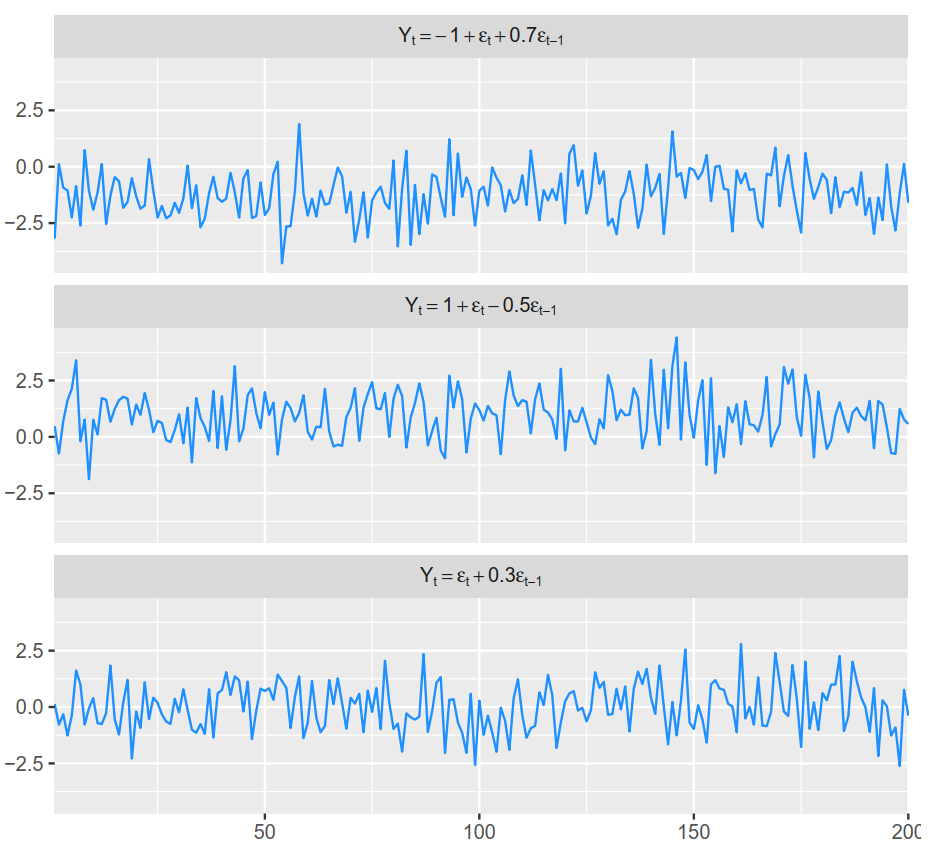
\includegraphics[width=0.6\linewidth]{ma1}
	\label{fig:ma1}
\end{figure}

\subsection{Deriving the Autocorrelation function of the MA(1) process}

While deriving the moments of the MA(1), it became clear that the process is stationary and ergodic to the mean. Note that the time average $\bar{y_t}$ converges to $\mathbb{E}(Y_t)$, the \textit{ensemble average}, the absolute sum of all covariances is clearly finite ($\gamma_j = 0, \forall j > 1$) and the dependence structure depends only on the relative positions of the observations.

Let's use the results of the autocovariances to construct the ACF:

$$\rho_{j} \equiv \frac{\gamma_{j}}{\gamma_{0}}=\left\{\begin{array}{ll}
	1 & j=0 \\
	\frac{\theta}{1+\theta^{2}} & j=\pm 1 \\
	0 & |j|>1
\end{array}\right.$$

Note that the ACF of an MA(1) process is \textit{truncated} in zero for lags greater than 1.

\begin{figure}[h!]
	\centering
	\includegraphics[width=0.6\linewidth]{"fac facp"}
	\label{fig:fac-facp}
\end{figure}

\section{Generalizing the MA model}

We can now generalize the MA(1) model for a moving average of order $q$.

\begin{defn}
	A stationary process $\{Y_t, t \in \mathbb{Z} \}$ is called \textbf{MA(q)}, or a \textbf{moving average of order q}, if it follows the following form:
	$$ Y_t = c + \varepsilon_t + \theta_1 \varepsilon_{t-1} + ... + \theta_q \varepsilon_{t-q}, \hspace{1em} \varepsilon \sim wn(0, \sigma^2), $$
	where $c, \theta_1, ..., \theta_q \in \mathbb{R}, q \in \mathbb{Z}^+$.
\end{defn}

\subsection{Moments of an MA(q) process}

The expected value of an MA(q) is:
$$
\mu \equiv \mathbb{E}\left(Y_{t}\right)=\mathbb{E}\left(c+\varepsilon_{t}+\theta_{1} \varepsilon_{t-1}+\cdots+\theta_{q} \varepsilon_{t-q}\right)=c
$$

Again, using the first result, we can rewrite the model as:
$$
\left(Y_{t}-\mu\right)=\varepsilon_{t}+\theta_{1} \varepsilon_{t-1}+\cdots+\theta_{q} \varepsilon_{t-q}
$$

Multiplying both sides by $\left(Y_{t-j}-\mu\right),$ we have
$$
\begin{aligned}
	\left(Y_{t}-\mu\right)\left(Y_{t-j}-\mu\right) &=\left(\sum_{k=0}^{q} \theta_{k} \varepsilon_{t-k}\right)\left(\sum_{k=0}^{q} \theta_{k} \varepsilon_{t-j-k}\right) \\
	&=\sum_{k=0}^{q} \sum_{\ell=0}^{q} \theta_{k} \theta_{\ell} \varepsilon_{t-k} \varepsilon_{t-j-\ell},
\end{aligned}
$$

where $\theta_{0}=1 .$ Applying the expectation operator, we have:
$$
\gamma_{j}=\left\{\begin{array}{ll}
	\left(\theta_{j}+\theta_{j+1} \theta_{1}+\theta_{j+2} \theta_{2}+\cdots+\theta_{q} \theta_{q-j}\right) \sigma^{2} & |j|=0,1, \ldots, q \\
	0 & |j|>q
\end{array}\right.
$$

\subsection{Deriving the Autocorrelation function of the MA(q) process}

Again, we can clearly see that the MA(q) model is \textit{stationary} and \textit{ergodic.} Note that the time average $\bar{y_t}$ converges to $\mathbb{E}(Y_t)$, the \textit{ensemble average}, the absolute sum of all covariances is clearly finite ($\gamma_j = 0, \forall j > q$) and the dependence structure depends only on the relative positions of the observations.

The autocorrelation function is given by:
$$\rho_{j} \equiv \frac{\gamma_{j}}{\gamma_{0}}=\left\{\begin{array}{ll}
	1 & j=0 \\
	\frac{\theta_{j}+\theta_{j+1} \theta_{1}+\theta_{j+2} \theta_{2}+\cdots+\theta_{q} \theta_{q-j}}{1+\theta_{1}^{2}+\cdots+\theta_{q}^{2}} & |j|=1,2, \ldots, q \\
	0 & |j|>q
\end{array}\right.$$

Now, the ACF is truncated in zero for lags \textit{greater than $q$.}


\section{The MA($\infty$) model}

Consider a special case of a MA(q) model where $q \to \infty$. This yields a moving average of infinite order, MA($\infty$).

\begin{defn}
	A stationary process $\{Y_t, t \in \mathbb{Z} \}$ is called \textbf{MA($\infty$)}, or a \textbf{moving average of infinite order}, if it follows the following form:
	$$ Y_t = c + \sum_{i=0}^{\infty} \theta_i \varepsilon_{t-i}, \hspace{1em} \sim wn(0, \sigma^2), $$
	where $c, \theta_1, ..., \theta_q \in \mathbb{R}, \theta_0 = 1$.
\end{defn}

We also assume that $\sum_{i=0}^{\infty} | \theta_i | < \infty $. This guarantees that the process is \textit{ergodic.}\footnote{Details in Hamilton (1994), Appendix, 3.A.} With this assumption, we can obtain the moments of the MA($\infty$) simply by taking the limit of the finite case MA(q) -- because it enables us to exchange the order between the sum and the expectation operator.

This means that $\mu = c$, as in the previous cases, and:
$$\gamma_{j}=\left(\sum_{i=0}^{\infty} \theta_{j+i} \theta_{i}\right) \sigma^{2}$$

\section{The Wold Decomposition}

This result motivates all ARMA models. It can be defined informally as ``any stationary process has a MA($\infty$) representation''.

\begin{thm}{\textbf{Wold Representation Theorem.}}
	Any process $\{Y_t, t \in \mathbb{Z} \}$ purely nondeterministic can be written as
	$$ Y_t = \mu + \sum_{j=0}^{\infty} \psi_j \varepsilon_{t-j}, $$
	where $\varepsilon_{t} = Y_t - \pi(Y_t | 1, Y_{t-1}, Y_{t-2}, ...)$, i.e., $\varepsilon_{t}$ is the \textit{error of the linear projection of $Y_t$ in $(1, Y_{t-1}, Y_{t-2}, ...)$}.
\end{thm}

\section{Autoregressive models}

Again, we'll begin with its simplest form, AR(1).

\begin{defn} \label{ar1-def}
	A stationary process $\{Y_t, t \in \mathbb{Z} \}$ is called \textbf{AR(1)}, or an \textbf{autoregressive process of order 1}, if it follows the following form:
	$$ Y_t = c + \phi Y_{t-1} + \varepsilon_t, \hspace{1em} \varepsilon_t \sim wn(0, \sigma^2), $$
	where $c, \phi$ are constant.
\end{defn}

\subsection{Moments of an AR(1) process}

With AR($\cdot$) models, we will work in the opposite direction when it comes to stationarity. We'll first \textit{assume} that is holds, and then provide reasoning for why the assumption is valid.

With the assumption of stationarity, we can take expectations and variances on both sides:
$$ \mu = c + \phi \mu \iff \mu = \mathbb{E}(Y_t) = \dfrac{c}{1 - \phi} $$
$$ \gamma_{0} = \phi^2 \gamma_{0} + \sigma^2 \iff \gamma_{0} = Var(Y_t) = \dfrac{\sigma^2}{1 - \phi^2} $$

Using the first result, we can rewrite the model as:
$$ (Y_t - \mu) = \phi (Y_{t-1} - \mu) + \varepsilon_{t} $$

Multiplying both sides by $(Y_{t-j} - \mu)$ and taking expectations yields:
$$ \gamma_{j} = \phi \gamma_{t-j}, \hspace{1em} j = 1,2,... $$

\subsection{Some examples of AR(1) series}

\begin{figure}[h!]
	\centering
	\includegraphics[width=0.6\linewidth]{"ar1"}
	\label{fig:fac-facp}
\end{figure}

\subsection{Autocorrelation function of an AR(1) process}

Given that $\gamma_{j} = \phi \gamma_{t-j}$, it is easy to see that the autocovariance is given by:
$$ \gamma_j = \phi^{|j|} \gamma_0, \hspace{1em} j \in \mathbb{Z} $$

Therefore, $\rho_{j} = \dfrac{\gamma_{j}}{\gamma_{0}} = \phi^{|j|}$.

\subsection{Partial Autocorrelation Function}

Note that $Y_t, Y_{t-2}$ \textit{are correlated.} Can we isolate the correlation between $Y_t, Y_{t-2}$ from the effects of $Y_{t-1}$? 
$$ Cor(Y_t, Y_{t-2} | Y_{t-1}) = Cor(c + \phi Y_{t-1} + \varepsilon_{t}, Y_{t-2} | Y_{t-1}) = 0 $$

This is the intuition behind the \textit{partial autocorrelation function} (PACF). 

\begin{defn}
	The \textbf{partial autocorrelation function} of a stationary process $\{Y_t, t \in \mathbb{Z} \}$ is given by:
$$\alpha_{j}=\left\{\begin{array}{ll}
	\operatorname{Cor}\left(Y_{t}, Y_{t-1}\right)=: \rho_{1} & j=1 \\
	\operatorname{Cor}\left(Y_{t}, Y_{t-j} \mid Y_{t-1}, \ldots, Y_{t-j+1}\right) & j \geq 2
\end{array}\right.$$
\end{defn}

To estimate the ACF of a given time series, we need to use its sample equivalent and a version of the Law of Large Numbers, presented in the previous section, because we're only looking for correlations -- i.e., population moments. To estimate the PACF, that is not enough. We're now looking for \textit{partial correlation.} 

It so happens that OLS gives us the \textit{ceteris paribus} effects. Note that a general form for $\beta$ is given by: $ \beta = \frac{Cov(X,Y)}{Var(X)}$. Therefore, we can estimate using OLS the following models for every $j$: 
$$ Y_t = \beta_0 + \beta_1 Y_{t-1} + ... + \alpha_j Y_{t-j} + u_t $$
The last coefficient of \textit{each regression}, $\hat{\alpha}_j$, is a consistent estimator for $\alpha_{j}$. It is important to highlight, here, that a new model shall be estimated \textit{for each $j$}, as it guarantees that the coefficient $\alpha_{j}$ will be conditional on all $t$ \textit{prior} to $j$.

The following plots showcase ACFs and PACFs for AR(1) processes.

\begin{figure}[h!]
	\centering
	\includegraphics[width=0.6\linewidth]{"fac facp ar1"}
	\label{fig:fac-facp-ar1}
\end{figure}

\subsection{Conditions for stationarity}

When is an AR(1) process stationary? Note that:

$$
\begin{aligned}
	Y_{t} &=c+\phi Y_{t-1}+\varepsilon_{t} \\
	&=c+\phi\left(c+\phi Y_{t-2}+\varepsilon_{t-1}\right)+\varepsilon \\
	&=c+\phi\left(c+\phi\left(c+\phi Y_{t-3}+\varepsilon_{t-2}\right)+\varepsilon_{t-1}\right)+\varepsilon_{t} \\
	& \cdots \\
	&=c \sum_{j=0}^{k-1} \phi^{j}+\phi^{k} Y_{t-k}+\sum_{j=0}^{k-1} \phi^{j} \varepsilon_{t-j}
\end{aligned}
$$

Assuming that $|\phi|<1$ and taking the limit $k \rightarrow \infty,$ we have:

$$
Y_{t}=\frac{c}{1-\phi}+\sum_{j=0}^{\infty} \phi^{j} \varepsilon_{t-j}
$$

The first term follows from the sum of an infinite geometric sequence. This means that \textit{an AR(1) process can be written as a MA($\infty$)} with $\sum_{j = 0}^\infty | \theta_j | < \infty$. Note that this is equivalent to saying that the Wold Representation Theorem holds, with $\mu = \frac{c}{1 - \phi}$, $\psi_j = \phi^j$. This guarantees that the AR(1) process is \textit{stationary} and \textit{ergodic.}

\section{Generalizing the AR model}

\begin{defn}
	A stationary process $\{Y_t, t \in \mathbb{Z} \}$ is called \textbf{AR(p)}, or an \textbf{autoregressive process of order p}, if it follows the following form:
	$$ Y_t = c + \phi Y_{t-1} + ... + \phi_p Y_{t-p} + \varepsilon_t, \hspace{1em} \varepsilon_t \sim wn(0, \sigma^2), $$
	where $c, \phi_1, ..., \phi_p$ are constant.
\end{defn}

\subsection{Moments of an AR(p) process}

Assuming stationarity, we can apply again expectations on both sides:
$$
\mu=c+\phi_{1} \mu+\cdots+\phi_{p} \mu \Longleftrightarrow \mu=\frac{c}{1-\phi_{1}-\cdots-\phi_{p}}
$$

Using this result, we can rewrite the model as:
$$
\left(Y_{t}-\mu\right)=\phi_{1}\left(Y_{t-1}-\mu\right)+\cdots+\phi_{p}\left(Y_{t-p}-\mu\right)+\varepsilon_{t}
$$

Multiplying both sides by $\left(Y_{t-j}-\mu\right)$ and taking expectations, we have:
$$
\gamma_{j}=\left\{\begin{array}{ll}
	\phi_{1} \gamma_{j-1}+\cdots+\phi_{p} \gamma_{j-p} & j=1,2, \ldots \\
	\phi_{1} \gamma_{1}+\cdots+\phi_{p} \gamma_{p}+\sigma^{2} & j=0
\end{array}\right.
$$
Note that the last term in $\gamma_{0}$ is implied by $\mathbb{E}\left(\varepsilon_{t}\right)\left(Y_{t}-\mu\right)=\sigma^{2}$.

\subsection{ACF of an AR(p) process}

Dividing the previous result by $\gamma_{0}$ yields:
$$ \rho_j = \phi_1 \rho_{j-1} + ... + \phi_p \rho_{j-p} $$

Evaluating at $j = 1,2,..., p - 1$ and using $p_i = p_{-i}$, we have the following system of difference equations (aka. Yule-Walker Equations):
$$\left\{\begin{array}{l}
	\rho_{1}=\phi_{1}+\phi_{2} \rho_{1}+\cdots+\phi_{p} \rho_{p-1} \\
	\rho_{2}=\phi_{1} \rho_{1}+\phi_{2}+\cdots+\phi_{p} \rho_{p-2} \\
	\vdots \\
	\rho_{p}=\phi_{1} \rho_{p-1}+\phi_{2} \rho_{p-2}+\cdots+\phi_{p}
\end{array}\right.$$

To solve this, we need to find $\rho_1, \rho_2, ..., \rho_j$ as functions of $\phi_1, \phi_{2}, ..., \phi_j$. The first equation above implies that further correlations from lag $j$ will decay exponentially\footnote{Review this.}. This means that the ACF pattern of an AR(p) looks like the one from the simple AR(1) model.

\section{The Lag Operator}

\begin{defn}
	Given a process $\{Y_t, t \in \mathbb{Z} \},$ the \textbf{lag operator} is defined by:
$$\begin{array}{l}
	L Y_{t}:=Y_{t-1} \\
	L^{2} Y(t):=L\left(L Y_{t}\right)=L\left(Y_{t-1}\right)=Y_{t-2} \\
	\vdots \\
	L^{j} Y(t):=L\left(L\left(L \ldots L Y_{t}\right)=Y_{t-j}\right.
\end{array}$$
\end{defn}

The lag operator is also commutative with multiplication and distributive with regards to addition:
$$ L(cY_t) = c(LY_t) $$
$$ L(Y_t + X_t) = LY_t + LX_t $$

\subsection{The lag operator as a polynomial}

Note that we can use the lag operator as a \textit{polynomial.} We can now rewrite an AR(p) with zero mean as:
$$ (1 - \phi_1 L - \phi_2 L^2 - ... - \phi_p L^p)Y_t = \varepsilon_{t} $$

Note that the term multiplying $Y_t$ \textit{is a polynomial in L.} We denote this by:
$$ \Phi_p (L) Y_t = \varepsilon_{t} $$

Analogously, we can rewrite an MA(q) process as:
$$\begin{aligned}
	Y_{t} &=\varepsilon_{t}+\theta_{1} \varepsilon_{t-1}+\theta_{2} \varepsilon_{t-2}+\cdots+\theta_{q} \varepsilon_{t-q} \\
	&=\left(1+\theta_{1} L+\theta_{2} L^{2}+\cdots+\theta_{q} L^{q}\right) \varepsilon_{t} \\
	& \equiv \Theta_{q}(L) \varepsilon_{t}
\end{aligned}$$

We would also like to define an operator $(1 - \phi L)^{-1}$ such that:
$$ (1 - \phi L)^{-1} (1 - \phi L) = 1 $$

$(1 - \phi L)^{-1}$ is well defined when $|\phi| < 1$ and the following condition holds\footnote{Hamilton (1994), p. 27-29.}:
$$ (1 - \phi L)^{-1} := 1 + \phi L + \phi^2 L^2 + \phi^3 L^3 + ... $$

From this, we can rewrite the AR(1) as a MA($\infty$) by multiplying the AR by $(1 - \phi L)^{-1}$ on both sides:
$$ Y_t = (1 - \phi L)^{-1} \varepsilon_{t}$$

The $(1 - \phi L)^{-1}$ operator will be very useful to translate models between AR and MA representations, aside from highlighting the conditions of stationarity for the process.


\subsection{Stationarity and the lag operator}

We can factor out the polynomial of an AR(p) process as:
$$ 1 - \phi_1 L - ... - \phi_{p} L^p = (1 - \lambda_1 L)...(1 - \lambda_p L), $$
where $\lambda_j = \frac{1}{a_j} \forall j = 1,..., p$ and $a_1, ..., a_p$ are the $p$ roots of a polynomial of $p$-th degree. This means that we can rewrite the AR(p) process as:
$$ (1 - \lambda_1 L)...(1 - \lambda_p L) Y_t = \varepsilon_{t} $$

If $|\lambda_p | < 1$ (or, equivalently, $|a_j > 1$) $\forall j = 1, ..., p$, then \textit{the inverse polynomial exists} and we can write the AR(p) process as a MA($\infty$) -- which \textit{we know to be stationary}:
$$\begin{aligned}
	Y_{t} &=\left(1-\lambda_{1} L\right)^{-1} \ldots\left(1-\lambda_{p} L\right)^{-1} \varepsilon_{t} \\
	&=:\left(1+\psi_{1} L+\psi_{2} L^{2}+\ldots\right) \varepsilon_{t} \\
	&=: \Psi_{\infty}(L) \varepsilon_{t}
\end{aligned}$$

\section{Finally, the ARMA(p,q) process}

An ARMA(p,q) model is created by combining an AR(p) with a MA(q).

\begin{defn}
	A stationary process $\{Y_t, t \in \mathbb{Z} \}$ is called \textbf{ARMA(p,q)}, or an \textbf{autoregressive-moving average process of order (p,q)}, if it follows the following form:
	$$ Y_t = c + \phi Y_{t-1} + ... + \phi_p Y_{t-p} + \theta_1 \varepsilon_{t-1} + ... + \theta_q \varepsilon_{t-q} + \varepsilon_t, \hspace{1em} \varepsilon_t \sim wn(0, \sigma^2), $$
	where $c, \theta_1, ..., \theta_p, \phi_1, ..., \phi_q$ are constant, $p, q \in \mathbb{Z}^+$.
\end{defn}

Using the lag operator yields an alternate form for the ARMA(p,q) process:
$$\begin{aligned}
	\left(1-\phi_{1} L-\cdots-\phi_{p} L^{p}\right) Y_{t} &=c+\left(1+\theta_{1} L+\cdots+\theta_{q} L^{q}\right) \varepsilon_{t} \\
	\Phi_{p}(L) Y_{t} &=c+\Theta_{q}(L) \varepsilon_{t}
\end{aligned}$$

\subsection{Stationarity and invertibility of an ARMA(p,q) process}

\textbf{Stationarity} depends only on the AR part of the process, because all MA($\cdot$) are stationary. It is sufficient to verifiy that \textit{the roots of the polynomial $\Phi_p(L)$ are out of the unit circle:}
$$\Phi_p(L) = 1 - \phi_1 L - \phi_2 L^2 - ... - \phi_{p} L^p $$

\textbf{Invertibility} depends only on the MA part of the process, because it needs to be able to be rewritten as a linear combination of its past values plus the contemporaneous error term $\varepsilon_{t}$:
$$ Y_t = \alpha + \sum_{s=1}^{\infty} \pi Y_{t-s} + \varepsilon_{t} $$
for some $\alpha$ and \{$\pi_j$\}. 

\begin{quote}
Consider, for example, the case of $M A(1)$ with $\mu=0$
$$
y_{t}=\varepsilon_{t}+\theta \varepsilon_{t-1}
$$
which can be rewritten as
$$
\varepsilon_{t}=y_{t}-\theta \varepsilon_{t-1}
$$
Repeated substitution of this relation for the lagged $\varepsilon_{t-s}$ terms yields
$$
\begin{aligned}
	\varepsilon_{t} &=y_{t}-\theta\left(y_{t-1}-\theta \varepsilon_{t-2}\right) \\
	&=y_{t}-\theta y_{t-1}+\theta^{2} \varepsilon_{t-2} \\
	& \cdots \\
	&=y_{t}-\theta y_{t-1}+\ldots+(-\theta)^{p} y_{t-p}+(-\theta)^{p+1} \varepsilon_{t-p+1}
\end{aligned}
$$
If $|\theta|<1,$ then the last term in this expression tends to zero in mean-square as $p \rightarrow \infty,$ so that it make
sense to write
$$
\varepsilon_{t}=y_{t}+\sum_{s=1}^{\infty}(-\theta)^{s} y_{t-s}
$$
Or
$$
y_{t}=\varepsilon_{t}+\sum_{s=1}^{\infty}(-\theta)^{s} y_{t-s}
$$
so $|\theta|<1$ is the sufficient condition for a $M A(1)$ process to be invertible. (Powell, Conditions for Stationarity and Invertibility, UC Berkeley.)
\end{quote}

In other words, because AR($\cdot$) models \textit{with roots of the polynomial outside of the unit circle} are invertible, being able to write the MA(q) part of the process as an AR($\infty$) with the root condition is sufficient to guarantee invertibility.

\subsection{Moments of an ARMA(p,q) process}

If the process is stationary, $\Phi_{p}^{-1}(L)$ exists and we can rewrite ARMA $(\mathrm{p}, \mathrm{q})$ as $\mathrm{MA}(\infty)$
$$
Y_{t}=\mu+\Psi_{\infty}(L) \varepsilon_{t}
$$
where
$$
\mu \equiv \frac{c}{\Phi(1)} ; \quad \Phi(1)=1-\sum_{j=1}^{p} \phi_{j} ; \quad \Psi_{\infty}(L) \equiv \Phi_{p}(L)^{-1} \Theta_{q}(L)
$$
From the results derived for MA(q) we have for $q=\infty$
$$
\begin{aligned}
	\mathbb{E}\left(Y_{t}\right) &=\mu \\
	\gamma_{j} &=\left(\sum_{i=0}^{\infty} \psi_{j+i} \psi_{j}\right) \sigma^{2}
\end{aligned}
$$
where $\psi_{0}=1$

\subsection{ACF of an ARMA(p,q) process}

It is usually easy to identify an AR(p) or MA(q) visually by inspecting its ACF and PACF, because AR's PACF is truncated on $p$, MA's ACF is truncated on $q$. For ARMA(p,q) models it is more complicated: both functions are not truncated! Note, however, that in that case, the ACF decays geometrically after lag $q$ and the PACF decays geometrically after lag $p$.

\vspace{1em}

\begin{center}


\begin{tabular}{|c|c|c|}
	\hline
	\textbf{Model}  &\textbf{ ACF }& \textbf{PACF} \\
	\hline
	\textbf{AR($p$)} & Decays & Truncated after lag $p$ \\
	\hline
	\textbf{MA($q$)} & Truncated after lag $q$ & Decays \\
	\hline
	\textbf{ARMA($p,q$)} & Decays after lag $q$ & Decays after lag $p$ \\
	\hline
\end{tabular}


\end{center}

\section{Testing for time dependence} %% Material complementar


We've seen that a sufficient condition for ergodicity is convergence of the absolute sum of all covariances. This presents a problem: how can we \textit{estimate} these covariances?

Let $Z_t$ be our series to be tested. Denote the autocovariance of order $j$ as $\gamma_{j} := Cov(Z_t, Z_{t-j})$. We can try to estimate these parameters with its sample equivalents: 
$$ \bar{z_t} := \dfrac{1}{T} \sum_{t=1}^{T} z_t $$
$$ \hat{\gamma}_{j} := \dfrac{1}{T - j - 1} \sum_{t = j+1}^{T} (z_t - \bar{z_t})(z_{t-j} - \bar{z_t}) $$

But this is not as simple as it seems. We know that $\hat{\gamma}_{j}$ converges almost sure to $\gamma_{j}$ \textit{if the process is ergodic.} If it \textit{isn't,} the information from $\hat{\gamma}_{j}$ may not be reliable -- after all, we won't have a Law of Large Numbers! 

Our solution to this problem won't be very rigorous here. We'll plot $\{\hat{\gamma}_{j}, j \in \mathbb{N}\}$ and check if it looks stationary. If the series passes this intuitive test, we can assume that $\{\hat{\gamma}_{j}, j \in \mathbb{N}\}$ will be informative about $\{{\gamma}_{j}, j \in \mathbb{N}\}$. 

The visual inspection should focus on two main factors: (i) constant mean over time; (ii) constant variance over time. Here are some examples of series to be inspected:

\begin{figure}[h!]
	\centering
	\includegraphics[width=0.6\linewidth]{"exemplos ts"}
	\label{fig:exemplos-ts}
\end{figure}

After plotting the time series and assuring that it is well behaved, we can plot its \textit{correlogram:} $\{ \hat{\rho}_{j} := \frac{\hat{\gamma}_{j}}{\hat{\gamma}_{0}}, j \in \mathbb{N}\}$. If its sum looks convergent, we will assume that the process is \textit{stationary} and \textit{ergodic} -- which will enable us to use sample equivalents as representations of population parameters.

\subsection{Hypothesis testing}

Consider this correlogram:

\begin{figure}
	\centering
	\includegraphics[width=0.6\linewidth]{"correlograma rx"}
	\label{fig:correlograma-rx}
\end{figure}

This series appears to not be correlated with its past. How can we test this? 
$$ H_0 = \rho_j = 0, \forall j \neq 0 $$
This implies, in theory, that we would need to test infinite correlations. In practice, we limit the range to an arbitrary $J$. Let $\hat{\rho} := (\hat{\rho}_1, \hat{\rho}_2, ..., \hat{\rho}_J)^T, \rho = (\rho_1, \rho_2, ..., \rho_J)^T.$ Under the null, $\rho = 0$, and as $T \to \infty$:
$$ \sqrt{T}\hat{\rho} \to \mathcal{N}(0, I_J) $$
The intuition here is that, under $H_0$, $\hat{\rho}$ is a sequence of \textit{iid} variables with mean zero and variance-covariance matrix $I_J$ -- which makes the CLT valid. 

Given this result, we can now create a statistic that does not depend on the multivariate normal distribution. We will square and sum the expression to arrive at a Chi-squared distribution. This enables us to test the hypothesis with a Wald statistic. Under the null:

$$
W_{T}=T \hat{\rho}^{T} \hat{\rho}=T \sum_{j=1}^{J} \hat{\rho_{j}}^{2} \rightarrow \chi_{J}^{2}
$$

\subsection{Testing autocorrelations or regressions?}

Note that inferring about the autocorrelations is intimately related to inferring in a regression of a time series on its past values. This can be understood by remembering the linear projection interpretation of OLS. Ordinary Least Squares estimation \textit{always} reports the parameters of the linear projection of $Y$ in $X$, no matter how the model is specified!

Consider the following model:
$$
\begin{aligned}
	Y_{t} &=\alpha+\beta_{1} Y_{t-1}+\beta_{2} Y_{t-2}+\cdots+\beta_{J} Y_{t_{J}}+\varepsilon_{t} \\
	&=\alpha+X_{t} \beta+\varepsilon_{t}
\end{aligned}
$$
where $\beta:=\left(\beta_{1}, \ldots, \beta_{J}\right)^{T}$ and $X_{t}=\left(Y_{t-1}, \ldots, Y_{t-j}\right) .$ If we define the coefficients of the model above as the parameters of the linear projection of $Y_t$ on the unit vector and $X_t$, $\alpha=\mu_{Y}-\mu_{X} \beta$ where $\mu_{Y}=\mathrm{E}\left(Y_{t}\right)$ and $\mu_{X}=\mathrm{E}\left(X_{t}\right)$

Using this result, we have:
$$
Y_{t}-\mu_{Y}=\left(X_{t}-\mu_{X}\right) \beta+\varepsilon_{t}
$$
This means that $\beta$ can be written as:
$$
\beta=\mathbb{E}\left[\left(X_{t}-\mu_{X}\right)^{T}\left(X_{t}-\mu_{X}\right)\right]^{-1} \mathbb{E}\left[\left(X_{t}-\mu_{X}\right)^{T}\left(Y_{t}-\mu_{Y}\right)\right]=\Gamma^{-1} \gamma
$$
where the matrix $\Gamma^{-1}$ is symmetric with diagonal elements all equal to $\gamma_{1}, \gamma_{2}, \ldots, \gamma_{J-1}$, due to the assumed stationarity. Note that $\mathbb{E}(Y_t - \mu_Y)^2 = \mathbb{E}(Y_{t-j} - \mu_{Y-j})^2 = \gamma_0 \forall j$.

Thus, $\beta=\overrightarrow{0} \Longleftrightarrow \gamma=\overrightarrow{0}$, because $\Gamma$ is a positive definite matrix. This means that \textit{testing $\beta = 0$ is equivalent to testing $\gamma = 0$.}

It is important to highlight that this analysis is based upon the inference of $\gamma_{j}=\mathbb{E}\left(z_{t}-\bar{z}_{T}\right)\left(z_{t-j}-\bar{z}_{T}\right).$ If we were interested in \textit{other types of relations between $Z_t$ and its past, the analysis would have to be adapted} -- for example, $Z_t^2$. It would be necessary to check again for stationarity and ergodicity.


\chapter{Problem 1: Modelling exchange rates}

Loading the database and creating dummy variables:

\begin{Shaded}
\begin{Highlighting}[]
\NormalTok{df <-}\StringTok{ }\KeywordTok{read_excel}\NormalTok{(}\StringTok{"RS_USD.xlsx"}\NormalTok{)}


\KeywordTok{names}\NormalTok{(df)[}\KeywordTok{names}\NormalTok{(df) }\OperatorTok{==}\StringTok{ "R$/US$"}\NormalTok{] <-}\StringTok{ "p"}

\KeywordTok{names}\NormalTok{(df)[}\KeywordTok{names}\NormalTok{(df) }\OperatorTok{==}\StringTok{ "Variação (em %)"}\NormalTok{] <-}\StringTok{ "delta"}

\KeywordTok{names}\NormalTok{(df)[}\KeywordTok{names}\NormalTok{(df) }\OperatorTok{==}\StringTok{ "Data"}\NormalTok{] <-}\StringTok{ "date"}

\NormalTok{sign <-}\StringTok{ }\KeywordTok{as.numeric}\NormalTok{(df}\OperatorTok{$}\NormalTok{delta }\OperatorTok{>}\StringTok{ }\DecValTok{0}\NormalTok{)}

\NormalTok{count <-}\StringTok{ }\KeywordTok{c}\NormalTok{(}\DecValTok{1}\OperatorTok{:}\DecValTok{2153}\NormalTok{)}

\NormalTok{df <-}\StringTok{ }\KeywordTok{data.frame}\NormalTok{(count, df, sign)}
\end{Highlighting}
\end{Shaded}

Before constructing our models, we need to check (intuitively) if the
series at hand is \emph{stationary} and \emph{ergodic}. For this, we're
going to plot the time series, its autocorrelations and partial
autocorrelations.

\begin{Shaded}
\begin{Highlighting}[]
\NormalTok{pplot <-}\StringTok{ }\KeywordTok{ggplot}\NormalTok{(}\DataTypeTok{data =}\NormalTok{ df, }\KeywordTok{aes}\NormalTok{(}\DataTypeTok{x =}\NormalTok{ date, }\DataTypeTok{y =}\NormalTok{ p)) }\OperatorTok{+}\StringTok{ }\KeywordTok{geom_line}\NormalTok{() }\OperatorTok{+}\StringTok{ }
\StringTok{    }\KeywordTok{ggtitle}\NormalTok{(}\StringTok{"USD/BRL, Price"}\NormalTok{) }\OperatorTok{+}\StringTok{ }\KeywordTok{theme_few}\NormalTok{()}
\NormalTok{pplot}
\end{Highlighting}
\end{Shaded}

\begin{center}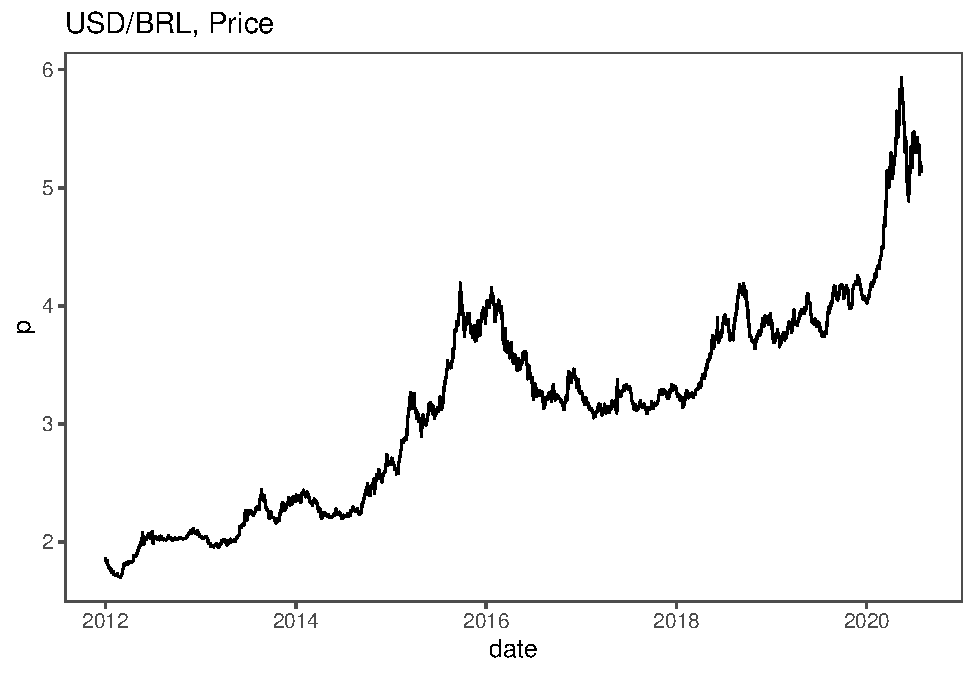
\includegraphics{Econo2_P1_files/figure-latex/plots-1} \end{center}

\begin{Shaded}
\begin{Highlighting}[]
\NormalTok{deltaplot <-}\StringTok{ }\KeywordTok{ggplot}\NormalTok{(}\DataTypeTok{data =}\NormalTok{ df, }\KeywordTok{aes}\NormalTok{(}\DataTypeTok{x =}\NormalTok{ date, }\DataTypeTok{y =}\NormalTok{ delta)) }\OperatorTok{+}\StringTok{ }\KeywordTok{geom_line}\NormalTok{() }\OperatorTok{+}\StringTok{ }
\StringTok{    }\KeywordTok{ggtitle}\NormalTok{(}\StringTok{"USD/BRL, %"}\NormalTok{) }\OperatorTok{+}\StringTok{ }\KeywordTok{theme_few}\NormalTok{()}
\NormalTok{deltaplot}
\end{Highlighting}
\end{Shaded}

\begin{center}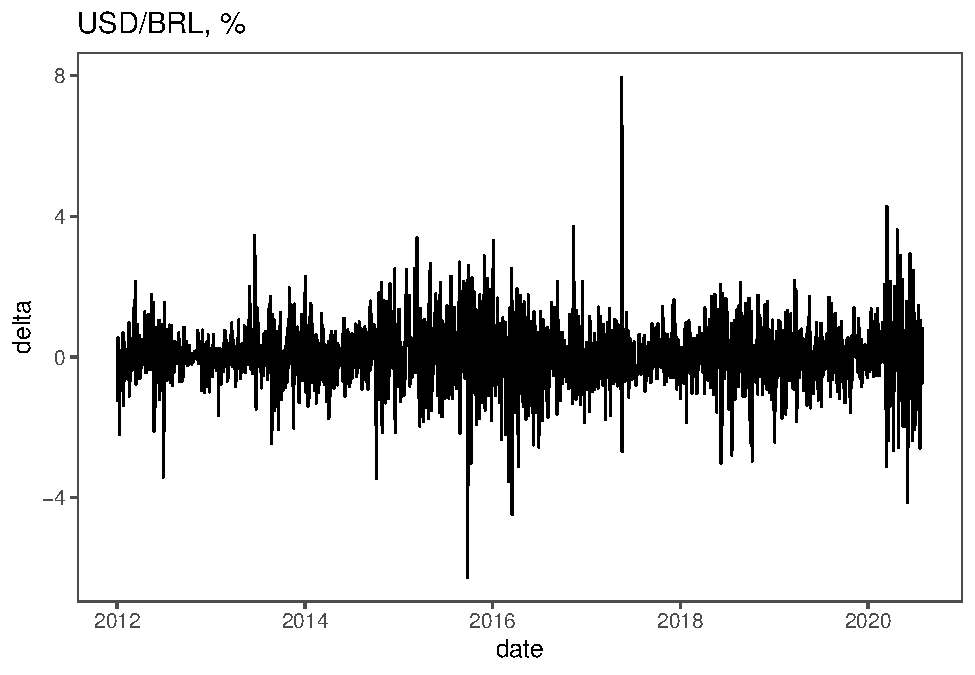
\includegraphics{Econo2_P1_files/figure-latex/plots-2} \end{center}

\begin{Shaded}
\begin{Highlighting}[]
\NormalTok{dummyplot <-}\StringTok{ }\KeywordTok{ggplot}\NormalTok{(}\DataTypeTok{data =}\NormalTok{ df, }\KeywordTok{aes}\NormalTok{(}\DataTypeTok{x =}\NormalTok{ count, }\DataTypeTok{y =}\NormalTok{ sign)) }\OperatorTok{+}\StringTok{ }\KeywordTok{geom_line}\NormalTok{() }\OperatorTok{+}\StringTok{ }
\StringTok{    }\KeywordTok{ggtitle}\NormalTok{(}\StringTok{"USD/BRL, +/-"}\NormalTok{) }\OperatorTok{+}\StringTok{ }\KeywordTok{xlim}\NormalTok{(}\DecValTok{1}\NormalTok{, }\DecValTok{200}\NormalTok{) }\OperatorTok{+}\StringTok{ }\KeywordTok{theme_few}\NormalTok{()}
\NormalTok{dummyplot}
\end{Highlighting}
\end{Shaded}

\begin{verbatim}
## Warning: Removed 1953 row(s) containing missing values (geom_path).
\end{verbatim}

\begin{center}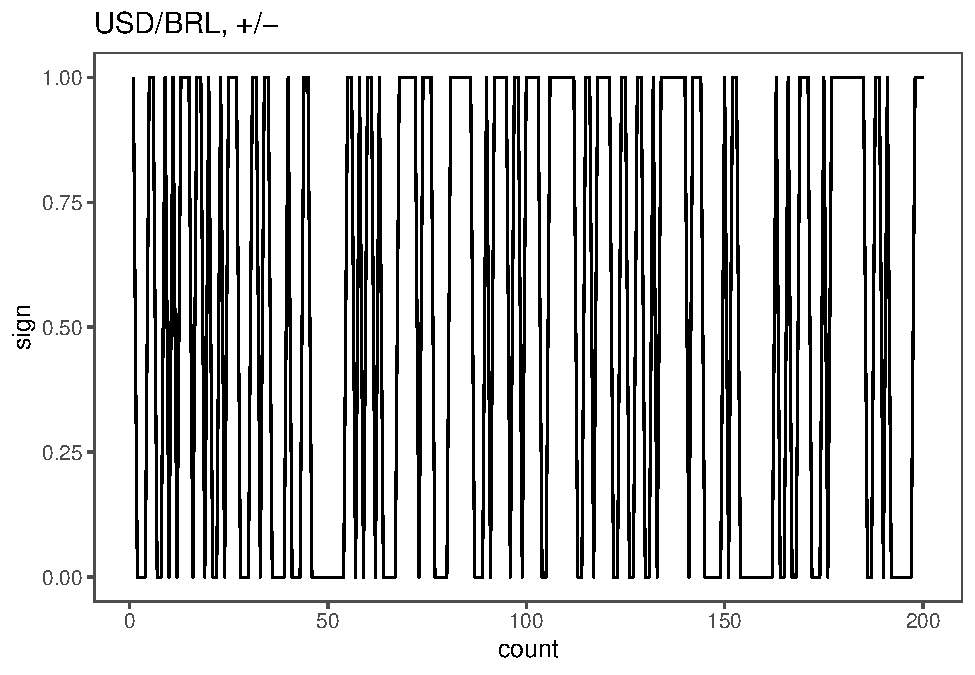
\includegraphics{Econo2_P1_files/figure-latex/plots-3} \end{center}

\begin{Shaded}
\begin{Highlighting}[]
\CommentTok{# For delta}

\NormalTok{acf_delta <-}\StringTok{ }\KeywordTok{Acf}\NormalTok{(df}\OperatorTok{$}\NormalTok{delta, }\DataTypeTok{lag.max =} \DecValTok{5000}\NormalTok{)}
\end{Highlighting}
\end{Shaded}

\begin{center}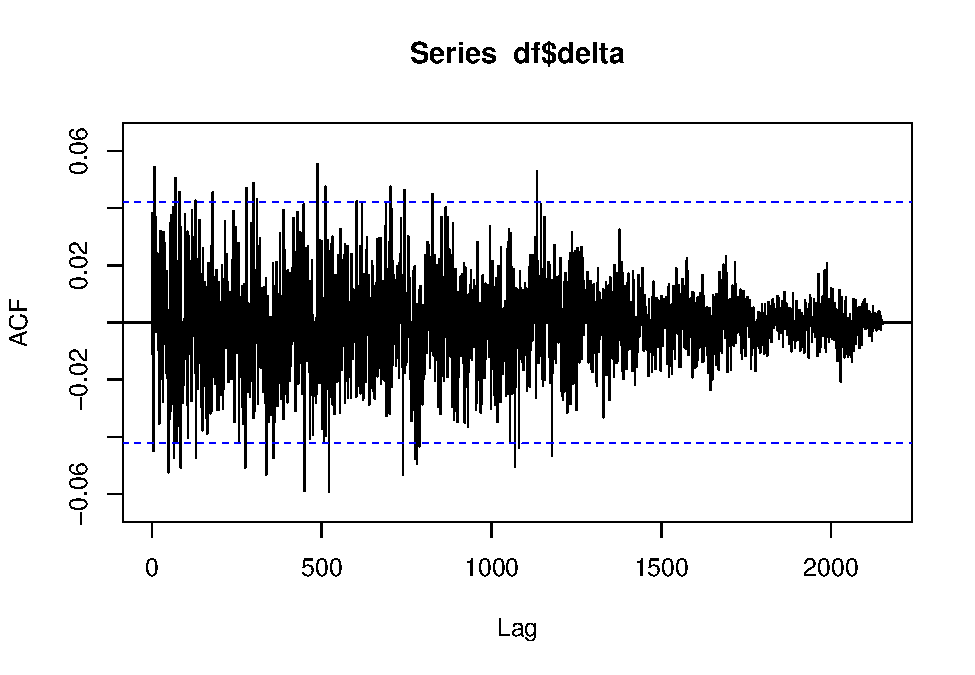
\includegraphics{Econo2_P1_files/figure-latex/plots-4} \end{center}

\begin{Shaded}
\begin{Highlighting}[]
\NormalTok{acf_test_values <-}\StringTok{ }\NormalTok{acf_delta}\OperatorTok{$}\NormalTok{acf}\OperatorTok{/}\KeywordTok{sd}\NormalTok{(acf_delta}\OperatorTok{$}\NormalTok{acf)}

\KeywordTok{head}\NormalTok{(}\KeywordTok{data.frame}\NormalTok{(acf_test_values))}
\end{Highlighting}
\end{Shaded}

\begin{verbatim}
##   acf_test_values
## 1      37.9547672
## 2       1.4506537
## 3      -0.4173129
## 4       0.2125873
## 5      -1.7053782
## 6       0.5358210
\end{verbatim}

\begin{Shaded}
\begin{Highlighting}[]
\NormalTok{facst <-}\StringTok{ }\KeywordTok{ggAcf}\NormalTok{(df}\OperatorTok{$}\NormalTok{delta, }\DataTypeTok{type =} \StringTok{"correlation"}\NormalTok{, }\DataTypeTok{lag.max =} \DecValTok{20}\NormalTok{, }
    \DataTypeTok{plot =}\NormalTok{ T) }\OperatorTok{+}\StringTok{ }\KeywordTok{theme_few}\NormalTok{()}
\NormalTok{faclt <-}\StringTok{ }\KeywordTok{ggAcf}\NormalTok{(df}\OperatorTok{$}\NormalTok{delta, }\DataTypeTok{type =} \StringTok{"correlation"}\NormalTok{, }\DataTypeTok{lag.max =} \DecValTok{5000}\NormalTok{, }
    \DataTypeTok{plot =}\NormalTok{ T) }\OperatorTok{+}\StringTok{ }\KeywordTok{theme_few}\NormalTok{()}

\NormalTok{facpst <-}\StringTok{ }\KeywordTok{ggPacf}\NormalTok{(df}\OperatorTok{$}\NormalTok{delta, }\DataTypeTok{type =} \StringTok{"correlation"}\NormalTok{, }\DataTypeTok{lag.max =} \DecValTok{100}\NormalTok{, }
    \DataTypeTok{plot =}\NormalTok{ T) }\OperatorTok{+}\StringTok{ }\KeywordTok{theme_few}\NormalTok{()}
\end{Highlighting}
\end{Shaded}

\begin{verbatim}
## Warning: Ignoring unknown parameters: type
\end{verbatim}

\begin{Shaded}
\begin{Highlighting}[]
\NormalTok{facplt <-}\StringTok{ }\KeywordTok{ggPacf}\NormalTok{(df}\OperatorTok{$}\NormalTok{delta, }\DataTypeTok{type =} \StringTok{"correlation"}\NormalTok{, }\DataTypeTok{lag.max =} \DecValTok{5000}\NormalTok{, }
    \DataTypeTok{plot =}\NormalTok{ T) }\OperatorTok{+}\StringTok{ }\KeywordTok{theme_few}\NormalTok{()}
\end{Highlighting}
\end{Shaded}

\begin{verbatim}
## Warning: Ignoring unknown parameters: type
\end{verbatim}

\begin{Shaded}
\begin{Highlighting}[]
\NormalTok{facst}
\end{Highlighting}
\end{Shaded}

\begin{center}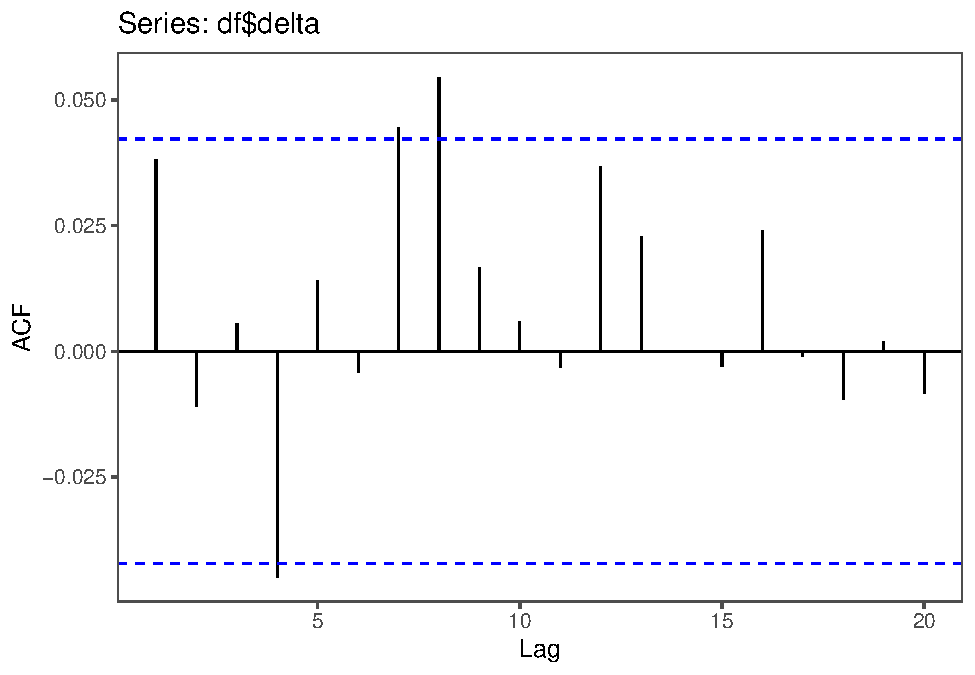
\includegraphics{Econo2_P1_files/figure-latex/plots-5} \end{center}

\begin{Shaded}
\begin{Highlighting}[]
\NormalTok{faclt}
\end{Highlighting}
\end{Shaded}

\begin{center}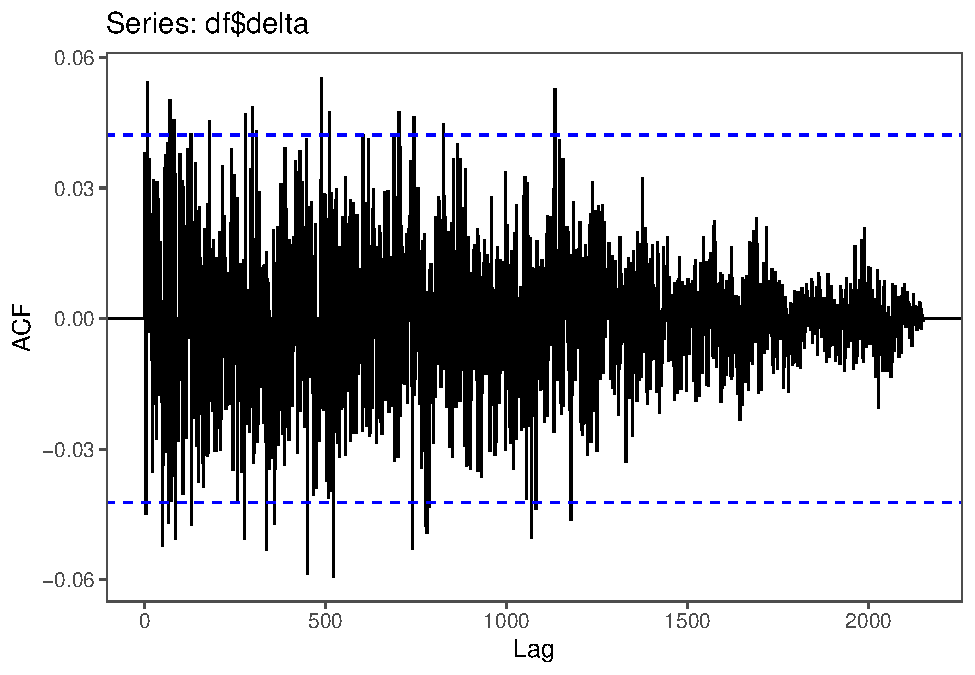
\includegraphics{Econo2_P1_files/figure-latex/plots-6} \end{center}

\begin{Shaded}
\begin{Highlighting}[]
\NormalTok{facpst}
\end{Highlighting}
\end{Shaded}

\begin{center}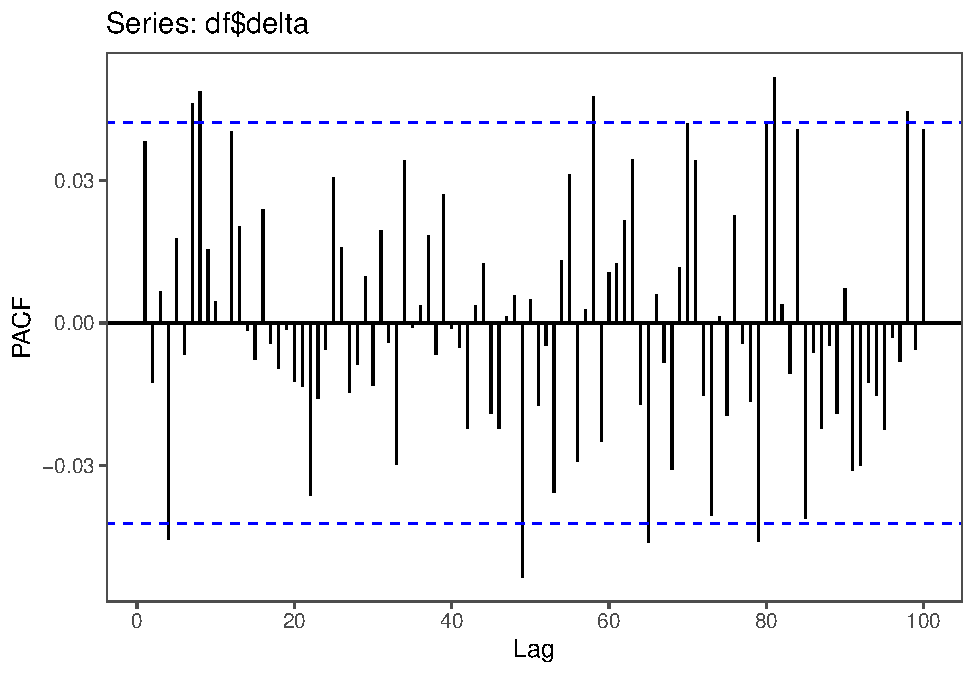
\includegraphics{Econo2_P1_files/figure-latex/plots-7} \end{center}

\begin{Shaded}
\begin{Highlighting}[]
\NormalTok{facplt}
\end{Highlighting}
\end{Shaded}

\begin{center}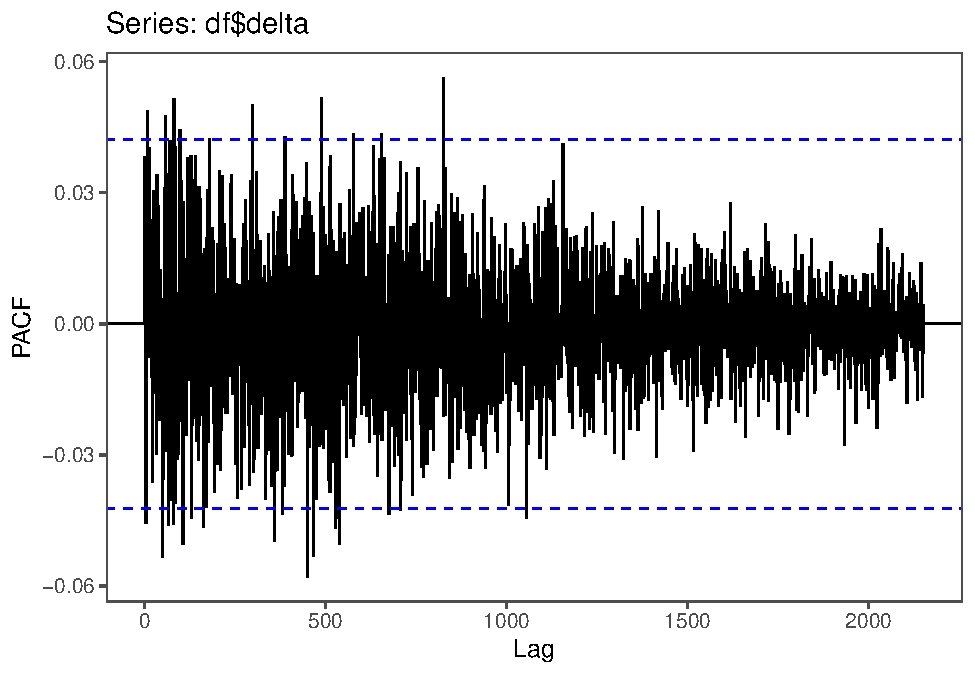
\includegraphics{Econo2_P1_files/figure-latex/plots-8} \end{center}

\begin{Shaded}
\begin{Highlighting}[]
\NormalTok{facst2 <-}\StringTok{ }\KeywordTok{ggAcf}\NormalTok{((df}\OperatorTok{$}\NormalTok{delta)}\OperatorTok{^}\DecValTok{2}\NormalTok{, }\DataTypeTok{type =} \StringTok{"correlation"}\NormalTok{, }\DataTypeTok{lag.max =} \DecValTok{20}\NormalTok{, }
    \DataTypeTok{plot =}\NormalTok{ T) }\OperatorTok{+}\StringTok{ }\KeywordTok{theme_few}\NormalTok{()}
\NormalTok{facst2}
\end{Highlighting}
\end{Shaded}

\begin{center}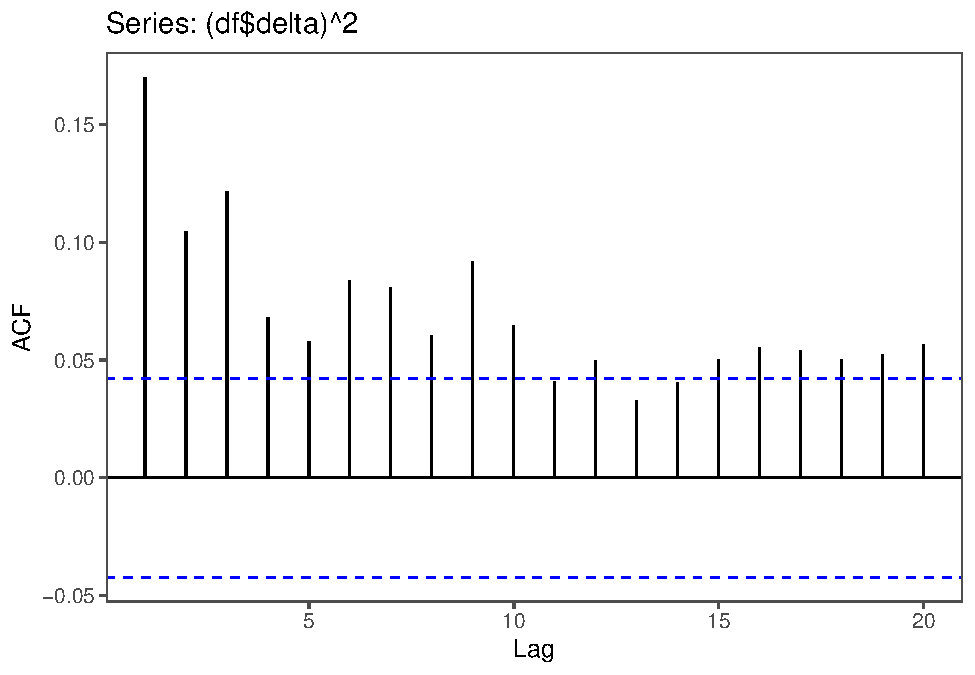
\includegraphics{Econo2_P1_files/figure-latex/plots-9} \end{center}

Let's now create our first ARMA models (equivalent to ARIMA with 2nd
argument = 0). We'll begin with the first hypothesis:
\(\mathbb{P}(+) = \mathbb{P}(-).\) Modelling this with an AR(1), we
have:

\[Sign_{t+1} = \alpha + \beta Sign_t + \varepsilon, \hspace{2em} \varepsilon \sim wn(0, \sigma^2)\]
In R, we'll use the package \emph{forecast} to construct this model:

\begin{Shaded}
\begin{Highlighting}[]
\NormalTok{AR1sign <-}\StringTok{ }\KeywordTok{Arima}\NormalTok{(df}\OperatorTok{$}\NormalTok{sign, }\DataTypeTok{order =} \KeywordTok{c}\NormalTok{(}\DecValTok{1}\NormalTok{, }\DecValTok{0}\NormalTok{, }\DecValTok{0}\NormalTok{))}
\KeywordTok{summary}\NormalTok{(AR1sign)}
\end{Highlighting}
\end{Shaded}

\begin{verbatim}
## Series: df$sign 
## ARIMA(1,0,0) with non-zero mean 
## 
## Coefficients:
##          ar1    mean
##       0.0278  0.5165
## s.e.  0.0215  0.0111
## 
## sigma^2 estimated as 0.2498:  log likelihood=-1560.63
## AIC=3127.26   AICc=3127.27   BIC=3144.28
## 
## Training set error measures:
##                        ME      RMSE       MAE  MPE MAPE     MASE          ACF1
## Training set 2.157119e-05 0.4995356 0.4990724 -Inf  Inf 1.027755 -0.0006313563
\end{verbatim}

\begin{Shaded}
\begin{Highlighting}[]
\KeywordTok{plot}\NormalTok{(AR1sign)}
\end{Highlighting}
\end{Shaded}

\begin{center}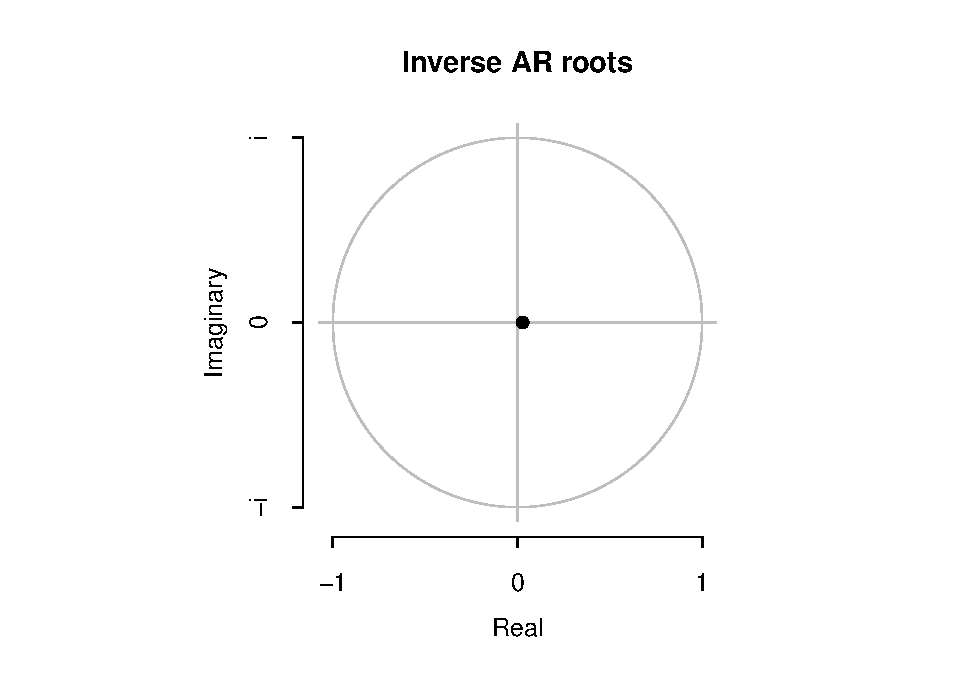
\includegraphics{Econo2_P1_files/figure-latex/AR(1)-1} \end{center}

\begin{Shaded}
\begin{Highlighting}[]
\KeywordTok{tsdisplay}\NormalTok{(AR1sign}\OperatorTok{$}\NormalTok{residuals)}
\end{Highlighting}
\end{Shaded}

\begin{center}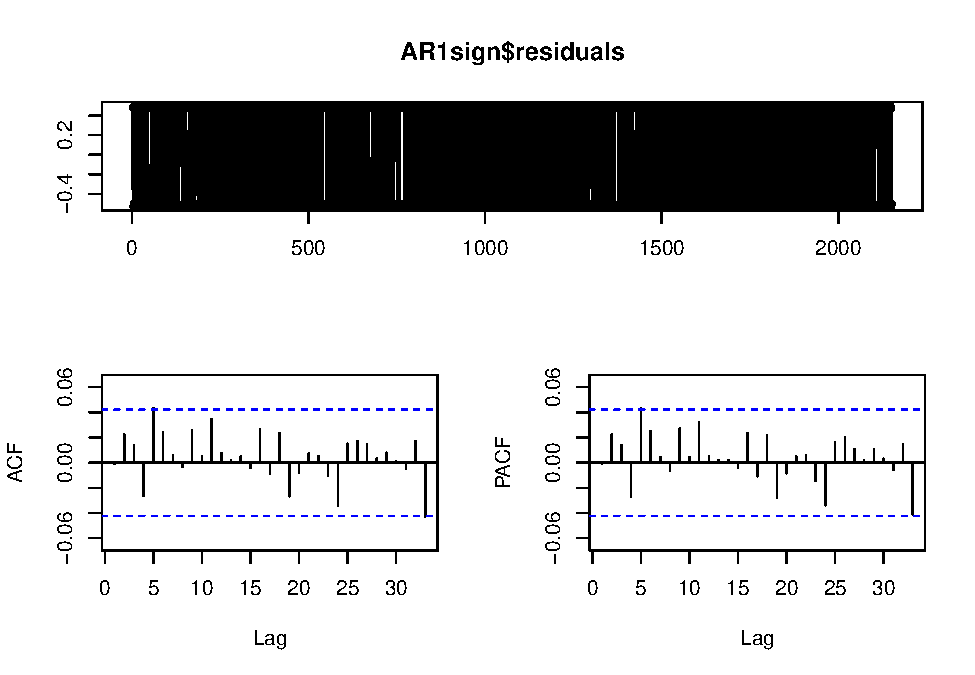
\includegraphics{Econo2_P1_files/figure-latex/AR(1)-2} \end{center}

With the results of the summary, we can now apply a hypothesis test for
our first
question.\footnote{Testing $\beta$ is equivalent to testing $\gamma$.}

\[ H_0: \beta = 0\] \[H_1: \beta \neq 0\]

\(\dfrac{\hat{ar_1} - ar_1}{s.e.(ar_1)}\):

\begin{Shaded}
\begin{Highlighting}[]
\NormalTok{AR1sign}\OperatorTok{$}\NormalTok{coef[}\DecValTok{1}\NormalTok{]}\OperatorTok{/}\KeywordTok{sqrt}\NormalTok{(AR1sign}\OperatorTok{$}\NormalTok{var.coef[}\DecValTok{1}\NormalTok{, }\DecValTok{1}\NormalTok{])}
\end{Highlighting}
\end{Shaded}

\begin{verbatim}
##      ar1 
## 1.287942
\end{verbatim}

The second hypothesis in the problem refers to the delta of the
variation: \[\mathbb{E}(\Delta | + ) \neq \mathbb{E}(\Delta | - ).\]

\[\Delta_{t+1} = \alpha + \beta Sign_t + \varepsilon, \hspace{2em} \varepsilon \sim wn(0, \sigma^2).\]

\begin{Shaded}
\begin{Highlighting}[]
\NormalTok{lmsignt <-}\StringTok{ }\KeywordTok{lm}\NormalTok{(delta }\OperatorTok{~}\StringTok{ }\KeywordTok{lag}\NormalTok{(df}\OperatorTok{$}\NormalTok{sign, }\DataTypeTok{k =} \DecValTok{1}\NormalTok{), }\DataTypeTok{data =}\NormalTok{ df)}
\KeywordTok{summary}\NormalTok{(lmsignt)}
\end{Highlighting}
\end{Shaded}

\begin{verbatim}
## 
## Call:
## lm(formula = delta ~ lag(df$sign, k = 1), data = df)
## 
## Residuals:
##     Min      1Q  Median      3Q     Max 
## -6.3285 -0.4706 -0.0060  0.4655  7.9442 
## 
## Coefficients:
##                     Estimate Std. Error t value Pr(>|t|)
## (Intercept)          0.01293    0.02811   0.460    0.646
## lag(df$sign, k = 1)  0.05802    0.03911   1.484    0.138
## 
## Residual standard error: 0.9066 on 2150 degrees of freedom
##   (1 observation deleted due to missingness)
## Multiple R-squared:  0.001023,   Adjusted R-squared:  0.000558 
## F-statistic: 2.201 on 1 and 2150 DF,  p-value: 0.1381
\end{verbatim}

\begin{Shaded}
\begin{Highlighting}[]
\KeywordTok{ggplot}\NormalTok{(df, }\KeywordTok{aes}\NormalTok{(}\DataTypeTok{x =} \KeywordTok{lag}\NormalTok{(df}\OperatorTok{$}\NormalTok{sign, }\DataTypeTok{k =} \DecValTok{1}\NormalTok{), }\DataTypeTok{y =}\NormalTok{ delta)) }\OperatorTok{+}\StringTok{ }\KeywordTok{geom_smooth}\NormalTok{(}\DataTypeTok{method =} \StringTok{"lm"}\NormalTok{)}
\end{Highlighting}
\end{Shaded}

\begin{verbatim}
## Warning: Use of `df$sign` is discouraged. Use `sign` instead.
\end{verbatim}

\begin{verbatim}
## `geom_smooth()` using formula 'y ~ x'
\end{verbatim}

\begin{verbatim}
## Warning: Removed 1 rows containing non-finite values (stat_smooth).
\end{verbatim}

\begin{center}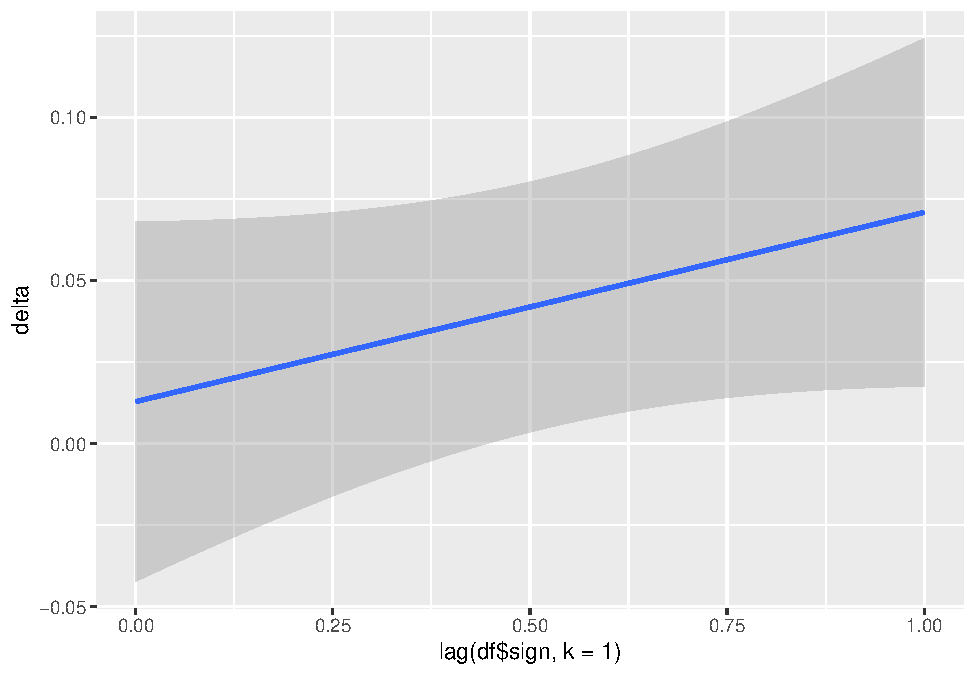
\includegraphics{Econo2_P1_files/figure-latex/lm signt-1} \end{center}

\[\Delta_{t+1} = \alpha + \beta_1 \Delta_t + \beta_2Sign_t + \varepsilon, \hspace{2em} \varepsilon \sim wn(0, \sigma^2)\]

\begin{Shaded}
\begin{Highlighting}[]
\NormalTok{AR1delta <-}\StringTok{ }\KeywordTok{Arima}\NormalTok{(df}\OperatorTok{$}\NormalTok{delta, }\DataTypeTok{order =} \KeywordTok{c}\NormalTok{(}\DecValTok{1}\NormalTok{, }\DecValTok{0}\NormalTok{, }\DecValTok{0}\NormalTok{), }\DataTypeTok{xreg =} \KeywordTok{lag}\NormalTok{(df}\OperatorTok{$}\NormalTok{sign, }
    \DataTypeTok{k =} \DecValTok{1}\NormalTok{))}
\KeywordTok{summary}\NormalTok{(AR1delta)}
\end{Highlighting}
\end{Shaded}

\begin{verbatim}
## Series: df$delta 
## Regression with ARIMA(1,0,0) errors 
## 
## Coefficients:
##          ar1  intercept    xreg
##       0.0321     0.0343  0.0166
## s.e.  0.0306     0.0351  0.0556
## 
## sigma^2 estimated as 0.8219:  log likelihood=-2840.96
## AIC=5689.93   AICc=5689.94   BIC=5712.62
## 
## Training set error measures:
##                        ME      RMSE      MAE MPE MAPE      MASE         ACF1
## Training set 1.147232e-05 0.9059341 0.643417 NaN  Inf 0.7252668 0.0003998294
\end{verbatim}

\begin{Shaded}
\begin{Highlighting}[]
\NormalTok{AR1delta}\OperatorTok{$}\NormalTok{coef[}\DecValTok{1}\NormalTok{]}\OperatorTok{/}\KeywordTok{sqrt}\NormalTok{(AR1delta}\OperatorTok{$}\NormalTok{var.coef[}\DecValTok{1}\NormalTok{, }\DecValTok{1}\NormalTok{])}
\end{Highlighting}
\end{Shaded}

\begin{verbatim}
##     ar1 
## 1.04747
\end{verbatim}

\begin{Shaded}
\begin{Highlighting}[]
\KeywordTok{plot}\NormalTok{(AR1delta)}
\end{Highlighting}
\end{Shaded}

\begin{center}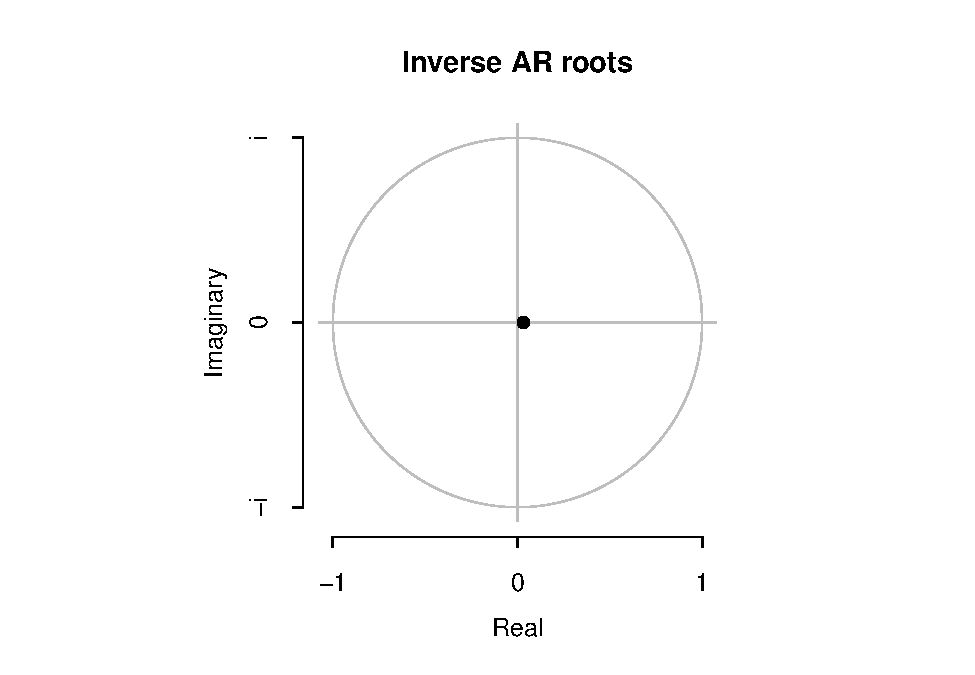
\includegraphics{Econo2_P1_files/figure-latex/delta 1-1} \end{center}

\begin{Shaded}
\begin{Highlighting}[]
\KeywordTok{tsdisplay}\NormalTok{(AR1delta}\OperatorTok{$}\NormalTok{residuals)}
\end{Highlighting}
\end{Shaded}

\begin{center}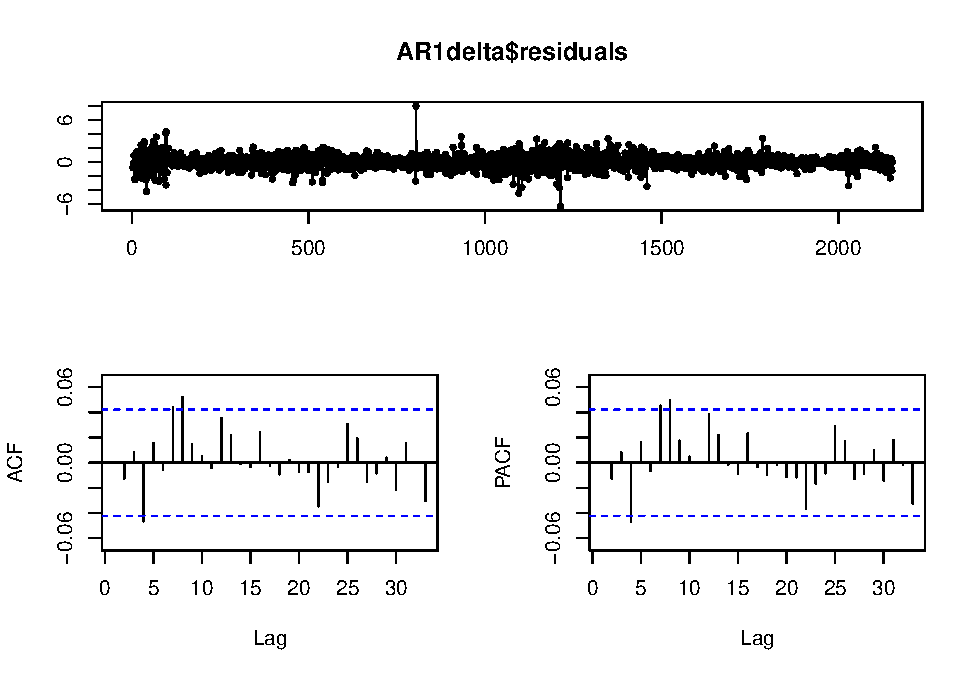
\includegraphics{Econo2_P1_files/figure-latex/delta 1-2} \end{center}

The last hypothesis in the problem refers to the variance:
\[\mathbb{E}(\Delta_{t+1}^2 | \Delta_t).\]

\[\Delta^2_{t+1} = \alpha + \beta \Delta^2_t + \varepsilon, \hspace{2em} \varepsilon \sim wn(0, \sigma^2)\]

\begin{Shaded}
\begin{Highlighting}[]
\NormalTok{AR1var <-}\StringTok{ }\KeywordTok{Arima}\NormalTok{((df}\OperatorTok{$}\NormalTok{delta)}\OperatorTok{^}\DecValTok{2}\NormalTok{, }\DataTypeTok{order =} \KeywordTok{c}\NormalTok{(}\DecValTok{1}\NormalTok{, }\DecValTok{0}\NormalTok{, }\DecValTok{0}\NormalTok{))}
\KeywordTok{summary}\NormalTok{(AR1var)}
\end{Highlighting}
\end{Shaded}

\begin{verbatim}
## Series: (df$delta)^2 
## ARIMA(1,0,0) with non-zero mean 
## 
## Coefficients:
##          ar1    mean
##       0.1701  0.8238
## s.e.  0.0212  0.0582
## 
## sigma^2 estimated as 5.026:  log likelihood=-4792.09
## AIC=9590.17   AICc=9590.18   BIC=9607.2
## 
## Training set error measures:
##                         ME     RMSE       MAE  MPE MAPE      MASE        ACF1
## Training set -6.299133e-05 2.240784 0.9197335 -Inf  Inf 0.8595655 -0.01320252
\end{verbatim}

\begin{Shaded}
\begin{Highlighting}[]
\NormalTok{AR1var}\OperatorTok{$}\NormalTok{coef[}\DecValTok{1}\NormalTok{]}\OperatorTok{/}\KeywordTok{sqrt}\NormalTok{(AR1var}\OperatorTok{$}\NormalTok{var.coef[}\DecValTok{1}\NormalTok{, }\DecValTok{1}\NormalTok{])}
\end{Highlighting}
\end{Shaded}

\begin{verbatim}
##      ar1 
## 8.011092
\end{verbatim}

\begin{Shaded}
\begin{Highlighting}[]
\KeywordTok{plot}\NormalTok{(AR1var)}
\end{Highlighting}
\end{Shaded}

\begin{center}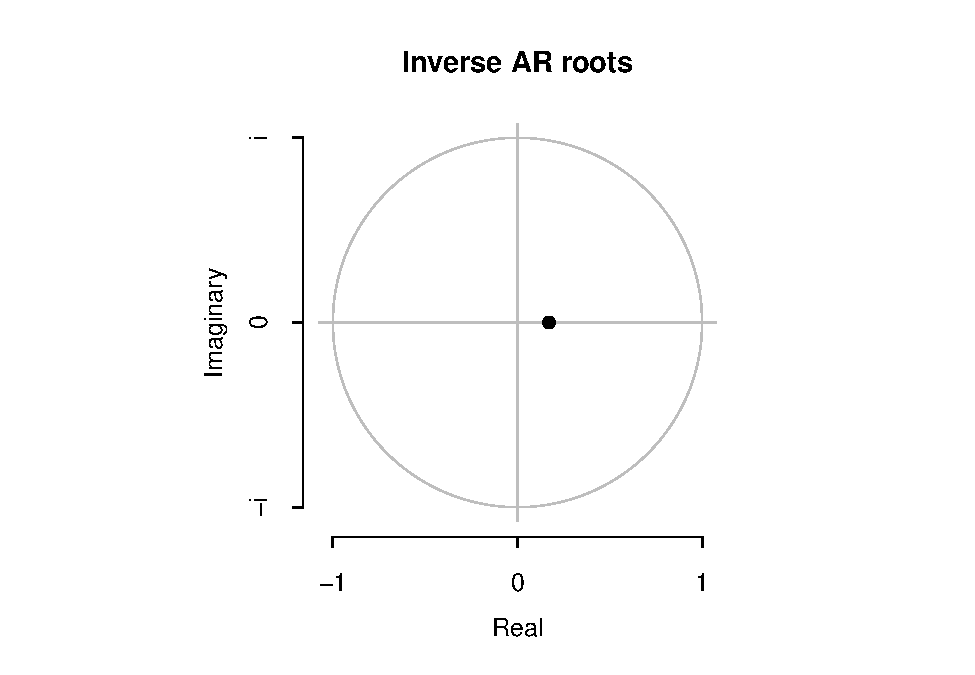
\includegraphics{Econo2_P1_files/figure-latex/var1-1} \end{center}

\begin{Shaded}
\begin{Highlighting}[]
\KeywordTok{tsdisplay}\NormalTok{(AR1var}\OperatorTok{$}\NormalTok{residuals)}
\end{Highlighting}
\end{Shaded}

\begin{center}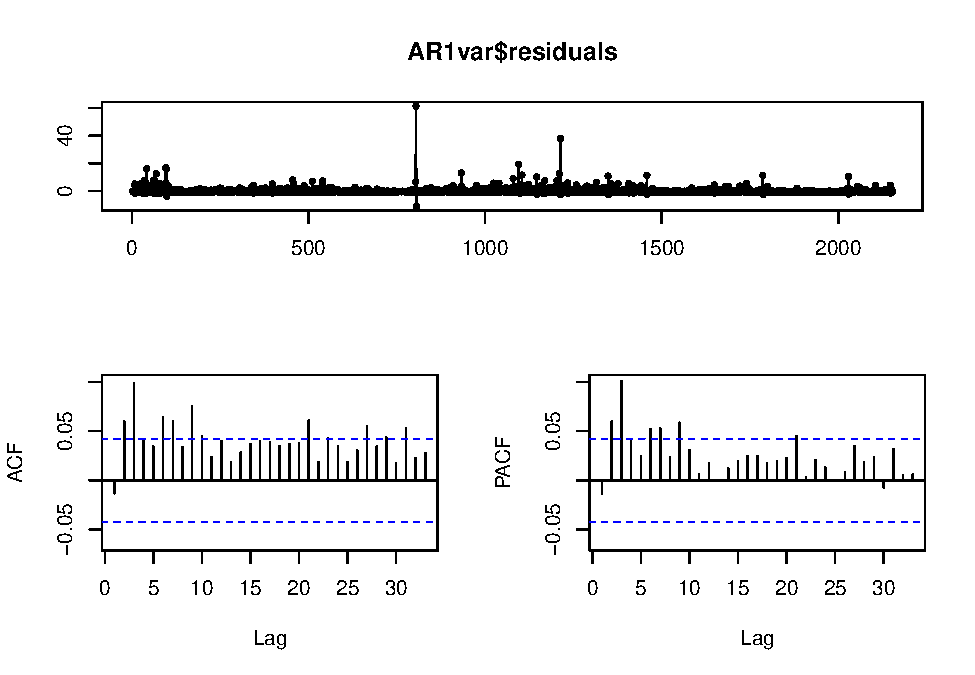
\includegraphics{Econo2_P1_files/figure-latex/var1-2} \end{center}

Now, let's run \emph{auto.arima}.

\begin{Shaded}
\begin{Highlighting}[]
\NormalTok{aadelta <-}\StringTok{ }\KeywordTok{auto.arima}\NormalTok{(df}\OperatorTok{$}\NormalTok{delta, }\DataTypeTok{stepwise =}\NormalTok{ F)}
\KeywordTok{summary}\NormalTok{(aadelta)}
\end{Highlighting}
\end{Shaded}

\begin{verbatim}
## Series: df$delta 
## ARIMA(1,0,1) with non-zero mean 
## 
## Coefficients:
##           ar1     ma1    mean
##       -0.7138  0.7506  0.0433
## s.e.   0.1486  0.1399  0.0199
## 
## sigma^2 estimated as 0.8208:  log likelihood=-2840.87
## AIC=5689.74   AICc=5689.76   BIC=5712.44
## 
## Training set error measures:
##                        ME      RMSE       MAE MPE MAPE    MASE        ACF1
## Training set 2.610156e-05 0.9053381 0.6434199 NaN  Inf 0.72527 0.003320553
\end{verbatim}

\begin{Shaded}
\begin{Highlighting}[]
\KeywordTok{plot}\NormalTok{(aadelta)}
\end{Highlighting}
\end{Shaded}

\begin{center}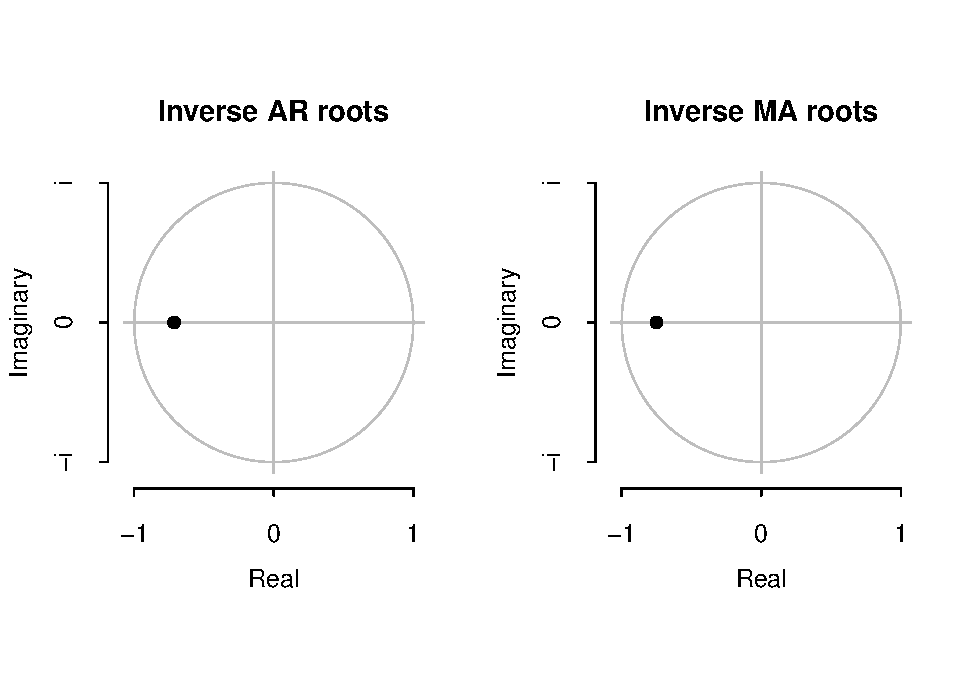
\includegraphics{Econo2_P1_files/figure-latex/auto arima-1} \end{center}

\begin{Shaded}
\begin{Highlighting}[]
\KeywordTok{tsdisplay}\NormalTok{(aadelta}\OperatorTok{$}\NormalTok{residuals)}
\end{Highlighting}
\end{Shaded}

\begin{center}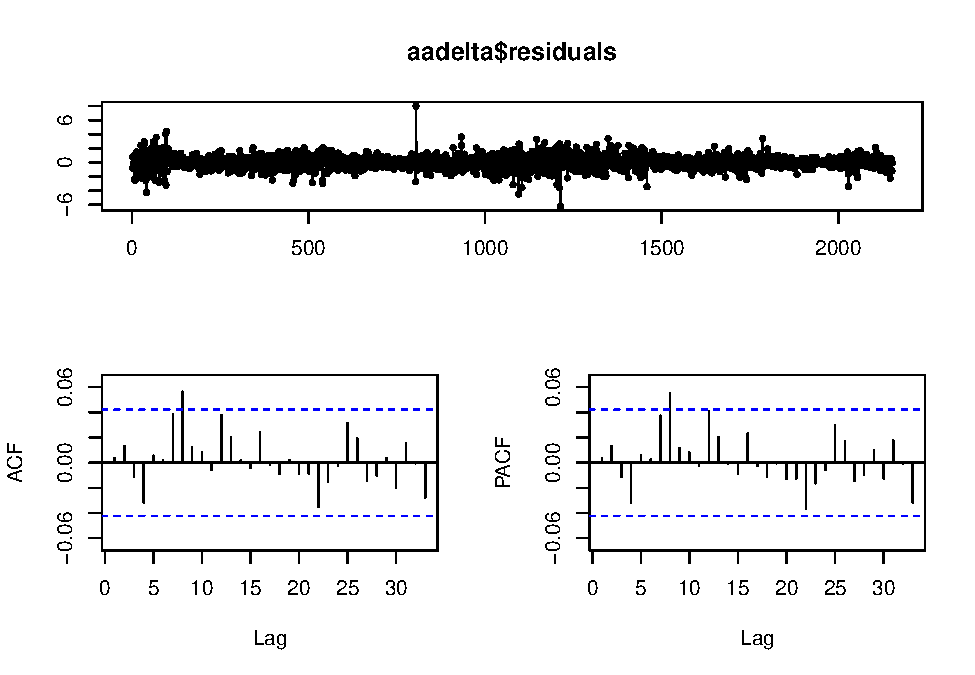
\includegraphics{Econo2_P1_files/figure-latex/auto arima-2} \end{center}

\begin{Shaded}
\begin{Highlighting}[]
\NormalTok{aasign <-}\StringTok{ }\KeywordTok{auto.arima}\NormalTok{(df}\OperatorTok{$}\NormalTok{sign, }\DataTypeTok{stepwise =}\NormalTok{ F)}
\KeywordTok{summary}\NormalTok{(aasign)}
\end{Highlighting}
\end{Shaded}

\begin{verbatim}
## Series: df$sign 
## ARIMA(0,0,0) with non-zero mean 
## 
## Coefficients:
##         mean
##       0.5165
## s.e.  0.0108
## 
## sigma^2 estimated as 0.2498:  log likelihood=-1561.46
## AIC=3126.91   AICc=3126.92   BIC=3138.26
## 
## Training set error measures:
##                         ME      RMSE       MAE  MPE MAPE     MASE       ACF1
## Training set -2.382602e-13 0.4997281 0.4994563 -Inf  Inf 1.028545 0.02773919
\end{verbatim}

\begin{Shaded}
\begin{Highlighting}[]
\KeywordTok{plot}\NormalTok{(aasign)}
\end{Highlighting}
\end{Shaded}

\begin{verbatim}
## Warning in plot.Arima(aasign): No roots to plot
\end{verbatim}

\begin{center}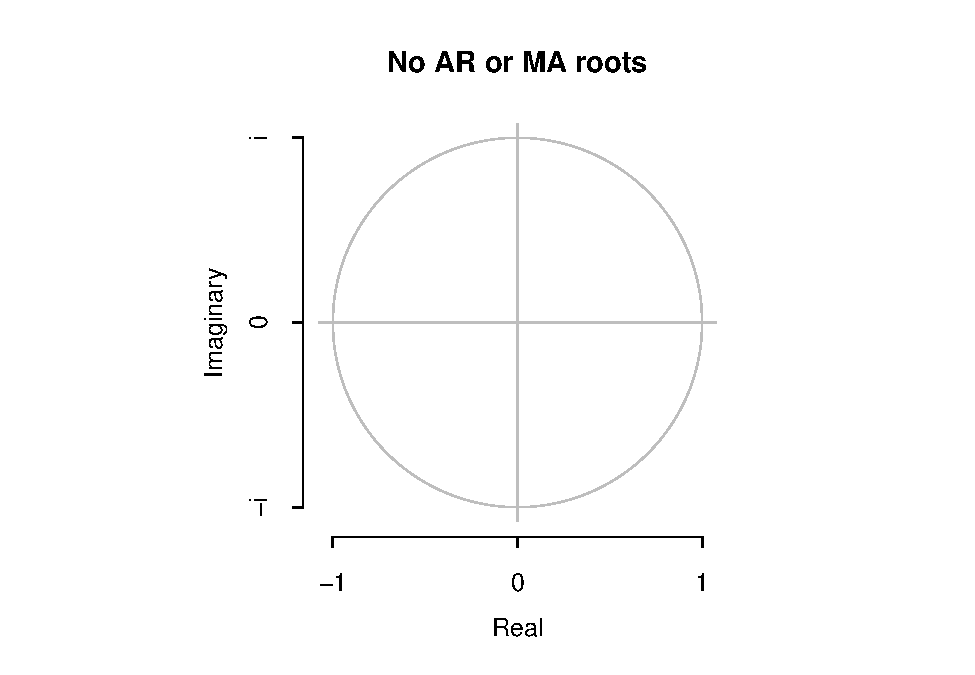
\includegraphics{Econo2_P1_files/figure-latex/auto arima-3} \end{center}

\begin{Shaded}
\begin{Highlighting}[]
\KeywordTok{tsdisplay}\NormalTok{(aasign}\OperatorTok{$}\NormalTok{residuals)}
\end{Highlighting}
\end{Shaded}

\begin{center}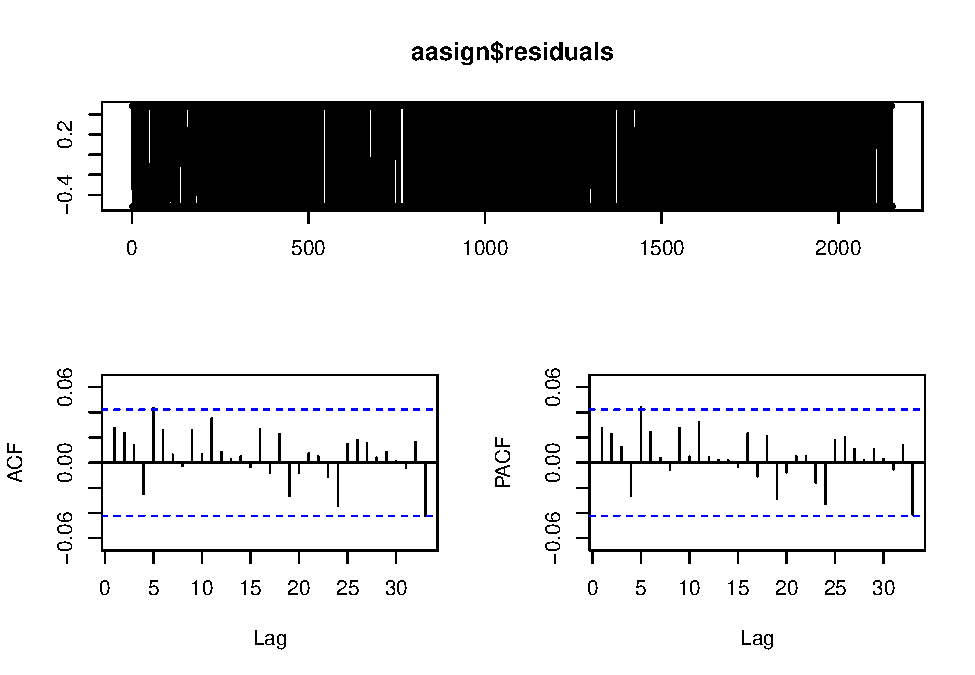
\includegraphics{Econo2_P1_files/figure-latex/auto arima-4} \end{center}

\begin{Shaded}
\begin{Highlighting}[]
\NormalTok{aavar <-}\StringTok{ }\KeywordTok{auto.arima}\NormalTok{((df}\OperatorTok{$}\NormalTok{delta)}\OperatorTok{^}\DecValTok{2}\NormalTok{, }\DataTypeTok{stepwise =}\NormalTok{ F)}
\KeywordTok{summary}\NormalTok{(aavar)}
\end{Highlighting}
\end{Shaded}

\begin{verbatim}
## Series: (df$delta)^2 
## ARIMA(0,1,4) 
## 
## Coefficients:
##           ma1      ma2     ma3      ma4
##       -0.8662  -0.0671  0.0228  -0.0641
## s.e.   0.0215   0.0284  0.0280   0.0214
## 
## sigma^2 estimated as 4.892:  log likelihood=-4761.22
## AIC=9532.45   AICc=9532.48   BIC=9560.82
## 
## Training set error measures:
##                       ME     RMSE       MAE  MPE MAPE      MASE         ACF1
## Training set -0.02170361 2.209213 0.8904046 -Inf  Inf 0.8321553 0.0001189823
\end{verbatim}

\begin{Shaded}
\begin{Highlighting}[]
\KeywordTok{plot}\NormalTok{(aavar)}
\end{Highlighting}
\end{Shaded}

\begin{center}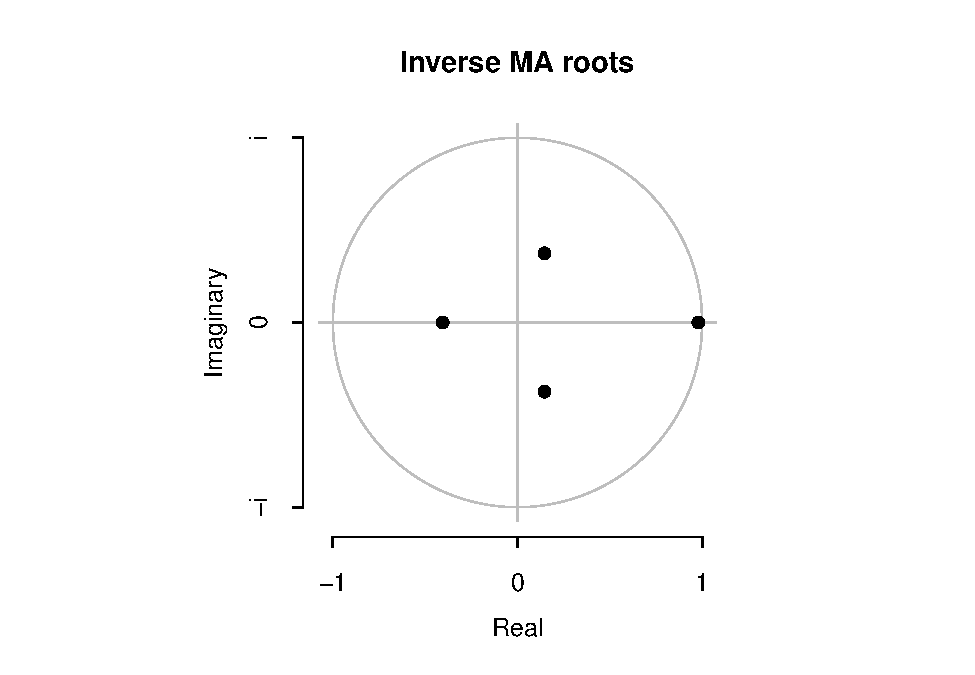
\includegraphics{Econo2_P1_files/figure-latex/auto arima-5} \end{center}

\begin{Shaded}
\begin{Highlighting}[]
\KeywordTok{tsdisplay}\NormalTok{(aasign}\OperatorTok{$}\NormalTok{residuals)}
\end{Highlighting}
\end{Shaded}

\begin{center}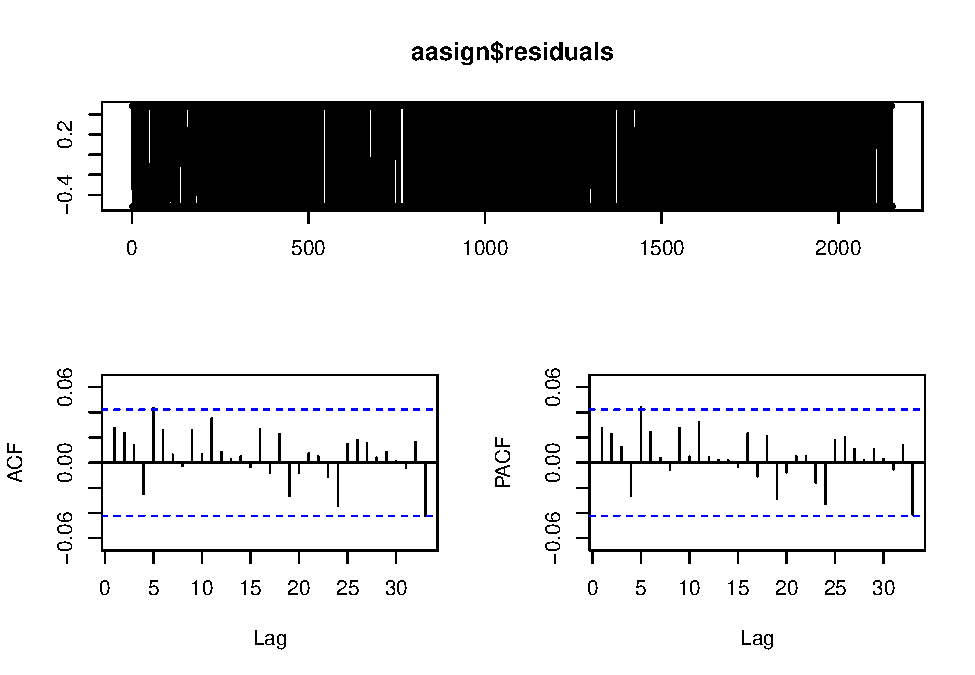
\includegraphics{Econo2_P1_files/figure-latex/auto arima-6} \end{center}

\begin{Shaded}
\begin{Highlighting}[]
\NormalTok{aardelta <-}\StringTok{ }\KeywordTok{auto.arima}\NormalTok{(df}\OperatorTok{$}\NormalTok{delta, }\DataTypeTok{max.q =} \DecValTok{0}\NormalTok{, }\DataTypeTok{stepwise =}\NormalTok{ F)}
\KeywordTok{summary}\NormalTok{(aardelta)}
\end{Highlighting}
\end{Shaded}

\begin{verbatim}
## Series: df$delta 
## ARIMA(1,0,0) with non-zero mean 
## 
## Coefficients:
##          ar1    mean
##       0.0382  0.0433
## s.e.  0.0215  0.0203
## 
## sigma^2 estimated as 0.8215:  log likelihood=-2842.26
## AIC=5690.52   AICc=5690.53   BIC=5707.54
## 
## Training set error measures:
##                         ME      RMSE       MAE MPE MAPE      MASE         ACF1
## Training set -1.464203e-05 0.9059233 0.6434299 NaN  Inf 0.7252813 0.0004805619
\end{verbatim}

\begin{Shaded}
\begin{Highlighting}[]
\KeywordTok{plot}\NormalTok{(aardelta)}
\end{Highlighting}
\end{Shaded}

\begin{center}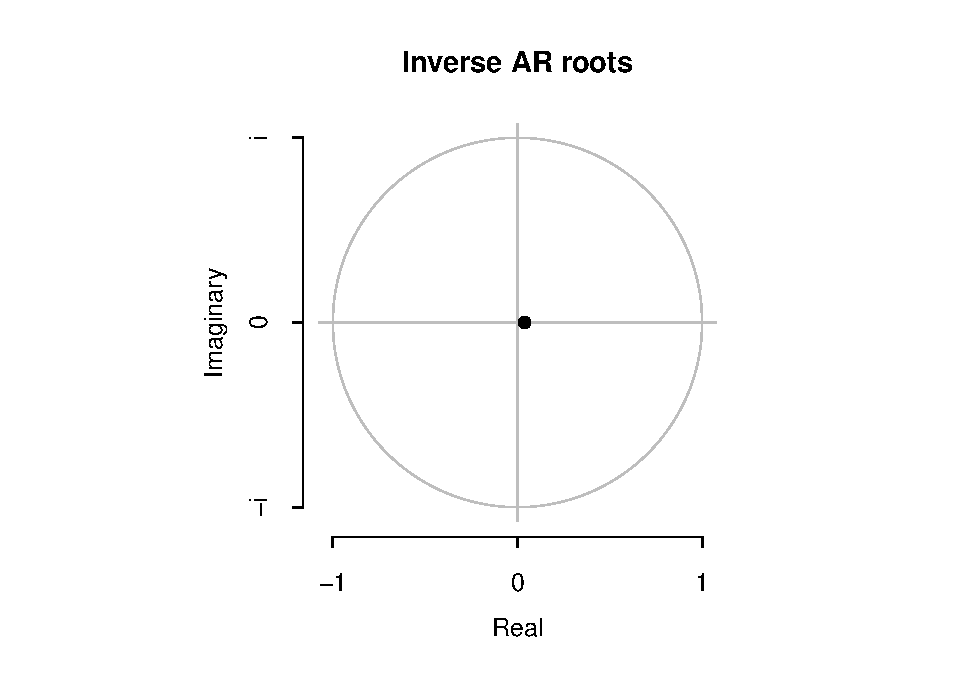
\includegraphics{Econo2_P1_files/figure-latex/auto arima-7} \end{center}

\begin{Shaded}
\begin{Highlighting}[]
\KeywordTok{tsdisplay}\NormalTok{(aardelta}\OperatorTok{$}\NormalTok{residuals)}
\end{Highlighting}
\end{Shaded}

\begin{center}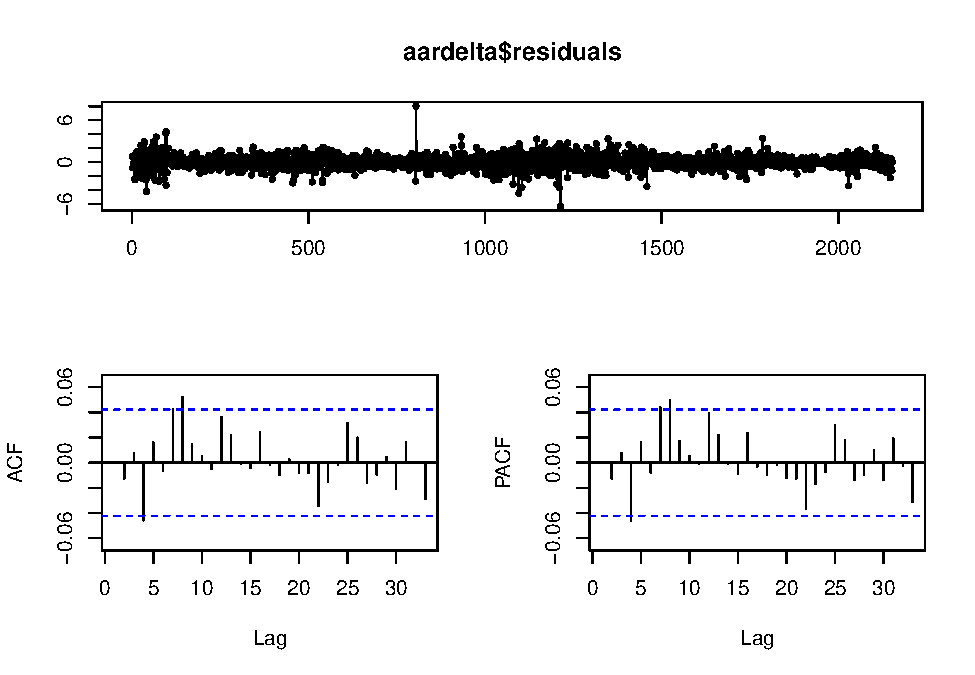
\includegraphics{Econo2_P1_files/figure-latex/auto arima-8} \end{center}

\begin{Shaded}
\begin{Highlighting}[]
\NormalTok{aarsign <-}\StringTok{ }\KeywordTok{auto.arima}\NormalTok{(df}\OperatorTok{$}\NormalTok{sign, }\DataTypeTok{max.q =} \DecValTok{0}\NormalTok{, }\DataTypeTok{stepwise =}\NormalTok{ F)}
\KeywordTok{summary}\NormalTok{(aarsign)}
\end{Highlighting}
\end{Shaded}

\begin{verbatim}
## Series: df$sign 
## ARIMA(0,0,0) with non-zero mean 
## 
## Coefficients:
##         mean
##       0.5165
## s.e.  0.0108
## 
## sigma^2 estimated as 0.2498:  log likelihood=-1561.46
## AIC=3126.91   AICc=3126.92   BIC=3138.26
## 
## Training set error measures:
##                         ME      RMSE       MAE  MPE MAPE     MASE       ACF1
## Training set -2.382602e-13 0.4997281 0.4994563 -Inf  Inf 1.028545 0.02773919
\end{verbatim}

\begin{Shaded}
\begin{Highlighting}[]
\KeywordTok{plot}\NormalTok{(aarsign)}
\end{Highlighting}
\end{Shaded}

\begin{verbatim}
## Warning in plot.Arima(aarsign): No roots to plot
\end{verbatim}

\begin{center}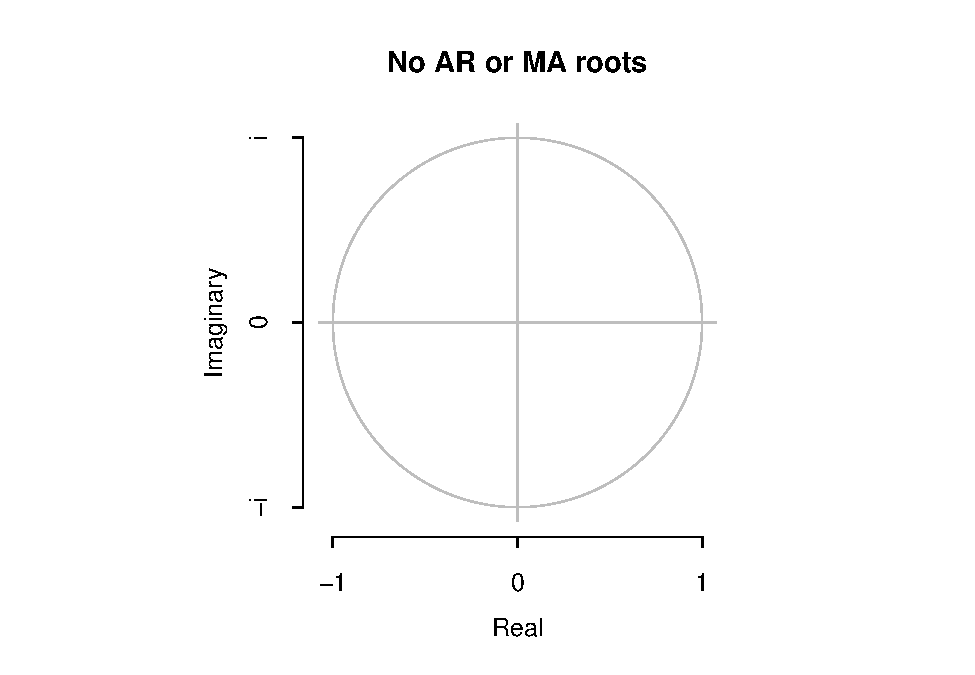
\includegraphics{Econo2_P1_files/figure-latex/auto arima-9} \end{center}

\begin{Shaded}
\begin{Highlighting}[]
\KeywordTok{tsdisplay}\NormalTok{(aarsign}\OperatorTok{$}\NormalTok{residuals)}
\end{Highlighting}
\end{Shaded}

\begin{center}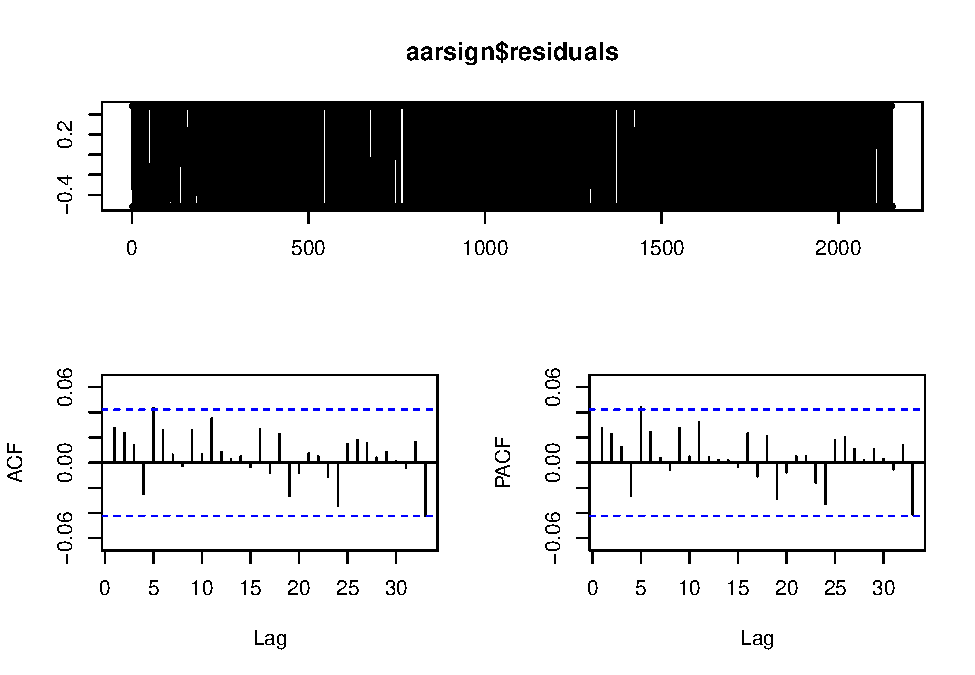
\includegraphics{Econo2_P1_files/figure-latex/auto arima-10} \end{center}

\begin{Shaded}
\begin{Highlighting}[]
\NormalTok{aarvar <-}\StringTok{ }\KeywordTok{auto.arima}\NormalTok{((df}\OperatorTok{$}\NormalTok{delta)}\OperatorTok{^}\DecValTok{2}\NormalTok{, }\DataTypeTok{max.q =} \DecValTok{0}\NormalTok{, }\DataTypeTok{stepwise =}\NormalTok{ F)}
\KeywordTok{summary}\NormalTok{(aarvar)}
\end{Highlighting}
\end{Shaded}

\begin{verbatim}
## Series: (df$delta)^2 
## ARIMA(5,1,0) 
## 
## Coefficients:
##           ar1      ar2      ar3      ar4      ar5
##       -0.7420  -0.5845  -0.4042  -0.2873  -0.1687
## s.e.   0.0213   0.0259   0.0274   0.0258   0.0212
## 
## sigma^2 estimated as 5.465:  log likelihood=-4878.95
## AIC=9769.89   AICc=9769.93   BIC=9803.94
## 
## Training set error measures:
##                         ME     RMSE       MAE  MPE MAPE      MASE       ACF1
## Training set -3.234587e-05 2.334504 0.9170278 -Inf  Inf 0.8570369 -0.0239684
\end{verbatim}

\begin{Shaded}
\begin{Highlighting}[]
\KeywordTok{plot}\NormalTok{(aarvar)}
\end{Highlighting}
\end{Shaded}

\begin{center}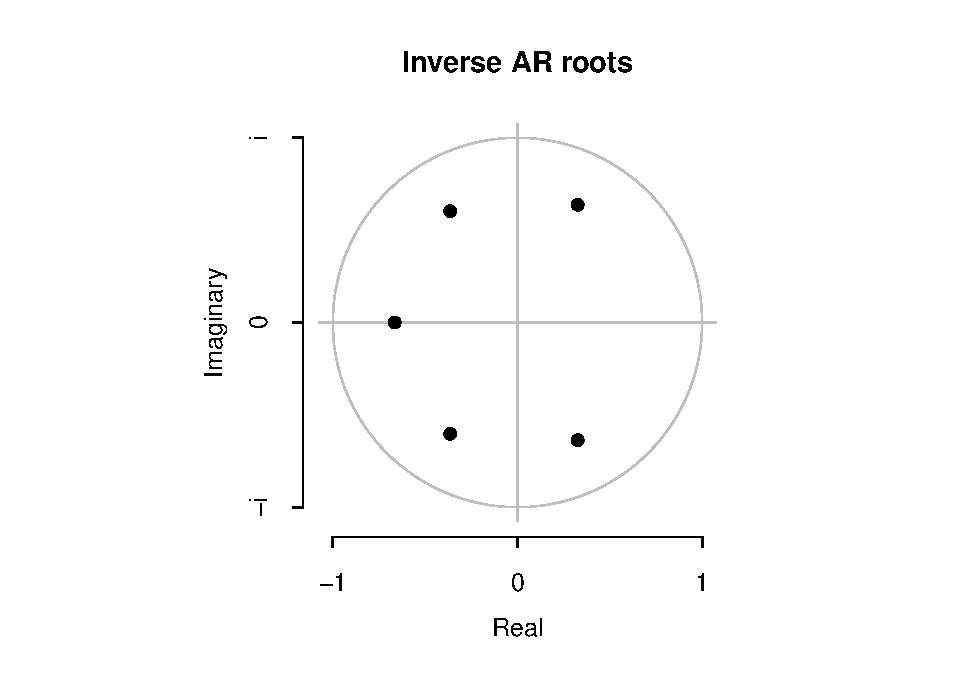
\includegraphics{Econo2_P1_files/figure-latex/auto arima-11} \end{center}

\begin{Shaded}
\begin{Highlighting}[]
\KeywordTok{tsdisplay}\NormalTok{(aarvar}\OperatorTok{$}\NormalTok{residuals)}
\end{Highlighting}
\end{Shaded}

\begin{center}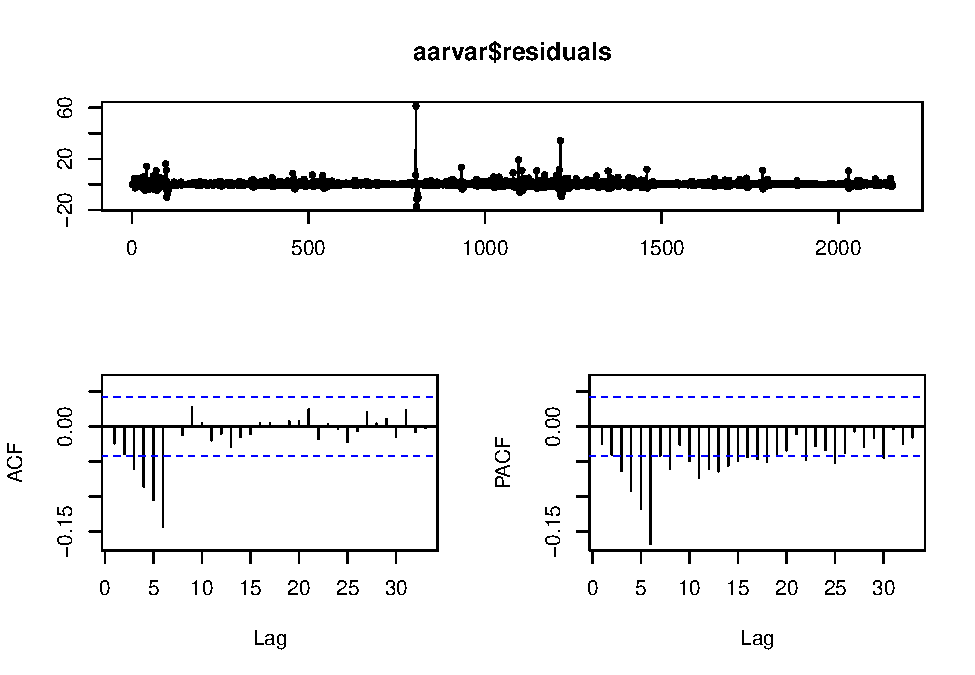
\includegraphics{Econo2_P1_files/figure-latex/auto arima-12} \end{center}

\[ \Delta_{t+1} = c + \beta \Delta_t + \varepsilon\]

\begin{Shaded}
\begin{Highlighting}[]
\NormalTok{AR1_}\DecValTok{2}\NormalTok{ <-}\StringTok{ }\KeywordTok{Arima}\NormalTok{(df}\OperatorTok{$}\NormalTok{delta, }\DataTypeTok{order =} \KeywordTok{c}\NormalTok{(}\DecValTok{1}\NormalTok{, }\DecValTok{0}\NormalTok{, }\DecValTok{0}\NormalTok{))}

\KeywordTok{summary}\NormalTok{(AR1_}\DecValTok{2}\NormalTok{)}
\end{Highlighting}
\end{Shaded}

\begin{verbatim}
## Series: df$delta 
## ARIMA(1,0,0) with non-zero mean 
## 
## Coefficients:
##          ar1    mean
##       0.0382  0.0433
## s.e.  0.0215  0.0203
## 
## sigma^2 estimated as 0.8215:  log likelihood=-2842.26
## AIC=5690.52   AICc=5690.53   BIC=5707.54
## 
## Training set error measures:
##                         ME      RMSE       MAE MPE MAPE      MASE         ACF1
## Training set -1.464203e-05 0.9059233 0.6434299 NaN  Inf 0.7252813 0.0004805619
\end{verbatim}

\begin{Shaded}
\begin{Highlighting}[]
\KeywordTok{confint}\NormalTok{(AR1_}\DecValTok{2}\NormalTok{, }\DataTypeTok{level =} \FloatTok{0.95}\NormalTok{)}
\end{Highlighting}
\end{Shaded}

\begin{verbatim}
##                  2.5 %     97.5 %
## ar1       -0.003988796 0.08042284
## intercept  0.003511958 0.08308440
\end{verbatim}


\chapter{Problem 2: Estimating ARMA models} \label{Problem-2}

Consider an ARMA($\cdot$) model of the form:
$$
\begin{aligned}
Y_{t}=& C+\phi_{1} Y_{t-1}+\phi Y_{t-2}+\cdots+\phi_{P} Y_{t-p}+\varepsilon_{t} \\
&+\theta_{1} \varepsilon_{t-1}+\theta_{2} \varepsilon_{t-2}+\cdots+\theta_{q} \varepsilon_{t-q}
\end{aligned}
$$
with white noise $\varepsilon_{+}$:
$$
\begin{aligned}
\mathbb{E}\left(\varepsilon_{t}\right) &=0 \\
E\left(\varepsilon_{t} \varepsilon_{\tau}\right) &=\left\{\begin{array}{ll}
\sigma^{2}, & \forall t=\tau \\
0, & c \cdot c
\end{array}\right.
\end{aligned}
$$

We'll use MLE, with $\Theta = (c, \phi_1, ..., \phi_p, \theta_1, ..., \theta_q)'$ a vector of parameters. This means that we need to calculate the pdf: $f_{Y_T, Y_{T-1},...}(y_T, y_{T-1},...; \Theta)$. We usually assume a normal distribution for $\varepsilon$.

\section{MLE for Gaussian AR(1)}
$$ Y_t = c + \phi Y_{t-1} + \varepsilon_{t}, \hspace{1em} (\Theta = (c, \theta, \sigma^2)') $$
$$ \mathbb{E}(Y_1) = \mu = \dfrac{c}{1- \phi}$$
$$ \mathbb{E}(Y_1 - \mu)^2 = \dfrac{\sigma^2}{1 - \phi^2} $$ 

The likelihood function is given by: 
$$f_{Y_1}(y_1; \Theta) * \Pi_{t=2}^T f_{Y_t| Y_{t-1}}(y_t | y_{t-1}; \Theta)$$ 
$$ \mathcal{L}(\Theta) = log \, f_{Y_1}(y_1; \Theta) + \sum_{t=2}^T log \, f_{Y_t| Y_{t-1}}(y_t | y_{t-1}; \Theta) $$

\subsection{Conditional MLE}

$$ \Pi_{t=2}^T f_{Y_t| Y_{t-1}}(y_t | y_{t-1}; \Theta) $$

For the gaussian case, the minimization problem is equivalent to minimizing:
$$ \sum_{t=2}^T (y_t - c - \phi y_{t-1})^2$$ 
This means that the \textit{conditional MLE is equivalent to OLS!}

\section{Likelihood funciton for AR(p)}

$$
Y_t = c + \phi_1 Y_{t-1} + ... + \phi_p Y_{t-p} + \varepsilon_{t}, \hspace{1em} \varepsilon_{t} \sim wn(0, \sigma^2), \hspace{1em} \Theta = (c, \phi_1, ..., \phi_p, \sigma^2) $$
$$ \mu = \dfrac{c}{1 - \phi_{1} - ... - \phi_{p}} $$
$$ \sigma^2 V_p \text{is the var-cov matrix}$$
$$ f_{Y_p, Y_{p-1},...}(y_p, y_{p-1},...; \Theta) * \Pi_{t = p+1}^T f_{Y_t | Y_{t-1, ..., Y_{t-p}}} (y_t | y_{t-1}, ..., y_{t-p}; \Theta)$$ 

The first term represents the distribution of the $p$ first observations. The second term is the \textit{prediction error decomposition.}

\subsection{Conditional MLE}

Again, we can apply traditional OLS estimation in the conditional MLE case, because it minimizes:
$$ \sum_{t = p+1}^T (Y_t - c - \phi_1 Y_{t-1} - ... - \phi_p Y_{t-p})^2 $$
Thus, the variance estimator is also the one that we are used to: 
$$\hat{\sigma}^{2}=\frac{1}{T-p} \sum_{t=p+1}^{T}\left(y_{t}-\hat{c}-\hat{\phi}_{1} y_{t-1}-\cdots-\hat{\phi}_{p} y_{t-p}\right)^{2}$$

\section{MLE for Gaussian MA($\cdot$)}

Let's now begin with the Conditional MLE. 
$$ Y_t = \mu + \theta \varepsilon_{t-1} + \varepsilon_{t}, \hspace{1em} \varepsilon_{t} \sim wn(0, \sigma^2), \hspace{1em} \Theta = (\mu, \theta, \sigma^2) $$
$$ \mathcal{L}(\Theta) = log \, f_{Y_t, Y_{t-1},..., Y_1 | \varepsilon_0 = 0} (y_T, y_{T-1}, ..., y_1 | \varepsilon_{0} = 0; \Theta) $$ 
$$ \mathcal{L}(\Theta) = -\dfrac{T}{2} log \, (2 \pi) - \dfrac{T}{2} log \, (\sigma^2) - \sum_{t=1}^T \dfrac{\varepsilon_{t}^2}{2 \sigma^2} $$

If $| \theta | < 1$, the effects of imposing $\varepsilon_0 = 0$ diminish over time and the conditional MLE is a good approximation. Otherwise, it is not -- the effects build up over time. This is why an essential condition for an ARMA(p,q) model is \textit{invertibility.}

The same idea can be generalized for an MA(q) model. If we fix the first $q$ values of $\varepsilon$ as 0: $ \varepsilon_0 = \varepsilon_{-1} = ... = \varepsilon_{-q+1} = 0$, we can iterate on the values of the innovation terms:
$$ \varepsilon_t = y_t - \mu - \theta_1 \varepsilon_{t-1} - ... - \theta_q \varepsilon_{t-q}. $$

\section{Conditional MLE estimation for ARMA(p,q) models}

Uniting both of the results shown above, we can apply conditional MLE estimation for an ARMA(p,q) model:
$$ Y_t = c + \phi Y_{t-1} + ... + \phi_p Y_{t-p} + \theta_1 \varepsilon_{t-1} + ... + \theta_q \varepsilon_{t-q} + \varepsilon_t, \hspace{1em} \varepsilon_t \sim wn(0, \sigma^2) $$

This is possible by taking fixed initial values for $y_0 = (y_0, ..., y_{-p+1})', \varepsilon_0 = (\varepsilon_0, ..., \varepsilon_{-q+1})'$ as given. Then, we apply the log-likelihood function:
$$ \mathcal{L} (\Theta) = -\dfrac{T}{2} log \, (2\pi) -\dfrac{T}{2} log \, (\sigma^2) - \sum_{t=1}^{T} \dfrac{\varepsilon_t^2}{2 \sigma^2}$$


\chapter{Problem 3: Identification of ARMA models}

In this problem, we'll be tackling the issue of \emph{identification} of
an ARMA model. Namely, we will employ the \emph{Box-Jenkins} model
selection strategy, based upon the concept of \emph{parsimony}.

The principle of \emph{parsimony} is inspired on the trade-off between
\emph{fit}, i.e., \(R^2\), and \emph{degrees of freedom}. ``Box and
Jenkins argue that parsimonious models produce better forecasts than
overparametrized models''. (p.~76)

The Box-Jenkins strategy is divided in three main stages:

\begin{itemize}
	\item Identification;
	\item Estimation;
	\item Diagnostic checking.
\end{itemize}

These estimations depend upon two essential conditions (discussed in
earlier problems and lectures): \emph{stationarity} and
\emph{invertibility}. Stationarity, as we have discussed earlier, is
necessary to effectively \emph{employ econometric methods} and to infer
characteristics of a population through a given sample. Enders also
points out that t-statistics and Q-statistics are based upon the
assumption that the data are stationary (p.~77). This implies a
condition on the \emph{AR} process of an ARMA model (roots of
characteristic polynomial outside of unity circle).

Furthermore, the model shall be \emph{invertible} -- i.e., if it can be
represented by a finite or convergent AR model. This implies a condition
on the \emph{MA} process -- i.e., if it can be written as an
AR(\(\infty\)).

We're going to check these conditions intuitively by plotting the ACFs
and PACFs of the time series:

\begin{Shaded}
	\begin{Highlighting}[]
		\NormalTok{df <-}\StringTok{ }\KeywordTok{data.frame}\NormalTok{(df)}
		
		\NormalTok{pplot <-}\StringTok{ }\KeywordTok{ggplot}\NormalTok{(}\DataTypeTok{data =}\NormalTok{ df, }\KeywordTok{aes}\NormalTok{(}\DataTypeTok{x =}\NormalTok{ t, }\DataTypeTok{y =}\NormalTok{ value)) }\OperatorTok{+}\StringTok{ }\KeywordTok{geom_line}\NormalTok{() }\OperatorTok{+}\StringTok{ }
		\StringTok{    }\KeywordTok{ggtitle}\NormalTok{(}\StringTok{"Time series plot"}\NormalTok{) }\OperatorTok{+}\StringTok{ }\KeywordTok{theme_few}\NormalTok{()}
		\NormalTok{pplot}
	\end{Highlighting}
\end{Shaded}

\begin{center}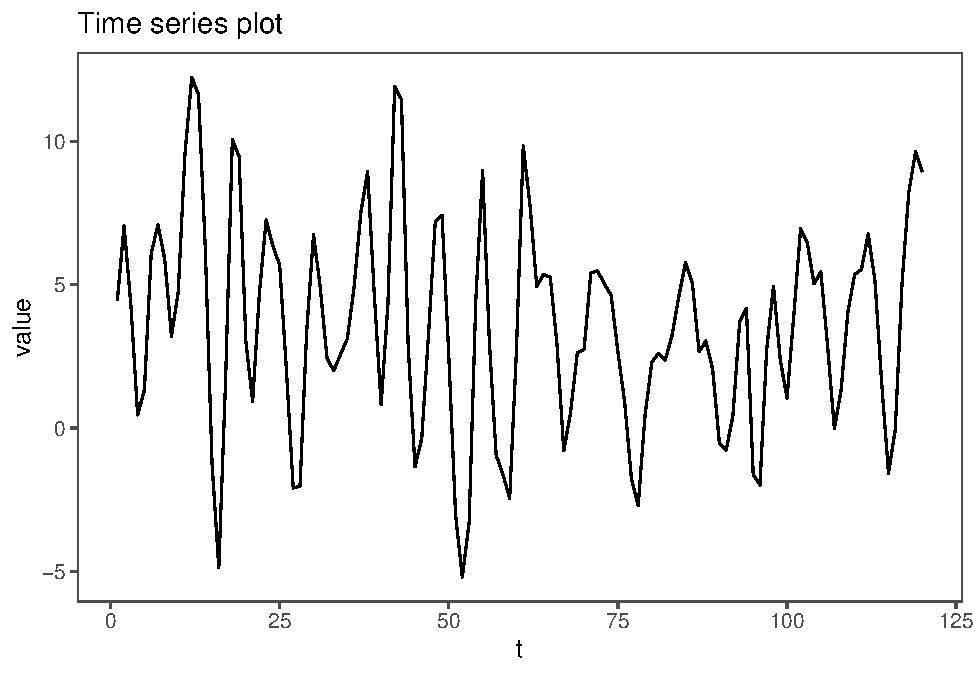
\includegraphics{Econo2_P3_files/figure-latex/plots-1} \end{center}

\begin{Shaded}
	\begin{Highlighting}[]
		\NormalTok{acf_ts <-}\StringTok{ }\KeywordTok{Acf}\NormalTok{(df}\OperatorTok{$}\NormalTok{value, }\DataTypeTok{lag.max =} \DecValTok{5000}\NormalTok{)}
	\end{Highlighting}
\end{Shaded}

\begin{center}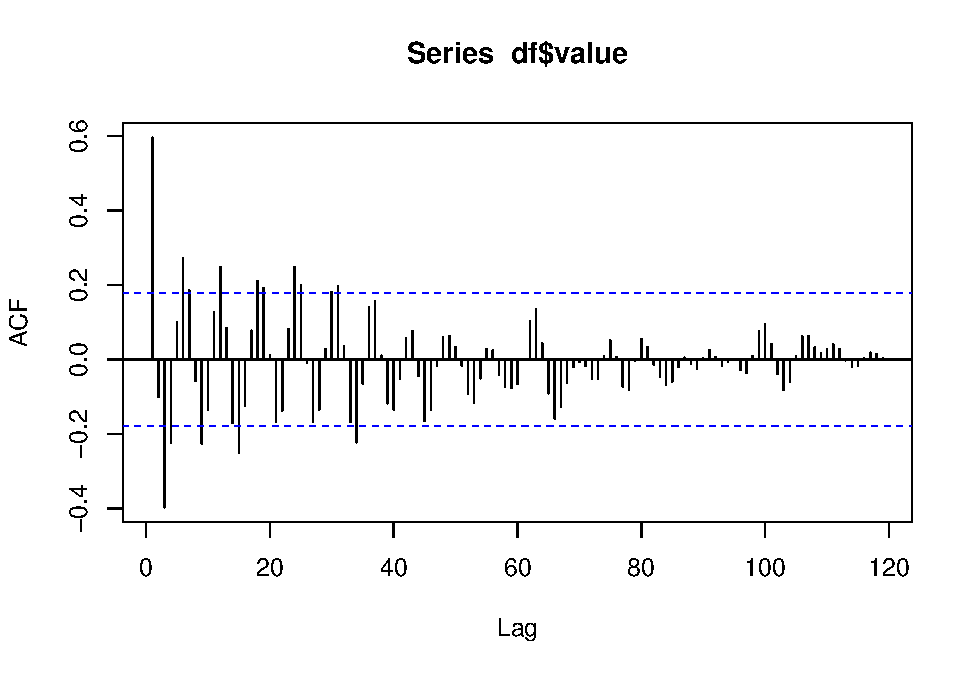
\includegraphics{Econo2_P3_files/figure-latex/plots-2} \end{center}

\begin{Shaded}
	\begin{Highlighting}[]
		\NormalTok{acf_test_values <-}\StringTok{ }\NormalTok{acf_ts}\OperatorTok{$}\NormalTok{acf}\OperatorTok{/}\KeywordTok{sd}\NormalTok{(acf_ts}\OperatorTok{$}\NormalTok{acf)}
		
		\KeywordTok{head}\NormalTok{(}\KeywordTok{data.frame}\NormalTok{(acf_test_values))}
	\end{Highlighting}
\end{Shaded}

\begin{verbatim}
	##   acf_test_values
	## 1       6.5814152
	## 2       3.9180772
	## 3      -0.6619326
	## 4      -2.6109255
	## 5      -1.4713722
	## 6       0.6589976
\end{verbatim}

\begin{Shaded}
	\begin{Highlighting}[]
		\NormalTok{facst <-}\StringTok{ }\KeywordTok{ggAcf}\NormalTok{(df}\OperatorTok{$}\NormalTok{value, }\DataTypeTok{type =} \StringTok{"correlation"}\NormalTok{, }\DataTypeTok{lag.max =} \DecValTok{20}\NormalTok{, }
		\DataTypeTok{plot =}\NormalTok{ T) }\OperatorTok{+}\StringTok{ }\KeywordTok{theme_few}\NormalTok{()}
		\NormalTok{faclt <-}\StringTok{ }\KeywordTok{ggAcf}\NormalTok{(df}\OperatorTok{$}\NormalTok{value, }\DataTypeTok{type =} \StringTok{"correlation"}\NormalTok{, }\DataTypeTok{lag.max =} \DecValTok{5000}\NormalTok{, }
		\DataTypeTok{plot =}\NormalTok{ T) }\OperatorTok{+}\StringTok{ }\KeywordTok{theme_few}\NormalTok{()}
		
		\NormalTok{facpst <-}\StringTok{ }\KeywordTok{ggPacf}\NormalTok{(df}\OperatorTok{$}\NormalTok{value, }\DataTypeTok{type =} \StringTok{"correlation"}\NormalTok{, }\DataTypeTok{lag.max =} \DecValTok{100}\NormalTok{, }
		\DataTypeTok{plot =}\NormalTok{ T) }\OperatorTok{+}\StringTok{ }\KeywordTok{theme_few}\NormalTok{()}
	\end{Highlighting}
\end{Shaded}

\begin{verbatim}
	## Warning: Ignoring unknown parameters: type
\end{verbatim}

\begin{Shaded}
	\begin{Highlighting}[]
		\NormalTok{facplt <-}\StringTok{ }\KeywordTok{ggPacf}\NormalTok{(df}\OperatorTok{$}\NormalTok{value, }\DataTypeTok{type =} \StringTok{"correlation"}\NormalTok{, }\DataTypeTok{lag.max =} \DecValTok{5000}\NormalTok{, }
		\DataTypeTok{plot =}\NormalTok{ T) }\OperatorTok{+}\StringTok{ }\KeywordTok{theme_few}\NormalTok{()}
	\end{Highlighting}
\end{Shaded}

\begin{verbatim}
	## Warning: Ignoring unknown parameters: type
\end{verbatim}

\begin{Shaded}
	\begin{Highlighting}[]
		\NormalTok{facst}
	\end{Highlighting}
\end{Shaded}

\begin{center}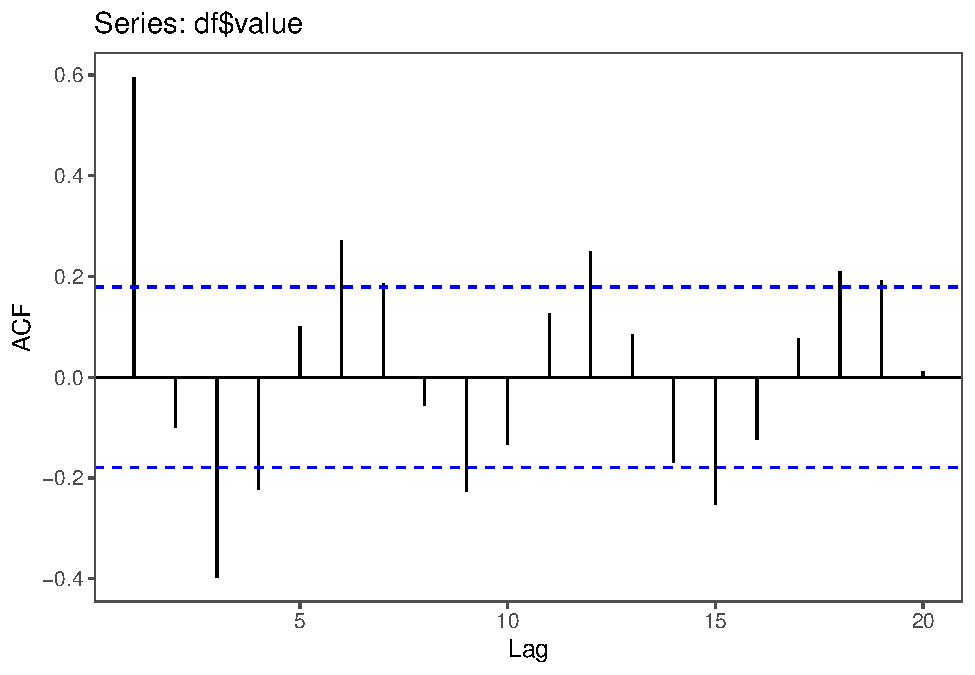
\includegraphics{Econo2_P3_files/figure-latex/plots-3} \end{center}

\begin{Shaded}
	\begin{Highlighting}[]
		\NormalTok{faclt}
	\end{Highlighting}
\end{Shaded}

\begin{center}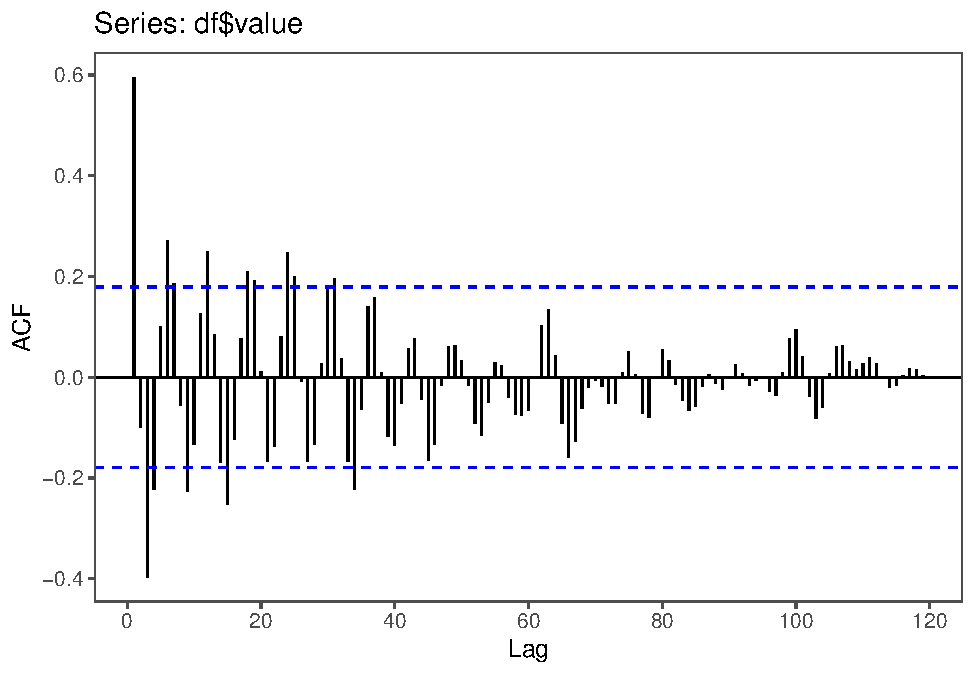
\includegraphics{Econo2_P3_files/figure-latex/plots-4} \end{center}

\begin{Shaded}
	\begin{Highlighting}[]
		\NormalTok{facpst}
	\end{Highlighting}
\end{Shaded}

\begin{center}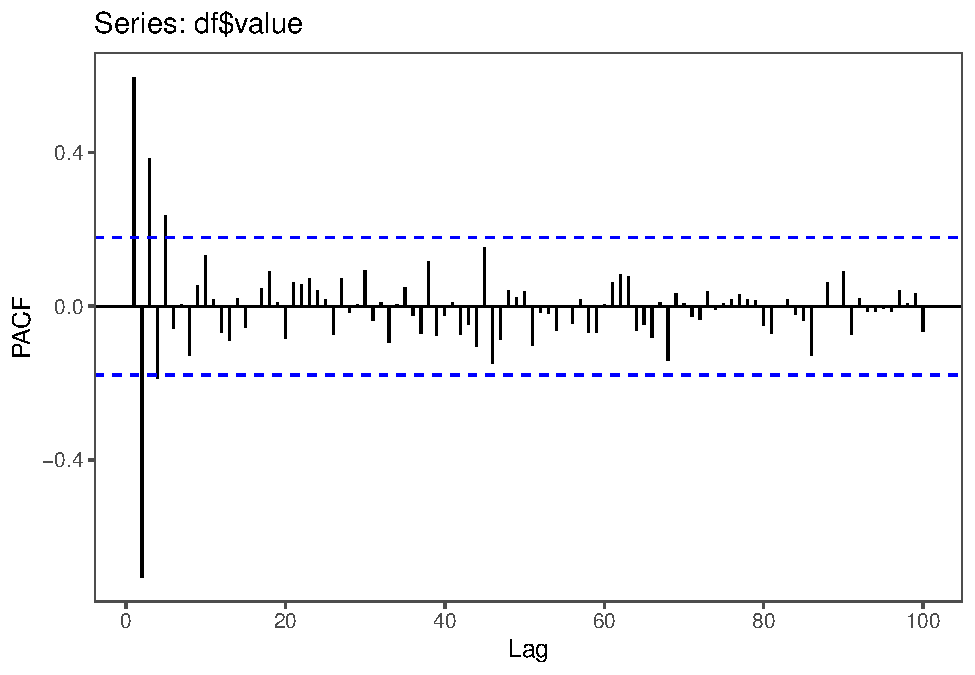
\includegraphics{Econo2_P3_files/figure-latex/plots-5} \end{center}

\begin{Shaded}
	\begin{Highlighting}[]
		\NormalTok{facplt}
	\end{Highlighting}
\end{Shaded}

\begin{center}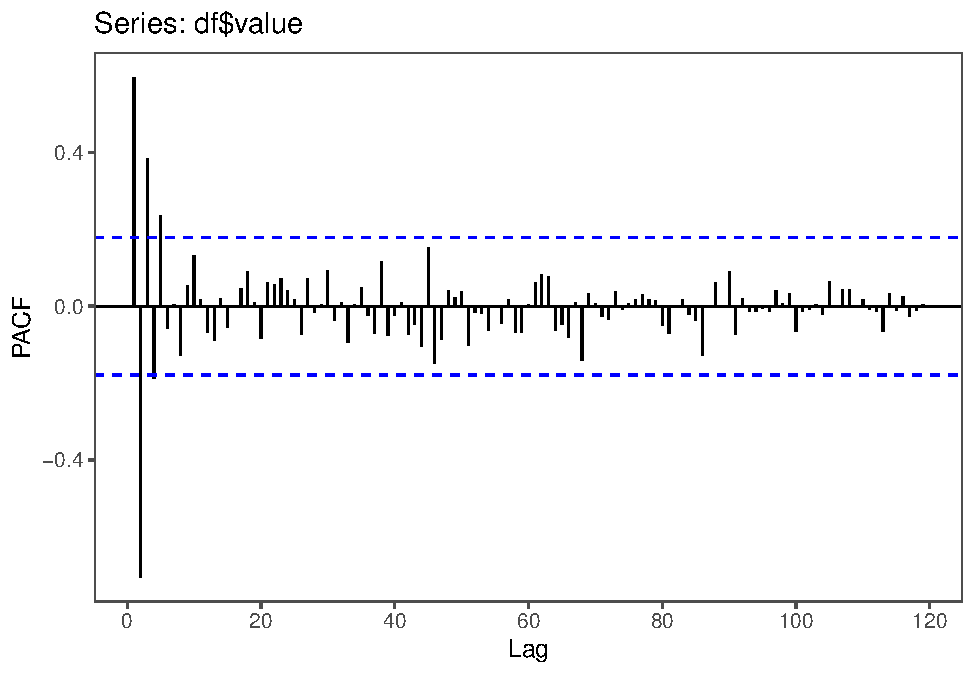
\includegraphics{Econo2_P3_files/figure-latex/plots-6} \end{center}

Aside from usual methods, we'll employ the following criteria:

\begin{itemize}
	\item Akaike Information Criterion (AIC). 
	$$ AIC = T * ln(SSR) + 2n $$
	\item  Schwartz Bayesian Criterion (SBC).
	$$ SBC = T * ln(SSR) + n * ln(T) $$
\end{itemize}

\(n\) denotes the number of parameters estimated (an useful metric given
the importance of the degrees of freedom). \(T\) denotes the number of
\emph{usable} observations. Note that, when comparing different models,
it is important to \emph{fix} \(T\) to ensure that the \(AIC\) and
\(SBC\) values are comparable and are capturing only variations in the
actual model and not the effect of changing T.

The objective with these criteria is to \emph{minimize} their values.
``As the fit of the model improves, the AIC and SBC will approach
-\(\infty\).'' (p.~70) \(AIC\) and \(SBC\) have different advantages and
drawbacks: while the former is biased toward overparametrization and
more powerful in small samples, \(SBC\) is consistent and has superior
large sample properties. If both metrics point to the same model, we
should be fairly confident that it is, indeed, the correct
specification.

It is also important to apply hypothesis tests to the estimates of the
population parameters \(\mu, \sigma^2\) and \(\rho_s\) --
\(\bar{y}, \hat{sigma}^2, r_s\), respectively. Worthy of note here is
\(r_s\), which presents the following distributions under the null that
\(y_t\) is stationary with \(\varepsilon_t \sim \mathcal{N}\):
\[ Var(r_s) = T^{-1} \hspace{2em} for \, s = 1\]
\[ Var(r_s) = T^{-1}(1 + 2\sum_{j=1}^{s-1} r_j^2) \hspace{2em} for \, s > 1\]

The Q-statistic is also introduced by Enders in this chapter. It is used
to test whether a group of autocorrelations is significantly different
from zero. \[Q = T\sum_{k=1}^s r_k^2\] Under the null of
\(r_k = 0 \forall k\), Q is asymptotically \(\chi^2\) with s degrees of
freedom. ``Certainly, a white-noise process (in which all
autocorrelations should be zero) would have a Q value of zero''. (p.~68)

An alternative form for \(Q\) is presented by Ljung and Box (1978):
\[ Q = T(T+2) \sum_{k=1}^s \dfrac{r_k^2}{(T-k)} \]

Furthermore, it is also important to check whether the residuals of the
model are actually \emph{white noise}. This can be done via the
Q-statistic, which \emph{should not result in the rejection of the
	null}. If that is not the case, the model specified is not the best one
available, as there's still a relevant underlying variable (\(y\) or
\(\varepsilon\)).

Let's now perform the \emph{estimation stage}. This shall be done via
the function \emph{auto.arima} from the package \emph{forecast}.

\begin{Shaded}
	\begin{Highlighting}[]
		\NormalTok{aa_model <-}\StringTok{ }\KeywordTok{auto.arima}\NormalTok{(df}\OperatorTok{$}\NormalTok{value, }\DataTypeTok{num.cores =} \DecValTok{24}\NormalTok{, }\DataTypeTok{max.d =} \DecValTok{0}\NormalTok{, }\DataTypeTok{max.D =} \DecValTok{0}\NormalTok{, }
		\DataTypeTok{stepwise =}\NormalTok{ F)}
		
		\KeywordTok{summary}\NormalTok{(aa_model)}
	\end{Highlighting}
\end{Shaded}

\begin{verbatim}
	## Series: df$value 
	## ARIMA(2,0,1) with non-zero mean 
	## 
	## Coefficients:
	##          ar1      ar2    ma1    mean
	##       0.7524  -0.5545  0.797  3.5305
	## s.e.  0.0818   0.0813  0.064  0.3485
	## 
	## sigma^2 estimated as 3.002:  log likelihood=-235.87
	## AIC=481.75   AICc=482.27   BIC=495.68
	## 
	## Training set error measures:
	##                      ME     RMSE      MAE      MPE    MAPE      MASE
	## Training set 0.01363546 1.703559 1.426984 5.237664 82.3373 0.5612557
	##                     ACF1
	## Training set 0.004670695
\end{verbatim}

\begin{Shaded}
	\begin{Highlighting}[]
		\KeywordTok{print}\NormalTok{(}\StringTok{"t-values: "}\NormalTok{)}
	\end{Highlighting}
\end{Shaded}

\begin{verbatim}
	## [1] "t-values: "
\end{verbatim}

\begin{Shaded}
	\begin{Highlighting}[]
		\NormalTok{aa_t <-}\StringTok{ }\KeywordTok{matrix}\NormalTok{(}\OtherTok{NA}\NormalTok{, }\DataTypeTok{nrow =} \DecValTok{4}\NormalTok{)}
		
		\ControlFlowTok{for}\NormalTok{ (i }\ControlFlowTok{in} \KeywordTok{c}\NormalTok{(}\DecValTok{1}\OperatorTok{:}\DecValTok{4}\NormalTok{)) \{}
		
		\NormalTok{    aa_t[i] <-}\StringTok{ }\NormalTok{aa_model}\OperatorTok{$}\NormalTok{coef[i]}\OperatorTok{/}\KeywordTok{sqrt}\NormalTok{(aa_model}\OperatorTok{$}\NormalTok{var.coef[i, i])}
		
		\NormalTok{\}}
		
		\NormalTok{aa_t <-}\StringTok{ }\KeywordTok{data.frame}\NormalTok{(aa_t)}
		
		\NormalTok{aa_t}
	\end{Highlighting}
\end{Shaded}

\begin{verbatim}
	##        aa_t
	## 1  9.203615
	## 2 -6.822352
	## 3 12.444488
	## 4 10.129782
\end{verbatim}

\begin{Shaded}
	\begin{Highlighting}[]
		\NormalTok{aa_q <-}\StringTok{ }\KeywordTok{Box.test}\NormalTok{(aa_model}\OperatorTok{$}\NormalTok{residuals, }\DataTypeTok{lag =}\NormalTok{ aa_model}\OperatorTok{$}\NormalTok{arma[}\DecValTok{1}\NormalTok{] }\OperatorTok{+}\StringTok{ }
		\StringTok{    }\NormalTok{aa_model}\OperatorTok{$}\NormalTok{arma[}\DecValTok{2}\NormalTok{])}
		\NormalTok{aa_q}
	\end{Highlighting}
\end{Shaded}

\begin{verbatim}
	## 
	##  Box-Pierce test
	## 
	## data:  aa_model$residuals
	## X-squared = 0.078351, df = 3, p-value = 0.9943
\end{verbatim}

\begin{Shaded}
	\begin{Highlighting}[]
		\KeywordTok{ggAcf}\NormalTok{(aa_model}\OperatorTok{$}\NormalTok{residuals, }\DataTypeTok{type =} \StringTok{"correlation"}\NormalTok{, }\DataTypeTok{lag.max =} \DecValTok{20}\NormalTok{, }
		\DataTypeTok{plot =}\NormalTok{ T) }\OperatorTok{+}\StringTok{ }\KeywordTok{theme_few}\NormalTok{()}
	\end{Highlighting}
\end{Shaded}

\begin{center}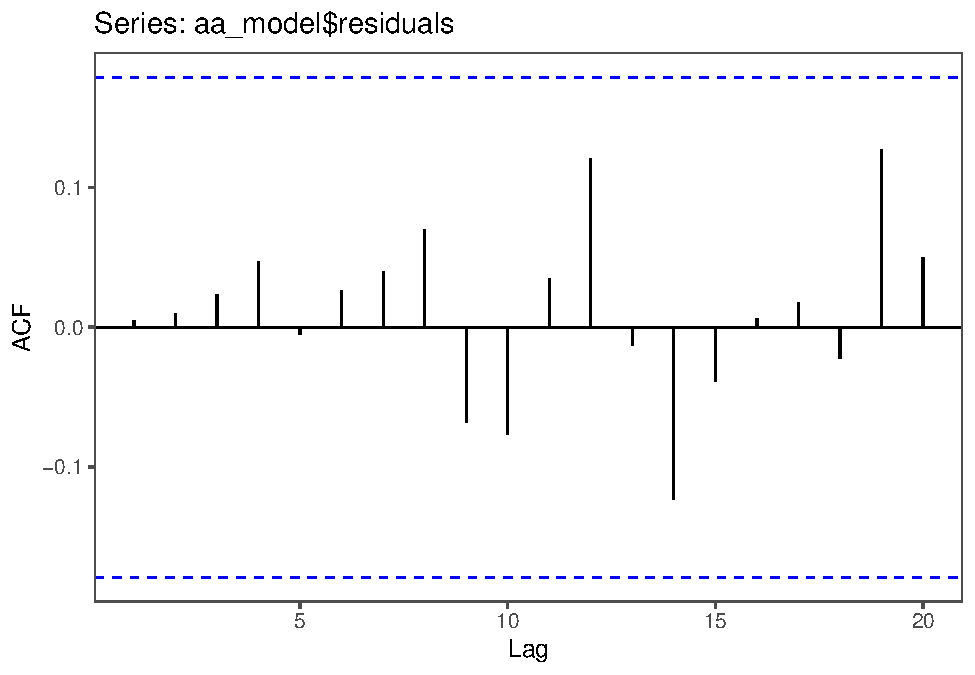
\includegraphics{Econo2_P3_files/figure-latex/estimation autoarima-1} \end{center}

\begin{Shaded}
	\begin{Highlighting}[]
		\KeywordTok{ggPacf}\NormalTok{(aa_model}\OperatorTok{$}\NormalTok{residuals, }\DataTypeTok{type =} \StringTok{"correlation"}\NormalTok{, }\DataTypeTok{lag.max =} \DecValTok{20}\NormalTok{, }
		\DataTypeTok{plot =}\NormalTok{ T) }\OperatorTok{+}\StringTok{ }\KeywordTok{theme_few}\NormalTok{()}
	\end{Highlighting}
\end{Shaded}

\begin{verbatim}
	## Warning: Ignoring unknown parameters: type
\end{verbatim}

\begin{center}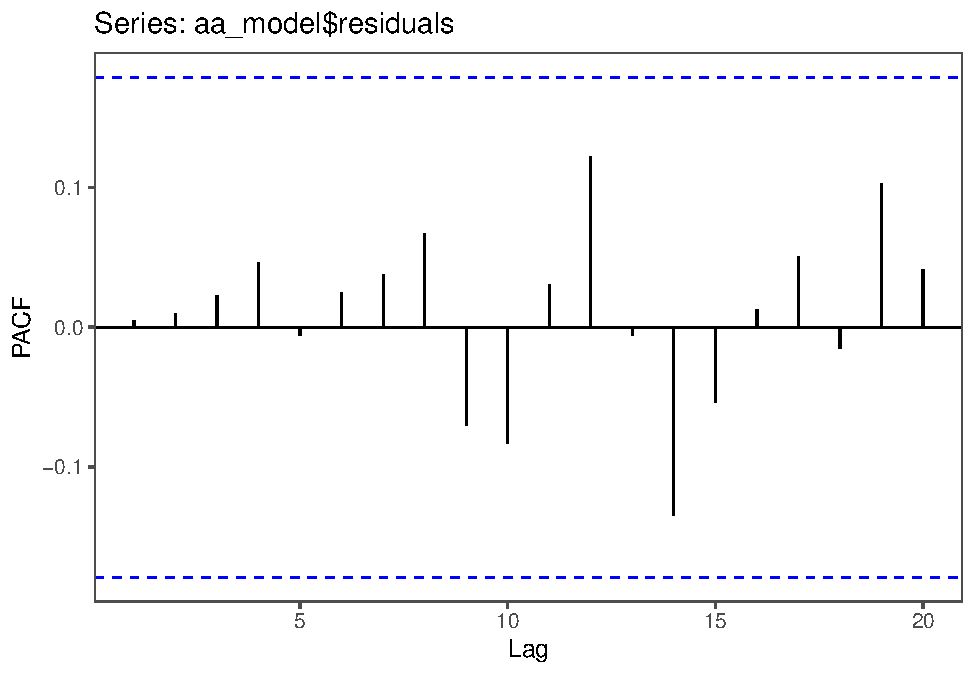
\includegraphics{Econo2_P3_files/figure-latex/estimation autoarima-2} \end{center}

The results of \emph{auto.arima} imply that the best model is an
ARMA(2,1):
\[ y_t = c + \Phi_1 y_{t-1} + \Phi_2 y_{t-2} + \theta_1 \varepsilon_{t-1} + \varepsilon_t, \hspace{1em} \varepsilon_t \sim wn(0, \sigma^2)\]

Furthermore, the Q-statistic \emph{(Box.test)} seems to indicate that
\(\varepsilon_t\) is truly white noise.

Let's now run some different models and compare them against the results
of \emph{auto.arima}. We'll begin with some overspecified model. First,
an ARMA(2,2):
\[ y_t = c + \Phi_1 y_{t-1} + \Phi_2 y_{t-2} + \theta_1 \varepsilon_{t-1} + \theta_2 \varepsilon_{t-2} + \varepsilon_t, \hspace{1em} \varepsilon_t \sim wn(0, \sigma^2)\]

\begin{Shaded}
	\begin{Highlighting}[]
		\NormalTok{arma22 <-}\StringTok{ }\KeywordTok{Arima}\NormalTok{(df}\OperatorTok{$}\NormalTok{value, }\DataTypeTok{order =} \KeywordTok{c}\NormalTok{(}\DecValTok{2}\NormalTok{, }\DecValTok{0}\NormalTok{, }\DecValTok{2}\NormalTok{))}
		
		\KeywordTok{summary}\NormalTok{(arma22)}
	\end{Highlighting}
\end{Shaded}

\begin{verbatim}
	## Series: df$value 
	## ARIMA(2,0,2) with non-zero mean 
	## 
	## Coefficients:
	##          ar1      ar2     ma1     ma2    mean
	##       0.7417  -0.5502  0.8113  0.0149  3.5311
	## s.e.  0.1442   0.0950  0.1692  0.1631  0.3514
	## 
	## sigma^2 estimated as 3.028:  log likelihood=-235.87
	## AIC=483.74   AICc=484.48   BIC=500.46
	## 
	## Training set error measures:
	##                      ME     RMSE      MAE      MPE     MAPE      MASE
	## Training set 0.01360342 1.703508 1.426237 4.791703 81.74486 0.5609619
	##                     ACF1
	## Training set 0.001161589
\end{verbatim}

\begin{Shaded}
	\begin{Highlighting}[]
		\NormalTok{arma22_t <-}\StringTok{ }\KeywordTok{matrix}\NormalTok{(}\OtherTok{NA}\NormalTok{, }\DataTypeTok{nrow =} \DecValTok{5}\NormalTok{)}
		
		\ControlFlowTok{for}\NormalTok{ (i }\ControlFlowTok{in} \KeywordTok{c}\NormalTok{(}\DecValTok{1}\OperatorTok{:}\DecValTok{5}\NormalTok{)) \{}
		
		\NormalTok{    arma22_t[i] <-}\StringTok{ }\NormalTok{arma22}\OperatorTok{$}\NormalTok{coef[i]}\OperatorTok{/}\KeywordTok{sqrt}\NormalTok{(arma22}\OperatorTok{$}\NormalTok{var.coef[i, i])}
		
		\NormalTok{\}}
		
		\NormalTok{arma22_t <-}\StringTok{ }\KeywordTok{data.frame}\NormalTok{(arma22_t)}
		
		\NormalTok{arma22_t}
	\end{Highlighting}
\end{Shaded}

\begin{verbatim}
	##      arma22_t
	## 1  5.14206433
	## 2 -5.78853038
	## 3  4.79577309
	## 4  0.09134106
	## 5 10.04968297
\end{verbatim}

\begin{Shaded}
	\begin{Highlighting}[]
		\NormalTok{arma22_q <-}\StringTok{ }\KeywordTok{Box.test}\NormalTok{(arma22}\OperatorTok{$}\NormalTok{residuals, }\DataTypeTok{lag =}\NormalTok{ arma22}\OperatorTok{$}\NormalTok{arma[}\DecValTok{1}\NormalTok{] }\OperatorTok{+}\StringTok{ }
		\StringTok{    }\NormalTok{arma22}\OperatorTok{$}\NormalTok{arma[}\DecValTok{2}\NormalTok{])}
		\NormalTok{arma22_q}
	\end{Highlighting}
\end{Shaded}

\begin{verbatim}
	## 
	##  Box-Pierce test
	## 
	## data:  arma22$residuals
	## X-squared = 0.26458, df = 4, p-value = 0.992
\end{verbatim}

The t-value of \(ma2\) is not able to reject the null hypothesis.
Furthermore, the Q-statistic \emph{(Box.test)} seems to indicate that
\(\varepsilon_t\) is truly white noise.

Now, an ARMA(3,1):
\[ y_t = c + \Phi_1 y_{t-1} + \Phi_2 y_{t-2} + \Phi_3 y_{t-3} + \theta_1 \varepsilon_{t-1} + \varepsilon_t, \hspace{1em} \varepsilon_t \sim wn(0, \sigma^2)\]

\begin{Shaded}
	\begin{Highlighting}[]
		\NormalTok{arma31 <-}\StringTok{ }\KeywordTok{Arima}\NormalTok{(df}\OperatorTok{$}\NormalTok{value, }\DataTypeTok{order =} \KeywordTok{c}\NormalTok{(}\DecValTok{3}\NormalTok{, }\DecValTok{0}\NormalTok{, }\DecValTok{1}\NormalTok{))}
		
		\KeywordTok{summary}\NormalTok{(arma31)}
	\end{Highlighting}
\end{Shaded}

\begin{verbatim}
	## Series: df$value 
	## ARIMA(3,0,1) with non-zero mean 
	## 
	## Coefficients:
	##          ar1     ar2     ar3     ma1    mean
	##       0.7610  -0.565  0.0112  0.7923  3.5312
	## s.e.  0.1215   0.137  0.1174  0.0825  0.3516
	## 
	## sigma^2 estimated as 3.028:  log likelihood=-235.87
	## AIC=483.74   AICc=484.48   BIC=500.46
	## 
	## Training set error measures:
	##                      ME     RMSE      MAE      MPE     MAPE      MASE
	## Training set 0.01359734 1.703504 1.426202 4.779284 81.71699 0.5609482
	##                      ACF1
	## Training set 0.0008885573
\end{verbatim}

\begin{Shaded}
	\begin{Highlighting}[]
		\NormalTok{arma31_t <-}\StringTok{ }\KeywordTok{matrix}\NormalTok{(}\OtherTok{NA}\NormalTok{, }\DataTypeTok{nrow =} \DecValTok{5}\NormalTok{)}
		
		\ControlFlowTok{for}\NormalTok{ (i }\ControlFlowTok{in} \KeywordTok{c}\NormalTok{(}\DecValTok{1}\OperatorTok{:}\DecValTok{5}\NormalTok{)) \{}
		
		\NormalTok{    arma31_t[i] <-}\StringTok{ }\NormalTok{arma31}\OperatorTok{$}\NormalTok{coef[i]}\OperatorTok{/}\KeywordTok{sqrt}\NormalTok{(arma31}\OperatorTok{$}\NormalTok{var.coef[i, i])}
		
		\NormalTok{\}}
		
		\NormalTok{arma31_t <-}\StringTok{ }\KeywordTok{data.frame}\NormalTok{(arma31_t)}
		
		\NormalTok{arma31_t}
	\end{Highlighting}
\end{Shaded}

\begin{verbatim}
	##      arma31_t
	## 1  6.26539086
	## 2 -4.12346904
	## 3  0.09501299
	## 4  9.59788435
	## 5 10.04172094
\end{verbatim}

\begin{Shaded}
	\begin{Highlighting}[]
		\NormalTok{arma31_q <-}\StringTok{ }\KeywordTok{Box.test}\NormalTok{(arma31}\OperatorTok{$}\NormalTok{residuals, }\DataTypeTok{lag =}\NormalTok{ arma31}\OperatorTok{$}\NormalTok{arma[}\DecValTok{1}\NormalTok{] }\OperatorTok{+}\StringTok{ }
		\StringTok{    }\NormalTok{arma31}\OperatorTok{$}\NormalTok{arma[}\DecValTok{2}\NormalTok{])}
		\NormalTok{arma31_q}
	\end{Highlighting}
\end{Shaded}

\begin{verbatim}
	## 
	##  Box-Pierce test
	## 
	## data:  arma31$residuals
	## X-squared = 0.25911, df = 4, p-value = 0.9923
\end{verbatim}

The t-value of \(ar3\) is not able to reject the null hypothesis.
Furthermore, the Q-statistic \emph{(Box.test)} seems to indicate that
\(\varepsilon_t\) is truly white noise.

Now, let's try some \emph{underspecified models}. Beginning with an
ARMA(2,0):
\[ y_t = c + \Phi_1 y_{t-1} + \Phi_2 y_{t-2} + \varepsilon_t, \hspace{1em} \varepsilon_t \sim wn(0, \sigma^2)\]

\begin{Shaded}
	\begin{Highlighting}[]
		\NormalTok{arma20 <-}\StringTok{ }\KeywordTok{Arima}\NormalTok{(df}\OperatorTok{$}\NormalTok{value, }\DataTypeTok{order =} \KeywordTok{c}\NormalTok{(}\DecValTok{2}\NormalTok{, }\DecValTok{0}\NormalTok{, }\DecValTok{0}\NormalTok{))}
		
		\KeywordTok{summary}\NormalTok{(arma20)}
	\end{Highlighting}
\end{Shaded}

\begin{verbatim}
	## Series: df$value 
	## ARIMA(2,0,0) with non-zero mean 
	## 
	## Coefficients:
	##          ar1      ar2    mean
	##       1.0226  -0.7153  3.5194
	## s.e.  0.0634   0.0635  0.2694
	## 
	## sigma^2 estimated as 4.24:  log likelihood=-256.37
	## AIC=520.74   AICc=521.09   BIC=531.89
	## 
	## Training set error measures:
	##                      ME     RMSE      MAE      MPE     MAPE      MASE      ACF1
	## Training set 0.01106086 2.033314 1.630805 73.16585 128.4039 0.6414218 0.2915253
\end{verbatim}

\begin{Shaded}
	\begin{Highlighting}[]
		\NormalTok{arma20_t <-}\StringTok{ }\KeywordTok{matrix}\NormalTok{(}\OtherTok{NA}\NormalTok{, }\DataTypeTok{nrow =} \DecValTok{3}\NormalTok{)}
		
		\ControlFlowTok{for}\NormalTok{ (i }\ControlFlowTok{in} \KeywordTok{c}\NormalTok{(}\DecValTok{1}\OperatorTok{:}\DecValTok{3}\NormalTok{)) \{}
		
		\NormalTok{    arma20_t[i] <-}\StringTok{ }\NormalTok{arma20}\OperatorTok{$}\NormalTok{coef[i]}\OperatorTok{/}\KeywordTok{sqrt}\NormalTok{(arma20}\OperatorTok{$}\NormalTok{var.coef[i, i])}
		
		\NormalTok{\}}
		
		\NormalTok{arma20_t <-}\StringTok{ }\KeywordTok{data.frame}\NormalTok{(arma20_t)}
		
		\NormalTok{arma20_t}
	\end{Highlighting}
\end{Shaded}

\begin{verbatim}
	##    arma20_t
	## 1  16.12226
	## 2 -11.26848
	## 3  13.06561
\end{verbatim}

\begin{Shaded}
	\begin{Highlighting}[]
		\NormalTok{arma20_q <-}\StringTok{ }\KeywordTok{Box.test}\NormalTok{(arma20}\OperatorTok{$}\NormalTok{residuals, }\DataTypeTok{lag =}\NormalTok{ arma20}\OperatorTok{$}\NormalTok{arma[}\DecValTok{1}\NormalTok{] }\OperatorTok{+}\StringTok{ }
		\StringTok{    }\NormalTok{arma20}\OperatorTok{$}\NormalTok{arma[}\DecValTok{2}\NormalTok{])}
		\NormalTok{arma20_q}
	\end{Highlighting}
\end{Shaded}

\begin{verbatim}
	## 
	##  Box-Pierce test
	## 
	## data:  arma20$residuals
	## X-squared = 13.728, df = 2, p-value = 0.001045
\end{verbatim}

The Q-statistic indicates that there is an ommited variable -- namely,
\(\varepsilon_{t-1}\) that we have just excluded from the model.

Now, an ARMA(1,1):
\[ y_t = c + \Phi_1 y_{t-1} +  + \theta_1 \varepsilon_{t-1} + \varepsilon_t, \hspace{1em} \varepsilon_t \sim wn(0, \sigma^2)\]

\begin{Shaded}
	\begin{Highlighting}[]
		\NormalTok{arma11 <-}\StringTok{ }\KeywordTok{Arima}\NormalTok{(df}\OperatorTok{$}\NormalTok{value, }\DataTypeTok{order =} \KeywordTok{c}\NormalTok{(}\DecValTok{1}\NormalTok{, }\DecValTok{0}\NormalTok{, }\DecValTok{1}\NormalTok{))}
		
		\KeywordTok{summary}\NormalTok{(arma11)}
	\end{Highlighting}
\end{Shaded}

\begin{verbatim}
	## Series: df$value 
	## ARIMA(1,0,1) with non-zero mean 
	## 
	## Coefficients:
	##          ar1     ma1    mean
	##       0.4476  0.9244  3.6027
	## s.e.  0.0831  0.0323  0.6234
	## 
	## sigma^2 estimated as 4.026:  log likelihood=-253.74
	## AIC=515.48   AICc=515.82   BIC=526.63
	## 
	## Training set error measures:
	##                       ME     RMSE      MAE      MPE     MAPE      MASE
	## Training set 0.006283661 1.981184 1.621537 51.07775 142.3988 0.6377767
	##                   ACF1
	## Training set 0.2028683
\end{verbatim}

\begin{Shaded}
	\begin{Highlighting}[]
		\NormalTok{arma11_t <-}\StringTok{ }\KeywordTok{matrix}\NormalTok{(}\OtherTok{NA}\NormalTok{, }\DataTypeTok{nrow =} \DecValTok{3}\NormalTok{)}
		
		\ControlFlowTok{for}\NormalTok{ (i }\ControlFlowTok{in} \KeywordTok{c}\NormalTok{(}\DecValTok{1}\OperatorTok{:}\DecValTok{3}\NormalTok{)) \{}
		
		\NormalTok{    arma11_t[i] <-}\StringTok{ }\NormalTok{arma11}\OperatorTok{$}\NormalTok{coef[i]}\OperatorTok{/}\KeywordTok{sqrt}\NormalTok{(arma11}\OperatorTok{$}\NormalTok{var.coef[i, i])}
		
		\NormalTok{\}}
		
		\NormalTok{arma11_t <-}\StringTok{ }\KeywordTok{data.frame}\NormalTok{(arma11_t)}
		
		\NormalTok{arma11_t}
	\end{Highlighting}
\end{Shaded}

\begin{verbatim}
	##    arma11_t
	## 1  5.387948
	## 2 28.624391
	## 3  5.779126
\end{verbatim}

\begin{Shaded}
	\begin{Highlighting}[]
		\NormalTok{arma11_q <-}\StringTok{ }\KeywordTok{Box.test}\NormalTok{(arma11}\OperatorTok{$}\NormalTok{residuals, }\DataTypeTok{lag =}\NormalTok{ arma11}\OperatorTok{$}\NormalTok{arma[}\DecValTok{1}\NormalTok{] }\OperatorTok{+}\StringTok{ }
		\StringTok{    }\NormalTok{arma11}\OperatorTok{$}\NormalTok{arma[}\DecValTok{2}\NormalTok{])}
		\NormalTok{arma11_q}
	\end{Highlighting}
\end{Shaded}

\begin{verbatim}
	## 
	##  Box-Pierce test
	## 
	## data:  arma11$residuals
	## X-squared = 12.668, df = 2, p-value = 0.001775
\end{verbatim}

Again, the Q-statistic indicates that there is an ommited variable --
namely, \(y_{t-1}\) that we have just excluded from the model.

Finally, let's compare the \(AIC\) and \(BIC\) values for all these
models.

\begin{Shaded}
	\begin{Highlighting}[]
		\NormalTok{criteria <-}\StringTok{ }\KeywordTok{matrix}\NormalTok{(}\OtherTok{NA}\NormalTok{, }\DataTypeTok{nrow =} \DecValTok{5}\NormalTok{, }\DataTypeTok{ncol =} \DecValTok{3}\NormalTok{)}
		
		\NormalTok{aa_criteria <-}\StringTok{ }\KeywordTok{data.frame}\NormalTok{(}\StringTok{"ARMA(2,1)*"}\NormalTok{, aa_model}\OperatorTok{$}\NormalTok{aic, aa_model}\OperatorTok{$}\NormalTok{bic)}
		
		\KeywordTok{names}\NormalTok{(aa_criteria) <-}\StringTok{ }\KeywordTok{c}\NormalTok{(}\StringTok{"Model"}\NormalTok{, }\StringTok{"AIC"}\NormalTok{, }\StringTok{"BIC"}\NormalTok{)}
		
		\NormalTok{arma22_criteria <-}\StringTok{ }\KeywordTok{data.frame}\NormalTok{(}\StringTok{"ARMA(2,2)"}\NormalTok{, arma22}\OperatorTok{$}\NormalTok{aic, arma22}\OperatorTok{$}\NormalTok{bic)}
		
		\KeywordTok{names}\NormalTok{(arma22_criteria) <-}\StringTok{ }\KeywordTok{c}\NormalTok{(}\StringTok{"Model"}\NormalTok{, }\StringTok{"AIC"}\NormalTok{, }\StringTok{"BIC"}\NormalTok{)}
		
		\NormalTok{arma31_criteria <-}\StringTok{ }\KeywordTok{data.frame}\NormalTok{(}\StringTok{"ARMA(3,1)"}\NormalTok{, arma31}\OperatorTok{$}\NormalTok{aic, arma31}\OperatorTok{$}\NormalTok{bic)}
		
		\KeywordTok{names}\NormalTok{(arma31_criteria) <-}\StringTok{ }\KeywordTok{c}\NormalTok{(}\StringTok{"Model"}\NormalTok{, }\StringTok{"AIC"}\NormalTok{, }\StringTok{"BIC"}\NormalTok{)}
		
		\NormalTok{arma20_criteria <-}\StringTok{ }\KeywordTok{data.frame}\NormalTok{(}\StringTok{"ARMA(2,0)"}\NormalTok{, arma20}\OperatorTok{$}\NormalTok{aic, arma20}\OperatorTok{$}\NormalTok{bic)}
		
		\KeywordTok{names}\NormalTok{(arma20_criteria) <-}\StringTok{ }\KeywordTok{c}\NormalTok{(}\StringTok{"Model"}\NormalTok{, }\StringTok{"AIC"}\NormalTok{, }\StringTok{"BIC"}\NormalTok{)}
		
		\NormalTok{arma11_criteria <-}\StringTok{ }\KeywordTok{data.frame}\NormalTok{(}\StringTok{"ARMA(1,1)"}\NormalTok{, arma11}\OperatorTok{$}\NormalTok{aic, arma11}\OperatorTok{$}\NormalTok{bic)}
		
		\KeywordTok{names}\NormalTok{(arma11_criteria) <-}\StringTok{ }\KeywordTok{c}\NormalTok{(}\StringTok{"Model"}\NormalTok{, }\StringTok{"AIC"}\NormalTok{, }\StringTok{"BIC"}\NormalTok{)}
		
		
		\NormalTok{criteria <-}\StringTok{ }\KeywordTok{rbind.data.frame}\NormalTok{(aa_criteria, arma22_criteria, arma31_criteria, }
		\NormalTok{    arma20_criteria, arma11_criteria)}
		
		\NormalTok{criteria}
	\end{Highlighting}
\end{Shaded}

\begin{verbatim}
	##        Model      AIC      BIC
	## 1 ARMA(2,1)* 481.7460 495.6834
	## 2  ARMA(2,2) 483.7376 500.4625
	## 3  ARMA(3,1) 483.7369 500.4619
	## 4  ARMA(2,0) 520.7381 531.8880
	## 5  ARMA(1,1) 515.4753 526.6253
\end{verbatim}

As we can clearly see, the model chosen by \emph{auto.arima} is the
optimal choice according both to AIC and BIC.




\chapter{Forecasting}

Suppose that you observe a time series up to period T, $Y_1, Y_2, ..., Y_T,$ and would like to forecast its value in $T+1$, or, more generically, up to a time horizon $h \geq 1$: $Y_{T+1}, ..., Y_{T+h}$.

Let $g(Y_1, ..., Y_T)$ be a general predictor of $Y_{T+1}$ built with information up to period $T$. We can measure its utility with its \textit{mean squared error (MSE)}:
$$ MSE[g(Y_1, ..., Y_T)] := \mathbb{E}[(Y_{T+1} - g(Y_1, ..., Y_T))^2] $$

We know that the conditional mean is the predictor that minimizes MSE:
$$\mathbb{E}\left(Y_{T+1} \mid Y_{T}, \ldots, Y_{1}\right)=\operatorname{argmin}_{g} \mathbb{E}\left[\left(Y_{t+1}-g\left(Y_{1}, Y_{2}, \ldots, Y_{T}\right)\right)^{2}\right]$$

Unfortunately, we usually don't have the functional form of $\mathbb{E}\left(Y_{T+1} \mid Y_{T}, \ldots, Y_{1}\right)$, and postulate its best linear form:
$$\pi\left(Y_{T+1} \mid Y_{T}, \ldots, Y_{1}\right)=\alpha+\beta_{0} Y_{T}+\beta_{1} Y_{T-1}+\ldots \beta_{T-1} Y_{1}$$

Denote the best linear predictor with information up to T as $Y_{T+1|T} := \pi(Y_{T+1}|Y_t,..., Y_1)$, and its estimated version as $\hat{Y}_{T+1|T} := \hat{\pi}(Y_{T+1}|Y_t,..., Y_1) = \hat{\alpha}+\hat{\beta}_{0} Y_{T}+\hat{\beta}_{1} Y_{T-1}+\ldots \hat{\beta}_{T-1} Y_{1}$.

\section{Forecasting with an AR(1) model}

Remember from Definition \ref{ar1-def} that an AR(1) model has the following form:
$$ Y_t = c + \phi Y_{t-1} + \varepsilon_{t}$$

\subsection{Forecast}

Given that $\mathbb{E}(\varepsilon_{t+1}|Y_T) = 0$ (as $\varepsilon \sim wn(0, \sigma^2)$), we have: 

$$
Y_{T+1 \mid T}:=\pi\left(Y_{T+1} \mid Y_{T}, \ldots, Y_{1}\right)=c+\phi Y_{T}
$$
For $T+2$, we have:
$$
\begin{aligned}
	Y_{T+2 \mid T} &:=\pi\left(Y_{T+2} \mid Y_{T}, \ldots, Y_{1}\right) \\
	&=\pi\left(\pi\left(Y_{T+2} \mid Y_{T+1}, Y_{T}, \ldots, Y_{1}\right) \mid Y_{T}, \ldots, Y_{1}\right) \\
	&=\pi\left(c+\phi Y_{T+1} \mid Y_{T}, \ldots, Y_{1}\right) \\
	&=c+\phi\left(c+\phi Y_{T}\right)=(1+\phi) c+\phi^{2} Y_{T}
\end{aligned}
$$
The clear pattern here yields, more generally:
$$
Y_{T+h \mid T}=\left(1+\phi+\phi^{2}+\cdots+\phi^{h-1}\right) c+\phi^{h} Y_{T}
$$

\subsection{Forecast error}

It is also easy to verify that the \textit{forecast error} for $h=1$ is given by:
$$ u_{T+1|T} := Y_{T+1} - Y_{T+1|T} = Y_{T+1} - c - \phi Y_T = \varepsilon_{T+1} $$
 
For $h=2$, we have:
$$
\begin{aligned}
 u_{T+2 \mid T} &:=Y_{T+2}-Y_{T+2 \mid T} \\
 &=c+\phi Y_{T+1}+\varepsilon_{T+2}-\left(c+\phi Y_{T+1 \mid T}\right) \\
 &=\phi\left(Y_{T+1}-Y_{T+1 \mid T}\right)+\varepsilon_{T+2} \\
 &=\phi u_{T+1 \mid T}+\varepsilon_{T+2}=\phi \varepsilon_{T+1}+\varepsilon_{T+2}
\end{aligned}
$$
More generally, for a given time horizon $h$:
$$
u_{T+h \mid T}=\left(\varepsilon_{T+h}+\phi \varepsilon_{T+h-1}+\cdots+\phi^{h-1} \varepsilon_{T+1}\right)$$

\subsection{Mean reversion}

Note that, as $h$ increases, the prediction \textit{reverts to the unconditional mean:}

$$\lim _{h \rightarrow \infty} Y_{T+h \mid T}=c \lim _{h \rightarrow \infty} \sum_{i=0}^{h-1} \phi^{i}+Y_{T} \lim _{h \rightarrow \infty} \phi^{h}=\frac{c}{1-\phi}=: \mu$$

The variance of the forecast error is given by:
$$ Var(u_{T+h|T}) = (1 + \phi^{2} + \phi^4 + ... + \phi^{2(h-1)})\sigma^2 $$

Taking the limit as $h \to \infty$, the variance of the forecast error \textit{also approaches the unconditional variance of the process:}
$$\lim _{h \rightarrow \infty} \mathbb{V}\left(u_{T+h \mid T}\right)=\sigma^{2} \lim _{h \rightarrow \infty} \sum_{i=0}^{h-1} \phi^{2 i}=\frac{\sigma^{2}}{1-\phi^{2}}=: \gamma_{0}$$

\section{Forecasting with an AR(p) model}

\subsection{Forecast}

The same procedure can be applied to an AR(p). For $h = 1$: 
$$
Y_{T+1 \mid T}=\pi\left(Y_{T+1} \mid Y_{T}, \ldots, Y_{1}\right)=c+\phi_{1} Y_{T}+\cdots+\phi_{p} Y_{T-p+1}
$$
For a given $h$, proceed recursively:
$$\begin{aligned}
	Y_{T+2 \mid T} &=c+\phi_{1} Y_{T+1 \mid T}+\phi_{2} Y_{T}+\phi_{3} Y_{T-1}+\cdots+\phi_{p} Y_{T+2-p} \\
	Y_{T+3 \mid T} &=c+\phi_{1} Y_{T+2 \mid T}+\phi_{2} Y_{T+1 \mid T}+\phi_{3} Y_{T}+\cdots+\phi_{p} Y_{T+3-p} \\
	Y_{T+4 \mid T} &=c+\phi_{1} Y_{T+3 \mid T}+\phi_{2} Y_{T+2 \mid T}+\phi_{3} Y_{T+1 \mid T}+\cdots+\phi_{p} Y_{T+4-p} \\
	& \vdots \\
	Y_{T+h \mid T} &=c+\phi_{1} Y_{T+h-1 \mid T}+\phi_{2} Y_{T+h-2 \mid T}+\cdots+\phi_{p} Y_{T+h-p \mid T}
\end{aligned}$$

\subsection{Forecast error}

For $h=1$, the forecast error is given by:
$$ u_{T+1|T} := Y_{T+1} - Y_{T+1|T} = \varepsilon_{T+1}$$

As $h$ increases:
$$\begin{aligned}
	u_{T+2 \mid T} &=\phi_{1} u_{T+1 \mid T}+\varepsilon_{T+2} \\
	u_{T+3 \mid T} &=\phi_{1} u_{T+2 \mid T}+\phi_{2} u_{T+1 \mid T}+\varepsilon_{T+3} \\
	& \vdots \\
	u_{T+h \mid T} &=\phi_{1} u_{T+h-1 \mid T}+\cdots+\phi_{h-1} u_{T+1 \mid T}+\varepsilon_{T+h},
\end{aligned}$$
where $\phi_{h-1} = 0$ for $h-1>p$.

\section{Forecasting with a MA(1) model}

Remember from \ref{ma1-def} that a MA(1) model is given by
$$ Y_t = c + \theta \varepsilon_{t-1} + \varepsilon_{t} $$
$$ Y_{T+1|T} := \pi(Y_{T+1} | Y_T,..., Y_1) $$

We have seen that, if the MA(1) is invertible, we can write it as an AR($\infty$). This would mean, however, that the forecast errors would depend on \textit{all past values} -- notwithstanding the decreasing dependence, due to ergodicity. Given a fixed $\varepsilon_{0}$, we can reconstruct the entire error series: 
$$\begin{aligned}
	\varepsilon_{1} &=Y_{1}-c-\theta \varepsilon_{0} \\
	\varepsilon_{2} &=Y_{2}-c-\theta \varepsilon_{1} \\
	& \vdots \\
	\varepsilon_{T} &=Y_{T}-c-\theta \varepsilon_{T-1}
\end{aligned}$$

If we do not know $\varepsilon_{0}$, we can approximate it by its (known!) mean, $\tilde{\varepsilon}_0 = 0$. If $T$ is large enough and $|\theta| < 1$, this is a good approximation. That is the case because for large $T$, the influence of the assumption $\tilde{\varepsilon}_0 = 0$ is geometrically diminished over time, given $|\theta| < 1$. 


\subsection{Forecast}

We are now able to construct the forecast using the estimated $\tilde{\varepsilon}_T$.
$$ Y_{T+1|T} := c + \theta \tilde{\varepsilon}_T $$

Iteratively for larger horizons:
$$Y_{T+2 \mid T}=c+\theta \widetilde{\varepsilon}_{T+1}=c+\theta\left(Y_{T+1 \mid T}-c-\theta \widetilde{\varepsilon}_{T}\right)=c$$

Note that \textit{the MA(1) process is not predictable for $h > 1$.} The forecast immediately mean reverts at $h>1$.

\subsection{Forecast error}

The forecast error, assuming $\tilde{\varepsilon}_T \approx \varepsilon_{T}$, is given by: 
$$ u_{T+1|T} := Y_{T+1} - Y_{T+1|T} = \varepsilon_{T+1}$$

This means that the variance of the forecast error is $\sigma^2$. For larger horizons, the variance converges to the unconditional variance: 
$$ u_{T+h|T} := Y_{T+h} - Y_{T+h|T} = \varepsilon_{T+h} + \theta \varepsilon_{T+h-1}, \forall h>1$$

Thus, $ Var(u_{T+h|T}) = (1+\theta)^2 \sigma^2 = \gamma_0, \forall h > 1$.

\section{Forecasting with a MA(q) model}

We can proceed iteratively for the MA(q) model.

$$\begin{aligned}
	Y_{T+1 \mid T} &=c+\theta_{1} \widetilde{\varepsilon}_{T}+\cdots+\theta_{q} \widetilde{\varepsilon}_{T+1-q} \\
	Y_{T+2 \mid T} &=c+\theta_{2} \widetilde{\varepsilon}_{T}+\cdots+\theta_{q} \widetilde{\varepsilon}_{T+2-q} \\
	Y_{T+3 \mid T} &=c+\theta_{3} \widetilde{\varepsilon}_{T}+\cdots+\theta_{q} \widetilde{\varepsilon}_{T+3-q} \\
	& \vdots \\
	Y_{T+q \mid T} &=c+\theta_{q} \widetilde{\varepsilon}_{T}
\end{aligned}$$

Note that, after $q$ periods, the prediction is the unconditional mean $c$.

\section{Forecast with an ARMA(p,q) model}

Let's combine the procedures presented for AR(p) and MA(q). For $h=1$:
$$Y_{T+1 \mid T}=c+\phi_{1} Y_{T}+\cdots+\phi_{p} Y_{T-p+1}+\theta_{1} \widetilde{\varepsilon}_{T}+\cdots+\theta_{q} \widetilde{\varepsilon}_{T+1-q},$$
where $\{\widetilde{\varepsilon}_{T}, ..., \widetilde{\varepsilon}_{T+1-q}\}$ were obtained from the reconstruction process explained in the MA(q) case. However, here we need, aside from the first $q$ innovation values, also the \textit{last $p$ observations before the first one}. That is the case because of the expression for $\widetilde{\varepsilon}_{1}$:

$$\widetilde{\varepsilon}_{1}=Y_{1}-c-\phi_{1} Y_{0}-\cdots-\phi_{p} Y_{p-1}-\theta_{1} \widetilde{\varepsilon}_{0}-\theta_{2} \widetilde{\varepsilon}_{-1}-\cdots-\theta_{q} \widetilde{\varepsilon}_{1-q}$$

Alternatively, we can start reconstructing the residuals from $p+1$. 

\subsection{Forecast}

From this, we can obtain the forecasts for any horizon $h \geq 1$, given $h>p>q$: 
$$\begin{array}{l}
	Y_{T+1 \mid T}=c+\phi_{1} Y_{T}+\cdots+\phi_{p} Y_{T+1-p}+\theta_{1} \widetilde{\varepsilon}_{T}+\cdots+\theta_{q} \widetilde{\varepsilon}_{T+1-q} \\
	Y_{T+2 \mid T}=c+\phi_{1} Y_{T+1 \mid T}+\cdots+\phi_{p} Y_{T+2-p}+\theta_{2} \widetilde{\varepsilon}_{T}+\cdots+\theta_{q} \widetilde{\varepsilon}_{T+2-q} \\
	Y_{T+3 \mid T}=c+\phi_{1} Y_{T+2 \mid T}+\cdots+\phi_{p} Y_{T+3-p}+\theta_{3} \widetilde{\varepsilon}_{T}+\cdots+\theta_{q} \widetilde{\varepsilon}_{T+3-q}
\end{array}$$

$ \hspace{13em} \vdots$

$$\begin{aligned}
	Y_{T+q \mid T} &=c+\phi_{1} Y_{T+q-1 \mid T}+\cdots+\phi_{p} Y_{T+q-p}+\theta_{q} \widetilde{\varepsilon}_{T} \\
	Y_{T+q+1 \mid T} &=c+\phi_{1} Y_{T+q \mid T}+\cdots+\phi_{p} Y_{T+q+1-p} \\
	& \vdots \\
	Y_{T+h \mid T} &=c+\phi_{1} Y_{T+h-1 \mid T}+\cdots+\phi_{p} Y_{T+h-p \mid T}
\end{aligned}$$

\section{Confidence intervals for forecasts}

Given a forecast $\hat{Y}_{T+h|T}$, we'd like to have a \textit{confidence interval} for it. In practice, forecasting involves two types of errors:
\begin{itemize}
	\item \textbf{Estimation error:} $Y_{T+h|T} - \hat{Y}_{T+h|T}$. This is due to the estimation of the ARMA model, as we are always working with a sample.
	\item \textbf{Forecast error:} $u_{T+h|T} = Y_{T+h} - Y_{T+h|T}$. This is the portion of the error that would exist event if we knew the true population parameters.
\end{itemize}

From this, we have the \textit{aggregate error:}
$$ Y_{T+h} - \hat{Y}_{T+h|T} = (Y_{T+h} - {Y}_{T+h|T}) + (Y_{T+h|T} - \hat{Y}_{T+h|T}) $$

\subsection{Normally distributed errors}

A first way to tackle the issue of confidence intervals for forecasts is to \textit{assume normality}: $\varepsilon_{t} \sim \mathcal{N}(0, \sigma^2)$. 

In that case, we know that $Y_{T+h}, \hat{Y}_{T+h|T}$ will also be normally distributed, as the first term consists of a combination of past errors and past values of Y, and the second term is asymptotically normal given the properties of ARMA estimators. This means that the confidence interval is known to us, for $\alpha = 5\%$:
$$\left[\widehat{Y}_{T+h \mid T} \pm 1,96 \sqrt{\mathbb{V}\left(u_{T+h \mid T}\right)}\right]$$

We clearly do not observe $Var(u_{T+h|T})$, but we know its functional form and, thus, can consistently estimate it. For an AR(1), for example: 
$$\widehat{\mathbb{V}}\left(u_{T+h \mid T}\right)=\widehat{\sigma}^{2} \sum_{i=0}^{h-1} \widehat{\phi}^{2 i}$$

Note that, even if we assume that the innovation terms are normally distributed, we \textit{still need an asymptotic argument} to guarantee that $\widehat{Y}_{T+h \mid T} \stackrel{p}{\longrightarrow} Y_{T+h \mid T} \text { and } \widehat{\mathbb{V}}\left(u_{T+h \mid T}\right) \stackrel{p}{\longrightarrow} \mathbb{V}\left(u_{T+h \mid T}\right)$.

\subsection{Bootstrapping}

What if the errors \textit{are not normally distributed?} This makes the issue a lot more complicated. Note that, even if we apply the CLT to argue that $Y_{T+h|T} - \hat{Y}_{T+h|T} \sim \mathcal{N}(\cdot)$, what makes us believe that $(Y_{T+h} - {Y}_{T+h|T})$ is also normally distributed? In the last subsection, this condition was valid because of the distribution of the errors. There's no asymptotical argument to be made. 

In practice, we don't know the distribution of the error terms. In fact, they are \textit{rarely normally distributed!} A procedure to construct confidence intervals in this setting is called \textit{bootstrap.} For ARMA models, it consists in generating simulated samples from the actual sample and repeat the estimations for each simulated sample. This yields an arbitrarily large number of estimates \textit{from the same data}. From this, we can use its \textit{empirical distribution} to find the confidence interval.

Bootstrapping has a number of advantages over the traditional procedures for obtaining a confidence interval. In many cases, the convergence is faster than the usual $1/\sqrt{T}$, and it frequently performs better in small sample environments. It can also be applied in settings in which asymptotic theory is very intricate. In practice, we almost always use some sort of bootstrap method. 

The essential idea behind bootstrapping is to assume that $\varepsilon_{t}$ is \textit{iid} with a cdf $F$. Suppose that you have $T$ residuals, $\hat{\varepsilon}_t$. Its empirical distribution is simply: 
$$ \hat{F}_T(v) = \dfrac{\{ no. \, residuals \leq v \}}{T}, \hspace{1em} v \in \mathbb{R}$$

The Law of Large Numbers guarantees that, as $T \to \infty$, 
$$ \hat{F}_T(v) \to_{a.s.} F(v) $$
This means that the empirical distribution of the residuals becomes arbitrarily close to the real distribution as $T$ grows.

\subsubsection{Procedure}

Bootstrapping for an ARMA(p,q) model involves the following steps:

\begin{enumerate}
	\item \begin{itemize}
		\item Estimate ARMA(p,q)
		$$ Y_t = c + \sum_{j=1}^p \phi_j Y_{t-j} + \sum_{j=1}^q \theta_j \varepsilon_{t-j} + \varepsilon_t$$
		
		\item Calculate the residuals of the regression:
		$$ \hat{\varepsilon}_t := Y_t - (\hat{c} + \sum_{j=1}^p \hat{\phi}_j Y_{t-j} + \sum_{j=1}^q \hat{\theta}_j \varepsilon_{t-j})$$
		
		\item If the residuals do not have mean 0, create the centered residuals:
		$$ \tilde{\varepsilon}_t = \hat{\varepsilon}_t - \frac{1}{t} \sum_{t=1}^T \hat{\varepsilon}_t$$
	\end{itemize}
	
	\item \begin{itemize}
		\item Select at random, with replacement, a sample with $T + m$ elements, $m >> 0$:
		$$\{\varepsilon^*_1, ..., \varepsilon^*_{T+m}\}$$
		\item Create a series $\{Y^*_t\}_{t=1}^{T+m}$:
		$$ Y_t^* = Y_t, 1 \leq t \leq max(p,q) $$
		$$ Y_t^* = \hat{c} + \sum_{j=1}^p \hat{\phi}_j Y_{t-j} + \sum_{j=1}^q \hat{\theta}_j \varepsilon_{t-j}^* + \varepsilon_t^*, max(p,q) < t \leq T + m $$
	\end{itemize}
	\item \begin{itemize}
		\item Using the simulated sample $\{Y^*_t\}_{t=1}^{T+m}$, create a forecast for $h >0$ periods using the estimated coefficients \textit{obtained with the real sample}.
		\item This yields a vector of dimension $h$ containing the forecasts in the form:
		$$(\hat{Y}^*_{T+1}, ..., \hat{Y}^*_{T+h})$$ 
		\item Repeat steps 2 and 3 for $S$ times. Create a matrix with the results.
		\item This yields a S x h matrix where each row is equal to the aforementioned vector.
	\end{itemize}
\end{enumerate}

\chapter{Problem 4: Cross-validation and bootstrap}

In this problem, we'll be tackling the issue of \emph{forecasting} of an
ARMA model. The problem is split in two parts: (i)
\emph{cross-validation}; and (ii) \emph{bootstrapping}.

\section{Identification and estimation}

First, let's identify the best model for our time series.

\begin{Shaded}
	\begin{Highlighting}[]
		\NormalTok{df <-}\StringTok{ }\KeywordTok{data.frame}\NormalTok{(df)}
		
		\NormalTok{pplot <-}\StringTok{ }\KeywordTok{ggplot}\NormalTok{(}\DataTypeTok{data =}\NormalTok{ df, }\KeywordTok{aes}\NormalTok{(}\DataTypeTok{x =}\NormalTok{ t, }\DataTypeTok{y =}\NormalTok{ value)) }\OperatorTok{+}\StringTok{ }\KeywordTok{geom_line}\NormalTok{() }\OperatorTok{+}\StringTok{ }
		\StringTok{    }\KeywordTok{ggtitle}\NormalTok{(}\StringTok{"Time series plot"}\NormalTok{) }\OperatorTok{+}\StringTok{ }\KeywordTok{theme_few}\NormalTok{()}
		\NormalTok{pplot}
	\end{Highlighting}
\end{Shaded}

\begin{center}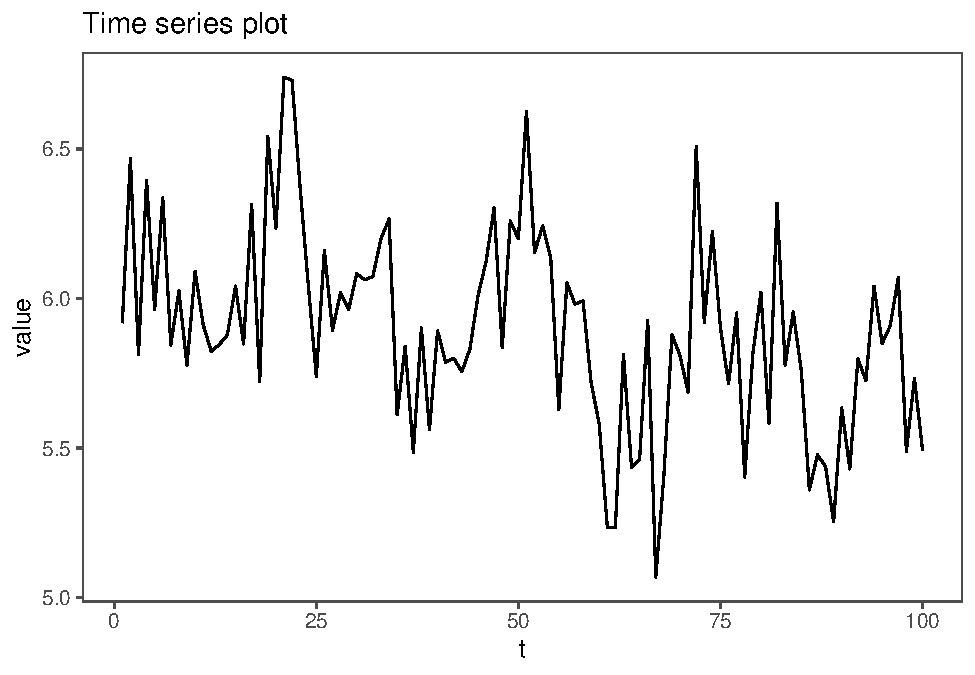
\includegraphics{Econo2_P4_files/figure-latex/plots-1} \end{center}

\begin{Shaded}
	\begin{Highlighting}[]
		\NormalTok{acf_ts <-}\StringTok{ }\KeywordTok{Acf}\NormalTok{(df}\OperatorTok{$}\NormalTok{value, }\DataTypeTok{lag.max =} \DecValTok{5000}\NormalTok{)}
	\end{Highlighting}
\end{Shaded}

\begin{center}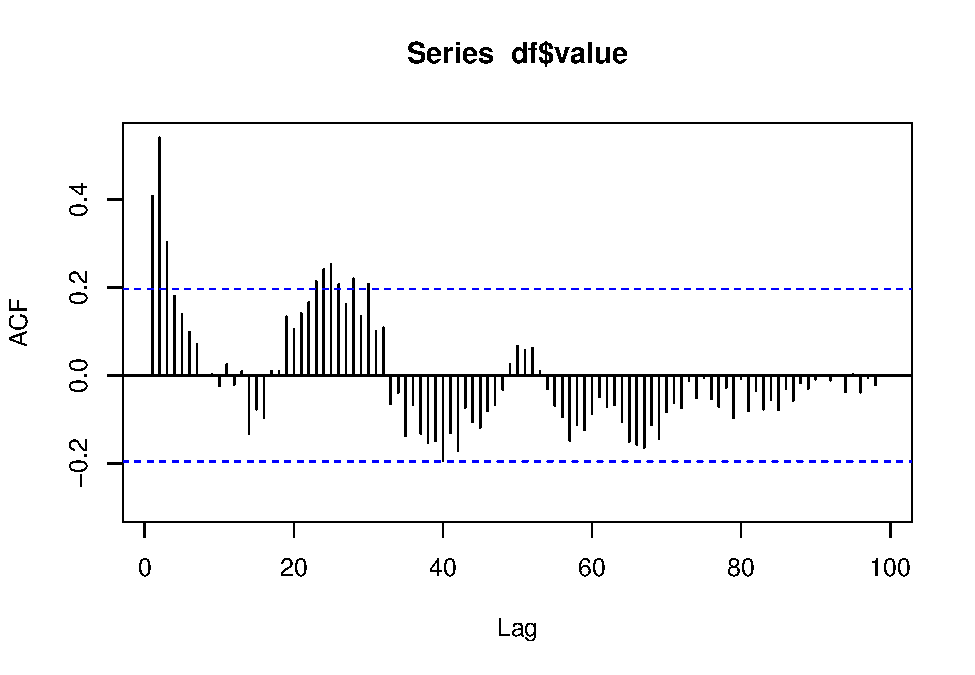
\includegraphics{Econo2_P4_files/figure-latex/plots-2} \end{center}

\begin{Shaded}
	\begin{Highlighting}[]
		\NormalTok{acf_test_values <-}\StringTok{ }\NormalTok{acf_ts}\OperatorTok{$}\NormalTok{acf}\OperatorTok{/}\KeywordTok{sd}\NormalTok{(acf_ts}\OperatorTok{$}\NormalTok{acf)}
		
		\KeywordTok{head}\NormalTok{(}\KeywordTok{data.frame}\NormalTok{(acf_test_values))}
	\end{Highlighting}
\end{Shaded}

\begin{verbatim}
	##   acf_test_values
	## 1        6.176432
	## 2        2.515951
	## 3        3.335438
	## 4        1.864909
	## 5        1.112884
	## 6        0.858639
\end{verbatim}

\begin{Shaded}
	\begin{Highlighting}[]
		\NormalTok{facst <-}\StringTok{ }\KeywordTok{ggAcf}\NormalTok{(df}\OperatorTok{$}\NormalTok{value, }\DataTypeTok{type =} \StringTok{"correlation"}\NormalTok{, }\DataTypeTok{lag.max =} \DecValTok{20}\NormalTok{, }
		\DataTypeTok{plot =}\NormalTok{ T) }\OperatorTok{+}\StringTok{ }\KeywordTok{theme_few}\NormalTok{()}
		\NormalTok{faclt <-}\StringTok{ }\KeywordTok{ggAcf}\NormalTok{(df}\OperatorTok{$}\NormalTok{value, }\DataTypeTok{type =} \StringTok{"correlation"}\NormalTok{, }\DataTypeTok{lag.max =} \DecValTok{5000}\NormalTok{, }
		\DataTypeTok{plot =}\NormalTok{ T) }\OperatorTok{+}\StringTok{ }\KeywordTok{theme_few}\NormalTok{()}
		
		\NormalTok{facpst <-}\StringTok{ }\KeywordTok{ggPacf}\NormalTok{(df}\OperatorTok{$}\NormalTok{value, }\DataTypeTok{type =} \StringTok{"correlation"}\NormalTok{, }\DataTypeTok{lag.max =} \DecValTok{100}\NormalTok{, }
		\DataTypeTok{plot =}\NormalTok{ T) }\OperatorTok{+}\StringTok{ }\KeywordTok{theme_few}\NormalTok{()}
	\end{Highlighting}
\end{Shaded}

\begin{verbatim}
	## Warning: Ignoring unknown parameters: type
\end{verbatim}

\begin{Shaded}
	\begin{Highlighting}[]
		\NormalTok{facplt <-}\StringTok{ }\KeywordTok{ggPacf}\NormalTok{(df}\OperatorTok{$}\NormalTok{value, }\DataTypeTok{type =} \StringTok{"correlation"}\NormalTok{, }\DataTypeTok{lag.max =} \DecValTok{5000}\NormalTok{, }
		\DataTypeTok{plot =}\NormalTok{ T) }\OperatorTok{+}\StringTok{ }\KeywordTok{theme_few}\NormalTok{()}
	\end{Highlighting}
\end{Shaded}

\begin{verbatim}
	## Warning: Ignoring unknown parameters: type
\end{verbatim}

\begin{Shaded}
	\begin{Highlighting}[]
		\NormalTok{facst}
	\end{Highlighting}
\end{Shaded}

\begin{center}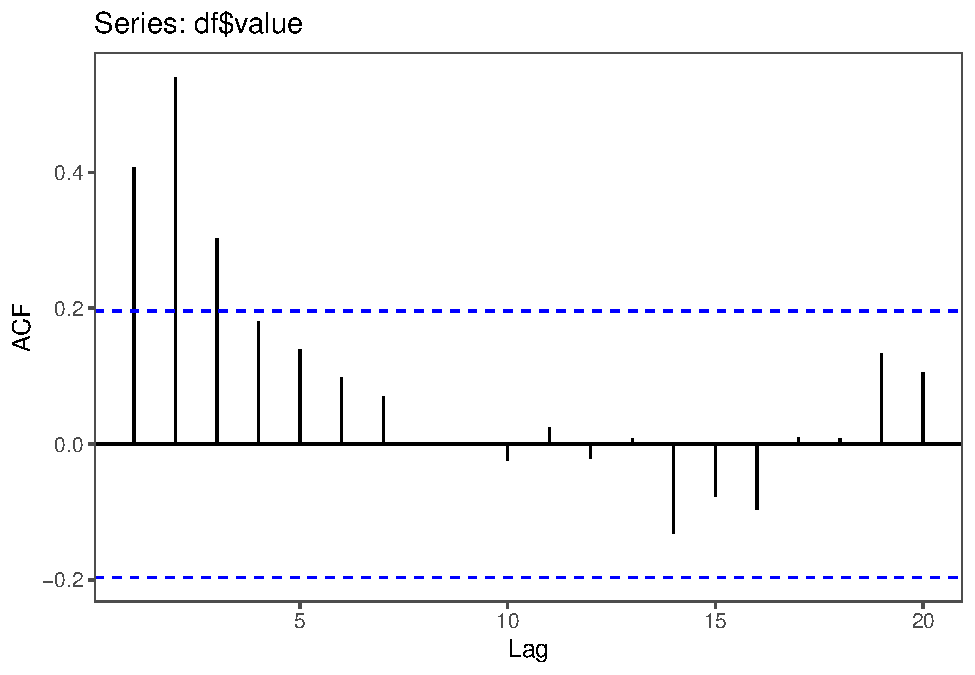
\includegraphics{Econo2_P4_files/figure-latex/plots-3} \end{center}

\begin{Shaded}
	\begin{Highlighting}[]
		\NormalTok{faclt}
	\end{Highlighting}
\end{Shaded}

\begin{center}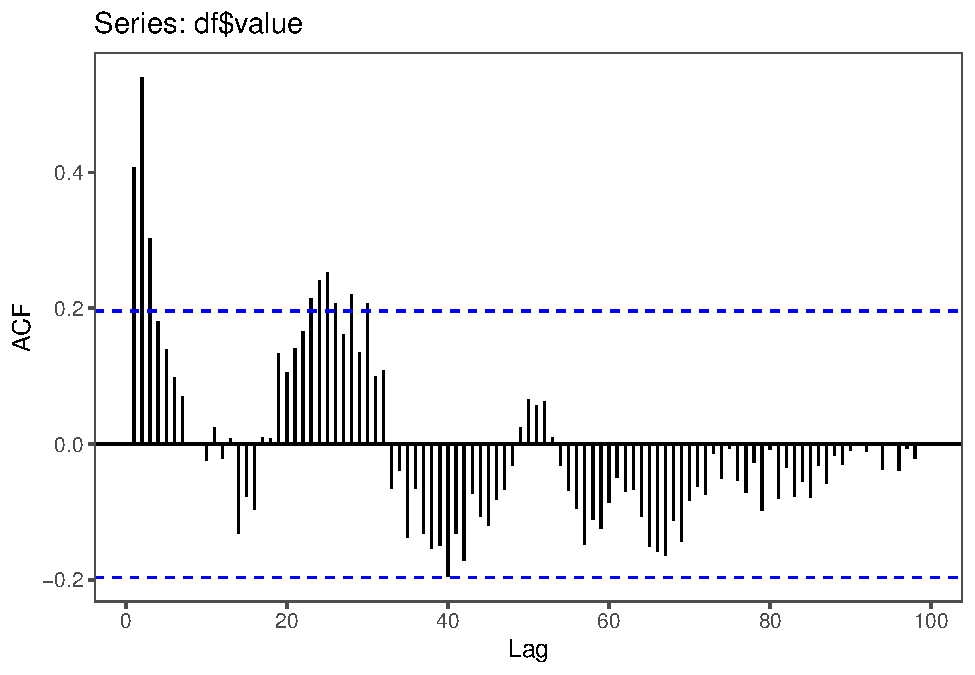
\includegraphics{Econo2_P4_files/figure-latex/plots-4} \end{center}

\begin{Shaded}
	\begin{Highlighting}[]
		\NormalTok{facpst}
	\end{Highlighting}
\end{Shaded}

\begin{center}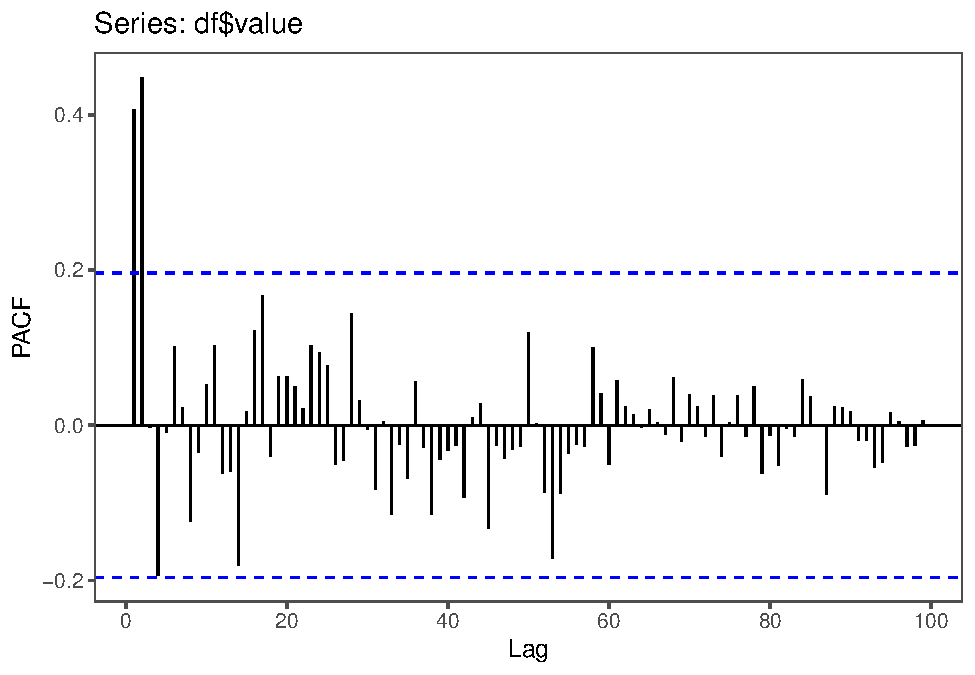
\includegraphics{Econo2_P4_files/figure-latex/plots-5} \end{center}

\begin{Shaded}
	\begin{Highlighting}[]
		\NormalTok{facplt}
	\end{Highlighting}
\end{Shaded}

\begin{center}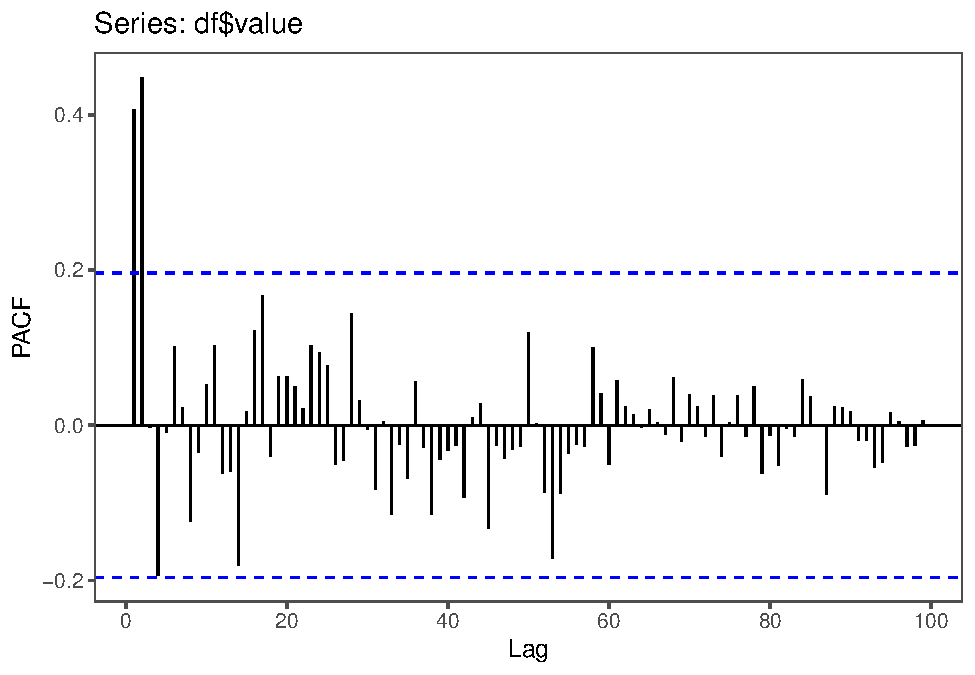
\includegraphics{Econo2_P4_files/figure-latex/plots-6} \end{center}

We'll now use the function \emph{auto.arima} from the package
\emph{forecast} to identify and estimate the model.

\begin{Shaded}
	\begin{Highlighting}[]
		\NormalTok{aa_model <-}\StringTok{ }\KeywordTok{auto.arima}\NormalTok{(df}\OperatorTok{$}\NormalTok{value, }\DataTypeTok{num.cores =} \DecValTok{24}\NormalTok{, }\DataTypeTok{max.d =} \DecValTok{0}\NormalTok{, }\DataTypeTok{stepwise =}\NormalTok{ F)}
		
		\KeywordTok{summary}\NormalTok{(aa_model)}
	\end{Highlighting}
\end{Shaded}

\begin{verbatim}
	## Series: df$value 
	## ARIMA(0,0,3) with non-zero mean 
	## 
	## Coefficients:
	##          ma1     ma2     ma3    mean
	##       0.1814  0.6647  0.4001  5.8982
	## s.e.  0.0852  0.0750  0.0949  0.0562
	## 
	## sigma^2 estimated as 0.0667:  log likelihood=-5.42
	## AIC=20.85   AICc=21.49   BIC=33.88
	## 
	## Training set error measures:
	##                        ME      RMSE       MAE        MPE     MAPE      MASE
	## Training set -0.002315954 0.2530428 0.2131067 -0.2268814 3.612855 0.7314965
	##                    ACF1
	## Training set 0.03868106
\end{verbatim}

\begin{Shaded}
	\begin{Highlighting}[]
		\KeywordTok{print}\NormalTok{(}\StringTok{"t-values: "}\NormalTok{)}
	\end{Highlighting}
\end{Shaded}

\begin{verbatim}
	## [1] "t-values: "
\end{verbatim}

\begin{Shaded}
	\begin{Highlighting}[]
		\NormalTok{aa_t <-}\StringTok{ }\KeywordTok{matrix}\NormalTok{(}\OtherTok{NA}\NormalTok{, }\DataTypeTok{nrow =}\NormalTok{ aa_model}\OperatorTok{$}\NormalTok{arma[}\DecValTok{1}\NormalTok{] }\OperatorTok{+}\StringTok{ }\NormalTok{aa_model}\OperatorTok{$}\NormalTok{arma[}\DecValTok{2}\NormalTok{])}
		
		\ControlFlowTok{for}\NormalTok{ (i }\ControlFlowTok{in} \KeywordTok{c}\NormalTok{(}\DecValTok{1}\OperatorTok{:}\DecValTok{4}\NormalTok{)) \{}
		
		\NormalTok{    aa_t[i] <-}\StringTok{ }\NormalTok{aa_model}\OperatorTok{$}\NormalTok{coef[i]}\OperatorTok{/}\KeywordTok{sqrt}\NormalTok{(aa_model}\OperatorTok{$}\NormalTok{var.coef[i, i])}
		
		\NormalTok{\}}
		
		\NormalTok{aa_t <-}\StringTok{ }\KeywordTok{data.frame}\NormalTok{(aa_t)}
		
		\NormalTok{aa_t}
	\end{Highlighting}
\end{Shaded}

\begin{verbatim}
	##         aa_t
	## 1   2.128691
	## 2   8.861580
	## 3   4.216481
	## 4 105.004537
\end{verbatim}

\begin{Shaded}
	\begin{Highlighting}[]
		\NormalTok{aa_q <-}\StringTok{ }\KeywordTok{Box.test}\NormalTok{(aa_model}\OperatorTok{$}\NormalTok{residuals, }\DataTypeTok{lag =}\NormalTok{ aa_model}\OperatorTok{$}\NormalTok{arma[}\DecValTok{1}\NormalTok{] }\OperatorTok{+}\StringTok{ }
		\StringTok{    }\NormalTok{aa_model}\OperatorTok{$}\NormalTok{arma[}\DecValTok{2}\NormalTok{])}
		\NormalTok{aa_q}
	\end{Highlighting}
\end{Shaded}

\begin{verbatim}
	## 
	##  Box-Pierce test
	## 
	## data:  aa_model$residuals
	## X-squared = 0.35002, df = 3, p-value = 0.9504
\end{verbatim}

\begin{Shaded}
	\begin{Highlighting}[]
		\NormalTok{criteria <-}\StringTok{ }\KeywordTok{matrix}\NormalTok{(}\OtherTok{NA}\NormalTok{, }\DataTypeTok{nrow =} \DecValTok{1}\NormalTok{, }\DataTypeTok{ncol =} \DecValTok{3}\NormalTok{)}
		
		\NormalTok{aa_criteria <-}\StringTok{ }\KeywordTok{data.frame}\NormalTok{(}\StringTok{"MA(3)*"}\NormalTok{, aa_model}\OperatorTok{$}\NormalTok{aic, aa_model}\OperatorTok{$}\NormalTok{bic)}
		
		\KeywordTok{names}\NormalTok{(aa_criteria) <-}\StringTok{ }\KeywordTok{c}\NormalTok{(}\StringTok{"Model"}\NormalTok{, }\StringTok{"AIC"}\NormalTok{, }\StringTok{"BIC"}\NormalTok{)}
		
		\NormalTok{aa_criteria}
	\end{Highlighting}
\end{Shaded}

\begin{verbatim}
	##    Model      AIC      BIC
	## 1 MA(3)* 20.84963 33.87549
\end{verbatim}

\begin{Shaded}
	\begin{Highlighting}[]
		\NormalTok{fac_e <-}\StringTok{ }\KeywordTok{ggAcf}\NormalTok{(aa_model}\OperatorTok{$}\NormalTok{residuals, }\DataTypeTok{type =} \StringTok{"correlation"}\NormalTok{, }\DataTypeTok{lag.max =} \DecValTok{20}\NormalTok{, }
		\DataTypeTok{plot =}\NormalTok{ T) }\OperatorTok{+}\StringTok{ }\KeywordTok{theme_few}\NormalTok{()}
		
		\NormalTok{facp_e <-}\StringTok{ }\KeywordTok{ggPacf}\NormalTok{(aa_model}\OperatorTok{$}\NormalTok{residuals, }\DataTypeTok{type =} \StringTok{"correlation"}\NormalTok{, }\DataTypeTok{lag.max =} \DecValTok{20}\NormalTok{, }
		\DataTypeTok{plot =}\NormalTok{ T) }\OperatorTok{+}\StringTok{ }\KeywordTok{theme_few}\NormalTok{()}
	\end{Highlighting}
\end{Shaded}

\begin{verbatim}
	## Warning: Ignoring unknown parameters: type
\end{verbatim}

\begin{Shaded}
	\begin{Highlighting}[]
		\NormalTok{fac_e}
	\end{Highlighting}
\end{Shaded}

\begin{center}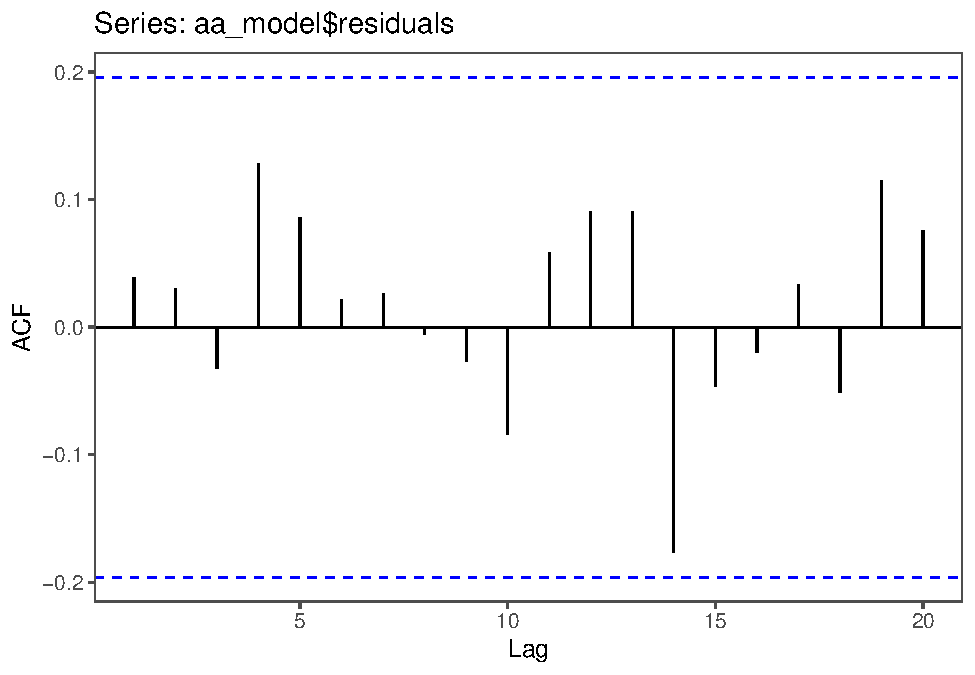
\includegraphics{Econo2_P4_files/figure-latex/estimation autoarima-1} \end{center}

\begin{Shaded}
	\begin{Highlighting}[]
		\NormalTok{facp_e}
	\end{Highlighting}
\end{Shaded}

\begin{center}\includegraphics{Econo2_P4_files/figure-latex/estimation autoarima-2} \end{center}

\begin{Shaded}
	\begin{Highlighting}[]
		\KeywordTok{mean}\NormalTok{(aa_model}\OperatorTok{$}\NormalTok{residuals)}
	\end{Highlighting}
\end{Shaded}

\begin{verbatim}
	## [1] -0.002315954
\end{verbatim}

The results of \emph{auto.arima} imply that the best model is an
ARMA(0,3) -- i.e., a MA(3):
\[ y_t = c +  + \theta_1 \varepsilon_{t-1} + \theta_2 \varepsilon_{t-2}+ \theta_3 \varepsilon_{t-3} + \varepsilon_t, \hspace{1em} \varepsilon_t \sim wn(0, \sigma^2)\]

Furthermore, the Q-statistic \emph{(Box.test)} seems to indicate that
\(\varepsilon_t\) is truly white noise.

\section{Cross-validation}

Let's now cross-validate or model. This will now be done manually;
afterwards, an automatized version from \emph{fpp} shall be presented.

Let \(h := 5\); \(frac = 0.2\). \(T\) is the size of our sample; \(k\)
is the \emph{training} database. The remainder shall be used for testing
purposes.

As we have discovered previously, \emph{auto.arima} yields a
\textbf{MA(3)} model. It will now be used.

\begin{Shaded}
	\begin{Highlighting}[]
		\NormalTok{h <-}\StringTok{ }\DecValTok{5}
		
		\NormalTok{frac <-}\StringTok{ }\FloatTok{0.2}
		
		\NormalTok{T <-}\StringTok{ }\KeywordTok{length}\NormalTok{(df}\OperatorTok{$}\NormalTok{value)}
		
		\NormalTok{k <-}\StringTok{ }\KeywordTok{floor}\NormalTok{((}\DecValTok{1} \OperatorTok{-}\StringTok{ }\NormalTok{frac) }\OperatorTok{*}\StringTok{ }\NormalTok{T)}
		
		\CommentTok{# Estimating MA(3) with k = 80}
		\NormalTok{fit <-}\StringTok{ }\KeywordTok{Arima}\NormalTok{(df}\OperatorTok{$}\NormalTok{value[}\DecValTok{1}\OperatorTok{:}\NormalTok{k], }\DataTypeTok{order =} \KeywordTok{c}\NormalTok{(}\DecValTok{0}\NormalTok{, }\DecValTok{0}\NormalTok{, }\DecValTok{3}\NormalTok{))}
		
		\CommentTok{# Generating predictions from the model}
		\NormalTok{pred <-}\StringTok{ }\KeywordTok{predict}\NormalTok{(fit, }\DataTypeTok{n.ahead =}\NormalTok{ h)}
		
		\CommentTok{# Calculating errors between the predicted values of the}
		\CommentTok{# model and the actual values of the testing database}
		
		\NormalTok{e <-}\StringTok{ }\NormalTok{df}\OperatorTok{$}\NormalTok{value[(k }\OperatorTok{+}\StringTok{ }\NormalTok{h)] }\OperatorTok{-}\StringTok{ }\NormalTok{pred}\OperatorTok{$}\NormalTok{pred[h]}
		
		\NormalTok{e}
	\end{Highlighting}
\end{Shaded}

\begin{verbatim}
	## [1] -0.1951299
\end{verbatim}

Let's now update our training database iteratively with a for loop.

\begin{Shaded}
	\begin{Highlighting}[]
		\NormalTok{e <-}\StringTok{ }\KeywordTok{matrix}\NormalTok{(}\OtherTok{NA}\NormalTok{, }\DataTypeTok{nrow =} \DecValTok{100}\NormalTok{)}
		
		\CommentTok{# Updating the model}
		
		\ControlFlowTok{for}\NormalTok{ (i }\ControlFlowTok{in}\NormalTok{ k}\OperatorTok{:}\NormalTok{(T }\OperatorTok{-}\StringTok{ }\NormalTok{h)) \{}
		
		\NormalTok{    fit <-}\StringTok{ }\KeywordTok{Arima}\NormalTok{(df}\OperatorTok{$}\NormalTok{value[}\DecValTok{1}\OperatorTok{:}\NormalTok{i], }\DataTypeTok{order =} \KeywordTok{c}\NormalTok{(}\DecValTok{0}\NormalTok{, }\DecValTok{0}\NormalTok{, }\DecValTok{3}\NormalTok{))}
		
		\NormalTok{    pred <-}\StringTok{ }\KeywordTok{predict}\NormalTok{(fit, }\DataTypeTok{n.ahead =}\NormalTok{ h)}
		
		\NormalTok{    e[i, }\DecValTok{1}\NormalTok{] <-}\StringTok{ }\NormalTok{df}\OperatorTok{$}\NormalTok{value[(i }\OperatorTok{+}\StringTok{ }\NormalTok{h)] }\OperatorTok{-}\StringTok{ }\NormalTok{pred}\OperatorTok{$}\NormalTok{pred[h]}
		
		\NormalTok{\}}
	\end{Highlighting}
\end{Shaded}

With the matrix \emph{e} in hands, we can now calculate MSE:

\begin{Shaded}
	\begin{Highlighting}[]
		\NormalTok{mse <-}\StringTok{ }\KeywordTok{mean}\NormalTok{(e}\OperatorTok{^}\DecValTok{2}\NormalTok{, }\DataTypeTok{na.rm =}\NormalTok{ T)}
	\end{Highlighting}
\end{Shaded}

This procedure can now be used to compare other models against the model
from \emph{auto.arima}.

\begin{Shaded}
	\begin{Highlighting}[]
		\NormalTok{max_p <-}\StringTok{ }\DecValTok{5}
		
		\NormalTok{max_q <-}\StringTok{ }\DecValTok{5}
		
		\NormalTok{e <-}\StringTok{ }\KeywordTok{matrix}\NormalTok{(}\OtherTok{NA}\NormalTok{, }\DataTypeTok{nrow =} \DecValTok{100}\NormalTok{, }\DataTypeTok{ncol =}\NormalTok{ (max_p }\OperatorTok{+}\StringTok{ }\DecValTok{1}\NormalTok{) }\OperatorTok{*}\StringTok{ }\NormalTok{(max_q }\OperatorTok{+}\StringTok{ }\DecValTok{1}\NormalTok{))}
		
		\NormalTok{pred <-}\StringTok{ }\KeywordTok{vector}\NormalTok{(}\StringTok{"list"}\NormalTok{, (max_p }\OperatorTok{+}\StringTok{ }\DecValTok{1}\NormalTok{) }\OperatorTok{*}\StringTok{ }\NormalTok{(max_q }\OperatorTok{+}\StringTok{ }\DecValTok{1}\NormalTok{))}
		
		\NormalTok{fit <-}\StringTok{ }\KeywordTok{vector}\NormalTok{(}\StringTok{"list"}\NormalTok{, (max_p }\OperatorTok{+}\StringTok{ }\DecValTok{1}\NormalTok{) }\OperatorTok{*}\StringTok{ }\NormalTok{(max_q }\OperatorTok{+}\StringTok{ }\DecValTok{1}\NormalTok{))}
		
		\CommentTok{# Updating the model}
		\ControlFlowTok{for}\NormalTok{ (u }\ControlFlowTok{in} \DecValTok{0}\OperatorTok{:}\NormalTok{max_q) \{}
		
		\ControlFlowTok{for}\NormalTok{ (j }\ControlFlowTok{in} \DecValTok{0}\OperatorTok{:}\NormalTok{max_p) \{}
		
		
		\ControlFlowTok{for}\NormalTok{ (i }\ControlFlowTok{in}\NormalTok{ k}\OperatorTok{:}\NormalTok{(T }\OperatorTok{-}\StringTok{ }\NormalTok{h)) \{}
		
		\NormalTok{            fit[[(((max_p }\OperatorTok{+}\StringTok{ }\DecValTok{1}\NormalTok{) }\OperatorTok{*}\StringTok{ }\NormalTok{j) }\OperatorTok{+}\StringTok{ }\NormalTok{u }\OperatorTok{+}\StringTok{ }\DecValTok{1}\NormalTok{)]] <-}\StringTok{ }\KeywordTok{Arima}\NormalTok{(df}\OperatorTok{$}\NormalTok{value[}\DecValTok{1}\OperatorTok{:}\NormalTok{i], }
		\DataTypeTok{order =} \KeywordTok{c}\NormalTok{(j, }\DecValTok{0}\NormalTok{, u))}
		
		\CommentTok{# fit <- append(fit, Arima(df$value[1:i], order = c(j,0,u)))}
		
		\CommentTok{# pred <- append(pred, predict(fit[[(j+u)]], n.ahead = h))}
		
		\NormalTok{            pred[[(((max_p }\OperatorTok{+}\StringTok{ }\DecValTok{1}\NormalTok{) }\OperatorTok{*}\StringTok{ }\NormalTok{j) }\OperatorTok{+}\StringTok{ }\NormalTok{u }\OperatorTok{+}\StringTok{ }\DecValTok{1}\NormalTok{)]] <-}\StringTok{ }\KeywordTok{predict}\NormalTok{(fit[[(((max_p }\OperatorTok{+}\StringTok{ }
		\StringTok{                }\DecValTok{1}\NormalTok{) }\OperatorTok{*}\StringTok{ }\NormalTok{j) }\OperatorTok{+}\StringTok{ }\NormalTok{u }\OperatorTok{+}\StringTok{ }\DecValTok{1}\NormalTok{)]], }\DataTypeTok{n.ahead =}\NormalTok{ h)}
		
		\NormalTok{            e[i, (((max_p }\OperatorTok{+}\StringTok{ }\DecValTok{1}\NormalTok{) }\OperatorTok{*}\StringTok{ }\NormalTok{j) }\OperatorTok{+}\StringTok{ }\NormalTok{u }\OperatorTok{+}\StringTok{ }\DecValTok{1}\NormalTok{)] <-}\StringTok{ }\NormalTok{df}\OperatorTok{$}\NormalTok{value[(i }\OperatorTok{+}\StringTok{ }
		\StringTok{                }\NormalTok{h)] }\OperatorTok{-}\StringTok{ }\NormalTok{pred[[(((max_p }\OperatorTok{+}\StringTok{ }\DecValTok{1}\NormalTok{) }\OperatorTok{*}\StringTok{ }\NormalTok{j) }\OperatorTok{+}\StringTok{ }\NormalTok{u }\OperatorTok{+}\StringTok{ }\DecValTok{1}\NormalTok{)]]}\OperatorTok{$}\NormalTok{pred[h]}
		
		\NormalTok{        \}}
		
		\NormalTok{    \}}
		
		\NormalTok{\}}
		
		\NormalTok{mse <-}\StringTok{ }\KeywordTok{matrix}\NormalTok{(}\OtherTok{NA}\NormalTok{, }\DataTypeTok{nrow =}\NormalTok{ ((max_p }\OperatorTok{+}\StringTok{ }\DecValTok{1}\NormalTok{) }\OperatorTok{*}\StringTok{ }\NormalTok{(max_q }\OperatorTok{+}\StringTok{ }\DecValTok{1}\NormalTok{)), }\DataTypeTok{ncol =} \DecValTok{1}\NormalTok{)}
		
		
		
		
		\NormalTok{mse <-}\StringTok{ }\KeywordTok{colMeans}\NormalTok{(e}\OperatorTok{^}\DecValTok{2}\NormalTok{, }\DataTypeTok{na.rm =}\NormalTok{ T)}
		
		\NormalTok{mse}
	\end{Highlighting}
\end{Shaded}

\begin{verbatim}
	##  [1] 0.1357466 0.1354001 0.1368083 0.1374243 0.1376508 0.1441940 0.1347115
	##  [8] 0.1269779 0.1347789 0.1373465 0.1398588 0.1436175 0.1313779 0.1315448
	## [15] 0.1435805 0.1355649 0.1421277 0.1335153 0.1316765 0.1333955 0.1400838
	## [22] 0.1427467 0.1473227 0.1347447 0.1320856 0.1333025 0.1354734 0.1341742
	## [29] 0.1380676 0.1357880 0.1346228 0.1382810 0.1319484 0.1308446 0.1382417
	## [36] 0.1327046
\end{verbatim}

\begin{Shaded}
	\begin{Highlighting}[]
		\NormalTok{optimal_index <-}\StringTok{ }\KeywordTok{which.min}\NormalTok{(mse)}
		
		\NormalTok{cv_model <-}\StringTok{ }\NormalTok{fit[[optimal_index]]}
		
		\KeywordTok{summary}\NormalTok{(cv_model)}
	\end{Highlighting}
\end{Shaded}

\begin{verbatim}
	## Series: df$value[1:i] 
	## ARIMA(1,0,1) with non-zero mean 
	## 
	## Coefficients:
	##          ar1      ma1    mean
	##       0.8253  -0.4888  5.9125
	## s.e.  0.0814   0.1118  0.0815
	## 
	## sigma^2 estimated as 0.08209:  log likelihood=-14.72
	## AIC=37.43   AICc=37.88   BIC=47.65
	## 
	## Training set error measures:
	##                        ME      RMSE       MAE        MPE     MAPE      MASE
	## Training set -0.002725722 0.2819456 0.2228183 -0.2756862 3.787114 0.7600473
	##                    ACF1
	## Training set -0.1279409
\end{verbatim}

The cross-validation method constructed above yielded an ARMA(1,1):
\[ y_t = c + \phi_1 y_{t-1} +  + \theta_1 \varepsilon_{t-1} + \varepsilon_t, \hspace{1em} \varepsilon_t \sim wn(0, \sigma^2)\]

\begin{Shaded}
	\begin{Highlighting}[]
		\NormalTok{cv_fc <-}\StringTok{ }\KeywordTok{forecast}\NormalTok{(cv_model, }\DataTypeTok{h =}\NormalTok{ h)}
		
		\KeywordTok{autoplot}\NormalTok{(cv_fc)}
	\end{Highlighting}
\end{Shaded}

\begin{center}\includegraphics{Econo2_P4_files/figure-latex/forecast cv plot-1} \end{center}

\section{Bootstrapping}

Now, let's proceed to \emph{bootstrapping}. It envolves the following
steps:

\begin{enumerate}
	\item \begin{itemize}
		\item Estimate ARMA(p,q)
		$$ Y_t = c + \sum_{j=1}^p \phi_j Y_{t-j} + \sum_{j=1}^q \theta_j \varepsilon_{t-j} + \varepsilon_t$$
		
		\item Calculate the residuals of the regression:
		$$ \hat{\varepsilon}_t := Y_t - (\hat{c} + \sum_{j=1}^p \hat{\phi}_j Y_{t-j} + \sum_{j=1}^q \hat{\theta}_j \varepsilon_{t-j})$$
		
		\item If the residuals do not have mean 0, create the centered residuals:
		$$ \tilde{\varepsilon}_t = \hat{\varepsilon}_t - \frac{1}{t} \sum_{t=1}^T \hat{\varepsilon}_t$$
	\end{itemize}
	
	\item \begin{itemize}
		\item Select at random, with replacement, a sample with $T + m$ elements, $m >> 0$:
		$$\{\varepsilon^*_1, ..., \varepsilon^*_{T+m}\}$$
		\item Create a series $\{Y^*_t\}_{t=1}^{T+m}$:
		$$ Y_t^* = Y_t, 1 \leq t \leq max(p,q) $$
		$$ Y_t^* = \hat{c} + \sum_{j=1}^p \hat{\phi}_j Y_{t-j} + \sum_{j=1}^q \hat{\theta}_j \varepsilon_{t-j}^* + \varepsilon_t^*, max(p,q) < t \leq T + m $$
	\end{itemize}
	\item \begin{itemize}
		\item Using the simulated sample $\{Y^*_t\}_{t=1}^{T+m}$, create a forecast for $h >0$ periods using the estimated coefficients \textit{obtained with the real sample}.
		\item This yields a vector of dimension $h$ containing the forecasts in the form:
		$$(\hat{Y}^*_{T+1}, ..., \hat{Y}^*_{T+h})$$ 
		\item Repeat steps 2 and 3 for $S$ times. Create a matrix with the results.
		\item This yields a S x h matrix where each row is equal to the aforementioned vector.
	\end{itemize}
\end{enumerate}

We'll use, again, the optimal model from \emph{auto.arima}, MA(3):

\[ y_t = c +  + \theta_1 \varepsilon_{t-1} + \theta_2 \varepsilon_{t-2}+ \theta_3 \varepsilon_{t-3} + \varepsilon_t, \hspace{1em} \varepsilon_t \sim wn(0, \sigma^2)\]

\begin{Shaded}
	\begin{Highlighting}[]
		\NormalTok{S <-}\StringTok{ }\DecValTok{1000}
		
		\NormalTok{m <-}\StringTok{ }\DecValTok{100}
		
		
		
		\NormalTok{optimal_p <-}\StringTok{ }\NormalTok{aa_model}\OperatorTok{$}\NormalTok{arma[}\DecValTok{1}\NormalTok{]}
		
		\NormalTok{optimal_q <-}\StringTok{ }\NormalTok{aa_model}\OperatorTok{$}\NormalTok{arma[}\DecValTok{2}\NormalTok{]}
		
		\NormalTok{e_sample <-}\StringTok{ }\KeywordTok{data.frame}\NormalTok{(}\KeywordTok{matrix}\NormalTok{(}\OtherTok{NA}\NormalTok{, }\DataTypeTok{nrow =}\NormalTok{ S, }\DataTypeTok{ncol =}\NormalTok{ (}\KeywordTok{length}\NormalTok{(df}\OperatorTok{$}\NormalTok{value) }\OperatorTok{+}\StringTok{ }
		\StringTok{    }\NormalTok{m)))}
		
		\NormalTok{y_star <-}\StringTok{ }\KeywordTok{data.frame}\NormalTok{(}\KeywordTok{matrix}\NormalTok{(}\OtherTok{NA}\NormalTok{, }\DataTypeTok{nrow =}\NormalTok{ S, }\DataTypeTok{ncol =}\NormalTok{ (}\KeywordTok{length}\NormalTok{(df}\OperatorTok{$}\NormalTok{value) }\OperatorTok{+}\StringTok{ }
		\StringTok{    }\NormalTok{m }\OperatorTok{+}\StringTok{ }\KeywordTok{max}\NormalTok{(aa_model}\OperatorTok{$}\NormalTok{arma[}\DecValTok{1}\NormalTok{], aa_model}\OperatorTok{$}\NormalTok{arma[}\DecValTok{2}\NormalTok{]))))}
		
		\NormalTok{arima_star <-}\StringTok{ }\KeywordTok{data.frame}\NormalTok{(}\KeywordTok{matrix}\NormalTok{(}\OtherTok{NA}\NormalTok{, }\DataTypeTok{nrow =}\NormalTok{ S, }\DataTypeTok{ncol =}\NormalTok{ (}\KeywordTok{length}\NormalTok{(df}\OperatorTok{$}\NormalTok{value) }\OperatorTok{+}\StringTok{ }
		\StringTok{    }\NormalTok{m }\OperatorTok{+}\StringTok{ }\KeywordTok{max}\NormalTok{(aa_model}\OperatorTok{$}\NormalTok{arma[}\DecValTok{1}\NormalTok{], aa_model}\OperatorTok{$}\NormalTok{arma[}\DecValTok{2}\NormalTok{]))))}
		
		
		\ControlFlowTok{for}\NormalTok{ (i }\ControlFlowTok{in} \DecValTok{1}\OperatorTok{:}\NormalTok{S) \{}
		
		\NormalTok{    e_sample[i] <-}\StringTok{ }\KeywordTok{sample}\NormalTok{(aa_model}\OperatorTok{$}\NormalTok{residuals, }\DataTypeTok{replace =}\NormalTok{ T, }\DataTypeTok{size =}\NormalTok{ (}\KeywordTok{length}\NormalTok{(df}\OperatorTok{$}\NormalTok{value) }\OperatorTok{+}\StringTok{ }
		\StringTok{        }\NormalTok{m))}
		
		\NormalTok{\}}
		
		\ControlFlowTok{for}\NormalTok{ (i }\ControlFlowTok{in} \DecValTok{1}\OperatorTok{:}\NormalTok{S) \{}
		
		\ControlFlowTok{for}\NormalTok{ (j }\ControlFlowTok{in}\NormalTok{ ((aa_model}\OperatorTok{$}\NormalTok{arma[}\DecValTok{1}\NormalTok{] }\OperatorTok{+}\StringTok{ }\NormalTok{aa_model}\OperatorTok{$}\NormalTok{arma[}\DecValTok{2}\NormalTok{] }\OperatorTok{+}\StringTok{ }\DecValTok{1}\NormalTok{)}\OperatorTok{:}\NormalTok{(}\KeywordTok{length}\NormalTok{(df}\OperatorTok{$}\NormalTok{value) }\OperatorTok{+}\StringTok{ }
		\StringTok{        }\NormalTok{m))) \{}
		
		\NormalTok{        arima_star[i, j] <-}\StringTok{ }\NormalTok{(aa_model}\OperatorTok{$}\NormalTok{coef[}\DecValTok{4}\NormalTok{] }\OperatorTok{+}\StringTok{ }\NormalTok{(aa_model}\OperatorTok{$}\NormalTok{coef[}\DecValTok{1}\NormalTok{] }\OperatorTok{*}\StringTok{ }
		\StringTok{            }\NormalTok{e_sample[i, j }\OperatorTok{-}\StringTok{ }\DecValTok{1}\NormalTok{]) }\OperatorTok{+}\StringTok{ }\NormalTok{(aa_model}\OperatorTok{$}\NormalTok{coef[}\DecValTok{2}\NormalTok{] }\OperatorTok{*}\StringTok{ }\NormalTok{e_sample[i, }
		\NormalTok{            j }\OperatorTok{-}\StringTok{ }\DecValTok{2}\NormalTok{]) }\OperatorTok{+}\StringTok{ }\NormalTok{(aa_model}\OperatorTok{$}\NormalTok{coef[}\DecValTok{3}\NormalTok{] }\OperatorTok{*}\StringTok{ }\NormalTok{e_sample[i, j }\OperatorTok{-}\StringTok{ }\DecValTok{3}\NormalTok{]) }\OperatorTok{+}\StringTok{ }
		\StringTok{            }\NormalTok{e_sample[i, j])}
		
		\NormalTok{    \}}
		
		\NormalTok{\}}
		
		
		\NormalTok{y_fixed <-}\StringTok{ }\KeywordTok{data.frame}\NormalTok{(}\KeywordTok{matrix}\NormalTok{(}\OtherTok{NA}\NormalTok{, }\DataTypeTok{nrow =}\NormalTok{ S, }\DataTypeTok{ncol =}\NormalTok{ (aa_model}\OperatorTok{$}\NormalTok{arma[}\DecValTok{1}\NormalTok{] }\OperatorTok{+}\StringTok{ }
		\StringTok{    }\NormalTok{aa_model}\OperatorTok{$}\NormalTok{arma[}\DecValTok{2}\NormalTok{])))}
		
		\ControlFlowTok{for}\NormalTok{ (i }\ControlFlowTok{in} \DecValTok{1}\OperatorTok{:}\NormalTok{S) \{}
		\NormalTok{    y_fixed[i, }\DecValTok{1}\NormalTok{] <-}\StringTok{ }\KeywordTok{data.frame}\NormalTok{(df}\OperatorTok{$}\NormalTok{value[}\DecValTok{1}\NormalTok{])}
		\NormalTok{    y_fixed[i, }\DecValTok{2}\NormalTok{] <-}\StringTok{ }\KeywordTok{data.frame}\NormalTok{(df}\OperatorTok{$}\NormalTok{value[}\DecValTok{2}\NormalTok{])}
		\NormalTok{    y_fixed[i, }\DecValTok{3}\NormalTok{] <-}\StringTok{ }\KeywordTok{data.frame}\NormalTok{(df}\OperatorTok{$}\NormalTok{value[}\DecValTok{3}\NormalTok{])}
		\NormalTok{\}}
		
		
		\NormalTok{y_star <-}\StringTok{ }\KeywordTok{data.frame}\NormalTok{(y_fixed, arima_star[, }\OperatorTok{-}\NormalTok{(}\DecValTok{1}\OperatorTok{:}\DecValTok{3}\NormalTok{)])}
		
		\NormalTok{y_m <-}\StringTok{ }\NormalTok{y_star[, }\OperatorTok{-}\NormalTok{(}\DecValTok{1}\OperatorTok{:}\DecValTok{100}\NormalTok{)]}
		
		\NormalTok{y_m <-}\StringTok{ }\NormalTok{y_m[, }\OperatorTok{-}\NormalTok{(}\DecValTok{101}\OperatorTok{:}\DecValTok{103}\NormalTok{)]}
		
		\NormalTok{y_mt <-}\StringTok{ }\KeywordTok{t}\NormalTok{(y_m)}
		
		\NormalTok{y_matrix <-}\StringTok{ }\KeywordTok{as.matrix}\NormalTok{(y_m)}
	\end{Highlighting}
\end{Shaded}

\begin{Shaded}
	\begin{Highlighting}[]
		\NormalTok{fc_list <-}\StringTok{ }\KeywordTok{vector}\NormalTok{(}\StringTok{"list"}\NormalTok{, S)}
		
		\ControlFlowTok{for}\NormalTok{ (i }\ControlFlowTok{in} \DecValTok{1}\OperatorTok{:}\NormalTok{S) \{}
		
		\NormalTok{    fc_list[[i]] <-}\StringTok{ }\KeywordTok{forecast}\NormalTok{(}\KeywordTok{ts}\NormalTok{(y_matrix[i, ]), }\DataTypeTok{model =}\NormalTok{ aa_model, }
		\DataTypeTok{h =} \DecValTok{5}\NormalTok{)}
		
		\NormalTok{\}}
		
		\NormalTok{fc_list[[}\DecValTok{1}\NormalTok{]]}
	\end{Highlighting}
\end{Shaded}

\begin{verbatim}
	##     Point Forecast    Lo 80    Hi 80    Lo 95    Hi 95
	## 101       5.880900 5.549926 6.211875 5.374719 6.387082
	## 102       5.869038 5.532663 6.205413 5.354597 6.383479
	## 103       5.841494 5.439567 6.243421 5.226800 6.456189
	## 104       5.898184 5.475000 6.321368 5.250980 6.545387
	## 105       5.898184 5.475000 6.321368 5.250980 6.545387
\end{verbatim}

\begin{Shaded}
	\begin{Highlighting}[]
		\NormalTok{fc_mean <-}\StringTok{ }\KeywordTok{data.frame}\NormalTok{(}\KeywordTok{matrix}\NormalTok{(}\OtherTok{NA}\NormalTok{, }\DataTypeTok{nrow =}\NormalTok{ S, }\DataTypeTok{ncol =} \DecValTok{5}\NormalTok{))}
		
		\ControlFlowTok{for}\NormalTok{ (i }\ControlFlowTok{in} \DecValTok{1}\OperatorTok{:}\NormalTok{S) \{}
		
		\NormalTok{    fc_mean[i, ] <-}\StringTok{ }\NormalTok{fc_list[[i]]}\OperatorTok{$}\NormalTok{mean}
		
		\NormalTok{\}}
	\end{Highlighting}
\end{Shaded}

\begin{Shaded}
	\begin{Highlighting}[]
		\KeywordTok{head}\NormalTok{(fc_mean)}
	\end{Highlighting}
\end{Shaded}

\begin{verbatim}
	##         X1       X2       X3       X4       X5
	## 1 5.880900 5.869038 5.841494 5.898184 5.898184
	## 2 5.734428 5.543250 5.786803 5.898184 5.898184
	## 3 5.728049 5.722659 5.832225 5.898184 5.898184
	## 4 5.844103 5.943213 5.958997 5.898184 5.898184
	## 5 5.550780 5.518844 5.732659 5.898184 5.898184
	## 6 5.742853 5.863462 5.848949 5.898184 5.898184
\end{verbatim}

\begin{Shaded}
	\begin{Highlighting}[]
		\NormalTok{hist_x1 <-}\StringTok{ }\KeywordTok{ggplot}\NormalTok{(}\DataTypeTok{data =}\NormalTok{ fc_mean, }\KeywordTok{aes}\NormalTok{(}\DataTypeTok{x =}\NormalTok{ X1)) }\OperatorTok{+}\StringTok{ }\KeywordTok{geom_histogram}\NormalTok{(}\DataTypeTok{bins =} \DecValTok{40}\NormalTok{) }\OperatorTok{+}\StringTok{ }
		\StringTok{    }\KeywordTok{theme_few}\NormalTok{()}
		\NormalTok{hist_x1}
	\end{Highlighting}
\end{Shaded}

\begin{center}\includegraphics{Econo2_P4_files/figure-latex/mean ic-1} \end{center}

\begin{Shaded}
	\begin{Highlighting}[]
		\NormalTok{qq_x1 <-}\StringTok{ }\KeywordTok{qqnorm}\NormalTok{(fc_mean}\OperatorTok{$}\NormalTok{X1)}
		\KeywordTok{qqline}\NormalTok{(fc_mean}\OperatorTok{$}\NormalTok{X1)}
	\end{Highlighting}
\end{Shaded}

\begin{center}\includegraphics{Econo2_P4_files/figure-latex/mean ic-2} \end{center}

\begin{Shaded}
	\begin{Highlighting}[]
		\NormalTok{hist_x2 <-}\StringTok{ }\KeywordTok{ggplot}\NormalTok{(}\DataTypeTok{data =}\NormalTok{ fc_mean, }\KeywordTok{aes}\NormalTok{(}\DataTypeTok{x =}\NormalTok{ X2)) }\OperatorTok{+}\StringTok{ }\KeywordTok{geom_histogram}\NormalTok{(}\DataTypeTok{bins =} \DecValTok{40}\NormalTok{) }\OperatorTok{+}\StringTok{ }
		\StringTok{    }\KeywordTok{theme_few}\NormalTok{()}
		\NormalTok{hist_x2}
	\end{Highlighting}
\end{Shaded}

\begin{center}\includegraphics{Econo2_P4_files/figure-latex/mean ic-3} \end{center}

\begin{Shaded}
	\begin{Highlighting}[]
		\NormalTok{qq_x2 <-}\StringTok{ }\KeywordTok{qqnorm}\NormalTok{(fc_mean}\OperatorTok{$}\NormalTok{X2)}
		\KeywordTok{qqline}\NormalTok{(fc_mean}\OperatorTok{$}\NormalTok{X2)}
	\end{Highlighting}
\end{Shaded}

\begin{center}\includegraphics{Econo2_P4_files/figure-latex/mean ic-4} \end{center}

\begin{Shaded}
	\begin{Highlighting}[]
		\NormalTok{hist_x3 <-}\StringTok{ }\KeywordTok{ggplot}\NormalTok{(}\DataTypeTok{data =}\NormalTok{ fc_mean, }\KeywordTok{aes}\NormalTok{(}\DataTypeTok{x =}\NormalTok{ X3)) }\OperatorTok{+}\StringTok{ }\KeywordTok{geom_histogram}\NormalTok{(}\DataTypeTok{bins =} \DecValTok{40}\NormalTok{) }\OperatorTok{+}\StringTok{ }
		\StringTok{    }\KeywordTok{theme_few}\NormalTok{()}
		\NormalTok{hist_x3}
	\end{Highlighting}
\end{Shaded}

\begin{center}\includegraphics{Econo2_P4_files/figure-latex/mean ic-5} \end{center}

\begin{Shaded}
	\begin{Highlighting}[]
		\NormalTok{qq_x3 <-}\StringTok{ }\KeywordTok{qqnorm}\NormalTok{(fc_mean}\OperatorTok{$}\NormalTok{X3)}
		\KeywordTok{qqline}\NormalTok{(fc_mean}\OperatorTok{$}\NormalTok{X3)}
	\end{Highlighting}
\end{Shaded}

\begin{center}\includegraphics{Econo2_P4_files/figure-latex/mean ic-6} \end{center}

\begin{Shaded}
	\begin{Highlighting}[]
		\NormalTok{hist_x4 <-}\StringTok{ }\KeywordTok{ggplot}\NormalTok{(}\DataTypeTok{data =}\NormalTok{ fc_mean, }\KeywordTok{aes}\NormalTok{(}\DataTypeTok{x =}\NormalTok{ X4)) }\OperatorTok{+}\StringTok{ }\KeywordTok{geom_histogram}\NormalTok{(}\DataTypeTok{bins =} \DecValTok{40}\NormalTok{) }\OperatorTok{+}\StringTok{ }
		\StringTok{    }\KeywordTok{theme_few}\NormalTok{()}
		\NormalTok{hist_x4}
	\end{Highlighting}
\end{Shaded}

\begin{center}\includegraphics{Econo2_P4_files/figure-latex/mean ic-7} \end{center}

\begin{Shaded}
	\begin{Highlighting}[]
		\NormalTok{qq_x4 <-}\StringTok{ }\KeywordTok{qqnorm}\NormalTok{(fc_mean}\OperatorTok{$}\NormalTok{X4)}
		\KeywordTok{qqline}\NormalTok{(fc_mean}\OperatorTok{$}\NormalTok{X4)}
	\end{Highlighting}
\end{Shaded}

\begin{center}\includegraphics{Econo2_P4_files/figure-latex/mean ic-8} \end{center}

\begin{Shaded}
	\begin{Highlighting}[]
		\NormalTok{hist_x5 <-}\StringTok{ }\KeywordTok{ggplot}\NormalTok{(}\DataTypeTok{data =}\NormalTok{ fc_mean, }\KeywordTok{aes}\NormalTok{(}\DataTypeTok{x =}\NormalTok{ X5)) }\OperatorTok{+}\StringTok{ }\KeywordTok{geom_histogram}\NormalTok{(}\DataTypeTok{bins =} \DecValTok{100}\NormalTok{) }\OperatorTok{+}\StringTok{ }
		\StringTok{    }\KeywordTok{theme_few}\NormalTok{()}
		\NormalTok{hist_x5}
	\end{Highlighting}
\end{Shaded}

\begin{center}\includegraphics{Econo2_P4_files/figure-latex/mean ic-9} \end{center}

\begin{Shaded}
	\begin{Highlighting}[]
		\NormalTok{qq_x5 <-}\StringTok{ }\KeywordTok{qqnorm}\NormalTok{(fc_mean}\OperatorTok{$}\NormalTok{X5)}
		\KeywordTok{qqline}\NormalTok{(fc_mean}\OperatorTok{$}\NormalTok{X5)}
	\end{Highlighting}
\end{Shaded}

\begin{center}\includegraphics{Econo2_P4_files/figure-latex/mean ic-10} \end{center}

The results show that, from \(h \geq 4\), the predicted value is the
mean of the series.

Now, some forecasting plots:

\begin{Shaded}
	\begin{Highlighting}[]
		\NormalTok{fc <-}\StringTok{ }\KeywordTok{forecast}\NormalTok{(df}\OperatorTok{$}\NormalTok{value, }\DataTypeTok{model =}\NormalTok{ aa_model, }\DataTypeTok{h =}\NormalTok{ h)}
		
		\KeywordTok{autoplot}\NormalTok{(fc) }\OperatorTok{+}\StringTok{ }\KeywordTok{theme_few}\NormalTok{()}
	\end{Highlighting}
\end{Shaded}

\begin{center}\includegraphics{Econo2_P4_files/figure-latex/forecast arima plots-1} \end{center}

\begin{Shaded}
	\begin{Highlighting}[]
		\KeywordTok{autoplot}\NormalTok{(fc_list[[}\DecValTok{1}\NormalTok{]]) }\OperatorTok{+}\StringTok{ }\KeywordTok{theme_few}\NormalTok{()}
	\end{Highlighting}
\end{Shaded}

\begin{center}\includegraphics{Econo2_P4_files/figure-latex/forecast arima plots-2} \end{center}

\begin{Shaded}
	\begin{Highlighting}[]
		\KeywordTok{autoplot}\NormalTok{(fc_list[[}\DecValTok{66}\NormalTok{]]) }\OperatorTok{+}\StringTok{ }\KeywordTok{theme_few}\NormalTok{()}
	\end{Highlighting}
\end{Shaded}

\begin{center}\includegraphics{Econo2_P4_files/figure-latex/forecast arima plots-3} \end{center}

\begin{Shaded}
	\begin{Highlighting}[]
		\KeywordTok{autoplot}\NormalTok{(fc_list[[}\DecValTok{796}\NormalTok{]]) }\OperatorTok{+}\StringTok{ }\KeywordTok{theme_few}\NormalTok{()}
	\end{Highlighting}
\end{Shaded}

\begin{center}\includegraphics{Econo2_P4_files/figure-latex/forecast arima plots-4} \end{center}


\chapter{Time series decomposition}

In this chapter, we'll begin classifying time series according to some criteria:
\begin{itemize}
	\item Does the time series gravitates around a certain mean?
	\item Does it present some sort of trend or seasonality?
	\item Does it have some sort of structrual break?
	\item Does it have constant variance?
	\item How much ``memory'' does the ts have?
\end{itemize}

\section{Decomposing a time series}

We can decompose a time series in the following way:
$$ X_t \equiv f_t + Y_t,$$
where $f_t$ is \textit{deterministic} and $Y_t$ is \textit{stochastic.}

It is comprised of two steps:
\begin{enumerate}
	\item Split the deterministic component $f_t$
	\item Model the statistical properties of the stochastic component $Y_t$
\end{enumerate}

The intuition behind this procedure is to transform a time series into a stationary and ergodic process -- after all, this is a necessary condition to ``apply Econometrics''!

\subsection{Seasonality and trend}

In general, the deterministic component $f_t$ of a process can be decomposed between:
\begin{enumerate}
	\item \textbf{Deterministic trend} $(f_t)$. It is usually some function of time, e.g., $t, t^2, log \, t, exp \{t\}$.
	\item \textbf{Seasonality} ($s_t$). Usually a \textit{periodic function of time}.
\end{enumerate}
$$ X_t \equiv f_t + s_t + Y_t $$

The additive trend and seasonality model is the most common in practice:
$$ X_t = f_t + s_t + Y_t $$
But, in some cases, it makes sense to postulate a multiplicative model:
$$ X_t = f_t s_t Y_t $$
Or even a mixed form:
$$ X_t = f_t + s_t Y_t $$

Note that, if the model is multiplicative, it is additive in $log$. Here is a graphical example of a decomposition:

\begin{figure}
	\centering
	\includegraphics[width=0.6\linewidth]{"decomposition multiplicative ts"}
	\label{fig:decomposition-multiplicative-ts}
\end{figure}

\subsection{Parametric deterministic trend}

The most straightforward way to model a deterministic trend is with a \textit{parametric specification} -- i.e., a known function of time with a finite number of unknown parameters:
$$ f_t = f(t, \gamma), \hspace{1em} \gamma \in \mathbb{R}^k $$
Here are some frequently used examples: $\gamma, \hspace{1em} \gamma t, \hspace{1em} \gamma_0 + \gamma t, \hspace{1em} \gamma_0 exp \{ \gamma t \}$.

When we \textit{take first differences} (or log first differences), \textit{we are removing stochastic tendencies} (more on that on Chapter \ref{Integrated-Processes}).

\subsection{De-Trending}

The function $f_t$ may be a polynomial or another more complex known function with unknown parameters. We \textit{regress $X_t$ on the function $f_t$} and find the estimator $\hat{\gamma},$ which we use to find the residuals:
$$ \hat{Y}_t + s_t = X_t - f(t, \hat{\gamma}) $$

We now have a \textit{consistent estimator} for the stochastic and seasonality components\footnote{This is not an obvious conclusion. More on that on Chapter \ref{Problem-5}.}:
$$ \hat{Y}_t \to_p Y_t, \, \text{given that} \, \hat{\gamma} \to_p \gamma $$ 

\subsection{Seasonality}

\begin{defn}
	Regular and periodic movements in a process are called \textbf{seasonal movements} or \textbf{seasonality.}
\end{defn}

Economic time series usually present some sort of seasonality -- for example, during Holidays or weekends. Retail sales are usually higher at the end of the year, higher volatility in the stock market at the beginning of the week.

A simple way to estimate the seasonality component of the process is by constructing a \textit{dummy}. Remember that a dummy for an event $A$ is:
$$d_{A, t}=\left\{\begin{array}{ll}
	1 & , \text { if } A \text { happened in period } t \\
	0 & , \text { otherwise }
\end{array}\right.$$

With this, we can estimate the seasonality of the time series via the following parametric model:
$$\hat{s}_{t}=\hat{c}+\sum_{i=1}^{j-1} \hat{\delta}_{i} d_{A_{i} t},$$
where $j$ represents the \textit{size of the seasonality cycle} (e.g., for monthly data, $j = 12$). 

Our estimate of the \textit{stochastic} component of the series can now be obtained by: $$ \hat{Y}_t = X_t - f(t, \hat{\gamma}) - \hat{s}_t $$

\subsection{Non-parametric decomposition}

There are a number of \textit{non-parametric} ways to detrend or remove seasonality of a process -- i.e., that do not involve adjusting and estimating a model with given parameters.

Some examples are:
\begin{itemize}
	\item HP filter
	\item Holt-Winters
	\item Baxter-King
	\item Christiano and Fitzgerald
	\item Butterworth (allows for structural breaks)
	\item Moving averages
	\item Exponential smoothing
\end{itemize}

\subsection{Hodrick Prescott (HP) filter}

The idea behind the HP filter is to find a trend that is well adjusted to the observed time series. It is constructed by \textit{weighting deviations from a purely linear trend:}
$$\min \left\{\sum_{t=1}^{T}\left(X_{t}-f_{t}\right)^{2}+\lambda \sum_{t=2}^{T-1}\left[\left(f_{t+1}-f_{t}\right)-\left(f_{t}-f_{t-1}\right)\right]^{2}\right\}$$
In other words, we're looking for $f_1,..., f_T$ that solves the expression above for some $\lambda \geq 0$. 
\begin{itemize}
	\item If $\lambda = 0$, we have $f_t = X_t, \forall t$.
	\item If $\lambda = \infty$, $f_t$ is a straight line.
	\item We usually solve the expression with $\lambda \in (0, \infty)$. For quarterly data, authors usually suggest $\lambda = 1600$.
\end{itemize}

Here's an example of a fitted HP filter with $\lambda = 1600$: 

\begin{figure}
	\centering
	\includegraphics[width=0.6\linewidth]{"hp filter 1600"}
	\label{fig:hp-filter-1600}
\end{figure}

\subsection{The \textit{other} moving average}

This is one of the first non-parametric methods of time series decomposition. 

\begin{defn}
	A \textbf{simple symmetric moving average of order $m$} is given by:
	$$ f_t = \dfrac{1}{m} \sum_{i = -k}^{k} Y_{t+i},$$
	where $m = 2k + 1.$
\end{defn}

The trend is, then, the mean of $m$ periods centered around $Y_t$, hence the name \textit{moving average.}

Here's an example of a trend estimated by a moving average: 
\begin{figure}[h!]
	\centering
	\includegraphics[width=0.6\linewidth]{"moving average"}
	\label{fig:moving-average}
\end{figure}

The moving average does not need to weigh all observations uniformally evenly. We can calculate, for example, a \textit{weighted moving average:}
$$f_{t}=\frac{1}{\sum_{i=-k}^{k} \omega_{i}} \sum_{i=-k}^{k} \omega_{i} Y_{t+i},$$
where $m = 2k + 1$.

It doesn't even have to be symmetric in regards to period $t$ -- i.e., it can be non-centered:
$$f_{t}=\frac{1}{\sum_{i=a}^{b} \omega_{i}} \sum_{i=a}^{b} \omega_{i} Y_{t+i},$$
where $a \leq b, (a,b) \in \mathbb{Z}$.

\subsection{Parametric \textit{vs.} Non-parametric functions}

Non-parametric estimates and deterministic functions that depend on other variables $z_t$ \textit{cannot be easily extrapolated}. For example, with an HP filter, future observations review the most recent previous ones. 

For a simple forecast, it is usual to postulate a parametric deterministic function \textit{that allows for extrapolation.} To estimate sensibility to shocks, the non-parametric estimators are very common -- e.g. potential GDP, NAIRU.

\subsubsection{A protocol}

To analyze a time series, we'll proceed in three steps:
\begin{enumerate}
	\item Split the deterministic from the stochastic component -- more art than science! \begin{itemize}
		\item Clean the time series of ``NA'', trend over time and seasonality.
	\end{itemize}
	\item Look for structural breaks (More on that on Chapter \ref{Structural-Breaks}). \begin{itemize}
		\item When there are structural breaks, we will split the time series in two and jointly estimate two different models.
	\end{itemize}
	\item After cleaning up the time series, we shall check if the stochastic is stochastic or not by inspecting the ACF and the PACF. 
	\begin{itemize}
		\item If the ACF swiftly decreases, the stochastic component is probably stationary and ergodic -- which means we can estimate it properly.
		\item If the ACF decreases slowly, the stochastic component probably \textit{won't be ergodic.} In that case, ARMA models won't work so well. More on that on Chapter \ref{Integrated-Processes}.
	\end{itemize}
\end{enumerate}


\section{Estimation of non-ergodic processes} % HAMILTON

Consider this model:
$$ Y_t = \alpha + \delta t + \varepsilon_t, \hspace{1em} \varepsilon_t \sim \mathcal{N}(0, \sigma^2)$$

$Y_t$ satisfies all classical hypothesis of OLS regression, with usual $F, t$ statistics. In case $\varepsilon_t$ is not Gaussian, we need another technique to find the OLS distributions of $\hat{\alpha}, \hat{\delta}$.
$$ \sqrt(T)(\hat{\beta} - \beta) = [(1/T) \sum X_t X_t']^{-1} [(1/\sqrt{T}) \sum X_t \varepsilon_t] $$
The second term converges in distribution to $\mathcal{N}(0, \sigma^2)$. However, we cannot say that the first term converges in probability to a positive definite matrix $Q^{-1}$! The OLS estimators $\hat{\alpha}, \hat{\delta}$ \textit{have different rates of convergence.} We can account for this by multiplying $\hat{\alpha}$ by $\sqrt{T}$ and $\hat{\delta}$ by $T^{3/2}$. This will be the idea behind the following proposition, presented without proof\footnote{See Hamilton (1994), 16.1-2.}

\begin{prop}
Let $Y_{t}$ be generated according to a simple trend process $Y_{t}=\alpha+\delta t+\varepsilon_{t},$ where $\varepsilon_{t}$ is \textit{iid} white noise, $\mathbb{E}\left(\varepsilon_{t}^{2}\right)=\sigma^{2}$ and $\mathbb{E}\left(\varepsilon_{t}^{4}\right)<\infty .$ Then
$$
\left[\begin{array}{c}
\sqrt{T}\left(\hat{\alpha}_{T}-\alpha\right) \\
T^{3 / 2}\left(\hat{\delta}_{T}-\delta\right)
\end{array}\right] \stackrel{L}{\rightarrow} \mathcal{N}\left(\left[\begin{array}{c}
0 \\
0
\end{array}\right], \sigma^{2}\left[\begin{array}{cc}
1 & \frac{1}{2} \\
\frac{1}{2} & \frac{1}{3}
\end{array}\right]^{-1}\right)
$$
\end{prop}

Furthermore, we call $\hat{\delta}_t$ \textit{superconsistent}: 
$$ \hat{\delta}_t \to_p \delta, \hspace{1em} T(\hat{\delta}_t - \delta) \to_p 0 $$

Given this proposition, we can use the usual $t, F$ tests. This can be achieved by multiplying the statistic by the smallest rate of convergence among estimators\footnote{More on that on Hamilton (1994), 16.2.}.


\section{Inference with linear dependence} % MATERIAL COMPLEMENTAR

As we have shown in the previous section, OLS estimation with deterministic parameters is convergent (or superconvergent) even with the series at hand is not ergodic. $F, t$ tests are valid, given a good estimate of the errors of the model. We will now present a theorem that postulates a LLN for series with dependence without proof\footnote{Prova no Material Complementar do Problema 5.}.

\begin{thm}{\textbf{Law of Large Numbers for Time Series with Dependence.}}
Let $Y_{t}$ be a second order stationary time series where  $\mathbb{E}\left(Y_{t}\right):=\mu \mathrm{and}$ $\mathbb{E}\left(Y_{t}-\mu\right)\left(Y_{t-j}-\mu\right):=\gamma_{j} .$ Assume that $\sum_{j=0}^{\infty}\left|\gamma_{j}\right|<\infty .$ Then, the sample mean $\bar{Y}_{T}:=\frac{1}{T} \sum_{t=1}^{T} Y_{t}$ meets the following conditions:
\begin{enumerate}
\item $\bar{Y}_{t} \rightarrow \mu$
\item $\lim _{T \rightarrow \infty} T\mathbb{E}\left(\bar{Y}_{t}-\mu\right)^{2}=\sum_{j=-\infty}^{\infty} \gamma_{j}$
\end{enumerate}
\end{thm}

This means, essentially, that when a time series satisfies our condition for ergodicity (absolute sum of autocorrelations is finite), the sample mean is consistent for the population mean. Furthermore, (2) implies that, if we want the asymptotic variance to converge to a non-zero real number, we can multiply it by $T$ -- which suggests the estimator $\frac{1}{T} \sum_{t = -\infty}^{\infty} \hat{\gamma}_j$.

Some issues arise. First, this estimator is very different from OLS, and it is not feasible -- after all, we have only so many (finite) observations. We now have two alternatives: \begin{enumerate}
\item Model the ergodic series of the errors as an ARMA to isolate a white noise.
\item Modify our estimate of the variance of the erros in such a way to enable us to account for its dependence. 
\end{enumerate}

The second option is enabled by the \textit{Newey-West estimator.} Approximating $\frac{1}{T} \sum_{t = -\infty}^{\infty} \hat{\gamma}_j$ by $\frac{1}{T} \sum_{t = -q}^{q} \hat{\gamma}_j$, we can arrive at the estimator. If we define $q := T^{1/4}$:
$$\tilde{s} := \gamma_0 + 2\sum_{v=1}^q \left[1 - \dfrac{v}{q+1}\right]\hat{\gamma}_v$$

This is a consistent estimator that is robust to heteroskedasticity and dependence.






\chapter{Problem 5: Forecasting GDP}

In this problem, we'll be forecasting GDP in the short term and creating
some models of GDP growth in the long run. This presents some
challenges, namely those related to \emph{ergodicity} and
\emph{stationarity}.

\begin{Shaded}
	\begin{Highlighting}[]
		\NormalTok{pplot <-}\StringTok{ }\KeywordTok{ggplot}\NormalTok{(}\DataTypeTok{data =}\NormalTok{ pib, }\KeywordTok{aes}\NormalTok{(}\DataTypeTok{x =}\NormalTok{ t, }\DataTypeTok{y =}\NormalTok{ v)) }\OperatorTok{+}\StringTok{ }\KeywordTok{geom_line}\NormalTok{() }\OperatorTok{+}\StringTok{ }
		\StringTok{    }\KeywordTok{ggtitle}\NormalTok{(}\StringTok{"Time series plot"}\NormalTok{) }\OperatorTok{+}\StringTok{ }\KeywordTok{theme_few}\NormalTok{()}
		\NormalTok{pplot}
	\end{Highlighting}
\end{Shaded}

\begin{center}\includegraphics{Econo2_P5_files/figure-latex/plots-1} \end{center}

As we have downloaded the \emph{pure} quarterly data, it presents
\emph{seasonality} and an upwards trend. This implies that the
\emph{time series will not be stationary}. Therefore, we need to employ
methods that circumvent this issue and assure us that we can continue
modelling the series as an ARMA(p,q).

\section{Decomposing the time series}

We will now assume that we can decompose the time series in three
distinct elements in an additive model: \[ X_t = f_t+ s_t + Y_t \],
where \(f_t\) denotes the trend of the ts, \(s_t\) denotes
seasonality, \(Y_t\) is stochastic. We also assume that \(f_t, s_t\) are
\emph{deterministic}.

\subsection{Trend}

First, we'll construct a \emph{parametric} model of the trend. Let's
assume that \(f_t\) can be modelled by a linear form:
\[ f_t = \gamma_0 + \gamma *t \]

\begin{Shaded}
	\begin{Highlighting}[]
		\NormalTok{linear_trend <-}\StringTok{ }\KeywordTok{lm}\NormalTok{(v }\OperatorTok{~}\StringTok{ }\NormalTok{t, }\DataTypeTok{data =}\NormalTok{ pib)}
		
		\KeywordTok{summary}\NormalTok{(linear_trend)}
	\end{Highlighting}
\end{Shaded}

\begin{verbatim}
	## 
	## Call:
	## lm(formula = v ~ t, data = pib)
	## 
	## Residuals:
	##    Min     1Q Median     3Q    Max 
	## -59917 -10577  -2046  11571  33717 
	## 
	## Coefficients:
	##               Estimate Std. Error t value Pr(>|t|)    
	## (Intercept) -1.194e+07  4.644e+05  -25.71   <2e-16 ***
	## t            6.070e+01  2.313e+00   26.25   <2e-16 ***
	## ---
	## Signif. codes:  0 '***' 0.001 '**' 0.01 '*' 0.05 '.' 0.1 ' ' 1
	## 
	## Residual standard error: 16200 on 96 degrees of freedom
	## Multiple R-squared:  0.8777, Adjusted R-squared:  0.8764 
	## F-statistic: 688.8 on 1 and 96 DF,  p-value: < 2.2e-16
\end{verbatim}

\begin{Shaded}
	\begin{Highlighting}[]
		\KeywordTok{ggplot}\NormalTok{(}\DataTypeTok{data =}\NormalTok{ pib, }\KeywordTok{aes}\NormalTok{(}\DataTypeTok{x =}\NormalTok{ t, }\DataTypeTok{y =}\NormalTok{ v)) }\OperatorTok{+}\StringTok{ }\KeywordTok{stat_smooth}\NormalTok{(}\DataTypeTok{method =} \StringTok{"lm"}\NormalTok{, }
		\DataTypeTok{se =}\NormalTok{ F) }\OperatorTok{+}\StringTok{ }\KeywordTok{geom_line}\NormalTok{() }\OperatorTok{+}\StringTok{ }\KeywordTok{geom_point}\NormalTok{() }\OperatorTok{+}\StringTok{ }\KeywordTok{theme_few}\NormalTok{() }\OperatorTok{+}\StringTok{ }\KeywordTok{ggtitle}\NormalTok{(}\StringTok{"Linear trend, GDP"}\NormalTok{)}
	\end{Highlighting}
\end{Shaded}

\begin{verbatim}
	## `geom_smooth()` using formula 'y ~ x'
\end{verbatim}

\begin{center}\includegraphics{Econo2_P5_files/figure-latex/parametric linear-1} \end{center}

Another way to find \(f_t\) is via a \emph{non-parametric} process. For
this, we'll use an HP filter and a moving average.

\begin{Shaded}
	\begin{Highlighting}[]
		\NormalTok{pib_ts <-}\StringTok{ }\KeywordTok{ts}\NormalTok{(pib}\OperatorTok{$}\NormalTok{v)}
		
		\NormalTok{hp_trend <-}\StringTok{ }\KeywordTok{hpfilter}\NormalTok{(pib_ts, }\DataTypeTok{freq =} \DecValTok{1600}\NormalTok{, }\DataTypeTok{type =} \StringTok{"lambda"}\NormalTok{)}
		
		\KeywordTok{plot}\NormalTok{(hp_trend)}
	\end{Highlighting}
\end{Shaded}

\begin{center}\includegraphics{Econo2_P5_files/figure-latex/hp filter-1} \end{center}

Now, a moving average.

\begin{Shaded}
	\begin{Highlighting}[]
		\NormalTok{pib_ma <-}\StringTok{ }\KeywordTok{ma}\NormalTok{(pib}\OperatorTok{$}\NormalTok{v, }\DataTypeTok{order =} \DecValTok{4}\NormalTok{)}
		
		\KeywordTok{autoplot}\NormalTok{(pib_ma, }\DataTypeTok{color =} \StringTok{"blue"}\NormalTok{) }\OperatorTok{+}\StringTok{ }\KeywordTok{geom_line}\NormalTok{(}\DataTypeTok{data =}\NormalTok{ pib, }\KeywordTok{aes}\NormalTok{(}\DataTypeTok{x =} \DecValTok{1}\OperatorTok{:}\KeywordTok{length}\NormalTok{(pib}\OperatorTok{$}\NormalTok{t), }
		\DataTypeTok{y =}\NormalTok{ v), }\DataTypeTok{color =} \StringTok{"red"}\NormalTok{) }\OperatorTok{+}\StringTok{ }\KeywordTok{theme_few}\NormalTok{()}
	\end{Highlighting}
\end{Shaded}

\begin{verbatim}
	## Warning: Use of `pib$t` is discouraged. Use `t` instead.
\end{verbatim}

\begin{verbatim}
	## Warning: Removed 4 row(s) containing missing values (geom_path).
\end{verbatim}

\begin{center}\includegraphics{Econo2_P5_files/figure-latex/moving average-1} \end{center}

\subsection{Seasonality}

We can now create a function for \(s_t\). This will be done with
dummies: \[ D_i = 1, i = t \] \[ D_i = 0 \, otherwise\]

\begin{Shaded}
	\begin{Highlighting}[]
		\NormalTok{tri <-}\StringTok{ }\KeywordTok{c}\NormalTok{(}\OtherTok{NA}\NormalTok{)}
		
		\NormalTok{tri1 <-}\StringTok{ }\KeywordTok{c}\NormalTok{(}\DecValTok{1}\NormalTok{, }\DecValTok{2}\NormalTok{, }\DecValTok{3}\NormalTok{, }\DecValTok{4}\NormalTok{)}
		
		\NormalTok{i =}\StringTok{ }\DecValTok{1}
		
		\ControlFlowTok{while}\NormalTok{ (i }\OperatorTok{<}\StringTok{ }\DecValTok{25}\NormalTok{) \{}
		
		\NormalTok{    tri <-}\StringTok{ }\KeywordTok{append}\NormalTok{(tri, tri1)}
		
		\NormalTok{    i =}\StringTok{ }\NormalTok{i }\OperatorTok{+}\StringTok{ }\DecValTok{1}
		
		\NormalTok{\}}
		
		\NormalTok{tri <-}\StringTok{ }\NormalTok{tri[}\OperatorTok{-}\DecValTok{1}\NormalTok{]}
		\NormalTok{tri <-}\StringTok{ }\KeywordTok{c}\NormalTok{(tri, }\DecValTok{1}\NormalTok{, }\DecValTok{2}\NormalTok{)}
		
		\KeywordTok{length}\NormalTok{(tri)}
	\end{Highlighting}
\end{Shaded}

\begin{verbatim}
	## [1] 98
\end{verbatim}

\begin{Shaded}
	\begin{Highlighting}[]
		\NormalTok{pib <-}\StringTok{ }\KeywordTok{data.frame}\NormalTok{(pib, tri)}
		
		\KeywordTok{names}\NormalTok{(pib)[}\DecValTok{1}\NormalTok{] <-}\StringTok{ "t"}
		\KeywordTok{names}\NormalTok{(pib)[}\DecValTok{2}\NormalTok{] <-}\StringTok{ "v"}
		\KeywordTok{names}\NormalTok{(pib)[}\DecValTok{3}\NormalTok{] <-}\StringTok{ "tri"}
		
		\NormalTok{dummies <-}\StringTok{ }\KeywordTok{data.frame}\NormalTok{(}\KeywordTok{matrix}\NormalTok{(}\OtherTok{NA}\NormalTok{, }\DataTypeTok{nrow =} \KeywordTok{length}\NormalTok{(pib}\OperatorTok{$}\NormalTok{t), }\DataTypeTok{ncol =} \DecValTok{4}\NormalTok{))}
		
		\ControlFlowTok{for}\NormalTok{ (j }\ControlFlowTok{in} \DecValTok{1}\OperatorTok{:}\DecValTok{4}\NormalTok{) \{}
		
		\NormalTok{    dummies[j] <-}\StringTok{ }\KeywordTok{as.numeric}\NormalTok{(pib}\OperatorTok{$}\NormalTok{tri }\OperatorTok{==}\StringTok{ }\NormalTok{j)}
		
		\NormalTok{\}}
		
		\NormalTok{hp_fitted <-}\StringTok{ }\NormalTok{hp_trend[}\DecValTok{2}\NormalTok{]}
		
		\NormalTok{hp_fitted <-}\StringTok{ }\NormalTok{hp_fitted}\OperatorTok{$}\NormalTok{trend}
		
		\NormalTok{detrend <-}\StringTok{ }\NormalTok{pib}\OperatorTok{$}\NormalTok{v }\OperatorTok{-}\StringTok{ }\NormalTok{hp_fitted}
		
		\NormalTok{pib <-}\StringTok{ }\KeywordTok{data.frame}\NormalTok{(pib, dummies, detrend)}
		
		\KeywordTok{names}\NormalTok{(pib) <-}\StringTok{ }\KeywordTok{c}\NormalTok{(}\StringTok{"t"}\NormalTok{, }\StringTok{"v"}\NormalTok{, }\StringTok{"tri"}\NormalTok{, }\StringTok{"X1"}\NormalTok{, }\StringTok{"X2"}\NormalTok{, }\StringTok{"X3"}\NormalTok{, }\StringTok{"X4"}\NormalTok{, }\StringTok{"detrend"}\NormalTok{)}
		
		\KeywordTok{head}\NormalTok{(pib)}
	\end{Highlighting}
\end{Shaded}

\begin{verbatim}
	##          t        v tri X1 X2 X3 X4   detrend
	## 18  199601 170920.0   1  1  0  0  0 -7639.363
	## 40  199602 176708.8   2  0  1  0  0 -2784.369
	## 62  199603 189844.3   3  0  0  1  0  9422.159
	## 84  199604 184112.9   4  0  0  0  1  2773.147
	## 106 199701 176732.2   1  1  0  0  0 -5513.319
	## 128 199702 185109.5   2  0  1  0  0  1968.942
\end{verbatim}

\begin{Shaded}
	\begin{Highlighting}[]
		\NormalTok{dummy_lm <-}\StringTok{ }\KeywordTok{lm}\NormalTok{(detrend }\OperatorTok{~}\StringTok{ }\NormalTok{X2 }\OperatorTok{+}\StringTok{ }\NormalTok{X3 }\OperatorTok{+}\StringTok{ }\NormalTok{X4, }\DataTypeTok{data =}\NormalTok{ pib)}
		
		\KeywordTok{summary}\NormalTok{(dummy_lm)}
	\end{Highlighting}
\end{Shaded}

\begin{verbatim}
	## 
	## Call:
	## lm(formula = detrend ~ X2 + X3 + X4, data = pib)
	## 
	## Residuals:
	##      Min       1Q   Median       3Q      Max 
	## -24604.3  -2770.1    904.6   2781.6   9672.2 
	## 
	## Coefficients:
	##             Estimate Std. Error t value Pr(>|t|)    
	## (Intercept)    -5885       1079  -5.454 3.97e-07 ***
	## X2              4775       1526   3.129  0.00234 ** 
	## X3             11476       1542   7.443 4.63e-11 ***
	## X4              7580       1542   4.916 3.73e-06 ***
	## ---
	## Signif. codes:  0 '***' 0.001 '**' 0.01 '*' 0.05 '.' 0.1 ' ' 1
	## 
	## Residual standard error: 5396 on 94 degrees of freedom
	## Multiple R-squared:  0.3854, Adjusted R-squared:  0.3658 
	## F-statistic: 19.65 on 3 and 94 DF,  p-value: 5.704e-10
\end{verbatim}

\subsection{$Y_t$}

We'll now use the HP-fitered version of \(f_t\) and the dummy approach
to \(s_t\).

\begin{Shaded}
	\begin{Highlighting}[]
		\NormalTok{yt <-}\StringTok{ }\KeywordTok{as.vector}\NormalTok{(pib}\OperatorTok{$}\NormalTok{v) }\OperatorTok{-}\StringTok{ }\NormalTok{(hp_fitted }\OperatorTok{+}\StringTok{ }\NormalTok{dummy_lm}\OperatorTok{$}\NormalTok{fitted.values)}
		
		\KeywordTok{mean}\NormalTok{(yt)}
	\end{Highlighting}
\end{Shaded}

\begin{verbatim}
	## [1] 2.970866e-13
\end{verbatim}

\begin{Shaded}
	\begin{Highlighting}[]
		\KeywordTok{autoplot}\NormalTok{(yt) }\OperatorTok{+}\StringTok{ }\KeywordTok{theme_few}\NormalTok{()}
	\end{Highlighting}
\end{Shaded}

\begin{center}\includegraphics{Econo2_P5_files/figure-latex/stochastic yt-1} \end{center}

\begin{Shaded}
	\begin{Highlighting}[]
		\NormalTok{y <-}\StringTok{ }\KeywordTok{data.frame}\NormalTok{(}\DecValTok{1}\OperatorTok{:}\DecValTok{98}\NormalTok{, yt)}
		
		\KeywordTok{names}\NormalTok{(y) <-}\StringTok{ }\KeywordTok{c}\NormalTok{(}\StringTok{"t"}\NormalTok{, }\StringTok{"yt"}\NormalTok{)}
		
		\NormalTok{y}
	\end{Highlighting}
\end{Shaded}

\section{Identifying and estimating ARMA(p,q) for $Y_t$}

We are now in a position to identify and estimate the best model for our
time series \(Y_t\).

Applying the function \emph{auto.arima} from the package \emph{forecast}
to identify and estimate the model:

\begin{Shaded}
	\begin{Highlighting}[]
		\NormalTok{aa_model <-}\StringTok{ }\KeywordTok{auto.arima}\NormalTok{(y}\OperatorTok{$}\NormalTok{yt, }\DataTypeTok{num.cores =} \DecValTok{24}\NormalTok{, }\DataTypeTok{max.d =} \DecValTok{0}\NormalTok{, }\DataTypeTok{stepwise =}\NormalTok{ F)}
		
		\KeywordTok{summary}\NormalTok{(aa_model)}
	\end{Highlighting}
\end{Shaded}

\begin{verbatim}
	## Series: y$yt 
	## ARIMA(2,0,2) with zero mean 
	## 
	## Coefficients:
	##           ar1     ar2     ma1     ma2
	##       -0.5799  0.3799  1.6394  0.7070
	## s.e.   0.1463  0.1453  0.1191  0.1165
	## 
	## sigma^2 estimated as 16014834:  log likelihood=-951.01
	## AIC=1912.01   AICc=1912.66   BIC=1924.94
	## 
	## Training set error measures:
	##                     ME     RMSE      MAE      MPE     MAPE      MASE
	## Training set -166.6391 3919.333 2469.197 32.42135 93.29931 0.9554301
	##                      ACF1
	## Training set -0.001381943
\end{verbatim}

\begin{Shaded}
	\begin{Highlighting}[]
		\KeywordTok{print}\NormalTok{(}\StringTok{"t-values: "}\NormalTok{)}
	\end{Highlighting}
\end{Shaded}

\begin{verbatim}
	## [1] "t-values: "
\end{verbatim}

\begin{Shaded}
	\begin{Highlighting}[]
		\NormalTok{aa_t <-}\StringTok{ }\KeywordTok{matrix}\NormalTok{(}\OtherTok{NA}\NormalTok{, }\DataTypeTok{nrow =}\NormalTok{ aa_model}\OperatorTok{$}\NormalTok{arma[}\DecValTok{1}\NormalTok{] }\OperatorTok{+}\StringTok{ }\NormalTok{aa_model}\OperatorTok{$}\NormalTok{arma[}\DecValTok{2}\NormalTok{])}
		
		\ControlFlowTok{for}\NormalTok{ (i }\ControlFlowTok{in} \KeywordTok{c}\NormalTok{(}\DecValTok{1}\OperatorTok{:}\NormalTok{(aa_model}\OperatorTok{$}\NormalTok{arma[}\DecValTok{1}\NormalTok{] }\OperatorTok{+}\StringTok{ }\NormalTok{aa_model}\OperatorTok{$}\NormalTok{arma[}\DecValTok{2}\NormalTok{]))) \{}
		
		\NormalTok{    aa_t[i] <-}\StringTok{ }\NormalTok{aa_model}\OperatorTok{$}\NormalTok{coef[i]}\OperatorTok{/}\KeywordTok{sqrt}\NormalTok{(aa_model}\OperatorTok{$}\NormalTok{var.coef[i, i])}
		
		\NormalTok{\}}
		
		\NormalTok{aa_t <-}\StringTok{ }\KeywordTok{data.frame}\NormalTok{(aa_t)}
		
		\NormalTok{aa_t}
	\end{Highlighting}
\end{Shaded}

\begin{verbatim}
	##        aa_t
	## 1 -3.965137
	## 2  2.614792
	## 3 13.768478
	## 4  6.067555
\end{verbatim}

\begin{Shaded}
	\begin{Highlighting}[]
		\NormalTok{aa_q <-}\StringTok{ }\KeywordTok{Box.test}\NormalTok{(aa_model}\OperatorTok{$}\NormalTok{residuals, }\DataTypeTok{lag =}\NormalTok{ aa_model}\OperatorTok{$}\NormalTok{arma[}\DecValTok{1}\NormalTok{] }\OperatorTok{+}\StringTok{ }
		\StringTok{    }\NormalTok{aa_model}\OperatorTok{$}\NormalTok{arma[}\DecValTok{2}\NormalTok{])}
		\NormalTok{aa_q}
	\end{Highlighting}
\end{Shaded}

\begin{verbatim}
	## 
	##  Box-Pierce test
	## 
	## data:  aa_model$residuals
	## X-squared = 0.22, df = 4, p-value = 0.9944
\end{verbatim}

\begin{Shaded}
	\begin{Highlighting}[]
		\NormalTok{criteria <-}\StringTok{ }\KeywordTok{matrix}\NormalTok{(}\OtherTok{NA}\NormalTok{, }\DataTypeTok{nrow =} \DecValTok{1}\NormalTok{, }\DataTypeTok{ncol =} \DecValTok{3}\NormalTok{)}
		
		\NormalTok{aa_criteria <-}\StringTok{ }\KeywordTok{data.frame}\NormalTok{(}\StringTok{"AR(2)*"}\NormalTok{, aa_model}\OperatorTok{$}\NormalTok{aic, aa_model}\OperatorTok{$}\NormalTok{bic)}
		
		\KeywordTok{names}\NormalTok{(aa_criteria) <-}\StringTok{ }\KeywordTok{c}\NormalTok{(}\StringTok{"Model"}\NormalTok{, }\StringTok{"AIC"}\NormalTok{, }\StringTok{"BIC"}\NormalTok{)}
		
		\NormalTok{aa_criteria}
	\end{Highlighting}
\end{Shaded}

\begin{verbatim}
	##    Model      AIC      BIC
	## 1 AR(2)* 1912.011 1924.936
\end{verbatim}

\begin{Shaded}
	\begin{Highlighting}[]
		\NormalTok{fac_e <-}\StringTok{ }\KeywordTok{ggAcf}\NormalTok{(aa_model}\OperatorTok{$}\NormalTok{residuals, }\DataTypeTok{type =} \StringTok{"correlation"}\NormalTok{, }\DataTypeTok{lag.max =} \DecValTok{30}\NormalTok{, }
		\DataTypeTok{plot =}\NormalTok{ T) }\OperatorTok{+}\StringTok{ }\KeywordTok{theme_few}\NormalTok{()}
		
		\NormalTok{facp_e <-}\StringTok{ }\KeywordTok{ggPacf}\NormalTok{(aa_model}\OperatorTok{$}\NormalTok{residuals, }\DataTypeTok{type =} \StringTok{"correlation"}\NormalTok{, }\DataTypeTok{lag.max =} \DecValTok{30}\NormalTok{, }
		\DataTypeTok{plot =}\NormalTok{ T) }\OperatorTok{+}\StringTok{ }\KeywordTok{theme_few}\NormalTok{()}
	\end{Highlighting}
\end{Shaded}

\begin{verbatim}
	## Warning: Ignoring unknown parameters: type
\end{verbatim}

\begin{Shaded}
	\begin{Highlighting}[]
		\NormalTok{fac_e}
	\end{Highlighting}
\end{Shaded}

\begin{center}\includegraphics{Econo2_P5_files/figure-latex/estimation autoarima-1} \end{center}

\begin{Shaded}
	\begin{Highlighting}[]
		\NormalTok{facp_e}
	\end{Highlighting}
\end{Shaded}

\begin{center}\includegraphics{Econo2_P5_files/figure-latex/estimation autoarima-2} \end{center}

\begin{Shaded}
	\begin{Highlighting}[]
		\KeywordTok{mean}\NormalTok{(aa_model}\OperatorTok{$}\NormalTok{residuals)}
	\end{Highlighting}
\end{Shaded}

\begin{verbatim}
	## [1] -166.6391
\end{verbatim}

\begin{Shaded}
	\begin{Highlighting}[]
		\KeywordTok{plot}\NormalTok{(aa_model}\OperatorTok{$}\NormalTok{residuals)}
	\end{Highlighting}
\end{Shaded}

\begin{center}\includegraphics{Econo2_P5_files/figure-latex/estimation autoarima-3} \end{center}

\begin{Shaded}
	\begin{Highlighting}[]
		\NormalTok{facst <-}\StringTok{ }\KeywordTok{ggAcf}\NormalTok{(y}\OperatorTok{$}\NormalTok{yt, }\DataTypeTok{type =} \StringTok{"correlation"}\NormalTok{, }\DataTypeTok{lag.max =} \DecValTok{30}\NormalTok{, }\DataTypeTok{plot =}\NormalTok{ T) }\OperatorTok{+}\StringTok{ }
		\StringTok{    }\KeywordTok{theme_few}\NormalTok{()}
		\NormalTok{faclt <-}\StringTok{ }\KeywordTok{ggAcf}\NormalTok{(y}\OperatorTok{$}\NormalTok{yt, }\DataTypeTok{type =} \StringTok{"correlation"}\NormalTok{, }\DataTypeTok{lag.max =} \DecValTok{5000}\NormalTok{, }\DataTypeTok{plot =}\NormalTok{ T) }\OperatorTok{+}\StringTok{ }
		\StringTok{    }\KeywordTok{theme_few}\NormalTok{()}
		
		\NormalTok{facpst <-}\StringTok{ }\KeywordTok{ggPacf}\NormalTok{(y}\OperatorTok{$}\NormalTok{yt, }\DataTypeTok{type =} \StringTok{"correlation"}\NormalTok{, }\DataTypeTok{lag.max =} \DecValTok{30}\NormalTok{, }\DataTypeTok{plot =}\NormalTok{ T) }\OperatorTok{+}\StringTok{ }
		\StringTok{    }\KeywordTok{theme_few}\NormalTok{()}
	\end{Highlighting}
\end{Shaded}

\begin{verbatim}
	## Warning: Ignoring unknown parameters: type
\end{verbatim}

\begin{Shaded}
	\begin{Highlighting}[]
		\NormalTok{facplt <-}\StringTok{ }\KeywordTok{ggPacf}\NormalTok{(y}\OperatorTok{$}\NormalTok{yt, }\DataTypeTok{type =} \StringTok{"correlation"}\NormalTok{, }\DataTypeTok{lag.max =} \DecValTok{5000}\NormalTok{, }
		\DataTypeTok{plot =}\NormalTok{ T) }\OperatorTok{+}\StringTok{ }\KeywordTok{theme_few}\NormalTok{()}
	\end{Highlighting}
\end{Shaded}

\begin{verbatim}
	## Warning: Ignoring unknown parameters: type
\end{verbatim}

\begin{Shaded}
	\begin{Highlighting}[]
		\NormalTok{facst}
	\end{Highlighting}
\end{Shaded}

\begin{center}\includegraphics{Econo2_P5_files/figure-latex/plots fac facp-1} \end{center}

\begin{Shaded}
	\begin{Highlighting}[]
		\NormalTok{faclt}
	\end{Highlighting}
\end{Shaded}

\begin{center}\includegraphics{Econo2_P5_files/figure-latex/plots fac facp-2} \end{center}

\begin{Shaded}
	\begin{Highlighting}[]
		\NormalTok{facpst}
	\end{Highlighting}
\end{Shaded}

\begin{center}\includegraphics{Econo2_P5_files/figure-latex/plots fac facp-3} \end{center}

\begin{Shaded}
	\begin{Highlighting}[]
		\NormalTok{facplt}
	\end{Highlighting}
\end{Shaded}

\begin{center}\includegraphics{Econo2_P5_files/figure-latex/plots fac facp-4} \end{center}

The results of \emph{auto.arima} imply that the best model is an
ARMA(2,0) -- i.e., an AR(2):
\[ y_t = c + \phi_1 y_{t-1} + \phi_2 y_{t-2} + \varepsilon_t, \hspace{1em} \varepsilon_t \sim wn(0, \sigma^2)\]

\begin{Shaded}
	\begin{Highlighting}[]
		\NormalTok{fc <-}\StringTok{ }\KeywordTok{forecast}\NormalTok{(y}\OperatorTok{$}\NormalTok{yt, }\DataTypeTok{model =}\NormalTok{ aa_model, }\DataTypeTok{h =} \DecValTok{4}\NormalTok{)}
		
		\KeywordTok{autoplot}\NormalTok{(fc) }\OperatorTok{+}\StringTok{ }\KeywordTok{theme_few}\NormalTok{()}
	\end{Highlighting}
\end{Shaded}


\begin{center}\includegraphics{Econo2_P5_files/figure-latex/forecast plot-1} \end{center}

\section{Long term GDP growth}

\begin{Shaded}
	\begin{Highlighting}[]
		\NormalTok{unemp <-}\StringTok{ }\KeywordTok{read_excel}\NormalTok{(}\StringTok{"C:/Users/William/Downloads/tabela2176.xlsx"}\NormalTok{)}
	\end{Highlighting}
\end{Shaded}


\begin{Shaded}
	\begin{Highlighting}[]
		\NormalTok{unemp1 <-}\StringTok{ }\KeywordTok{as.numeric}\NormalTok{(unemp[}\DecValTok{11}\NormalTok{, ])}
	\end{Highlighting}
\end{Shaded}

\begin{verbatim}
	## Warning: NAs introduced by coercion
\end{verbatim}

\begin{Shaded}
	\begin{Highlighting}[]
		\NormalTok{unemp2 <-}\StringTok{ }\NormalTok{unemp1[}\DecValTok{2}\OperatorTok{:}\NormalTok{(}\KeywordTok{length}\NormalTok{(unemp1) }\OperatorTok{-}\StringTok{ }\DecValTok{2}\NormalTok{)]}
		
		\NormalTok{unemp <-}\StringTok{ }\NormalTok{unemp2}
		
		\NormalTok{df_unemp <-}\StringTok{ }\KeywordTok{data.frame}\NormalTok{(}\DecValTok{1}\OperatorTok{:}\KeywordTok{length}\NormalTok{(unemp), unemp)}
		
		\KeywordTok{names}\NormalTok{(df_unemp) <-}\StringTok{ }\KeywordTok{c}\NormalTok{(}\StringTok{"t"}\NormalTok{, }\StringTok{"r"}\NormalTok{)}
		
		\NormalTok{df_unemp}
	\end{Highlighting}
\end{Shaded}

\begin{Shaded}
	\begin{Highlighting}[]
		\NormalTok{hp_unemp <-}\StringTok{ }\KeywordTok{hpfilter}\NormalTok{(df_unemp}\OperatorTok{$}\NormalTok{r, }\DataTypeTok{freq =} \DecValTok{1600}\NormalTok{, }\DataTypeTok{type =} \StringTok{"lambda"}\NormalTok{)}
		
		\KeywordTok{plot}\NormalTok{(hp_unemp)}
	\end{Highlighting}
\end{Shaded}

\begin{center}\includegraphics{Econo2_P5_files/figure-latex/loading data pme-1} \end{center}

\begin{Shaded}
	\begin{Highlighting}[]
		\NormalTok{nairu <-}\StringTok{ }\NormalTok{hp_unemp}\OperatorTok{$}\NormalTok{trend}
		
		\NormalTok{nairu}
	\end{Highlighting}
\end{Shaded}


\begin{Shaded}
	\begin{Highlighting}[]
		\NormalTok{t6162 <-}\StringTok{ }\KeywordTok{get_sidra}\NormalTok{(}\DecValTok{6612}\NormalTok{, }\DataTypeTok{variable =} \DecValTok{9318}\NormalTok{, }\DataTypeTok{category =} \DecValTok{90707}\NormalTok{, }\DataTypeTok{period =} \KeywordTok{c}\NormalTok{(}\StringTok{"200202"}\NormalTok{, }
		\StringTok{"200203"}\NormalTok{, }\StringTok{"200204"}\NormalTok{, }\StringTok{"200301"}\NormalTok{, }\StringTok{"200302"}\NormalTok{, }\StringTok{"200303"}\NormalTok{, }\StringTok{"200304"}\NormalTok{, }
		\StringTok{"200401"}\NormalTok{, }\StringTok{"200402"}\NormalTok{, }\StringTok{"200403"}\NormalTok{, }\StringTok{"200404"}\NormalTok{, }\StringTok{"200501"}\NormalTok{, }\StringTok{"200502"}\NormalTok{, }
		\StringTok{"200503"}\NormalTok{, }\StringTok{"200504"}\NormalTok{, }\StringTok{"200601"}\NormalTok{, }\StringTok{"200602"}\NormalTok{, }\StringTok{"200603"}\NormalTok{, }\StringTok{"200604"}\NormalTok{, }
		\StringTok{"200701"}\NormalTok{, }\StringTok{"200702"}\NormalTok{, }\StringTok{"200703"}\NormalTok{, }\StringTok{"200704"}\NormalTok{, }\StringTok{"200801"}\NormalTok{, }\StringTok{"200802"}\NormalTok{, }
		\StringTok{"200803"}\NormalTok{, }\StringTok{"200804"}\NormalTok{, }\StringTok{"200901"}\NormalTok{, }\StringTok{"200902"}\NormalTok{, }\StringTok{"200903"}\NormalTok{, }\StringTok{"200904"}\NormalTok{, }
		\StringTok{"201001"}\NormalTok{, }\StringTok{"201002"}\NormalTok{, }\StringTok{"201003"}\NormalTok{, }\StringTok{"201004"}\NormalTok{, }\StringTok{"201101"}\NormalTok{, }\StringTok{"201102"}\NormalTok{, }
		\StringTok{"201103"}\NormalTok{, }\StringTok{"201104"}\NormalTok{, }\StringTok{"201201"}\NormalTok{, }\StringTok{"201202"}\NormalTok{, }\StringTok{"201203"}\NormalTok{, }\StringTok{"201204"}\NormalTok{, }
		\StringTok{"201301"}\NormalTok{, }\StringTok{"201302"}\NormalTok{, }\StringTok{"201303"}\NormalTok{, }\StringTok{"201304"}\NormalTok{, }\StringTok{"201401"}\NormalTok{, }\StringTok{"201402"}\NormalTok{, }
		\StringTok{"201403"}\NormalTok{, }\StringTok{"201404"}\NormalTok{, }\StringTok{"201501"}\NormalTok{, }\StringTok{"201502"}\NormalTok{, }\StringTok{"201503"}\NormalTok{, }\StringTok{"201504"}\NormalTok{))}
	\end{Highlighting}
\end{Shaded}

\begin{verbatim}
	## Considering all categories once 'classific' was set to 'all' (default)
\end{verbatim}

\begin{Shaded}
	\begin{Highlighting}[]
		\KeywordTok{View}\NormalTok{(t6162)}
		
		\NormalTok{tax <-}\StringTok{ }\NormalTok{t6162[(t6162}\OperatorTok{$}\StringTok{`}\DataTypeTok{Setores e subsetores (Código)}\StringTok{`} \OperatorTok{==}\StringTok{ }\DecValTok{90706}\NormalTok{), }
		\NormalTok{    ]}
		
		\NormalTok{tax2 <-}\StringTok{ }\NormalTok{tax[, }\KeywordTok{c}\NormalTok{(}\DecValTok{5}\NormalTok{, }\DecValTok{13}\NormalTok{)]}
		
		\KeywordTok{names}\NormalTok{(tax2)[}\DecValTok{1}\NormalTok{] <-}\StringTok{ "t"}
		\KeywordTok{names}\NormalTok{(tax2)[}\DecValTok{2}\NormalTok{] <-}\StringTok{ "r"}
		
		\NormalTok{tax <-}\StringTok{ }\NormalTok{tax2}
		
		\NormalTok{trimestra <-}\StringTok{ }\KeywordTok{c}\NormalTok{(}\OtherTok{NA}\NormalTok{)}
		
		\NormalTok{i <-}\StringTok{ }\DecValTok{0}
		\ControlFlowTok{while}\NormalTok{ (i }\OperatorTok{<}\StringTok{ }\KeywordTok{length}\NormalTok{(unemp)) \{}
		
		\NormalTok{    media <-}\StringTok{ }\NormalTok{(unemp[i] }\OperatorTok{+}\StringTok{ }\NormalTok{unemp[i }\OperatorTok{+}\StringTok{ }\DecValTok{1}\NormalTok{] }\OperatorTok{+}\StringTok{ }\NormalTok{unemp[i }\OperatorTok{+}\StringTok{ }\DecValTok{2}\NormalTok{])}\OperatorTok{/}\DecValTok{3}
		\NormalTok{    trimestra <-}\StringTok{ }\KeywordTok{append}\NormalTok{(trimestra, media)}
		
		\NormalTok{    i <-}\StringTok{ }\NormalTok{i }\OperatorTok{+}\StringTok{ }\DecValTok{3}
		\NormalTok{\}}
		
		\NormalTok{nairu_3m <-}\StringTok{ }\NormalTok{trimestra}
		
		\NormalTok{df <-}\StringTok{ }\KeywordTok{data.frame}\NormalTok{(nairu_3m[}\OperatorTok{-}\DecValTok{1}\NormalTok{], tax)}
		
		\NormalTok{df}
	\end{Highlighting}
\end{Shaded}

\begin{Shaded}
	\begin{Highlighting}[]
		\KeywordTok{names}\NormalTok{(df) <-}\StringTok{ }\KeywordTok{c}\NormalTok{(}\StringTok{"NAIRU"}\NormalTok{, }\StringTok{"t"}\NormalTok{, }\StringTok{"tax"}\NormalTok{)}
		
		\NormalTok{growth_lm <-}\StringTok{ }\KeywordTok{lm}\NormalTok{(NAIRU }\OperatorTok{~}\StringTok{ }\NormalTok{tax, }\DataTypeTok{data =}\NormalTok{ df)}
		
		\KeywordTok{summary}\NormalTok{(growth_lm)}
	\end{Highlighting}
\end{Shaded}

\begin{verbatim}
	## 
	## Call:
	## lm(formula = NAIRU ~ tax, data = df)
	## 
	## Residuals:
	##     Min      1Q  Median      3Q     Max 
	## -1.1801 -0.3400 -0.0709  0.3167  1.6633 
	## 
	## Coefficients:
	##               Estimate Std. Error t value Pr(>|t|)    
	## (Intercept)  2.110e+01  4.471e-01   47.19   <2e-16 ***
	## tax         -3.479e-04  1.184e-05  -29.37   <2e-16 ***
	## ---
	## Signif. codes:  0 '***' 0.001 '**' 0.01 '*' 0.05 '.' 0.1 ' ' 1
	## 
	## Residual standard error: 0.5991 on 52 degrees of freedom
	##   (1 observation deleted due to missingness)
	## Multiple R-squared:  0.9431, Adjusted R-squared:  0.942 
	## F-statistic: 862.5 on 1 and 52 DF,  p-value: < 2.2e-16
\end{verbatim}

\begin{Shaded}
	\begin{Highlighting}[]
		\KeywordTok{ggplot}\NormalTok{(}\DataTypeTok{data =}\NormalTok{ df, }\KeywordTok{aes}\NormalTok{(}\DataTypeTok{x =}\NormalTok{ tax, }\DataTypeTok{y =}\NormalTok{ NAIRU)) }\OperatorTok{+}\StringTok{ }\KeywordTok{stat_smooth}\NormalTok{(}\DataTypeTok{nethod =} \StringTok{"lm"}\NormalTok{, }
		\DataTypeTok{se =}\NormalTok{ F) }\OperatorTok{+}\StringTok{ }\KeywordTok{theme_few}\NormalTok{()}
	\end{Highlighting}
\end{Shaded}

\begin{verbatim}
	## Warning: Ignoring unknown parameters: nethod
\end{verbatim}

\begin{verbatim}
	## `geom_smooth()` using method = 'loess' and formula 'y ~ x'
\end{verbatim}

\begin{verbatim}
	## Warning: Removed 1 rows containing non-finite values (stat_smooth).
\end{verbatim}

\begin{center}\includegraphics{Econo2_P5_files/figure-latex/loading data pme-2} \end{center}

\chapter{Integrated Processes}

\section{Motivation}

Up to this point, we have focused exclusively on stationary processes. Henceforth, we'll deal with some classes of non-stationary processes. Informally, we can say that the class of non-stationary processes is much more extensive than the class of stationary ones -- in particular, ARMA processes. Most of the time, we will try to ``stationarize'' a non-stationary process.

\section{Non-stationary processes}

\begin{defn}
	A \textbf{random walk process} is given by:
	$$ Y_t = Y_{t-1} + \varepsilon_{t}, \hspace{1em} \varepsilon_{t} \sim (0, \sigma^2),$$
	with $Y_0 = 0.$
\end{defn}

Note that a random walk is \textit{an AR(1) with $\phi = 1$}, which implies that \textit{it is not stationary.}

\begin{defn}
	A \textbf{random walk process with drift} is given by:
	$$ Y_t = \delta + Y_{t-1} + \varepsilon_{t}, \hspace{1em} \varepsilon_{t} \sim (0, \sigma^2)$$
\end{defn}

The other case defined earlier is a pure random walk ($\delta = 0$). Furthermore, the initial condition can be $Y_0 = c \neq 0$. Defining a generic random walk:

\begin{defn}
	A \textbf{generic random walk process} is given by:
	$$ Y_t = \delta + Y_{t-1} + \varepsilon_{t}, \hspace{1em} \varepsilon_{t} \sim (0, \sigma^2),$$
	with $Y_0 = x$, which can be \textit{deterministic} ($c$) or \textit{random} ($f_x$).
\end{defn}

\subsection{Recursive representation of a random walk}

Beginning at an arbitrary period $t$, we can recursively substitute until $t=0$:
$$\begin{aligned}
	Y_{t} &=\delta+Y_{t-1}+\varepsilon_{t} \\
	&=\delta+\delta+Y_{t-2}+\varepsilon_{t-1}+\varepsilon_{t} \\
	&=\delta+\delta+\delta+Y_{t-3}+\varepsilon_{t-2}+\varepsilon_{t-1}+\varepsilon_{t} \\
	&=\\
	&=\delta+\delta+\cdots+\delta+Y_{0}+\varepsilon_{1}+\cdots+\varepsilon_{t-1}+\varepsilon_{t},
\end{aligned}$$
which gives us an alternate representation of the random walk:
\begin{equation} 
	\label{random-walk-sum}
	Y_t = c + \delta t + \sum_{i=1}^{t} \varepsilon_{t}
\end{equation}

It is now evident that the process \textit{is not stationary} -- the influence of previous innovations is \textit{permanent!}

\subsection{Moments of a random walk}

Using the alternate representation of \ref{random-walk-sum}, it is simple to derive the moments of the random walk:
$$\begin{aligned}
	\mu_{t} &:=\mathbb{E}\left(Y_{t}\right)=c+\delta t \\
	\gamma_{j, t} &:=Cov\left(Y_{t}, Y_{t-j}\right)=(t-j) \sigma^{2}, \quad j \geq 0 \\
	\rho_{j, t} &:=\frac{\gamma_{j, t}}{\sqrt{\gamma_{0, t} \gamma_{0, t-j}}}=\frac{t-j}{\sqrt{t(t-j)}}=\sqrt{\frac{t-j}{t}}=\sqrt{1-\frac{j}{t}}
\end{aligned}$$

This means that, as $t$ grows, $\rho_{j,t}$ gets closer to 1 for fixed $j$. For fixed $t$, the correlation falls approximately linearly with $j$.

Here's a typical random walk ACF:

\begin{figure}
	\centering
	\includegraphics[width=0.6\linewidth]{"fac random walk"}
	\label{fig:fac-random-walk}
\end{figure}

\section{Unit root processes}

The random walk is an example of the more general class of \textit{unit root processes.}

\begin{defn}
	An \textbf{unit root process} follows the following form:
	$$ Y = c + \delta t + u_t,$$
	where $c, \delta, u_t$ have an ARMA(p,q) representation:
	$$\Phi_p (L) u_t = \Theta_{q} (L) \varepsilon_{t}, \hspace{1em} \varepsilon_{t} \sim (0, \sigma^2) $$
\end{defn}

If all roots of $\Theta_p (L)$ are outside of the unit circle, then $u_t$ is weakly stationary. 

\subsection{Integrated processes of order 1}

Now, suppose that one of these roots is \textit{unity}, and the rest is outside of the unit circle:
$$\Phi_{p}(L)=(1-L)\left(1-\lambda_{2} L\right)\left(1-\lambda_{3} L\right) \ldots\left(1-\lambda_{p} L\right),$$
where $\lambda_i$ is the inverse of the root.

Then, we have: 
$$
(1-L) u_{t}=\left(1-\lambda_{2} L\right)^{-1} \ldots\left(1-\lambda_{p} L\right)^{-1} \Theta_{q}(L) \varepsilon_{t}=: \Psi(L) \varepsilon_{t}
$$
This yields:
$$
\begin{aligned}
	(1-L) Y_{t} &=(1-L) c+(1-L) \delta t+(1-L) u_{t} \\
	&=0+\delta+(1-L) u_{t} \\
	&=\delta+\Psi(L) \varepsilon_{t}
\end{aligned}
$$
Equivalently, we can define:
$$
\Delta Y_{t}:=(1-L) Y_{t}=Y_{t}-Y_{t-1}=\delta+\Psi(L) \varepsilon_{t}
$$

This form highlights a very important result. If the process has \textit{one} unit root, by \textit{taking differences} we arrive at a stationary process! This process is called integrated of order 1.

\begin{defn}
	An \textbf{integrated process of order 1, or I(1),} is a stochastic process whose difference is stationary.
\end{defn}

Using this nomenclature, stationary processes are called integrated of order zero, or I(0).

\subsection{Integrated process of order d}

A process may have \textit{more than one unit root.} 

\begin{defn}
	An \textbf{integrated process of order d, or I(d),} is a stochastic process whose d-th difference is stationary:
	$$ \Delta^d Y_t = (1-L)^d Y_t = u_t, \hspace{1em} u_t \sim I(0) $$
	$$ Y_t \sim I(d) \implies \Delta^d Y_t \sim I(0) $$
\end{defn}

\subsection{ARIMA(p,d,q) processes}

We now combine this concept with the ARMA(p,q) class.

\begin{defn}
	An \textbf{integrated autoregressive moving average model of (p,d,q) order, or ARIMA(p,d,q),} is a process that, after taking $d$ differences, becomes a stationary ARMA(p,q):
	$$\Phi_{p}(L)(1-L)^{d} Y_{t}=c+\Theta_{q}(L) \varepsilon_{t} ; \quad \varepsilon_{t} \sim\left(0, \sigma^{2}\right),$$
	where $p$ is the autoregressive order (aside from the unit roots), $q$ is the order of the moving average and the roots of $\Phi_{p}(L)$ are outside the unit circle.
\end{defn}

\section{Stochastic or deterministic trend?}

Let's compare two non-stationary processes:
$$ Y_t = c + \delta_{t} + u_t, \hspace{1em} u_t \sim I(0) $$
$$ Z_t = \delta + Z_{t-1} + u_t, \hspace{1em} t \geq 1, Z_0 = c$$

The first model has a deterministic linear trend. The second one has a linear \textit{stochastic} trend. Both processes clearly have \textit{linear} trends:
$$ \mathbb{E}(Y_t) = \mathbb{Z_t} = c + \delta t $$

However, the variances of these processes are very different:
$$ Var(Y_t) = \sigma^2, \hspace{1em} Var(Z_t) = t \sigma^2 $$

Clearly, the first one is stationary (constant variance), while the second has an ever increasing variance. From an economic point of view, this has a fundamental implication: is the impact of the shock \textit{permanent} or \textit{temporary?} e.g. Is the impact of a recession on GDP temporary or permanent?

\subsection{Detrending by taking first differences}

If the trend is stochastic, the correct procedure is to take first differences of the series to obtain a stationary process:
$$
\Delta Z_{t}=Z_{t}-Z_{t-1}=\delta+u_{t}
$$
However, if we take first differences of a process with a \textit{deterministic trend}:
$$
\Delta Y_{t}=\delta+u_{t}-u_{t-1}=\delta+(1-L) u_{t}
$$
The result, while still stationary, induces a unit root in the MA portion of the process. This implies that the MA($\cdot$) will no longer be invertible -- which hinders estimation! (See Chapter \ref{Problem-2}).

\subsection{Detrending by parametric decomposition}

If the trend is deterministic, the correct procedure is to adjust a parametric linear tendency, given that $Y_t - c - \delta t = u_t $. However, if we adjust a linar trend in a process with stochastic trend, \textit{we do not obtain stationarity}:
$$ Z_t - c - \delta t = \sum_{i=1}^{t} u_t, $$
which is a process whose variance grows with $t$.

\subsection{How to distinguish between trends?}

This is a major practical issue. In practice, it is very hard to distinguish a pure random walk and an AR(1) with $\phi = 0.99$! Most tests for unit root detection are low-powered, have unconventional distributions and vary wildly according to the formulation of the null hypothesis (non-pivotal). More on this on Chapter \ref{Problem-6}.

\chapter{Problem 6: Spurious regressions and estimating unit root processes}

\section{Spurious regressions}

A \textbf{spurious regression} has high $R^2, t$, notwithstanding the fact that the results appear to have no economic meaning. In other words, the estimated parameters are significant while the population parameters are equal to zero. This result happens essentially because the residuals of the time series at hand \textit{are not stationary.} This implies that the errors will have permanent effects and will accumulate over time, which causes the $R^2$ to approach unity and the variance of the error to explode.

\begin{figure}
\centering
\includegraphics[width=0.6\linewidth]{"spurious regression example"}
\label{fig:spurious-regression-example}
\end{figure}



\section{Unit roots}

As has been discussed during the lecture, when the population model is a
\emph{random walk}:
\[ Y_t = 1*Y_{t-1} + \varepsilon_t, \hspace{1em} \varepsilon \sim wn(0, \sigma^2), \]

it happens that the series \emph{is not ergodic} (nor is it stationary).
Therefore, the usual asymptotic properties \emph{do not hold}, as all
innovations have \emph{permanent effects}.
\[ Y_t = c + \delta t + \sum_{i=1}^t \varepsilon_i \]

The random walk, defined above, is an example of the more general class
of \emph{unit root processes}: \[ Y_t = c + \delta t + u_t,\]

\(u_t\) has an ARMA(p,q) representation:

\[ \Phi_p (L) u_t = \Theta_q (L) \varepsilon_t, \hspace{1em} \varepsilon \sim wn(0, \sigma^2)\]

Suppose that one of the roots of \(\Theta_p (L)\) is equal to 1:

\[ \Theta_p (L) = (1 - [1]L)(1 - \lambda_2 L)...(1 - \lambda_p L)\]

\[ (1 - L)u_t = (1 - \lambda_2 L)^{-1} ... (1 - \lambda_p L)^{-1} \Theta_q (L) \varepsilon_t =: \Psi(L) \varepsilon_t \]

We can now rewrite this as:
\[ (1- L)Y_t = (1-L)c + (1-L)\delta t + (1-L)u_t \]

\[ (1 - L)Y_t = \delta + \Psi (L) \varepsilon_t \]

Defining \(\Delta Y_t\), we have:
\[ \Delta Y_t := (1 - L)Y_t = Y_t - Y_{t-1} = \delta + \Psi (L) \varepsilon_t \]

With this concept, we can define ARIMA(p,d,q) processes:
\[ \Phi_p (L) (1-L)^d Y_t = c + \Theta_q (L) \varepsilon_t, \hspace{1em} \varepsilon_t \sim wn(0, \sigma^2) \]

\subsection{Hypothesis testing}

It turns out that testing for unit root presence presents some
challenges. Under the null (\(a_1 = 1\)), its distribution \emph{is not
standard} and does not present the usual asymptotic properties. We can
circumvent this issue with the use of numeric methods, such as the
\emph{Monte Carlo simulation}. It will now be employed, following Dickey
and Fuller (1979).

First, some notation:

We begin with a simple model: \[ Y_t = a_1 y_{t-1} + \varepsilon_t \]
\[ \Delta Y_t = \gamma y_{t-1} + \varepsilon_t, \hspace{1em} \gamma := a_1 - 1 \]
Dickey and Fuller constructed the following regression equations:
\begin{equation}
 \Delta y_t = \gamma y_{t-1} + \varepsilon_t
\end{equation}

\begin{equation}
\Delta y_t = a_0 + \gamma y_{t-1} + \varepsilon_t
\end{equation}

\begin{equation}
\Delta y_t = a_0 + \gamma y_{t-1} + a_2t + \varepsilon_t
\end{equation}

\begin{enumerate}
\def\labelenumi{(\arabic{enumi})}
\tightlist
\item
  has no intercept and represents a simple random walk. (2) includes an
  intercept. (3) also adds a deterministic time trend.
\end{enumerate}

Note that the critical values of the t-statistics are \emph{different}
between these regressions. This will now be shown with our Monte Carlo
simulation.

For equation (1):

\begin{Shaded}
\begin{Highlighting}[]
\KeywordTok{set.seed}\NormalTok{(}\DecValTok{76345}\NormalTok{)}

\CommentTok{# length of ts}
\NormalTok{T <-}\StringTok{ }\DecValTok{100}

\CommentTok{# Loops}
\NormalTok{S <-}\StringTok{ }\DecValTok{10000}

\NormalTok{e <-}\StringTok{ }\KeywordTok{rnorm}\NormalTok{(T, }\DecValTok{0}\NormalTok{, }\DecValTok{1}\NormalTok{)}

\CommentTok{# As y_\{t+1\} = y_t + \textbackslash{}varepsilon_t, we can write this as an MA(\textbackslash{}infty) model. y_t = \textbackslash{}sum \textbackslash{}varepsilon_i. This is now done with the cumsum function.}

\NormalTok{y <-}\StringTok{ }\KeywordTok{cumsum}\NormalTok{(e)}

\NormalTok{y <-}\StringTok{ }\KeywordTok{vector}\NormalTok{()}

\NormalTok{y[}\DecValTok{1}\NormalTok{] =}\StringTok{ }\NormalTok{e[}\DecValTok{1}\NormalTok{]}

\ControlFlowTok{for}\NormalTok{ (i }\ControlFlowTok{in}\NormalTok{ (}\DecValTok{2}\OperatorTok{:}\NormalTok{T)) \{}

\NormalTok{    y[i] <-}\StringTok{ }\NormalTok{y[(i}\DecValTok{-1}\NormalTok{)] }\OperatorTok{+}\StringTok{ }\NormalTok{e[i]}

\NormalTok{\}}

\NormalTok{y <-}\StringTok{ }\KeywordTok{as.ts}\NormalTok{(y)}

\KeywordTok{autoplot}\NormalTok{(y) }\OperatorTok{+}\StringTok{ }\KeywordTok{theme_bw}\NormalTok{()}
\end{Highlighting}
\end{Shaded}

\begin{center}\includegraphics{Econo2_P6_files/figure-latex/monte carlo 1-1} \end{center}

\begin{Shaded}
\begin{Highlighting}[]
\CommentTok{# Taking the first difference}

\NormalTok{y_diff <-}\StringTok{ }\KeywordTok{diff}\NormalTok{(y)}

\CommentTok{# Regression of I(1) model}

\NormalTok{reg <-}\StringTok{ }\KeywordTok{dynlm}\NormalTok{(y_diff }\OperatorTok{~}\StringTok{ }\DecValTok{0} \OperatorTok{+}\StringTok{ }\KeywordTok{L}\NormalTok{(y,}\DecValTok{1}\NormalTok{)) }\CommentTok{# no lag (x1 = 0)}

\NormalTok{reg <-}\KeywordTok{summary}\NormalTok{(reg)}

\NormalTok{reg}\OperatorTok{$}\NormalTok{coefficients[}\DecValTok{1}\NormalTok{,}\DecValTok{3}\NormalTok{] }\CommentTok{# t value}
\end{Highlighting}
\end{Shaded}

\begin{verbatim}
## [1] 1.110447
\end{verbatim}

\begin{Shaded}
\begin{Highlighting}[]
\CommentTok{# Loop}

\NormalTok{tau <-}\StringTok{ }\KeywordTok{vector}\NormalTok{()}

\NormalTok{k <-}\StringTok{ }\DecValTok{1}

\NormalTok{delta <-}\StringTok{ }\DecValTok{0}

\ControlFlowTok{for}\NormalTok{ (i }\ControlFlowTok{in} \DecValTok{1}\OperatorTok{:}\NormalTok{S) \{}
  
\NormalTok{  e <-}\StringTok{ }\KeywordTok{rnorm}\NormalTok{(T,}\DecValTok{0}\NormalTok{,}\DecValTok{1}\NormalTok{)}
\NormalTok{  y =}\StringTok{ }\NormalTok{k }\OperatorTok{+}\StringTok{ }\NormalTok{delta}\OperatorTok{*}\KeywordTok{seq}\NormalTok{(}\DecValTok{1}\OperatorTok{:}\NormalTok{T) }\OperatorTok{+}\StringTok{ }\KeywordTok{cumsum}\NormalTok{(e)}
\NormalTok{  y <-}\StringTok{ }\KeywordTok{as.ts}\NormalTok{(y)}
  
\NormalTok{  y_diff <-}\StringTok{ }\KeywordTok{diff}\NormalTok{(y)}
  
\NormalTok{  reg <-}\StringTok{ }\KeywordTok{summary}\NormalTok{(}\KeywordTok{dynlm}\NormalTok{(y_diff }\OperatorTok{~}\StringTok{ }\DecValTok{1} \OperatorTok{+}\StringTok{ }\KeywordTok{L}\NormalTok{(y, }\DecValTok{1}\NormalTok{)))}
  
\NormalTok{  tau[i] <-}\StringTok{ }\NormalTok{reg}\OperatorTok{$}\NormalTok{coefficients[}\DecValTok{2}\NormalTok{,}\DecValTok{3}\NormalTok{]}
  
\NormalTok{\}}

\NormalTok{tau.df <-}\StringTok{ }\KeywordTok{data.frame}\NormalTok{(tau)}

\KeywordTok{ggplot}\NormalTok{(}\DataTypeTok{data =}\NormalTok{ tau.df, }\KeywordTok{aes}\NormalTok{(}\DataTypeTok{x =}\NormalTok{ tau)) }\OperatorTok{+}\StringTok{ }\KeywordTok{geom_density}\NormalTok{(}\DataTypeTok{color =} \StringTok{"blue"}\NormalTok{) }\OperatorTok{+}\StringTok{ }\KeywordTok{stat_function}\NormalTok{(}\DataTypeTok{fun =}\NormalTok{ dnorm, }\DataTypeTok{n =} \DecValTok{101}\NormalTok{, }\DataTypeTok{args =} \KeywordTok{c}\NormalTok{(}\DataTypeTok{mean =} \DecValTok{0}\NormalTok{, }\DataTypeTok{sd =} \DecValTok{1}\NormalTok{)) }\OperatorTok{+}\StringTok{ }\KeywordTok{theme_few}\NormalTok{()}
\end{Highlighting}
\end{Shaded}

\begin{center}\includegraphics{Econo2_P6_files/figure-latex/monte carlo 1-2} \end{center}

\begin{Shaded}
\begin{Highlighting}[]
\KeywordTok{jarque.bera.test}\NormalTok{(tau) }\CommentTok{# We reject H0 at the 1% significance level.}
\end{Highlighting}
\end{Shaded}

\begin{verbatim}
## 
##  Jarque Bera Test
## 
## data:  tau
## X-squared = 86.138, df = 2, p-value < 2.2e-16
\end{verbatim}

\begin{Shaded}
\begin{Highlighting}[]
\NormalTok{tau.ci <-}\StringTok{ }\KeywordTok{quantile}\NormalTok{(tau, }\KeywordTok{c}\NormalTok{(}\FloatTok{0.01}\NormalTok{, }\FloatTok{0.05}\NormalTok{, }\FloatTok{0.1}\NormalTok{))}

\NormalTok{tau.ci}
\end{Highlighting}
\end{Shaded}

\begin{verbatim}
##        1%        5%       10% 
## -3.494124 -2.880240 -2.567557
\end{verbatim}

For equation (2) -- with an intercept:

\begin{Shaded}
\begin{Highlighting}[]
\CommentTok{# Loop}

\NormalTok{tau_mu <-}\StringTok{ }\KeywordTok{vector}\NormalTok{()}

\ControlFlowTok{for}\NormalTok{ (i }\ControlFlowTok{in} \DecValTok{1}\OperatorTok{:}\NormalTok{S) \{}
    
\NormalTok{    e <-}\StringTok{ }\KeywordTok{rnorm}\NormalTok{(T, }\DecValTok{0}\NormalTok{, }\DecValTok{1}\NormalTok{)}
\NormalTok{    y <-}\StringTok{ }\KeywordTok{cumsum}\NormalTok{(e)}
\NormalTok{    y <-}\StringTok{ }\KeywordTok{as.ts}\NormalTok{(y)}
    
\NormalTok{    y_diff <-}\StringTok{ }\KeywordTok{diff}\NormalTok{(y)}
    
\NormalTok{    reg <-}\StringTok{ }\KeywordTok{summary}\NormalTok{(}\KeywordTok{dynlm}\NormalTok{(y_diff }\OperatorTok{~}\StringTok{ }\DecValTok{1} \OperatorTok{+}\StringTok{ }\KeywordTok{L}\NormalTok{(y, }\DecValTok{1}\NormalTok{)))}
    
\NormalTok{    tau_mu[i] <-}\StringTok{ }\NormalTok{reg}\OperatorTok{$}\NormalTok{coefficients[}\DecValTok{2}\NormalTok{, }\DecValTok{3}\NormalTok{]}
    
\NormalTok{\}}

\NormalTok{tau_mu.df <-}\StringTok{ }\KeywordTok{data.frame}\NormalTok{(tau_mu)}

\KeywordTok{ggplot}\NormalTok{(}\DataTypeTok{data =}\NormalTok{ tau_mu.df, }\KeywordTok{aes}\NormalTok{(}\DataTypeTok{x =}\NormalTok{ tau_mu)) }\OperatorTok{+}\StringTok{ }\KeywordTok{geom_density}\NormalTok{(}\DataTypeTok{color =} \StringTok{"blue"}\NormalTok{) }\OperatorTok{+}\StringTok{ }
\StringTok{    }\KeywordTok{stat_function}\NormalTok{(}\DataTypeTok{fun =}\NormalTok{ dnorm, }\DataTypeTok{n =} \DecValTok{101}\NormalTok{, }\DataTypeTok{args =} \KeywordTok{c}\NormalTok{(}\DataTypeTok{mean =} \DecValTok{0}\NormalTok{, }\DataTypeTok{sd =} \DecValTok{1}\NormalTok{)) }\OperatorTok{+}\StringTok{ }
\StringTok{    }\KeywordTok{theme_few}\NormalTok{()}
\end{Highlighting}
\end{Shaded}

\begin{center}\includegraphics{Econo2_P6_files/figure-latex/monte carlo 2-1} \end{center}

\begin{Shaded}
\begin{Highlighting}[]
\KeywordTok{jarque.bera.test}\NormalTok{(tau_mu)  }\CommentTok{# We reject H0 at the 1% significance level.}
\end{Highlighting}
\end{Shaded}

\begin{verbatim}
## 
##  Jarque Bera Test
## 
## data:  tau_mu
## X-squared = 96.894, df = 2, p-value < 2.2e-16
\end{verbatim}

\begin{Shaded}
\begin{Highlighting}[]
\NormalTok{tau_mu.ci <-}\StringTok{ }\KeywordTok{quantile}\NormalTok{(tau_mu, }\KeywordTok{c}\NormalTok{(}\FloatTok{0.01}\NormalTok{, }\FloatTok{0.05}\NormalTok{, }\FloatTok{0.1}\NormalTok{))}

\NormalTok{tau_mu.ci}
\end{Highlighting}
\end{Shaded}

\begin{verbatim}
##        1%        5%       10% 
## -3.494281 -2.895757 -2.577903
\end{verbatim}

And finally, for equation (3) -- with an intercept and a deterministic
time trend:

\begin{Shaded}
\begin{Highlighting}[]
\CommentTok{# Loop}

\NormalTok{tau_t <-}\StringTok{ }\KeywordTok{vector}\NormalTok{()}
\NormalTok{time <-}\StringTok{ }\KeywordTok{c}\NormalTok{(}\DecValTok{1}\OperatorTok{:}\NormalTok{T)}

\ControlFlowTok{for}\NormalTok{ (i }\ControlFlowTok{in} \DecValTok{1}\OperatorTok{:}\NormalTok{S) \{}
    
\NormalTok{    e <-}\StringTok{ }\KeywordTok{rnorm}\NormalTok{(T, }\DecValTok{0}\NormalTok{, }\DecValTok{1}\NormalTok{)}
\NormalTok{    y <-}\StringTok{ }\KeywordTok{cumsum}\NormalTok{(e)}
\NormalTok{    y <-}\StringTok{ }\KeywordTok{as.ts}\NormalTok{(y)}
    
\NormalTok{    y_diff <-}\StringTok{ }\KeywordTok{diff}\NormalTok{(y)}
    
\NormalTok{    reg <-}\StringTok{ }\KeywordTok{summary}\NormalTok{(}\KeywordTok{dynlm}\NormalTok{(y_diff }\OperatorTok{~}\StringTok{ }\DecValTok{1} \OperatorTok{+}\StringTok{ }\KeywordTok{L}\NormalTok{(y, }\DecValTok{1}\NormalTok{) }\OperatorTok{+}\StringTok{ }\NormalTok{time[}\OperatorTok{-}\DecValTok{1}\NormalTok{]))  }\CommentTok{# removed 1 dimension for no. of obs. }
    
\NormalTok{    tau_t[i] <-}\StringTok{ }\NormalTok{reg}\OperatorTok{$}\NormalTok{coefficients[}\DecValTok{2}\NormalTok{, }\DecValTok{3}\NormalTok{]}
    
\NormalTok{\}}

\NormalTok{tau_t.df <-}\StringTok{ }\KeywordTok{data.frame}\NormalTok{(tau_t)}

\KeywordTok{ggplot}\NormalTok{(}\DataTypeTok{data =}\NormalTok{ tau_t.df, }\KeywordTok{aes}\NormalTok{(}\DataTypeTok{x =}\NormalTok{ tau_t)) }\OperatorTok{+}\StringTok{ }\KeywordTok{geom_density}\NormalTok{(}\DataTypeTok{color =} \StringTok{"blue"}\NormalTok{) }\OperatorTok{+}\StringTok{ }
\StringTok{    }\KeywordTok{stat_function}\NormalTok{(}\DataTypeTok{fun =}\NormalTok{ dnorm, }\DataTypeTok{n =} \DecValTok{101}\NormalTok{, }\DataTypeTok{args =} \KeywordTok{c}\NormalTok{(}\DataTypeTok{mean =} \DecValTok{0}\NormalTok{, }\DataTypeTok{sd =} \DecValTok{1}\NormalTok{)) }\OperatorTok{+}\StringTok{ }
\StringTok{    }\KeywordTok{theme_few}\NormalTok{()}
\end{Highlighting}
\end{Shaded}

\begin{center}\includegraphics{Econo2_P6_files/figure-latex/monte carlo 3-1} \end{center}

\begin{Shaded}
\begin{Highlighting}[]
\KeywordTok{jarque.bera.test}\NormalTok{(tau_t)  }\CommentTok{# We reject H0 at the 1% significance level.}
\end{Highlighting}
\end{Shaded}

\begin{verbatim}
## 
##  Jarque Bera Test
## 
## data:  tau_t
## X-squared = 58.223, df = 2, p-value = 2.275e-13
\end{verbatim}

\begin{Shaded}
\begin{Highlighting}[]
\NormalTok{tau_t.ci <-}\StringTok{ }\KeywordTok{quantile}\NormalTok{(tau_t, }\KeywordTok{c}\NormalTok{(}\FloatTok{0.01}\NormalTok{, }\FloatTok{0.05}\NormalTok{, }\FloatTok{0.1}\NormalTok{))}

\NormalTok{tau_t.ci}
\end{Highlighting}
\end{Shaded}

\begin{verbatim}
##        1%        5%       10% 
## -4.065067 -3.462447 -3.158227
\end{verbatim}

Let's now change the distributions of the errors for equation (3):

\begin{Shaded}
\begin{Highlighting}[]
\CommentTok{# Loop}

\NormalTok{tau_t_pois <-}\StringTok{ }\KeywordTok{vector}\NormalTok{()}
\NormalTok{time <-}\StringTok{ }\KeywordTok{c}\NormalTok{(}\DecValTok{1}\OperatorTok{:}\NormalTok{T)}

\ControlFlowTok{for}\NormalTok{ (i }\ControlFlowTok{in} \DecValTok{1}\OperatorTok{:}\NormalTok{S) \{}
    
\NormalTok{    e <-}\StringTok{ }\KeywordTok{rpois}\NormalTok{(T, }\DecValTok{1}\NormalTok{)}
\NormalTok{    y <-}\StringTok{ }\KeywordTok{cumsum}\NormalTok{(e)}
\NormalTok{    y <-}\StringTok{ }\KeywordTok{as.ts}\NormalTok{(y)}
    
\NormalTok{    y_diff <-}\StringTok{ }\KeywordTok{diff}\NormalTok{(y)}
    
\NormalTok{    reg <-}\StringTok{ }\KeywordTok{summary}\NormalTok{(}\KeywordTok{dynlm}\NormalTok{(y_diff }\OperatorTok{~}\StringTok{ }\DecValTok{1} \OperatorTok{+}\StringTok{ }\KeywordTok{L}\NormalTok{(y, }\DecValTok{1}\NormalTok{) }\OperatorTok{+}\StringTok{ }\NormalTok{time[}\OperatorTok{-}\DecValTok{1}\NormalTok{]))  }\CommentTok{# removed 1 dimension for no. of obs. }
    
\NormalTok{    tau_t_pois[i] <-}\StringTok{ }\NormalTok{reg}\OperatorTok{$}\NormalTok{coefficients[}\DecValTok{2}\NormalTok{, }\DecValTok{3}\NormalTok{]}
    
\NormalTok{\}}

\NormalTok{tau_t_pois.df <-}\StringTok{ }\KeywordTok{data.frame}\NormalTok{(tau_t_pois)}

\KeywordTok{ggplot}\NormalTok{(}\DataTypeTok{data =}\NormalTok{ tau_t_pois.df, }\KeywordTok{aes}\NormalTok{(}\DataTypeTok{x =}\NormalTok{ tau_t_pois)) }\OperatorTok{+}\StringTok{ }\KeywordTok{geom_density}\NormalTok{(}\DataTypeTok{color =} \StringTok{"blue"}\NormalTok{) }\OperatorTok{+}\StringTok{ }
\StringTok{    }\KeywordTok{stat_function}\NormalTok{(}\DataTypeTok{fun =}\NormalTok{ dnorm, }\DataTypeTok{n =} \DecValTok{101}\NormalTok{, }\DataTypeTok{args =} \KeywordTok{c}\NormalTok{(}\DataTypeTok{mean =} \DecValTok{0}\NormalTok{, }\DataTypeTok{sd =} \DecValTok{1}\NormalTok{)) }\OperatorTok{+}\StringTok{ }
\StringTok{    }\KeywordTok{theme_few}\NormalTok{()}
\end{Highlighting}
\end{Shaded}

\begin{center}\includegraphics{Econo2_P6_files/figure-latex/monte carlo poisson-1} \end{center}

\begin{Shaded}
\begin{Highlighting}[]
\KeywordTok{jarque.bera.test}\NormalTok{(tau_t_pois)  }\CommentTok{# We reject H0 at the 1% significance level.}
\end{Highlighting}
\end{Shaded}

\begin{verbatim}
## 
##  Jarque Bera Test
## 
## data:  tau_t_pois
## X-squared = 120.61, df = 2, p-value < 2.2e-16
\end{verbatim}

\begin{Shaded}
\begin{Highlighting}[]
\NormalTok{tau_t_pois.ci <-}\StringTok{ }\KeywordTok{quantile}\NormalTok{(tau_t_pois, }\KeywordTok{c}\NormalTok{(}\FloatTok{0.01}\NormalTok{, }\FloatTok{0.05}\NormalTok{, }\FloatTok{0.1}\NormalTok{))}

\NormalTok{tau_t_pois.ci}
\end{Highlighting}
\end{Shaded}

\begin{verbatim}
##        1%        5%       10% 
## -4.085753 -3.436365 -3.127525
\end{verbatim}

\section{Applying the Dickey-Fuller test for GDP}

Loading the data from the previous problem:

\begin{Shaded}
\begin{Highlighting}[]
\NormalTok{pib <-}\StringTok{ }\KeywordTok{get_sidra}\NormalTok{(}\DecValTok{6612}\NormalTok{, }\DataTypeTok{variable =} \DecValTok{9318}\NormalTok{, }\DataTypeTok{category =} \DecValTok{90707}\NormalTok{, }\DataTypeTok{period =} \StringTok{"all"}\NormalTok{)}
\end{Highlighting}
\end{Shaded}

\begin{verbatim}
## Considering all categories once 'classific' was set to 'all' (default)
\end{verbatim}

\begin{Shaded}
\begin{Highlighting}[]
\NormalTok{pib_limpo <-}\StringTok{ }\NormalTok{pib[(pib}\OperatorTok{$}\StringTok{`}\DataTypeTok{Setores e subsetores (Código)}\StringTok{`} \OperatorTok{==}\StringTok{ }\DecValTok{90707}\NormalTok{), }
\NormalTok{    ]}

\NormalTok{pib <-}\StringTok{ }\NormalTok{pib_limpo}

\NormalTok{pib_limpo2 <-}\StringTok{ }\NormalTok{pib[, }\KeywordTok{c}\NormalTok{(}\DecValTok{5}\NormalTok{, }\DecValTok{13}\NormalTok{)]}

\NormalTok{pib <-}\StringTok{ }\NormalTok{pib_limpo2}

\KeywordTok{names}\NormalTok{(pib)[}\DecValTok{1}\NormalTok{] <-}\StringTok{ "t"}
\KeywordTok{names}\NormalTok{(pib)[}\DecValTok{2}\NormalTok{] <-}\StringTok{ "v"}

\NormalTok{pib}\OperatorTok{$}\NormalTok{t <-}\StringTok{ }\KeywordTok{as.numeric}\NormalTok{(pib}\OperatorTok{$}\NormalTok{t)}

\KeywordTok{names}\NormalTok{(pib)}
\end{Highlighting}
\end{Shaded}

\begin{verbatim}
## [1] "t" "v"
\end{verbatim}

\begin{Shaded}
\begin{Highlighting}[]
\KeywordTok{head}\NormalTok{(pib)}
\end{Highlighting}
\end{Shaded}

\begin{verbatim}
##          t        v
## 18  199601 170920.0
## 40  199602 176708.8
## 62  199603 189844.3
## 84  199604 184112.9
## 106 199701 176732.2
## 128 199702 185109.5
\end{verbatim}

\begin{Shaded}
\begin{Highlighting}[]
\KeywordTok{tail}\NormalTok{(pib)}
\end{Highlighting}
\end{Shaded}

\begin{verbatim}
##           t        v
## 2042 201901 292647.6
## 2064 201902 297748.9
## 2086 201903 305150.9
## 2108 201904 302108.7
## 2130 202001 291912.5
## 2152 202002 263699.7
\end{verbatim}

\begin{Shaded}
\begin{Highlighting}[]
\NormalTok{pib <-}\StringTok{ }\KeywordTok{ts}\NormalTok{(pib}\OperatorTok{$}\NormalTok{v)}
\end{Highlighting}
\end{Shaded}

\begin{Shaded}
\begin{Highlighting}[]
\CommentTok{# Choosing the correct model with auto.arima}

\NormalTok{aa_pib <-}\StringTok{ }\KeywordTok{auto.arima}\NormalTok{(pib, }\DataTypeTok{stepwise =}\NormalTok{ F)}

\KeywordTok{summary}\NormalTok{(aa_pib)}
\end{Highlighting}
\end{Shaded}

\begin{verbatim}
## Series: pib 
## ARIMA(2,1,2) with drift 
## 
## Coefficients:
##           ar1      ar2     ma1    ma2     drift
##       -0.0092  -0.9764  0.2721  0.956  864.9855
## s.e.   0.0233   0.0171  0.0455  0.117  537.6284
## 
## sigma^2 estimated as 23455415:  log likelihood=-961.03
## AIC=1934.06   AICc=1934.99   BIC=1949.51
## 
## Training set error measures:
##                    ME    RMSE      MAE        MPE     MAPE      MASE       ACF1
## Training set 64.56963 4692.48 3219.806 0.05416274 1.322955 0.5203698 0.01746157
\end{verbatim}

\emph{auto.arima} yields an ARIMA(2,1,2) model with a drift parameter:
\[ \Delta y_t = a_0 + a_1 \Delta y_{t-1} + a_2 \Delta y_{t-2} + a_3 \Delta \varepsilon_{t-1} + a_4 \Delta \varepsilon_{t-2} +\varepsilon_t \]

Let's decompose this process. First, we'll perform the Dickey-Fuller
test on the GDP ts.

\begin{Shaded}
\begin{Highlighting}[]
\KeywordTok{adf.test}\NormalTok{(pib)}
\end{Highlighting}
\end{Shaded}

\begin{verbatim}
## Warning in adf.test(pib): p-value greater than printed p-value
\end{verbatim}

\begin{verbatim}
## 
##  Augmented Dickey-Fuller Test
## 
## data:  pib
## Dickey-Fuller = 0.12028, Lag order = 4, p-value = 0.99
## alternative hypothesis: stationary
\end{verbatim}

As we have not been able to reject \(H_0\), it follows that the ts
includes (at least one) unit root. Now, let's find the optimal model for
the regression.

\begin{Shaded}
\begin{Highlighting}[]
\NormalTok{max_p <-}\StringTok{ }\DecValTok{5}

\NormalTok{max_q <-}\StringTok{ }\DecValTok{5}

\NormalTok{max_d <-}\StringTok{ }\DecValTok{2}

\NormalTok{models1 <-}\StringTok{ }\KeywordTok{vector}\NormalTok{(}\StringTok{"list"}\NormalTok{, (max_p }\OperatorTok{+}\StringTok{ }\DecValTok{1}\NormalTok{) }\OperatorTok{*}\StringTok{ }\NormalTok{(max_q }\OperatorTok{+}\StringTok{ }\DecValTok{1}\NormalTok{))}

\NormalTok{models2 <-}\StringTok{ }\KeywordTok{vector}\NormalTok{(}\StringTok{"list"}\NormalTok{, (max_p }\OperatorTok{+}\StringTok{ }\DecValTok{1}\NormalTok{) }\OperatorTok{*}\StringTok{ }\NormalTok{(max_q }\OperatorTok{+}\StringTok{ }\DecValTok{1}\NormalTok{))}

\CommentTok{# Updating the model}

\NormalTok{fit1 <-}\StringTok{ }\KeywordTok{vector}\NormalTok{(}\StringTok{"list"}\NormalTok{, (max_p }\OperatorTok{+}\StringTok{ }\DecValTok{1}\NormalTok{) }\OperatorTok{*}\StringTok{ }\NormalTok{(max_q }\OperatorTok{+}\StringTok{ }\DecValTok{1}\NormalTok{))}

\NormalTok{fit2 <-}\StringTok{ }\KeywordTok{vector}\NormalTok{(}\StringTok{"list"}\NormalTok{, (max_p }\OperatorTok{+}\StringTok{ }\DecValTok{1}\NormalTok{) }\OperatorTok{*}\StringTok{ }\NormalTok{(max_q }\OperatorTok{+}\StringTok{ }\DecValTok{1}\NormalTok{))}

\NormalTok{model_info1 <-}\StringTok{ }\KeywordTok{data.frame}\NormalTok{(}\KeywordTok{matrix}\NormalTok{(}\OtherTok{NA}\NormalTok{, }\DataTypeTok{nrow =}\NormalTok{ ((max_p }\OperatorTok{+}\StringTok{ }\DecValTok{1}\NormalTok{) }\OperatorTok{*}\StringTok{ }\NormalTok{(max_q }\OperatorTok{+}\StringTok{ }
\StringTok{    }\DecValTok{1}\NormalTok{)), }\DataTypeTok{ncol =} \DecValTok{3}\NormalTok{))}




\CommentTok{# Updating the model}

\ControlFlowTok{for}\NormalTok{ (u }\ControlFlowTok{in} \DecValTok{0}\OperatorTok{:}\NormalTok{max_q) \{}
    
    \ControlFlowTok{for}\NormalTok{ (j }\ControlFlowTok{in} \DecValTok{0}\OperatorTok{:}\NormalTok{max_p) \{}
        
        
\NormalTok{        fit1[[(((max_p }\OperatorTok{+}\StringTok{ }\DecValTok{1}\NormalTok{) }\OperatorTok{*}\StringTok{ }\NormalTok{j) }\OperatorTok{+}\StringTok{ }\NormalTok{u }\OperatorTok{+}\StringTok{ }\DecValTok{1}\NormalTok{)]] <-}\StringTok{ }\KeywordTok{Arima}\NormalTok{(pib, }\DataTypeTok{order =} \KeywordTok{c}\NormalTok{(j, }
            \DecValTok{1}\NormalTok{, u))}
        
\NormalTok{        model_info1[(((max_p }\OperatorTok{+}\StringTok{ }\DecValTok{1}\NormalTok{) }\OperatorTok{*}\StringTok{ }\NormalTok{j) }\OperatorTok{+}\StringTok{ }\NormalTok{u }\OperatorTok{+}\StringTok{ }\DecValTok{1}\NormalTok{), }\DecValTok{1}\OperatorTok{:}\DecValTok{2}\NormalTok{] <-}\StringTok{ }\KeywordTok{c}\NormalTok{(fit1[[(((max_p }\OperatorTok{+}\StringTok{ }
\StringTok{            }\DecValTok{1}\NormalTok{) }\OperatorTok{*}\StringTok{ }\NormalTok{j) }\OperatorTok{+}\StringTok{ }\NormalTok{u }\OperatorTok{+}\StringTok{ }\DecValTok{1}\NormalTok{)]]}\OperatorTok{$}\NormalTok{aic, fit1[[(((max_p }\OperatorTok{+}\StringTok{ }\DecValTok{1}\NormalTok{) }\OperatorTok{*}\StringTok{ }\NormalTok{j) }\OperatorTok{+}\StringTok{ }
\StringTok{            }\NormalTok{u }\OperatorTok{+}\StringTok{ }\DecValTok{1}\NormalTok{)]]}\OperatorTok{$}\NormalTok{bic)}
        
        
        
        
\NormalTok{    \}}
\NormalTok{\}}

\KeywordTok{names}\NormalTok{(model_info1) <-}\StringTok{ }\KeywordTok{c}\NormalTok{(}\StringTok{"AIC"}\NormalTok{, }\StringTok{"BIC"}\NormalTok{, }\StringTok{"void"}\NormalTok{)}



\KeywordTok{which.min}\NormalTok{(model_info1}\OperatorTok{$}\NormalTok{AIC)}
\end{Highlighting}
\end{Shaded}

\begin{verbatim}
## [1] 23
\end{verbatim}

\begin{Shaded}
\begin{Highlighting}[]
\KeywordTok{which.min}\NormalTok{(model_info1}\OperatorTok{$}\NormalTok{BIC)}
\end{Highlighting}
\end{Shaded}

\begin{verbatim}
## [1] 15
\end{verbatim}

\begin{Shaded}
\begin{Highlighting}[]
\NormalTok{fit1[[}\KeywordTok{which.min}\NormalTok{(model_info1}\OperatorTok{$}\NormalTok{AIC)]]}
\end{Highlighting}
\end{Shaded}

\begin{verbatim}
## Series: pib 
## ARIMA(3,1,4) 
## 
## Coefficients:
##           ar1      ar2      ar3     ma1     ma2     ma3     ma4
##       -0.9688  -0.9834  -0.9685  1.4659  1.3755  1.2705  0.5008
## s.e.   0.0305   0.0210   0.0270  0.1344  0.1682  0.1821  0.1484
## 
## sigma^2 estimated as 21987482:  log likelihood=-956.26
## AIC=1928.53   AICc=1930.17   BIC=1949.13
\end{verbatim}

\begin{Shaded}
\begin{Highlighting}[]
\NormalTok{fit1[[}\KeywordTok{which.min}\NormalTok{(model_info1}\OperatorTok{$}\NormalTok{BIC)]]}
\end{Highlighting}
\end{Shaded}

\begin{verbatim}
## Series: pib 
## ARIMA(2,1,2) 
## 
## Coefficients:
##           ar1      ar2     ma1     ma2
##       -0.0084  -0.9757  0.2769  0.9673
## s.e.   0.0236   0.0175  0.0408  0.1130
## 
## sigma^2 estimated as 23692560:  log likelihood=-962.3
## AIC=1934.6   AICc=1935.26   BIC=1947.47
\end{verbatim}

\begin{Shaded}
\begin{Highlighting}[]
\CommentTok{# For I(2)}

\NormalTok{model_info2 <-}\StringTok{ }\KeywordTok{data.frame}\NormalTok{(}\KeywordTok{matrix}\NormalTok{(}\OtherTok{NA}\NormalTok{, }\DataTypeTok{nrow =}\NormalTok{ max_d }\OperatorTok{*}\StringTok{ }\NormalTok{((max_p }\OperatorTok{+}\StringTok{ }
\StringTok{    }\DecValTok{1}\NormalTok{) }\OperatorTok{*}\StringTok{ }\NormalTok{(max_q }\OperatorTok{+}\StringTok{ }\DecValTok{1}\NormalTok{)), }\DataTypeTok{ncol =} \DecValTok{3}\NormalTok{))}

\ControlFlowTok{for}\NormalTok{ (u }\ControlFlowTok{in} \DecValTok{0}\OperatorTok{:}\NormalTok{max_q) \{}
    
    \ControlFlowTok{for}\NormalTok{ (j }\ControlFlowTok{in} \DecValTok{0}\OperatorTok{:}\NormalTok{max_p) \{}
        
        
\NormalTok{        fit2[[(((max_p }\OperatorTok{+}\StringTok{ }\DecValTok{1}\NormalTok{) }\OperatorTok{*}\StringTok{ }\NormalTok{j) }\OperatorTok{+}\StringTok{ }\NormalTok{u }\OperatorTok{+}\StringTok{ }\DecValTok{1}\NormalTok{)]] <-}\StringTok{ }\KeywordTok{Arima}\NormalTok{(pib, }\DataTypeTok{order =} \KeywordTok{c}\NormalTok{(j, }
            \DecValTok{2}\NormalTok{, u))}
        
\NormalTok{        model_info2[(((max_p }\OperatorTok{+}\StringTok{ }\DecValTok{1}\NormalTok{) }\OperatorTok{*}\StringTok{ }\NormalTok{j) }\OperatorTok{+}\StringTok{ }\NormalTok{u }\OperatorTok{+}\StringTok{ }\DecValTok{1}\NormalTok{), }\DecValTok{1}\OperatorTok{:}\DecValTok{2}\NormalTok{] <-}\StringTok{ }\KeywordTok{c}\NormalTok{(fit2[[(((max_p }\OperatorTok{+}\StringTok{ }
\StringTok{            }\DecValTok{1}\NormalTok{) }\OperatorTok{*}\StringTok{ }\NormalTok{j) }\OperatorTok{+}\StringTok{ }\NormalTok{u }\OperatorTok{+}\StringTok{ }\DecValTok{1}\NormalTok{)]]}\OperatorTok{$}\NormalTok{aic, fit2[[(((max_p }\OperatorTok{+}\StringTok{ }\DecValTok{1}\NormalTok{) }\OperatorTok{*}\StringTok{ }\NormalTok{j) }\OperatorTok{+}\StringTok{ }
\StringTok{            }\NormalTok{u }\OperatorTok{+}\StringTok{ }\DecValTok{1}\NormalTok{)]]}\OperatorTok{$}\NormalTok{bic)}
        
\NormalTok{    \}}
\NormalTok{\}}

\KeywordTok{names}\NormalTok{(model_info2) <-}\StringTok{ }\KeywordTok{c}\NormalTok{(}\StringTok{"AIC"}\NormalTok{, }\StringTok{"BIC"}\NormalTok{, }\StringTok{"void"}\NormalTok{)}

\KeywordTok{which.min}\NormalTok{(model_info2}\OperatorTok{$}\NormalTok{AIC)}
\end{Highlighting}
\end{Shaded}

\begin{verbatim}
## [1] 24
\end{verbatim}

\begin{Shaded}
\begin{Highlighting}[]
\KeywordTok{which.min}\NormalTok{(model_info2}\OperatorTok{$}\NormalTok{BIC)}
\end{Highlighting}
\end{Shaded}

\begin{verbatim}
## [1] 16
\end{verbatim}

\begin{Shaded}
\begin{Highlighting}[]
\NormalTok{fit2[[}\KeywordTok{which.min}\NormalTok{(model_info2}\OperatorTok{$}\NormalTok{AIC)]]}
\end{Highlighting}
\end{Shaded}

\begin{verbatim}
## Series: pib 
## ARIMA(3,2,5) 
## 
## Coefficients:
##           ar1      ar2      ar3     ma1     ma2      ma3      ma4      ma5
##       -0.9700  -0.9835  -0.9674  0.4748  0.0162  -0.0121  -0.6534  -0.3766
## s.e.   0.0315   0.0218   0.0277  0.1511  0.1211   0.1508   0.1090   0.1793
## 
## sigma^2 estimated as 22148502:  log likelihood=-946.73
## AIC=1911.47   AICc=1913.56   BIC=1934.55
\end{verbatim}

\begin{Shaded}
\begin{Highlighting}[]
\NormalTok{fit2[[}\KeywordTok{which.min}\NormalTok{(model_info2}\OperatorTok{$}\NormalTok{BIC)]]}
\end{Highlighting}
\end{Shaded}

\begin{verbatim}
## Series: pib 
## ARIMA(2,2,3) 
## 
## Coefficients:
##           ar1      ar2      ma1     ma2      ma3
##       -0.0054  -0.9795  -0.6754  0.6720  -0.7903
## s.e.   0.0248   0.0162   0.1121  0.0786   0.1482
## 
## sigma^2 estimated as 23858414:  log likelihood=-951.82
## AIC=1915.63   AICc=1916.58   BIC=1931.02
\end{verbatim}


\chapter{Structural breaks}


Informally, a structural break is a kink, or literally a break, in the time series that is observable by plotting the time series. Most of the time we have a vague idea of what happened there by visually inspecting; other times, we know \textit{exactly} what happened -- for example, the stock market on Joesley Day (2017). In other cases, however, it is very difficult to visually identify a structural break, especially when the process has a stochastic trend. This is an important issue: if we don't take into account the break, the ACF and the unit root tests may point towards non-stationarity!

Structural breaks are actually connected to the \textit{instability} of a given process over time. In economics in particular, structural breaks are closely related to Lucas' critique: ``the parameters of an econometric model depend on the rules of the game''. In a given time series, it is usually possible to identify a number of strucutral breaks. What will happen if the rules of the game? Econometrics is not able to answer this question. 

\section{Known break}

Most of the time, in practice, we know the time at with the structural break happened. Denote it by $T_1$. 
$$Y_{t}=\left\{\begin{array}{ll}
M_{1}\left(\mathrm{{W}}_{t}\right)+u_{1 t} ; & t=1, \ldots, T_{1} \\
M_{2}\left(\mathrm{W}_{t}\right)+u_{2 t} ; \quad & t=T_{1}+1, \ldots, T,
\end{array}\right.$$
where $M_1(\cdot), M_2(\cdot)$ are models with regressors $W_t$ -- which can include a constant, a trend, lags of the dependent variable, exogenous regressors, etc.

\subsection{Linear parametric modelling}

We, then, postulate a parametric model -- in the sense that it presents a finite number of unknown parameters:
$$M_{1}\left(\mathrm{W}_{t}\right)=M\left({\mathrm{W}}_{t} ; {\beta}_{1}\right) ; \quad M_{2}\left(\mathrm{W}_{t}\right)=M\left(\mathrm{W}_{t} ; {\beta}_{2}\right)$$

In this case, testing for the presence of the break is equivalent to testing the following null:
$$ H_0: \beta_1 = \beta_2 $$

For the moment, we have only considered linear models of the form:
$$Y_{t}=\left\{\begin{array}{ll}
{Z}_{t}^{\prime} {\beta}_{0}+{{W}}_{t}^{\prime} {\beta}_{1}+u_{1 t} ; & t=1, \ldots, T_{1} \\
{Z}_{t}^{\prime} {\beta}_{0}+{W}_{t}^{\prime} {\beta}_{2}+u_{2 t} ; & t=T_{1}+1, \ldots, T
\end{array}\right.$$

We can merge this model in a single expression.

\begin{defn} 
\label{def-structural-break}
A \textbf{linear parametric model of known structural break} follows the following form: 
$$
Y_t = Z_t'\beta_0 + (W_t'\beta_1 + u_{1t})\mathbbm{1}_{\{t \leq T_1\}} + (W_t'\beta_2 + u_{2t})\mathbbm{1}_{\{t \geq T_1\}} 
$$
where $\mathbbm{1}_{\{A\}}$ is the indicator function of event $A$, ${\beta}_{1}$ and ${\beta}_{2}$ are $(q \times 1)$ parameters that will be tested for the break before and after $T_1$, $\beta_0 (r \times 1)$ are a priori stable parameters that won't be tested for a break, $W_t (q \times 1)$ are the regressors of the unstable parameters, $Z_t (r \times 1)$ are the regressors of the stable parameters.
\end{defn} 

\subsection{OLS estimation of a model with known structural break}

We can estimate this model by usual methods, such as OLS or MLE, given that it it a simple regression of the form
$$Y_t = X_t'\beta + v_t,$$
in which $\mathbbm{1}_{\{A\}}$ is the indicator function of event $A$, $X_t := (Z_t', W_t'\mathbbm{1}_{\{t \leq T_1\}}, W_t'\mathbbm{1}_{\{t \geq T_1\}})$, $\beta := (\beta_0', \beta_1', \beta_2')'$ is a $(k \times 1)$ vector, $k := r + 2q$, $v_{t}:=u_{1 t} \mathbbm{1}_{\left\{t \leq T_{1}\right\}}+u_{2 t} \mathbbm{1}_{\left\{t>T_{1}\right\}}$.

Let $\hat{\beta}$ be the OLS estimator of $\beta$. We know from Econometrics I that it has the following form:
$$ \hat{\beta} = (X'X)^{-1} (X'Y), $$
where $X_{T \times k} = (X_1, ..., X_T)'$ and $Y_{T \times 1} = (Y_1, ..., Y_T)'$. $\hat{V}$ is an estimator for the variance of the estimator, $Var(\hat{\beta})$, given by:
$$ \hat{V} = T(X'X)^{-1} \hat{\Omega} (X'X)^{-1}, $$
where $\hat{\Omega}$ is a consistent estimator for:
$${\Omega}=\mathbb{V}\left(\frac{1}{\sqrt{T}} \sum_{t=1}^{T} {{X}}_{t} v_{t}\right)$$

\subsection{Estimating covariance with Newey-West}

As we have seen in Problem \ref{Problem-4}, autocorrelation of the residuals is a big obstacle for inference. We can correct this in one of two ways: (i) guaranteeing that the error is truly white noise, with ARMA modelling; (ii) using robust errors to heteroskedasticity and autocovariance. The latter procedure will be presented now.

\begin{defn}
The \textbf{Newey-West estimator} for covariance is given by:
$$
\widehat{\Omega}=\sum_{j=-m}^{m}\left(1-\frac{|j|}{m+1}\right) {\Gamma}_{j}
$$
where ${\Gamma}_{j}:=\frac{1}{T-j} \sum_{t=j+1}^{T} {X}_{t} {X}_{t-j}^{\prime} \widehat{v}_{t} \widehat{v}_{t-j}$ for $j \geq 0$ and ${\Gamma}_{j}={\Gamma}_{-j}^{\prime}$ for
$j<0.$
Furthermore,
$$
\widehat{v}_{t}=Y_{t}-{X}_{t}^{\prime} \widehat{\beta}
$$
\end{defn}

The maximum lag is suggested by authors as being of the $T^{1/4}$ order (See Hamilton (1994), 10.5).

Under usual asymptotical conditions, we have:
$$ \hat{V}^{-1/2} (\hat{\beta} - \beta) \to_d \mathcal{N}(0, I_k), $$
where $I_k$ is an identity matrix of size $k$. 

Note that, to test $H_0: \beta_1 - \beta_2 = 0$, we'll use the statistic $\hat{\beta}_1 - \hat{\beta}_2$, since, under the null, we have:
$${P}_{T}:=\left(\widehat{{V}}_{1}+\widehat{{V}}_{2}\right)^{-1 / 2}\left(\widehat{{\beta}}_{1}-\widehat{{\beta}}_{2}\right) \stackrel{d}{\longrightarrow} N\left({0}, I_{q}\right),$$
where $\hat{V}_1, \hat{V}_2$ are $(q \times q)$ submatrices of the full matrix $\hat{V}_{(k \times k)}$ for $\beta_1, \beta_2$.

\subsection{Wald test for structural break}

The test statistic is $W_T = P_T'P_T$, or:
$$W_{T}=\left(\widehat{\beta}_{1}-\widehat{\beta}_{2}\right)^{\prime}\left(\widehat{{V}}_{1}+\widehat{{V}}_{2}\right)^{-1}\left(\widehat{{\beta}}_{1}-\widehat{{\beta}}_{2}\right)$$

This means that:
$$ W_T \to_d \chi_q^2 $$

Note that $W_T := W_T(T_1)$, \textit{since partitioning the time series is only possible with previous knowledge of $T_1$.} Then, we reject $H_0$ of no structural break if $W_T > c_{\alpha}$, where $\mathbb{P}(\chi^2_q > c_{\alpha}) = \alpha$.

\subsection{Break in the variance of a time series}

The break can also occur on the conditional variance of the model. Suppose that we have a general model
$$ Y_t = X_t \beta + u_t,$$
where, again, $X_t$ can contain constants, deterministic trends, autoregressive parameters. Let's construct a simple case in which $u_t$, assumed to be uncorrelated serially, has the following variance:
$$\mathbb{V}\left(u_{t}\right)=\left\{\begin{array}{ll}
\sigma_{1}^{2} & , t=1, \ldots, T_{1} \\
\sigma_{2}^{2} & , t=T_{1}+1, \ldots, T
\end{array}\right.$$

We would like to test $H_0: \sigma_1^2 = \sigma_2^2$. It is possible to estimate the model with OLS using the entire sample to obtain:
$$
\widehat{u}_{t}=Y_{t}-{X}_{t}^{\prime} \widehat{\beta}, \quad t=1, \ldots, T
$$

This yields estimators for $\sigma_{1}^{2}$ and $\sigma_{2}^{2}$:

$$
\begin{aligned}
s_{1}^{2} &=\frac{1}{T_{1}-k} \sum_{t=1}^{T_{1}} \widehat{u}_{t}^{2} \\
s_{2}^{2} &=\frac{1}{T-T_{1}-k} \sum_{t=T_{1}+1}^{T} \widehat{u}_{t}^{2}
\end{aligned}
$$

\subsubsection{Assuming a normal distribution for $u_t$}

We know from Econometrics I that:
$$
\begin{array}{r}
\left(T_{1}-k\right) \frac{s_{1}^{2}}{\sigma_{1}^{2}} \sim \chi_{T_{1}-k}^{2} \\
\left(T-T_{1}-k\right) \frac{s_{2}^{2}}{\sigma_{2}^{2}} \sim \chi_{T-T_{1}-k}^{2}
\end{array}
$$
Therefore, we have:
$$
\frac{s_{1}^{2} / \sigma_{1}^{2}}{s_{2}^{2} / \sigma_{2}^{2}} \sim \frac{\chi_{T_{1}-k}^{2} /\left(T_{1}-k\right)}{\chi_{T-T_{1}-k}^{2} /\left(T-T_{1}-k\right)}=: F_{T_{1}-k, T-T_{1}-k}
$$
where $F(a, b)$ is a $F$ distribution with $a, b$ degrees of freedom. We reject $H_0$ at the level of significance $\alpha$ if:
$$
W \equiv \frac{s_{1}^{2}}{s_{2}^{2}}>c_{\alpha}, \text { where } \mathbb{P}\left(F_{T_{1}-k, T-T_{1}-k}>c_{\alpha}\right)=\alpha
$$

\subsubsection{General distribution}

We now need an asymptotic argument. Define $s^{2}:=\left(s_{1}^{2}, s_{2}^{2}\right)^{\prime}$ e $\sigma^{2}:=\left(\sigma_{1}^{2}, \sigma_{2}^{2}\right)^{\prime} \mathrm{and}$
$K:=\mathbb{V}\left(s^{2}\right)=\mathbb{E}\left[\left(s^{2}-\sigma^{2}\right)\left(s^{2}-\sigma^{2}\right)^{\prime}\right] .$ From the CLT for \textit{iid} vectors, we have:
$$
K^{-1 / 2}\left(s^{2}-\sigma^{2}\right) \stackrel{d}{\longrightarrow} N\left(0, I_{2}\right)
$$
From the Continuous Mapping Theorem, this yields:
$$
\frac{\left(s_{1}^{2}-s_{2}^{2}\right)-\left(\sigma_{1}^{2}-\sigma_{2}^{2}\right)}{\sqrt{K_{1}+K_{2}}} \stackrel{d}{\longrightarrow} \mathcal{N}(0,1)
$$
where $K_{1}:=\frac{\kappa_{1}}{T_{1}}, K_{2}:=\frac{\kappa_{2}}{T-T_{1}}, \kappa_{1}:=\mathbb{V}\left(\sqrt{T_{1}} s_{1}^{2}\right)$
$\kappa_{2}:=\mathbb{V}\left(\sqrt{T-T_{1}} s_{2}^{2}\right).$

\subsection{Estimating the variance of the sample variance}

We will use again the Newey-West to arrive at a robust estimate for the variance of the sample variance -- after all, we assumed that the \textit{errors weren't correlated, not their squares!}

$$
\widehat{\kappa}_{1}:=\sum_{j=-m}^{m}\left(1-\frac{|j|}{m+1}\right) a_{j}
$$
where $a_{j}=\frac{1}{T_{1}-j} \sum_{t=j+1}^{T_{1}}\left(\widehat{u}_{t}^{2}-s_{1}^{2}\right)\left(\widehat{u}_{t-j}^{2}-s_{1}^{2}\right)$

Analogously for $\kappa_{2},$ we have:
$$
\widehat{\kappa}_{2}:=\sum_{j=-m}^{m}\left(1-\frac{|j|}{m+1}\right) b_{j}
$$
where $b_{j}=\frac{1}{T-T_{1}-j} \sum_{t=j+T_{1}+1}^{T}\left(\widehat{u}_{t}^{2}-s_{2}^{2}\right)\left(\widehat{u}_{t-j}^{2}-s_{2}^{2}\right)$

\subsection{Test statistic for variance break}

We can finally construct our test statistic. Under the null $H_0: \sigma_1^2 - \sigma_2^2 = 0:$
$$
W_{T} \equiv \frac{s_{1}^{2}-s_{2}^{2}}{\sqrt{\widehat{K}_{1}+\widehat{K}_{2}}} \stackrel{d}{\longrightarrow} \mathcal{N}(0,1)
$$

Here, we can consider one- or two-sided tests. In other words, at a given level of significance $\alpha$ we reject $H_{0}...$ \begin{itemize}
\item ...in favor of $H_{1}: \sigma_{1}^{2} \neq \sigma_{2}^{2}$ if $\left|W_{T}\right|>c_{\alpha / 2}$

\item ...in favor of $H_{1}: \sigma_{1}^{2}>\sigma_{2}^{2}$ if $W_{T}<-c_{\alpha}$

\item ...in favor of $H_{1}: \sigma_{1}^{2}<\sigma_{2}^{2}$ if $W_{T}>c_{\alpha},$
\end{itemize}
where $\mathbb{P}\left(Z>c_{\alpha}\right)=\alpha$ and $Z \sim \mathcal{N}(0,1).$

\section{Unknown break}
\label{supremum-test}

The biggest limitation of the method presented in the previous section is its dependence on the knowledge of the \textit{exact moment $T_1$ of the break.} It is possible that we do not know $T_1$, but know that it is in roughly in the middle of the sample (e.g., between 20\% and 80\%):
 $$
T_{1} \in \mathcal{T}=\left\{t_{1}, \ldots, t_{2}\right\}, \quad 1<t_{1}<t_{2}<T
$$

In this case, we can calculate the Wald statistic for each $t \in \mathcal{T}$ and take the maximum of the statistics as our test statistic:
$$
W_{T}^{*} \equiv \max _{t \in \mathcal{T}} W_{T}(t)
$$

This is known as the ``supremum'' test, and has a non-standard limiting distribution (Andrews (1993)). Under $H_0:$
$$W_T^* \to_d \mathcal{W}$$
The critical values of $\mathcal{W}$ are available on a table available in this paper. In particular, these critical values $c = c(\alpha, k, \pi_1, \pi_2)$ depend on:
\begin{itemize}
\item $\alpha$: the level of significance;
\item $k$: the number of parameters to be tested;
\item $\pi_1 = t_1/T, \pi_2 = t_2/T$ through $\lambda = \dfrac{\pi_2(1-\pi_1)}{\pi_1(1-\pi_2)}$.
\end{itemize}

We reject $H_0$ if:
$$W_{T}^{*}>c\left(\alpha, k, \pi_{1}, \pi_{2}\right).$$


\chapter{Problem 7: Testing for structural breaks}


\section{Testing for structural breaks}

If we know the date of the suspected break, we can apply a Chow test. It is implemented by fitting the same ARMA model for $t \leq T_1$, $t > T_1$. If both models are sufficiently similar, we cannot reject the null of no structural break. This was discussed in the last Chapter.

$$ F = \dfrac{(SSR - SSR_1 - SSR_2)/n}{(SSR_1 + SSR_2)/(T-2n)} $$
If the coefficients are equal, $SSR_1 + SSR_2 = SSR \implies F = 0$.

The model can also be constructed using dummies (See \ref{def-structural-break}). For endogenous structural breaks, we can perform a supremum test (See \ref{supremum-test}).

\subsection{Parameter instability}

It is possible that there is no single date of break, but rather a gradual change which renders the parameters unstable. e.g., climate change. 

In this case, it is best to estimate the model recursively and plot the coefficients over time. If the coefficients present significant trends and deviations, then we can suspect that there's a structural break. It is possible to, at each step, forecast the error $e_t(1) = y_{t+1} - \mathbb{E}_t y_{t+1}$. If the model is well specified and fitted, then the sum of these errors should not differ significantly from zero. This is the intuition behind the $CUSUM_N$ test.
$$ CUSUM_N = \sum_{i=n}^{N} \dfrac{e_i(1)}{\sigma_e}, \hspace{1em} N = n, ..., T-1 $$
where $T$ denotes the date of the last observation and $\sigma_e$ is the \textit{estimated standard deviation of the forecast errors.} Note that $\sigma_e$ is created using all $T-n$ forecast errors (Enders, p. 106).

\section{Implementing the tests}


\begin{Shaded}
\begin{Highlighting}[]
\KeywordTok{library}\NormalTok{(readxl)}
\KeywordTok{library}\NormalTok{(ggplot2)}
\KeywordTok{library}\NormalTok{(forecast)}
\KeywordTok{library}\NormalTok{(dynlm)}
\KeywordTok{library}\NormalTok{(ggthemes)}
\KeywordTok{library}\NormalTok{(strucchange)}
\end{Highlighting}
\end{Shaded}

\begin{verbatim}
## 
## Attaching package: 'strucchange'
\end{verbatim}

\begin{verbatim}
## The following object is masked from 'package:stringr':
## 
##     boundary
\end{verbatim}

\begin{Shaded}
\begin{Highlighting}[]
\KeywordTok{library}\NormalTok{(lmtest)}
\KeywordTok{library}\NormalTok{(car)}
\KeywordTok{library}\NormalTok{(dplyr)}

\NormalTok{df <-}\StringTok{ }\KeywordTok{read_excel}\NormalTok{(}\StringTok{"G:/My Drive/FGV EESP/4o SEMESTRE/Econometria II/QuantEconEESP/QuantEconEESP/pibeua_real.xlsx"}\NormalTok{)}
\end{Highlighting}
\end{Shaded}

\begin{verbatim}
## New names:
## * `` -> ...1
\end{verbatim}

\begin{Shaded}
\begin{Highlighting}[]
\NormalTok{series <-}\StringTok{ }\KeywordTok{ts}\NormalTok{(df}\OperatorTok{$}\StringTok{`}\DataTypeTok{Cresimento percentual}\StringTok{`}\NormalTok{[}\DecValTok{13}\OperatorTok{:}\DecValTok{236}\NormalTok{], }\DataTypeTok{start =} \KeywordTok{c}\NormalTok{(}\DecValTok{1950}\NormalTok{, }
    \DecValTok{1}\NormalTok{), }\DataTypeTok{end =} \KeywordTok{c}\NormalTok{(}\DecValTok{2005}\NormalTok{, }\DecValTok{4}\NormalTok{), }\DataTypeTok{frequency =} \DecValTok{4}\NormalTok{)  }\CommentTok{# 1950-2005}

\KeywordTok{autoplot}\NormalTok{(series) }\OperatorTok{+}\StringTok{ }\KeywordTok{theme_few}\NormalTok{() }\OperatorTok{+}\StringTok{ }\KeywordTok{ggtitle}\NormalTok{(}\StringTok{"US GDP, 1950-2005"}\NormalTok{)}
\end{Highlighting}
\end{Shaded}

\begin{center}\includegraphics{Econo2_P7_files/figure-latex/all-1} \end{center}

\begin{Shaded}
\begin{Highlighting}[]
\CommentTok{# We can clearly see a reduction in variance during the 80s.}

\NormalTok{df}\OperatorTok{$}\NormalTok{observ <-}\StringTok{ }\DecValTok{1}\OperatorTok{:}\KeywordTok{length}\NormalTok{(df}\OperatorTok{$}\StringTok{`}\DataTypeTok{PIB nominal}\StringTok{`}\NormalTok{)}

\CommentTok{# Suppose that the break happens at time t = 153 (Q1, 1985).}

\NormalTok{df}\OperatorTok{$}\NormalTok{d <-}\StringTok{ }\KeywordTok{as.numeric}\NormalTok{(df}\OperatorTok{$}\NormalTok{observ }\OperatorTok{>}\StringTok{ }\DecValTok{152}\NormalTok{)}

\NormalTok{m1 <-}\StringTok{ }\KeywordTok{lm}\NormalTok{(series }\OperatorTok{~}\StringTok{ }\NormalTok{df}\OperatorTok{$}\NormalTok{d[}\DecValTok{13}\OperatorTok{:}\DecValTok{236}\NormalTok{])}

\KeywordTok{summary}\NormalTok{(m1)}
\end{Highlighting}
\end{Shaded}

\begin{verbatim}
## 
## Call:
## lm(formula = series ~ df$d[13:236])
## 
## Residuals:
##      Min       1Q   Median       3Q      Max 
## -14.2379  -2.0571  -0.1379   2.2871  18.5621 
## 
## Coefficients:
##              Estimate Std. Error t value Pr(>|t|)    
## (Intercept)    8.2379     0.3728  22.098  < 2e-16 ***
## df$d[13:236]  -2.5057     0.6088  -4.116 5.43e-05 ***
## ---
## Signif. codes:  0 '***' 0.001 '**' 0.01 '*' 0.05 '.' 0.1 ' ' 1
## 
## Residual standard error: 4.411 on 222 degrees of freedom
## Multiple R-squared:  0.0709, Adjusted R-squared:  0.06672 
## F-statistic: 16.94 on 1 and 222 DF,  p-value: 5.435e-05
\end{verbatim}

\begin{Shaded}
\begin{Highlighting}[]
\NormalTok{m2 <-}\StringTok{ }\KeywordTok{dynlm}\NormalTok{(series }\OperatorTok{~}\StringTok{ }\NormalTok{df}\OperatorTok{$}\NormalTok{d[}\DecValTok{13}\OperatorTok{:}\DecValTok{236}\NormalTok{] }\OperatorTok{+}\StringTok{ }\KeywordTok{L}\NormalTok{(series, }\DecValTok{1}\NormalTok{) }\OperatorTok{+}\StringTok{ }\KeywordTok{L}\NormalTok{(series, }
    \DecValTok{1}\NormalTok{) }\OperatorTok{*}\StringTok{ }\NormalTok{df}\OperatorTok{$}\NormalTok{d[}\DecValTok{13}\OperatorTok{:}\DecValTok{236}\NormalTok{])}

\KeywordTok{summary}\NormalTok{(m2)}
\end{Highlighting}
\end{Shaded}

\begin{verbatim}
## 
## Time series regression with "ts" data:
## Start = 1950(2), End = 2005(4)
## 
## Call:
## dynlm(formula = series ~ df$d[13:236] + L(series, 1) + L(series, 
##     1) * df$d[13:236])
## 
## Residuals:
##      Min       1Q   Median       3Q      Max 
## -11.2567  -2.1410  -0.0335   2.0335  17.7119 
## 
## Coefficients:
##                           Estimate Std. Error t value Pr(>|t|)    
## (Intercept)                4.76430    0.63168   7.542 1.22e-12 ***
## df$d[13:236]              -0.40507    1.40339  -0.289    0.773    
## L(series, 1)               0.41421    0.06436   6.436 7.63e-10 ***
## df$d[13:236]:L(series, 1) -0.17495    0.21438  -0.816    0.415    
## ---
## Signif. codes:  0 '***' 0.001 '**' 0.01 '*' 0.05 '.' 0.1 ' ' 1
## 
## Residual standard error: 4.033 on 219 degrees of freedom
## Multiple R-squared:  0.2209, Adjusted R-squared:  0.2103 
## F-statistic:  20.7 on 3 and 219 DF,  p-value: 7.576e-12
\end{verbatim}

\begin{Shaded}
\begin{Highlighting}[]
\CommentTok{# ARIMA model}

\NormalTok{arima_unr <-}\StringTok{ }\KeywordTok{arima}\NormalTok{(series, }\DataTypeTok{order =} \KeywordTok{c}\NormalTok{(}\DecValTok{1}\NormalTok{, }\DecValTok{0}\NormalTok{, }\DecValTok{0}\NormalTok{))}

\NormalTok{arima_r1 <-}\StringTok{ }\KeywordTok{arima}\NormalTok{(series[}\DecValTok{1}\OperatorTok{:}\DecValTok{152}\NormalTok{], }\DataTypeTok{order =} \KeywordTok{c}\NormalTok{(}\DecValTok{1}\NormalTok{, }\DecValTok{0}\NormalTok{, }\DecValTok{0}\NormalTok{))}

\NormalTok{arima_r2 <-}\StringTok{ }\KeywordTok{arima}\NormalTok{(series[}\DecValTok{153}\OperatorTok{:}\KeywordTok{length}\NormalTok{(series)], }\DataTypeTok{order =} \KeywordTok{c}\NormalTok{(}\DecValTok{1}\NormalTok{, }\DecValTok{0}\NormalTok{, }
    \DecValTok{0}\NormalTok{))}

\NormalTok{ssr_unr <-}\StringTok{ }\KeywordTok{sum}\NormalTok{(arima_unr}\OperatorTok{$}\NormalTok{residuals}\OperatorTok{^}\DecValTok{2}\NormalTok{)}

\NormalTok{ssr_r1 <-}\StringTok{ }\KeywordTok{sum}\NormalTok{(arima_r1}\OperatorTok{$}\NormalTok{residuals}\OperatorTok{^}\DecValTok{2}\NormalTok{)}

\NormalTok{ssr_r2 <-}\StringTok{ }\KeywordTok{sum}\NormalTok{(arima_r2}\OperatorTok{$}\NormalTok{residuals}\OperatorTok{^}\DecValTok{2}\NormalTok{)}

\CommentTok{# We will now define the Chow test for the null H0: \textbackslash{}beta_m1}
\CommentTok{# - \textbackslash{}beta_m2 = 0 (no structural break)}

\NormalTok{chow <-}\StringTok{ }\ControlFlowTok{function}\NormalTok{(SSR_unr, SSR_r1, SSR_r2, t, n) \{}
    
\NormalTok{    ((SSR_unr }\OperatorTok{-}\StringTok{ }\NormalTok{SSR_r1 }\OperatorTok{-}\StringTok{ }\NormalTok{SSR_r2)}\OperatorTok{/}\NormalTok{n)}\OperatorTok{/}\NormalTok{((SSR_r1 }\OperatorTok{+}\StringTok{ }\NormalTok{SSR_r2)}\OperatorTok{/}\NormalTok{(t }\OperatorTok{-}\StringTok{ }\DecValTok{2} \OperatorTok{*}\StringTok{ }
\StringTok{        }\NormalTok{n))}
    
\NormalTok{\}}


\KeywordTok{chow}\NormalTok{(}\DataTypeTok{SSR_unr =}\NormalTok{ ssr_unr, }\DataTypeTok{SSR_r1 =}\NormalTok{ ssr_r1, }\DataTypeTok{SSR_r2 =}\NormalTok{ ssr_r2, }\DataTypeTok{t =} \KeywordTok{length}\NormalTok{(series), }
    \DataTypeTok{n =} \KeywordTok{length}\NormalTok{(arima_unr}\OperatorTok{$}\NormalTok{coef))  }\CommentTok{# T statistic (n, T - 2n).}
\end{Highlighting}
\end{Shaded}

\begin{verbatim}
## [1] 3.736208
\end{verbatim}

\begin{Shaded}
\begin{Highlighting}[]
\CommentTok{# Now, suppose that we do not know when the break happened.}

\NormalTok{t0 =}\StringTok{ }\DecValTok{45}
\NormalTok{tf =}\StringTok{ }\DecValTok{180}  \CommentTok{# Boundaries for the process.}

\NormalTok{models =}\StringTok{ }\KeywordTok{list}\NormalTok{(}\OtherTok{NA}\NormalTok{)}

\NormalTok{coefs =}\StringTok{ }\KeywordTok{matrix}\NormalTok{(}\OtherTok{NA}\NormalTok{, }\DataTypeTok{nrow =} \KeywordTok{length}\NormalTok{(t0}\OperatorTok{:}\NormalTok{tf), }\DataTypeTok{ncol =} \DecValTok{2}\NormalTok{)}

\NormalTok{forecasts =}\StringTok{ }\KeywordTok{list}\NormalTok{(}\OtherTok{NA}\NormalTok{)}

\NormalTok{ci =}\StringTok{ }\KeywordTok{data.frame}\NormalTok{(}\KeywordTok{matrix}\NormalTok{(}\OtherTok{NA}\NormalTok{, }\DataTypeTok{nrow =} \KeywordTok{length}\NormalTok{(t0}\OperatorTok{:}\NormalTok{tf), }\DataTypeTok{ncol =} \DecValTok{5}\NormalTok{))}

\NormalTok{e =}\StringTok{ }\KeywordTok{matrix}\NormalTok{(}\OtherTok{NA}\NormalTok{, }\DataTypeTok{nrow =} \KeywordTok{length}\NormalTok{(t0}\OperatorTok{:}\NormalTok{tf), }\DataTypeTok{ncol =} \DecValTok{1}\NormalTok{)}


\CommentTok{# 1. Plotting coefficients.}

\ControlFlowTok{for}\NormalTok{ (i }\ControlFlowTok{in}\NormalTok{ (}\DecValTok{1}\OperatorTok{:}\NormalTok{(tf }\OperatorTok{-}\StringTok{ }\NormalTok{t0))) \{}
    
\NormalTok{    models[[i]] =}\StringTok{ }\KeywordTok{arima}\NormalTok{(series[}\DecValTok{1}\OperatorTok{:}\NormalTok{(i }\OperatorTok{+}\StringTok{ }\NormalTok{t0)], }\DataTypeTok{order =} \KeywordTok{c}\NormalTok{(}\DecValTok{1}\NormalTok{, }\DecValTok{0}\NormalTok{, }\DecValTok{0}\NormalTok{))}
    
\NormalTok{    coefs[i, ] =}\StringTok{ }\NormalTok{models[[i]]}\OperatorTok{$}\NormalTok{coef}
    
\NormalTok{    forecasts[[i]] =}\StringTok{ }\KeywordTok{forecast}\NormalTok{(series[}\DecValTok{1}\OperatorTok{:}\NormalTok{(i }\OperatorTok{+}\StringTok{ }\NormalTok{t0)], }\DataTypeTok{model =}\NormalTok{ models[[i]], }
        \DataTypeTok{h =} \DecValTok{1}\NormalTok{)}
    
\NormalTok{    e[i, ] =}\StringTok{ }\NormalTok{forecasts[[i]]}\OperatorTok{$}\NormalTok{mean }\OperatorTok{-}\StringTok{ }\NormalTok{series[(i }\OperatorTok{+}\StringTok{ }\NormalTok{t0 }\OperatorTok{+}\StringTok{ }\DecValTok{1}\NormalTok{)]}
    
\NormalTok{\}}

\NormalTok{coefs =}\StringTok{ }\KeywordTok{data.frame}\NormalTok{(coefs)}

\NormalTok{coefs =}\StringTok{ }\KeywordTok{data.frame}\NormalTok{(coefs, (}\DecValTok{1}\OperatorTok{:}\KeywordTok{length}\NormalTok{(coefs}\OperatorTok{$}\NormalTok{X1)))}

\NormalTok{df.coefs =}\StringTok{ }\KeywordTok{na.omit}\NormalTok{(}\KeywordTok{data.frame}\NormalTok{(coefs))}

\KeywordTok{names}\NormalTok{(df.coefs) =}\StringTok{ }\KeywordTok{c}\NormalTok{(}\StringTok{"ar1"}\NormalTok{, }\StringTok{"intercept"}\NormalTok{, }\StringTok{"index"}\NormalTok{)}

\KeywordTok{ggplot}\NormalTok{(df.coefs, }\KeywordTok{aes}\NormalTok{(}\DataTypeTok{x =}\NormalTok{ index, }\DataTypeTok{y =}\NormalTok{ ar1)) }\OperatorTok{+}\StringTok{ }\KeywordTok{geom_line}\NormalTok{() }\OperatorTok{+}\StringTok{ }\KeywordTok{theme_few}\NormalTok{()}
\end{Highlighting}
\end{Shaded}

\begin{center}\includegraphics{Econo2_P7_files/figure-latex/all-2} \end{center}

\begin{Shaded}
\begin{Highlighting}[]
\KeywordTok{ggplot}\NormalTok{(df.coefs, }\KeywordTok{aes}\NormalTok{(}\DataTypeTok{x =}\NormalTok{ index, }\DataTypeTok{y =}\NormalTok{ intercept)) }\OperatorTok{+}\StringTok{ }\KeywordTok{geom_line}\NormalTok{() }\OperatorTok{+}\StringTok{ }
\StringTok{    }\KeywordTok{theme_few}\NormalTok{()}
\end{Highlighting}
\end{Shaded}

\begin{center}\includegraphics{Econo2_P7_files/figure-latex/all-3} \end{center}

\begin{Shaded}
\begin{Highlighting}[]
\CommentTok{# 2. Cusum test.}

\NormalTok{cusums =}\StringTok{ }\KeywordTok{matrix}\NormalTok{(}\OtherTok{NA}\NormalTok{, }\DataTypeTok{nrow =} \KeywordTok{length}\NormalTok{(e), }\DataTypeTok{ncol =} \DecValTok{1}\NormalTok{)}

\NormalTok{e =}\StringTok{ }\KeywordTok{na.omit}\NormalTok{(e)}

\ControlFlowTok{for}\NormalTok{ (i }\ControlFlowTok{in} \DecValTok{1}\OperatorTok{:}\NormalTok{(}\KeywordTok{length}\NormalTok{(e))) \{}
    
\NormalTok{    cusums[i, ] =}\StringTok{ }\KeywordTok{sum}\NormalTok{(e[}\DecValTok{1}\OperatorTok{:}\NormalTok{i])}\OperatorTok{/}\KeywordTok{sd}\NormalTok{(e)}
    
\NormalTok{\}}


\NormalTok{cusums =}\StringTok{ }\KeywordTok{na.omit}\NormalTok{(cusums)}

\NormalTok{df.cusums =}\StringTok{ }\KeywordTok{data.frame}\NormalTok{(cusums)}

\KeywordTok{ggplot}\NormalTok{(df.cusums, }\KeywordTok{aes}\NormalTok{(}\DataTypeTok{x =}\NormalTok{ (}\DecValTok{1}\OperatorTok{:}\KeywordTok{length}\NormalTok{(cusums)), }\DataTypeTok{y =}\NormalTok{ cusums)) }\OperatorTok{+}\StringTok{ }
\StringTok{    }\KeywordTok{geom_line}\NormalTok{() }\OperatorTok{+}\StringTok{ }\KeywordTok{theme_few}\NormalTok{()}
\end{Highlighting}
\end{Shaded}

\begin{center}\includegraphics{Econo2_P7_files/figure-latex/all-4} \end{center}

\begin{Shaded}
\begin{Highlighting}[]
\CommentTok{# 3. Iterative F-tests.}

\NormalTok{models_unr =}\StringTok{ }\KeywordTok{list}\NormalTok{(}\OtherTok{NA}\NormalTok{)}

\NormalTok{models_r =}\StringTok{ }\KeywordTok{list}\NormalTok{(}\OtherTok{NA}\NormalTok{)}


\CommentTok{# dummy <- df$d[13:236]}

\NormalTok{num_series =}\StringTok{ }\KeywordTok{as.numeric}\NormalTok{(series)}

\NormalTok{f_values =}\StringTok{ }\KeywordTok{matrix}\NormalTok{(}\OtherTok{NA}\NormalTok{, }\DataTypeTok{nrow =} \KeywordTok{length}\NormalTok{(num_series), }\DataTypeTok{ncol =} \DecValTok{2}\NormalTok{)}

\NormalTok{hyp =}\StringTok{ }\KeywordTok{c}\NormalTok{(}\DecValTok{0}\NormalTok{, }\DecValTok{-1}\NormalTok{, }\DecValTok{0}\NormalTok{, }\DecValTok{1}\NormalTok{)}

\NormalTok{rhs =}\StringTok{ }\DecValTok{0}

\KeywordTok{length}\NormalTok{((t0}\OperatorTok{:}\NormalTok{tf))}
\end{Highlighting}
\end{Shaded}

\begin{verbatim}
## [1] 136
\end{verbatim}

\begin{Shaded}
\begin{Highlighting}[]
\NormalTok{dummies =}\StringTok{ }\KeywordTok{data.frame}\NormalTok{(}\KeywordTok{matrix}\NormalTok{(}\OtherTok{NA}\NormalTok{, }\DataTypeTok{ncol =} \DecValTok{224}\NormalTok{, }\DataTypeTok{nrow =} \DecValTok{224}\NormalTok{))}

\ControlFlowTok{for}\NormalTok{ (i }\ControlFlowTok{in}\NormalTok{ (}\DecValTok{13}\OperatorTok{:}\DecValTok{236}\NormalTok{)) \{}
\NormalTok{    dummies[i] =}\StringTok{ }\KeywordTok{as.numeric}\NormalTok{(df}\OperatorTok{$}\NormalTok{observ[}\DecValTok{13}\OperatorTok{:}\DecValTok{236}\NormalTok{] }\OperatorTok{>=}\StringTok{ }\NormalTok{i)}
\NormalTok{\}}


\ControlFlowTok{for}\NormalTok{ (i }\ControlFlowTok{in}\NormalTok{ (}\DecValTok{1}\OperatorTok{:}\NormalTok{(tf }\OperatorTok{-}\StringTok{ }\NormalTok{t0))) \{}
    
\NormalTok{    adummy <-}\StringTok{ }\KeywordTok{rep}\NormalTok{(}\DecValTok{0}\NormalTok{, }\DecValTok{1}\NormalTok{)}
\NormalTok{    j <-}\StringTok{ }\DecValTok{0}
\NormalTok{    k <-}\StringTok{ }\NormalTok{t0 }\OperatorTok{+}\StringTok{ }\NormalTok{i}
    \ControlFlowTok{while}\NormalTok{ (j }\OperatorTok{<=}\StringTok{ }\KeywordTok{length}\NormalTok{(num_series)) \{}
        \ControlFlowTok{if}\NormalTok{ (j }\OperatorTok{>}\StringTok{ }\NormalTok{k) \{}
            \CommentTok{# não sei se isso deveria ser maior ou igual ou só maior}
\NormalTok{            adummy[j] <-}\StringTok{ }\DecValTok{1}
\NormalTok{        \} }\ControlFlowTok{else}\NormalTok{ \{}
\NormalTok{            adummy[j] <-}\StringTok{ }\DecValTok{0}
\NormalTok{        \}}
\NormalTok{        j <-}\StringTok{ }\NormalTok{j }\OperatorTok{+}\StringTok{ }\DecValTok{1}
\NormalTok{    \}}
\NormalTok{    models_unr[[i]] <-}\StringTok{ }\KeywordTok{dynlm}\NormalTok{(num_series }\OperatorTok{~}\StringTok{ }\NormalTok{adummy }\OperatorTok{+}\StringTok{ }\KeywordTok{lag}\NormalTok{(num_series) }\OperatorTok{+}\StringTok{ }
\StringTok{        }\KeywordTok{lag}\NormalTok{(num_series) }\OperatorTok{*}\StringTok{ }\NormalTok{adummy)}
\NormalTok{    f_values[i, }\DecValTok{1}\NormalTok{] =}\StringTok{ }\KeywordTok{linearHypothesis}\NormalTok{(models_unr[[i]], hyp, rhs)}\OperatorTok{$}\NormalTok{F[}\DecValTok{1}\NormalTok{]}
\NormalTok{    f_values[i, }\DecValTok{2}\NormalTok{] =}\StringTok{ }\KeywordTok{linearHypothesis}\NormalTok{(models_unr[[i]], hyp, rhs)}\OperatorTok{$}\NormalTok{F[}\DecValTok{2}\NormalTok{]  }\CommentTok{#eu acho que funcionou?????}
    
\NormalTok{\}}

\NormalTok{df.f_values <-}\StringTok{ }\KeywordTok{data.frame}\NormalTok{(f_values)}

\NormalTok{df.f_values <-}\StringTok{ }\NormalTok{df.f_values}\OperatorTok{$}\NormalTok{X2$}

\NormalTok{df.f_values <-}\StringTok{ }\KeywordTok{na.omit}\NormalTok{(df.f_values)}

\NormalTok{df.f_values <-}\StringTok{ }\KeywordTok{data.frame}\NormalTok{(df.f_values, ((t0 }\OperatorTok{+}\StringTok{ }\DecValTok{1}\NormalTok{)}\OperatorTok{:}\NormalTok{tf))}

\KeywordTok{names}\NormalTok{(df.f_values) <-}\StringTok{ }\KeywordTok{c}\NormalTok{(}\StringTok{"fvalue"}\NormalTok{, }\StringTok{"t"}\NormalTok{)}

\KeywordTok{ggplot}\NormalTok{(df.f_values, }\KeywordTok{aes}\NormalTok{(}\DataTypeTok{x =}\NormalTok{ t, }\DataTypeTok{y =}\NormalTok{ fvalue)) }\OperatorTok{+}\StringTok{ }\KeywordTok{geom_line}\NormalTok{() }\OperatorTok{+}\StringTok{ }\KeywordTok{theme_few}\NormalTok{()}
\end{Highlighting}
\end{Shaded}

\begin{center}\includegraphics{Econo2_P7_files/figure-latex/all-5} \end{center}

\begin{Shaded}
\begin{Highlighting}[]
\KeywordTok{linearHypothesis}\NormalTok{(models_unr[[}\DecValTok{10}\NormalTok{]], hyp, rhs)}
\end{Highlighting}
\end{Shaded}

\begin{verbatim}
## Linear hypothesis test
## 
## Hypothesis:
## - adummy  + adummy:lag(num_series) = 0
## 
## Model 1: restricted model
## Model 2: num_series ~ adummy + lag(num_series) + lag(num_series) * adummy
## 
##   Res.Df    RSS Df Sum of Sq      F  Pr(>F)  
## 1    220 3673.8                              
## 2    219 3595.2  1    78.591 4.7874 0.02973 *
## ---
## Signif. codes:  0 '***' 0.001 '**' 0.01 '*' 0.05 '.' 0.1 ' ' 1
\end{verbatim}



\chapter{Conditional Heteroskedasticity Models}

In this chapter, we'll explore heteroskedasticity models. First, we'll motivate the subject with a discussion on some financial stylized facts.

\section{Motivation}

Plotting a financial time series suggests some sort of exponential upwards trend.

\begin{figure}[h!]
	\centering
	\includegraphics{lecture 7-1.png}
	\caption{Prices of assets over time}
	\label{price-ts}
\end{figure}

After detrending, its ACF decays linearly and its PACF has a significant lag at L = 1.

\begin{figure}[h!]
	\centering
	\includegraphics{lecture 7-2.png}
	\caption{ACF and PACF of prices}
	\label{correlation-prices}
\end{figure}

When we take first differences, the autocorrelation functions suggest no correlation structure -- i.e., an ARIMA(0,1,0).

\begin{figure}[h!]
	\centering
	\includegraphics{lecture 7-3.png}
	\caption{First differences}
	\label{diff-prices}
\end{figure}

When working with financial data, we usually model returns or log-returns instead of price:
\begin{equation}
	R_t := \dfrac{p_t - p_{t-1}}{p_{t-1}}, \hspace{2em} r_t := log\left(\dfrac{p_t}{p_{t-1}}\right)
\end{equation}

In practice, using $R_t$ or $r_t$ is negligible for small values, because $r_t = log(1 + R_t) \approx R_t$. This result comes from a Taylor expansion around 1. We'll use, then, log-returns as $r_t = \Delta log p_t = log p_T - log_{t-1} $. This has the advantage of always being summable, while regular returns are not -- e.g., falling 10\% in $t$ and rising 10\% in $t+1$ does not yield the same starting value.



\subsection{Stylized facts on financial time series}

Let $\mathcal{F}_{t-1} := r_{t-1}, r_{t-2}, ...$ and $\mu := \mathbb{E}(r_t)$.

\begin{fact}
	\label{nopast}
	Financial returns usually present ${E}(r_t | \mathcal{F}_{t-1}) = \mu$ -- i.e., its past has no statistically significant explanatory power.
\end{fact}

\begin{fact}
	In practice, financial returns usually present $\mathbb{E}(r_t) = \mu > 0$. 
\end{fact}
If $\mu = 0$, there would be no incentive for investing (no risk premium).

\begin{fact}
	Financial returns are usually highly \textit{leptokurtic} -- i.e., their distributions have longer tails when compared to a Normal distribution.
\end{fact}
Kurtosis is defined as $\kappa := \mathbb{E}(\frac{r_t - \mu}{\sigma})^4$ and can be interpreted as the propensity for outliers. The Normal distribution has $\kappa = 3$. Distributions that have $\kappa > 3$ are called leptokurtic.

\begin{figure}[h!]
	\centering
	\includegraphics{lecture 7-4.png}
	\caption{Empirical distribution of returns}
	\label{leptokurtic}
\end{figure}

\begin{defn}
	\textbf{Weak market efficiency hypothesis.} Current prices reflect all available information contained in past prices.
\end{defn}

\begin{defn}
	\textbf{Semi-strong market efficiency hypothesis.} Prices reflect all public information.
\end{defn}

\begin{defn}
	\textbf{Strong market efficiency hypothesis.} Prices reflect all information, public or private. 
\end{defn}
Note that, if the strong hypothesis is true, we should not punish insider trading! It is, therefore, most certainly false.

How can we relate the weak market efficiency hypothesis with fact \ref{nopast}? Nowadays, there's much evidence \textit{against} all three of these hypothesis using non-linear models. Notwithstanding this evidence, no one can consistently beat the market. This empirical contradiction is explored by Fama and Shiller, winners of the 2013 Nobel Prize in Economics.

Applying ARMA modelling to \textit{volatility}, however, yields different results, suggesting some sort of correlation structure.
\begin{figure}[h!]
	\centering
	\includegraphics{lecture 7-5.png}
	\caption{Correlation structure of the variance}
	\label{corr-var}
\end{figure}

\begin{fact}
	\textbf{Volatility clustering.} High volatility at time $t$ raises the probability of high volatility at $t+1$.
\end{fact}
This is also valid for alternate measures of volatility, such as $\mathbb{E}(r_t - \mu)$ or $Var(r_t)$. It can be interpreted as motivation for autoregressive models of conditional heteroskedasticity, ARCH.

\section{ARCH}

The ARCH (Autoregressive Conditional Heteroskedastic) class of models were proposed by Engle (1982) to model conditional variance. They're usually combined with a model for conditional expectation. For example, an ARIMA(p,d,q) with ARCH(1) innovations is given by: 
$$
\begin{aligned}
\Phi_{p}(L)(1-L)^{d} Y_{t} &=c+\Theta_{q}(L) \varepsilon_{t} \\
\varepsilon_{t} &=\sigma_{t} u_{t} \quad u_{t} \sim i i d(0,1) \\
\sigma_{t}^{2} &=\omega+\alpha \varepsilon_{t-1}^{2}
\end{aligned}
$$
In financial models we usually have $Y_t = log(p_t) \sim ARIMA(0,1,0)$.

We can generalize this model to an ARCH(s).

\begin{defn}
	ARCH(s) is an autoregressive model of conditional heteroskedasticity up to lag $s$:
$$
\sigma_{t}^{2}=\omega+\sum_{j=1}^{s} \alpha_{j} \varepsilon_{t-j}^{2}
$$
\end{defn}
Note that this model \textit{is not linear in its parameters,} because the variance and mean parameters become mixed. This means that OLS cannot be used for estimation. 

Furthermore, because variance shall always be \textit{positive,} it is necessary to impose restrictions on our parameters. It is natural to assume, then, $\omega > 0, \alpha_j > 0, \forall j$. This implies that we'll need some sort of optimization subject to restrictions. Estimation is usually conducted through quasi-maximum likelihood, which means that we'll have to assume some distribution for innovation terms, such as $t$, Normal etc.

In practice, ARCH(s) models tend to yield high $s$. An alternative way to model variance is through some sort of ARMA procedure.

\begin{defn}
	\textbf{GARCH(r,s)} is a generalized autoregressive model of conditional heteroskedasticity up to lags $r$, $s$:
	$$
\begin{aligned}
\varepsilon_{t} &=\sigma_{t} u_{t}, \quad u_{t} \sim i i d(0,1) \\
\sigma_{t}^{2} &=\omega+\alpha_{1} \varepsilon_{t-1}^{2}+\ldots \alpha_{s} \varepsilon_{t-s}^{2}+\beta_{1} \sigma_{t-1}^{2}+\cdots+\beta_{r} \sigma_{t-r}^{2} \\
&=\omega+\sum_{j=1}^{s} \alpha_{j} \varepsilon_{t-j}^{2}+\sum_{j=1}^{r} \beta_{j} \sigma_{t-j}^{2}
\end{aligned}
$$
\end{defn}
GARCH(r,s) works as an ARMA(p,r) for conditional variance, where $p = max\{r,s\}$.\footnote{Details available on Hamilton, Chapter 21.}

\section{More stylized facts on financial time series}

\begin{fact}
	Conditional variance is higher after weekends than during the week.
\end{fact}

\begin{fact}
	Volatility is higher during market opening and closing than during the day.
\end{fact}

A way to test these facts is to include dummies in the variance model. This model is called Threshold-GARCH or TARCH.

\begin{defn}
	\textbf{TARCH(r,s)} is a threshold generalized autoregressive model of conditional heteroskedasticity up to lags $r$, $s$ with $d_t(A)$:
	$$
\sigma_{t}^{2}=\omega+\delta d_{t}(A)+\sum_{j=1}^{s} \alpha_{j} \varepsilon_{t-j}^{2}+\sum_{j=1}^{r} \beta_{j} \sigma_{t-j}^{2},
$$
where $d_t(A)$ is a dummy of a given event $A$.
\end{defn}

\begin{fact}
	\textbf{Leverage effect.} Conditional variance increases more when the innovation is negative than when it is positive.
\end{fact}
This indicates a trend of returns being negatively correlated with changes in volatility.

We can test this effect with another dummy, or by constructing an Exponential GARCH.


\begin{defn}
	\textbf{EGARCH(r,s)} is an exponential generalized autoregressive model of conditional heteroskedasticity up to lags $r$, $s$, $v$:
	$$
	\log \sigma_{t}^{2}=\omega+\sum_{j=1}^{r} \beta_{j} \log \sigma_{t-j}^{2}+\sum_{j=1}^{s} \alpha_{j}\left[\left|u_{t-j}\right|-\mathbb{E}\left|u_{t-j}\right|\right]+\sum_{j=1}^{v} \gamma_{j} u_{t-j}
	$$
\end{defn}

For an EGARCH(1,1,1), we have: 
$$
\log \sigma_{t}^{2}=\omega+\beta \log \sigma_{t-1}^{2}+\alpha\left[\left|u_{t-1}\right|-\mathbb{E}\left|u_{t-1}\right|\right]+\gamma u_{t-1}
$$

Note that $\mathbb{E}(u_{t-1})$ depends on the distribution of $u_t$. For a Normally distributed random variable, its value is $\sqrt{2/\pi}$. 

If $\gamma < 0$ is significant, then there's evidence of a leverage effect.

ARCH models have contributed to show a number of stylized facts of financial time series. In particular, they yield leptokurtic models of conditional heteroskedasticity, which is consistent with evidence. However, these models are now more used in Macroeconomomic research. In Finance, they have been abandoned because of their inherent \textit{backward looking} nature. Nowadays, the derivative market is used for risk, because it its forward looking. Implicit and realized volatility, Monte Carlo simulations and bootstrapping are also used to model risk. Furthermore, these models are not very suitable for time-sensitive applications, and are also sentitive to different hypothesis of error distributions. 



\chapter{Problem 8: ARCH estimation}



\chapter{ARDL Models}

\section{Motivation}

Up to this point, we have been modelling only one time series at a time. However, it is interesting to study not only the temporal structure of a series, but also \textit{relations between series over time.}

Let $\{Y_t\}, \{X_t\}$ be two time series. We could postulate a linear regression model of the form:
$$ Y_t = \beta X_t + u_t $$
Does this make sense? How can we interpret and estimate $\beta$? These questions will be answered in this chapter.

\subsection{Static model}

Suppose that you are interested in the relationship between gas, $\{G_t\}$, and oil, $\{P_t\}$, prices. We can postulate the following linear model: 
$$ G_t = \alpha + \beta P_t + u_t $$
What is $\beta$? If it is the parameter of the best linear projection of $G_t$ on $P_t$, then
$$ \beta = \dfrac{Cov(G_t, P_t)}{Var(P_t)} $$
and it can be consistently estimated by OLS as long as both time series are ergodic. What if we define $\beta$ as the \textit{causal} effect of $G_t$ on $P_t$?

\subsection{Distributed Lag model}

It might be that gas prices are influenced not only by current oil prices, but also by past prices. In this case, we can model it as:
$$ G_t = \alpha + \beta_0 P_t + \beta_1 P_{t-1} + v_t $$
In this case, we have \textit{dynamic effects}, because, if we assume that $\mathbb{E}(u-t | P_t, P_{t-1}) = 0$, then 
$$ \mathbb{E}\left(G_{t} \mid P_{t}, P_{t-1}\right)=\alpha+\beta_{0} P_{t}+\beta_{1} P_{t-1} $$
$$
\frac{\partial \mathbb{E}\left(G_{t}\right)}{\partial P_{t}}=\beta_{0} ; \quad \frac{\partial \mathbb{E}\left(G_{t+1}\right)}{\partial P_{t}}=\beta_{1}
$$

There can also be an autoregressive component on gas prices, i.e., past prices affecting current gas prices. This yields the following model: 
$$
G_{t}=\alpha+\phi G_{t-1}+\gamma_{0} P_{t}+\gamma_{1} P_{t-1}+w_{t}
$$
In this case, there will be dynamic effects via $P_t$ and $G_t$. Generally, this means that the entire oil price time series will have an effect on gas prices, because
$$
\begin{array}{l}
G_{t}=\frac{\alpha}{1-\phi}+\left(1+\phi L+\phi^{2} L^{2}+\ldots\right)\left(\gamma_{0} P_{t}+\gamma_{1} P_{t-1}+w_{t}\right)
\end{array}
$$
if $| \phi | < 1$.

\section{Defining ARDL models}

\begin{defn}
	A generic distributed lag model with $q$ lags, DL(q), is written in the following form:
	$$
	Y_{t}=\alpha+\sum_{j=0}^{q} \theta_{j} X_{t-j}+\epsilon_{t}
	$$
	or, using the lag operator $L, \Theta(L):=\theta_{0}+\theta_{1} L+\cdots+\theta_{q} L^{q},$
	$$
	Y_{t}=\alpha+\Theta(L) X_{t}+\epsilon_{t}
	$$
\end{defn}

This implies that $Y_t$ has serial correlation? Yes, because we can rewrite $Y_{t-j}$ using $\alpha, X, \varepsilon$. Does this imply that $X_t$ has serial correlation? Not necessarily.

\begin{defn}
	An autoregressive distributed lag model of order $p,q$ is a combination of an AR(p) with a DL(q). It can be written as:
	$$
Y_{t}=\alpha+\sum_{i=1}^{p} \phi_{i} Y_{t-i}+\sum_{j=0}^{q} \theta_{j} X_{t-j}+\epsilon_{t}
$$
or, using the lag operator $L, \Phi(L):=1-\phi_{1} L-\cdots-\phi_{p} L^{p},$
$$
\Phi(L) Y_{t}=\alpha+\Theta(L) X_{t}+\epsilon_{t}
$$
\end{defn}

Some words of caution are in order. \begin{itemize}
	\item The ARDL(p,q) model has a similar structure to an ARMA(p,q), but the MA(.) portion is applied on $X_t$ instead of $\varepsilon_t$.
	\item $\varepsilon_t$ is not always assumed to be white noise processes, as was the case with ARMA models. Generally, we assume stationarity.
\end{itemize}

\subsection{Inverting an ARDL model}

If all roots of the AR portion of the model, i.e., zeros of $\Phi(L) + 0$, are outside of the unit circle, we can invert the AR portion. This yields
$$
Y_{t}=\Phi^{-1}(L) \alpha+\Phi^{-1}(L)\left(\Theta(L) X_{t}+\epsilon_{t}\right)
$$
If we further define $\Psi(L):=\Phi^{-1}(L) \Theta(L)=\psi_{0}+\psi_{1} L+\psi_{2} L^{2}+\ldots$ and
remembering that $\Phi^{-1}(L) \alpha=\Phi^{-1}(1) \alpha$, we have
$$
Y_{t}=\Phi^{-1}(1) \alpha+\Psi(L) X_{t}+\Phi^{-1}(L) \epsilon_{t}
$$


\subsection{ARDL multipliers}

If $\mathbb{E}(\varepsilon_t | X_s) = 0, \forall s,t$, i.e., strict exogeneity holds, then
$$
\mathbb{E}\left(Y_{t} \mid X_{t}, X_{t-1}, \ldots\right)=\Phi^{-1}(1) \alpha+\Psi(L) X_{t}
$$
This makes it easy to define the impact multiplier on instant $t+s$:
$$
\frac{\partial \mathbb{E}\left(Y_{t+s} \mid X_{t+s}, X_{t+s-1}, \ldots\right)}{\partial X_{t}}=\psi_{s} ; \quad s=0,1,2, \ldots
$$
Or yet, the long run impact
$$
\sum_{s=0}^{\infty} \frac{\partial \mathbb{E}\left(Y_{t+s} \mid X_{t+s}, X_{t+s-1}, \ldots\right)}{\partial X_{t}}=\sum_{s=0}^{\infty} \psi_{s}=\Psi(1)
$$
Note that the last equality holds because
$$
\Psi(L):=\psi_{0}+\psi_{1} L+\psi_{2} L^{2}+\ldots,$$
$$ \Psi(1)=\sum_{s=0}^{\infty} \psi_{s}
$$

\subsection{ARDL with multiple explanatory variables}































\end{document}